% Options for packages loaded elsewhere
\PassOptionsToPackage{unicode}{hyperref}
\PassOptionsToPackage{hyphens}{url}
%
\documentclass[
]{book}
\usepackage{amsmath,amssymb}
\usepackage{iftex}
\ifPDFTeX
  \usepackage[T1]{fontenc}
  \usepackage[utf8]{inputenc}
  \usepackage{textcomp} % provide euro and other symbols
\else % if luatex or xetex
  \usepackage{unicode-math} % this also loads fontspec
  \defaultfontfeatures{Scale=MatchLowercase}
  \defaultfontfeatures[\rmfamily]{Ligatures=TeX,Scale=1}
\fi
\usepackage{lmodern}
\ifPDFTeX\else
  % xetex/luatex font selection
\fi
% Use upquote if available, for straight quotes in verbatim environments
\IfFileExists{upquote.sty}{\usepackage{upquote}}{}
\IfFileExists{microtype.sty}{% use microtype if available
  \usepackage[]{microtype}
  \UseMicrotypeSet[protrusion]{basicmath} % disable protrusion for tt fonts
}{}
\makeatletter
\@ifundefined{KOMAClassName}{% if non-KOMA class
  \IfFileExists{parskip.sty}{%
    \usepackage{parskip}
  }{% else
    \setlength{\parindent}{0pt}
    \setlength{\parskip}{6pt plus 2pt minus 1pt}}
}{% if KOMA class
  \KOMAoptions{parskip=half}}
\makeatother
\usepackage{xcolor}
\usepackage{color}
\usepackage{fancyvrb}
\newcommand{\VerbBar}{|}
\newcommand{\VERB}{\Verb[commandchars=\\\{\}]}
\DefineVerbatimEnvironment{Highlighting}{Verbatim}{commandchars=\\\{\}}
% Add ',fontsize=\small' for more characters per line
\usepackage{framed}
\definecolor{shadecolor}{RGB}{248,248,248}
\newenvironment{Shaded}{\begin{snugshade}}{\end{snugshade}}
\newcommand{\AlertTok}[1]{\textcolor[rgb]{0.94,0.16,0.16}{#1}}
\newcommand{\AnnotationTok}[1]{\textcolor[rgb]{0.56,0.35,0.01}{\textbf{\textit{#1}}}}
\newcommand{\AttributeTok}[1]{\textcolor[rgb]{0.13,0.29,0.53}{#1}}
\newcommand{\BaseNTok}[1]{\textcolor[rgb]{0.00,0.00,0.81}{#1}}
\newcommand{\BuiltInTok}[1]{#1}
\newcommand{\CharTok}[1]{\textcolor[rgb]{0.31,0.60,0.02}{#1}}
\newcommand{\CommentTok}[1]{\textcolor[rgb]{0.56,0.35,0.01}{\textit{#1}}}
\newcommand{\CommentVarTok}[1]{\textcolor[rgb]{0.56,0.35,0.01}{\textbf{\textit{#1}}}}
\newcommand{\ConstantTok}[1]{\textcolor[rgb]{0.56,0.35,0.01}{#1}}
\newcommand{\ControlFlowTok}[1]{\textcolor[rgb]{0.13,0.29,0.53}{\textbf{#1}}}
\newcommand{\DataTypeTok}[1]{\textcolor[rgb]{0.13,0.29,0.53}{#1}}
\newcommand{\DecValTok}[1]{\textcolor[rgb]{0.00,0.00,0.81}{#1}}
\newcommand{\DocumentationTok}[1]{\textcolor[rgb]{0.56,0.35,0.01}{\textbf{\textit{#1}}}}
\newcommand{\ErrorTok}[1]{\textcolor[rgb]{0.64,0.00,0.00}{\textbf{#1}}}
\newcommand{\ExtensionTok}[1]{#1}
\newcommand{\FloatTok}[1]{\textcolor[rgb]{0.00,0.00,0.81}{#1}}
\newcommand{\FunctionTok}[1]{\textcolor[rgb]{0.13,0.29,0.53}{\textbf{#1}}}
\newcommand{\ImportTok}[1]{#1}
\newcommand{\InformationTok}[1]{\textcolor[rgb]{0.56,0.35,0.01}{\textbf{\textit{#1}}}}
\newcommand{\KeywordTok}[1]{\textcolor[rgb]{0.13,0.29,0.53}{\textbf{#1}}}
\newcommand{\NormalTok}[1]{#1}
\newcommand{\OperatorTok}[1]{\textcolor[rgb]{0.81,0.36,0.00}{\textbf{#1}}}
\newcommand{\OtherTok}[1]{\textcolor[rgb]{0.56,0.35,0.01}{#1}}
\newcommand{\PreprocessorTok}[1]{\textcolor[rgb]{0.56,0.35,0.01}{\textit{#1}}}
\newcommand{\RegionMarkerTok}[1]{#1}
\newcommand{\SpecialCharTok}[1]{\textcolor[rgb]{0.81,0.36,0.00}{\textbf{#1}}}
\newcommand{\SpecialStringTok}[1]{\textcolor[rgb]{0.31,0.60,0.02}{#1}}
\newcommand{\StringTok}[1]{\textcolor[rgb]{0.31,0.60,0.02}{#1}}
\newcommand{\VariableTok}[1]{\textcolor[rgb]{0.00,0.00,0.00}{#1}}
\newcommand{\VerbatimStringTok}[1]{\textcolor[rgb]{0.31,0.60,0.02}{#1}}
\newcommand{\WarningTok}[1]{\textcolor[rgb]{0.56,0.35,0.01}{\textbf{\textit{#1}}}}
\usepackage{longtable,booktabs,array}
\usepackage{calc} % for calculating minipage widths
% Correct order of tables after \paragraph or \subparagraph
\usepackage{etoolbox}
\makeatletter
\patchcmd\longtable{\par}{\if@noskipsec\mbox{}\fi\par}{}{}
\makeatother
% Allow footnotes in longtable head/foot
\IfFileExists{footnotehyper.sty}{\usepackage{footnotehyper}}{\usepackage{footnote}}
\makesavenoteenv{longtable}
\usepackage{graphicx}
\makeatletter
\def\maxwidth{\ifdim\Gin@nat@width>\linewidth\linewidth\else\Gin@nat@width\fi}
\def\maxheight{\ifdim\Gin@nat@height>\textheight\textheight\else\Gin@nat@height\fi}
\makeatother
% Scale images if necessary, so that they will not overflow the page
% margins by default, and it is still possible to overwrite the defaults
% using explicit options in \includegraphics[width, height, ...]{}
\setkeys{Gin}{width=\maxwidth,height=\maxheight,keepaspectratio}
% Set default figure placement to htbp
\makeatletter
\def\fps@figure{htbp}
\makeatother
\setlength{\emergencystretch}{3em} % prevent overfull lines
\providecommand{\tightlist}{%
  \setlength{\itemsep}{0pt}\setlength{\parskip}{0pt}}
\setcounter{secnumdepth}{5}
\usepackage{booktabs}

\usepackage{tcolorbox}
\usepackage[T1]{fontenc}

\definecolor{dangcol}{RGB}{152,62,130}
\definecolor{warncol}{RGB}{245,220,112}
\definecolor{infocol}{RGB}{70,122,172}
\definecolor{trycol}{RGB}{97,88,156}

\newtcolorbox{dangerous}{
  colback=dangcol!10,
  colframe=dangcol,
  coltext=black,
  boxsep=5pt,
  arc=4pt
}

\newtcolorbox{warning}{
  colback=warncol!10,
  colframe=warncol,
  coltext=black,
  boxsep=5pt,
  arc=4pt
}

\newtcolorbox{info}{
  colback=infocol!10,
  colframe=infocol,
  coltext=black,
  boxsep=5pt,
  arc=4pt
}

\newtcolorbox{try}{
  colback=trycol!10,
  colframe=trycol,
  coltext=black,
  boxsep=5pt,
  arc=4pt
}
\usepackage{booktabs}
\usepackage{longtable}
\usepackage{array}
\usepackage{multirow}
\usepackage{wrapfig}
\usepackage{float}
\usepackage{colortbl}
\usepackage{pdflscape}
\usepackage{tabu}
\usepackage{threeparttable}
\usepackage{threeparttablex}
\usepackage[normalem]{ulem}
\usepackage{makecell}
\usepackage{xcolor}
\ifLuaTeX
  \usepackage{selnolig}  % disable illegal ligatures
\fi
\usepackage[]{natbib}
\bibliographystyle{apa}
\IfFileExists{bookmark.sty}{\usepackage{bookmark}}{\usepackage{hyperref}}
\IfFileExists{xurl.sty}{\usepackage{xurl}}{} % add URL line breaks if available
\urlstyle{same}
\hypersetup{
  pdftitle={学习统计模型------通过R模拟(施工中)},
  pdfauthor={周博霖},
  hidelinks,
  pdfcreator={LaTeX via pandoc}}

\title{学习统计模型------通过R模拟(施工中)}
\author{周博霖}
\date{2024-06-12}

\begin{document}
\maketitle

{
\setcounter{tocdepth}{1}
\tableofcontents
}
\hypertarget{ux6982ux8ff0}{%
\chapter*{概述}\label{ux6982ux8ff0}}
\addcontentsline{toc}{chapter}{概述}

本教材采用在R语言环境下模拟广义线性模型(General Linear Model, GLM)的方法来介绍统计分析。总体目标是教会学生如何将研究设计的描述转化为线性模型,来分析该研究的数据。重点是分析心理学实验数据所需的技能。

本教材包括以下内容:

\begin{itemize}
\tightlist
\item
  线性模型工作流程;
\item
  方差-协方差矩阵;
\item
  多元回归;
\item
  交互效应(连续与分类; 分类与分类);
\item
  线性混合效应模型;
\item
  广义线性混合效应模型。
\end{itemize}

本课程的内容构成了\href{https://www.gla.ac.uk/schools/psychologyneuroscience/}{格拉斯哥大学心理学院}(University of Glasgow School of Psychology)由\href{https://www.gla.ac.uk/schools/psychologyneuroscience/staff/dalebarr/}{Dale Barr}讲授的大学三年级一学期课程的基础。这也是由格拉斯哥大学心理学院工作人员开发的\href{https://psyteachr.github.io/}{PsyTeachR}系列课程材料的一部分。

与你可能遇到的其他教材不同,这是一本\textbf{互动教材}。每一章都包含嵌入式练习和网页应用来帮助学生更好地理解内容。你只有通过浏览器访问这些材料,这些互动内容才能正常工作。因此,不建议打印这些材料。如果你希望在没网的情况下访问教材或保存本地版本以防止网站变化或迁移,可以\href{https://psyteachr.github.io/stat-models-v1/offline-textbook.zip}{下载离线使用版本}。只需要从ZIP压缩包中提取文件,在\texttt{docs}目录中找到\texttt{index.html}文件,然后使用浏览器打开这个文件即可。

\hypertarget{ux8bd1ux8005ux6309}{%
\section*{译者按}\label{ux8bd1ux8005ux6309}}
\addcontentsline{toc}{section}{译者按}

对于线性混合效应模型的关注起源于本科毕业论文最初的研究设计,但因为各种原因,最终未采用混合线性模型进行研究。但在查阅资料的过程中对线性混合效应模型产生了一定兴趣,可之后没有进行深入探索。直到2024年初,阅读 \citet{Fraley_et_al_2021} 的研究时又遇到了线性混合效应模型,而且还必须理清研究方法(如果你的研究领域是依恋关系,可以考虑阅读该论文,挺漂亮一论文)。幸运的是论文给出了相关R代码,不幸的是代码``充满''错误(也许是我理解不够深入,少量错误在我眼里被放大了)。这使得我下定决心跟线性混合效应模型死磕到底。

对于线性混合效应模型,网上并没有找到系统、免费、不太老旧的中文资料(反正我没找到,如知道欢迎推荐)。查阅R的\texttt{lme4}包(这应该是用R做GLMM最常用的包)相关资料时,发现了R包作者提供的\href{https://bbolker.github.io/mixedmodels-misc/glmmFAQ.html}{GLMM FAQ}中推荐了这篇教材,我就想着反正自己要看,干脆翻译一遍也当是为枯燥的生活添加一些小乐趣吧。

该教材相关信息在概述里面已经讲解,不再赘述。翻译的版本是公开的最新版本,应该是2023年进行微调后的版本(也可能就是2021版),符合系统、免费、不太老旧三个要求,中文这个要求我尽量解决。本人非统计、英语相关专业,翻译习惯为:尽可能直译,实在无法翻译清楚的会根据自己的理解意译,对于自己想补充说明的地方会用``注''标识。这是本人第一次使用R书写材料,对\texttt{bookdown}十分不熟,只能尽可能还原原教材里的内容,如有条件建议阅读原教材。

希望这份译文对大家有所帮助,如发现错误或有修改建议,欢迎提交到\href{https://github.com/zhoubolin0404/Learning_Statistical_Models_Through_Simulation_in_R/issues}{github},或联系邮箱 \href{mailto:zhoubolin0404@126.com}{\nolinkurl{zhoubolin0404@126.com}}。

\hypertarget{ux5982ux4f55ux5f15ux7528ux672cux4e66}{%
\section*{如何引用本书}\label{ux5982ux4f55ux5f15ux7528ux672cux4e66}}
\addcontentsline{toc}{section}{如何引用本书}

Barr, Dale J. (2021). \emph{Learning statistical models through simulation in R: An interactive textbook}. Version 1.0.0. Retrieved from \url{https://psyteachr.github.io/stat-models-v1}.

\hypertarget{ux53d1ux73b0ux95eeux9898}{%
\section*{发现问题?}\label{ux53d1ux73b0ux95eeux9898}}
\addcontentsline{toc}{section}{发现问题?}

如果你发现错误或书写错误,有问题或建议,请在\url{https://github.com/psyteachr/stat-models-v1/issues}提交问题。谢谢!

\hypertarget{ux6559ux80b2ux8005ux9700ux77e5}{%
\section*{教育者需知}\label{ux6559ux80b2ux8005ux9700ux77e5}}
\addcontentsline{toc}{section}{教育者需知}

您可以根据自己的需求免费重复使用和修改本教材中的材料,但需要注明原作出处。请注意关于重复使用本材料的 \href{https://creativecommons.org/licenses/by-sa/4.0/}{Creative Commons CC-BY-SA 4.0} 许可证的其他条款。

本书是使用R \href{https://bookdown.org}{\textbf{\texttt{bookdown}}}包构建的。源文件可在\href{https://github.com/psyteachr/stat-models-v1}{github}上获得。

\hypertarget{ux524dux8a00}{%
\chapter{前言}\label{ux524dux8a00}}

\hypertarget{ux8bfeux7a0bux76eeux7684}{%
\section{课程目的}\label{ux8bfeux7a0bux76eeux7684}}

本课程的目的是教你如何分析(还有模拟!)作为心理学家你可能遇到的各种数据集。重点是行为数据------反应时、知觉判断、选择、决策、李克特量表评分、眼动、睡眠时间等。这些数据通常是在有计划的研究或实验中收集到的。

本课程旨在教授\textbf{灵活}、\textbf{可推广}、\textbf{可重复}的分析技术。你将学习到的技术是灵活的,这意味着它们可以应用到各式各样的研究设计和不同类型的数据上。通过充分考虑抽样对统计推断的潜在偏倚影响,它们在最大程度上具有可推广性------这有助于支持超越特定被试和实验中涉及的刺激得出结论。最后,你将学习到的技术会尽可能地做到可完全重复,因为你的分析将以R代码的纯文本脚本形式明确记录从原始数据到研究结果的每一个步骤。

\hypertarget{ux5e7fux4e49ux7ebfux6027ux6df7ux5408ux6548ux5e94ux6a21ux578bgeneralized-linear-mixed-effects-models-glmms}{%
\section{广义线性混合效应模型(Generalized Linear Mixed-Effects Models, GLMMs)}\label{ux5e7fux4e49ux7ebfux6027ux6df7ux5408ux6548ux5e94ux6a21ux578bgeneralized-linear-mixed-effects-models-glmms}}

本课程强调一个灵活的回归模型框架而不是教授处理不同类型数据的''公式''。课程假设你需要分析的基本数据类型将是多层的(multilevel),而且你不仅仅需要处理连续测量数据,还要处理有序测量数据(李克特量表评分)、计数数据(特定事件发生的次数)以及名义数据(某物所属的类别)。

本课程结束时,你将学会如何使用广义线性混合效应模型(GLMMs)来量化因变量和一组预测变量之间的关系。要理解GLMMs,你需要学习以下三部分:

\begin{enumerate}
\def\labelenumi{\arabic{enumi}.}
\tightlist
\item
  ``线性模型''部分,包括如何捕捉不同类型的预测变量及其交互效应;
\item
  ``混合''部分,包括如何使用随机效应来表示通过对同一批被试或刺激进行重复测量而产生的多层次依赖关系;
\item
  ``广义''部分,包括拓展线性模型来表示非完全正态自变量,包括计数、有序和二元变量。
\end{enumerate}

\hypertarget{ux7ebfux6027ux6a21ux578b}{%
\subsection{线性模型}\label{ux7ebfux6027ux6a21ux578b}}

GLMMs是一般线性模型的扩展。一般线性模型是方差分析(ANOVA)、t检验和古典回归等更简单方法的基础。本课程的主要观点是:\textbf{你可能遇到的几乎所有实验得到的数据都可以用GLMMs进行分析}。

一个线性模型的简单例子:

\[Y_i = \beta_0 + \beta_1 X_i + e_i\]

其中\(Y_i\)是样本\(i\)的因变量的观测值,由截距加上被系数\(\beta_1\)加权的预测值\(X_i\)以及误差项构成。表示线性关系\(Y_i = 3 + 2X_i + e_i\)的模拟数据如图\ref{fig:basic-glm}所示。

\begin{figure}
\centering
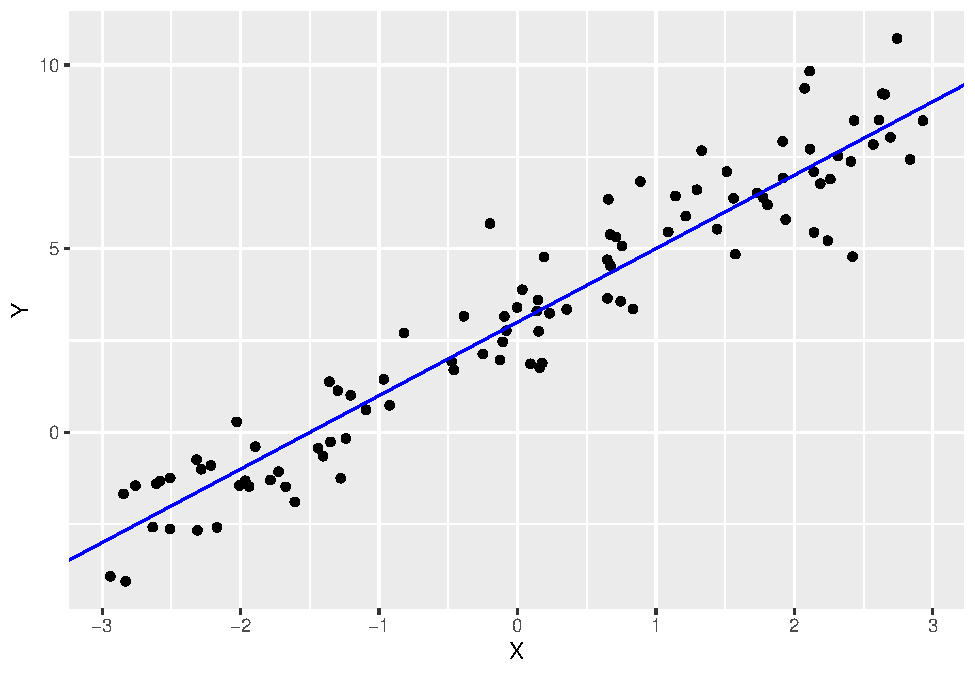
\includegraphics{01-引言_files/figure-latex/basic-glm-1.pdf}
\caption{\label{fig:basic-glm}线性模型Y = 3 + 2X的模拟数据}
\end{figure}

\begin{Shaded}
\begin{Highlighting}[]
\FunctionTok{library}\NormalTok{(}\StringTok{"tidyverse"}\NormalTok{) }\CommentTok{\# if needed}

\FunctionTok{set.seed}\NormalTok{(}\DecValTok{62}\NormalTok{)}

\NormalTok{dat }\OtherTok{\textless{}{-}} \FunctionTok{tibble}\NormalTok{(}\AttributeTok{X =} \FunctionTok{runif}\NormalTok{(}\DecValTok{100}\NormalTok{, }\SpecialCharTok{{-}}\DecValTok{3}\NormalTok{, }\DecValTok{3}\NormalTok{),}
              \AttributeTok{Y =} \DecValTok{3} \SpecialCharTok{+} \DecValTok{2} \SpecialCharTok{*}\NormalTok{ X }\SpecialCharTok{+} \FunctionTok{rnorm}\NormalTok{(}\DecValTok{100}\NormalTok{))}

\FunctionTok{ggplot}\NormalTok{(dat, }\FunctionTok{aes}\NormalTok{(X, Y)) }\SpecialCharTok{+}
  \FunctionTok{geom\_point}\NormalTok{() }\SpecialCharTok{+}
  \FunctionTok{geom\_abline}\NormalTok{(}\AttributeTok{intercept =} \DecValTok{3}\NormalTok{, }\AttributeTok{slope =} \DecValTok{2}\NormalTok{, }\AttributeTok{color =} \StringTok{"blue"}\NormalTok{)}
\end{Highlighting}
\end{Shaded}

你可能会发现上述方程表示的是一条直线(\(y = mx + b\)),其中\(\beta_0\)是截距,\(\beta_1\)是斜率。\(e_i\)是样本\(i\)的模型误差,表示样本观测值\(Y_i\)与给定\(X_i\)的模型预测值之间的差距。

\textbf{表示法惯例}

希腊字母(\(\beta\), \(\rho\), \(\tau\))表示总体参数,通常是未观测到的,需要从数据中估计得到的。当我们想要区分\textbf{估计}参数和真实值时,我们会使用''hat'':如\(\hat{\beta}_0\)表示从数据中估计得到的\(\beta_0\)的值。

大写拉丁字母(\(X\)、\(Y\))表示观测值------即你已经测量过的值,因此是已知的。你也会看到小写拉丁字母(如\(e_i\)),表示统计误差或其他我将称之为派生量或虚拟量的东西(这将在课程后面进行解释)。

\textbf{线性模型中的''线性''并不像你想象的那样!}

许多人认为''线性模型''只能捕捉线性关系,即可以用直线(或平面)来描述的关系。这是错误的。

线性模型是各种项的加权和,每个项都有一个预测变量(或常数)乘上一个系数。在上述模型中,系数是\(\beta_0\)和\(\beta_1\)。你可以用线性模型拟合各种复杂的关系,包括非线性关系,如下所示。

\begin{figure}
\centering
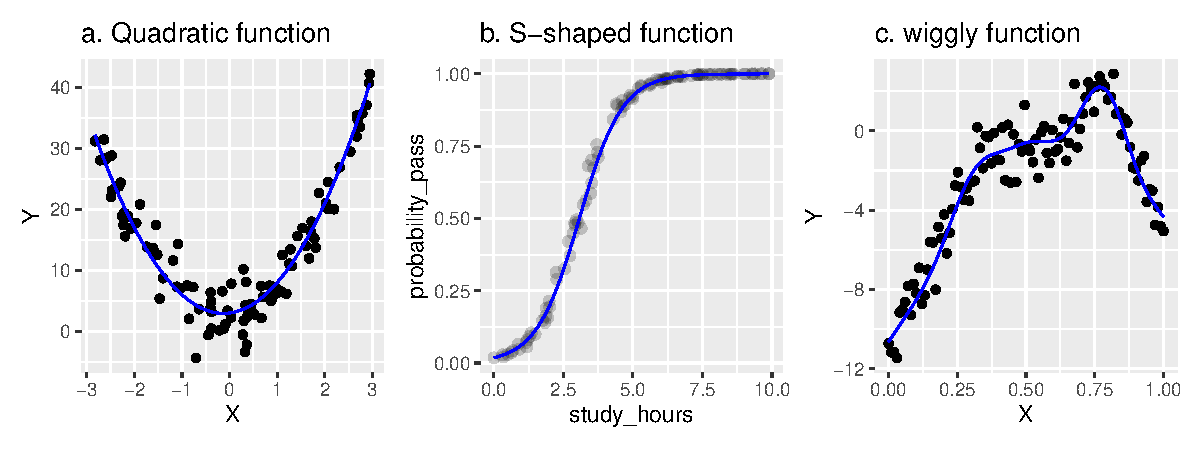
\includegraphics{01-引言_files/figure-latex/tryptych-1.pdf}
\caption{\label{fig:tryptych}用线性模型建模的非线性关系}
\end{figure}

在左边面板中,我们使用线性模型\(Y = \beta_0 + \beta_1 X + \beta_2 X^2\)捕捉了一个二次(抛物线)函数。X和Y之间的关系是非线性的,但模型本身是线性的。我们对预测变量\(X\)进行了平方处理,但系数\(\beta_0\)、\(\beta_1\)和\(\beta_2\)并没有被平方、立方或类似的处理(它们都是''一次幂'')。

在中间面板中,我们使用线性模型捕捉了一个S形函数。在这里,Y变量表示某个事件的概率,例如基于学习时间来预测通过考试的概率。在这种情况下,我们通过在一个特殊的转换空间中估计线性模型来建模X和Y之间的关系,使得X-Y关系是线性的,然后将模型投影回非线性的概率空间(使用''链接函数'')。非线性来自于''链接函数'',但模型本身是线性的。

最后,右边面板展示了一种略显任意的波动模式,由广义可加混合模型捕获------这是一种我们在本课程中不会学到的高级技术。但从根本上说,它仍然是一个线性模型,因为它还是一系列复杂事物(在这种情况下是''基础函数'')的加权和,而系数提供了权重。

线性模型是一个\textbf{系数是线性}的模型;模型中的每个系数(\(\beta_0\)、\(\beta_1\))只允许被设置为一次幂,并且每个项\(\beta_i X_j\)都只涉及单个系数。这些项只能与涉及其他系数的项相加,但不能相乘或相除(如\(Y = \frac{\beta_1}{\beta_2} X\)是不允许的)。

当前课程的一个局限性是主要关注单变量数据,即将单一响应变量作为分析的焦点。通常情况下,你会处理相同对象的多个响应变量,但是同时对它们进行建模在技术上是非常困难的,并且超出了本课程的范围。一种更简单的方法(也是这里采用的方法)是对每个响应变量进行单独的单变量分析。

\hypertarget{ux6df7ux5408ux6a21ux578b}{%
\subsection{混合模型}\label{ux6df7ux5408ux6a21ux578b}}

研究结果的推断或解释的可推广性指的是它能够被轻松应用于超出特定研究背景(对象、刺激、任务等)的情境的程度。最理想的情况是,我们的发现能够适用于人类物种的所有成员,涵盖各种各样的刺激和任务;最糟糕的情况是,它们只能适用于那些受到我们使用的特定刺激的特定的人,在我们研究的特定背景下才观察得到。

研究结果的可推广性取决于几个因素:研究的设计方式、所使用的材料、被试的招募方式、给予被试的任务的性质以及\textbf{数据分析的方式}。在这门课程中我们将重点关注最后一点。在分析一个数据集时,如果你想要提出具有推广性的论断,你必须决定哪些可以算作你研究的重复------关于哪些方面应该在复制中保持不变,以及哪些方面允许变化。

不幸的是,有时你会发现数据以一种不太支持广泛意义上的可推广性的方式进行分析,这往往是因为低估了刺激材料或实验任务的独特特征对观测结果的影响 \citep{yarkoni_2019}。

\hypertarget{ux5173ux4e8eux53efux91cdux590dux6027ux7684ux8bf4ux660e}{%
\section{关于可重复性的说明}\label{ux5173ux4e8eux53efux91cdux590dux6027ux7684ux8bf4ux660e}}

本课程的数据分析是使用R编写脚本进行的。

可重复性指的是在不同情况下重现研究结果的可能性程度。

如果我们能在给定原始数据的情况下得到相同的结果,我们会说这个发现在\emph{分析(analytically)}或\emph{计算(computationally)}上是可重复的。需要注意的是,这与说一个发现\textbf{可复制(replicable)}是不同的。可复制指的是能够在\textbf{新样本}中复制这一发现。对于这些术语并没有广泛的共识,但方便起见,我们可以将分析上的可重复性(reproducibility)和可复制性(replicability)视为两种不同但相关的可重复性(reproducibility)类型,前者反映分析员之间(或同一分析员随时间变化)的可重复性,而后者反映了在被试样本或亚群体之间的可重复性。

确保分析可重复性是一个难题。如果你未能正确记录自己的分析过程,或者你使用的软件被修改或过时并且变得不可用,你可能会在重现自己的发现时遇到麻烦!

分析的另一个重要属性是透明度------在某种研究中所有步骤都可以公开的程度。一项研究可能是透明的但不可重复,反之亦然。使用促进透明度的工作流程非常重要。这使得脚本编程的``编辑--执行''工作流程对于数据分析来说是理想的选择,远远优于大多数商业统计软件的``指向--点击''的工作流程。通过编写代码,你可以使逻辑和决策过程对他人明确,并易于重建。

\hypertarget{ux57faux4e8eux6a21ux62dfux7684ux65b9ux6cd5}{%
\section{基于模拟的方法}\label{ux57faux4e8eux6a21ux62dfux7684ux65b9ux6cd5}}

本课程最后一个重要特点是采用了\textbf{基于模拟的方法}来学习统计模型。通过数据模拟,我们定义一个特定模型来描述感兴趣的总体,然后利用计算机的随机数生成器来模拟从该总体中抽样的过程。我们将在下面看一个简单的例子。

在分析数据时,你会面临的经典问题是你不知道你正在研究的总体的``真实情况''。你从该总体中抽取一个样本,对观测到的数据获取方式做出一些假设,然后利用观察到的数据来估计未知的总体参数及这些参数的不确定性。

数据模拟颠倒了这个过程。你会定义一个模型的参数,代表关于(假设的)总体的真实情况,从中获取数据。然后,你可以像平常一样分析获得的数据,并考察参数估计与真实值之间的对应程度。

让我们看一个例子。假设你对以下问题感兴趣:作为学步幼儿的父母是否会``提高''你的反应能力。如果你曾经照顾过一个幼儿,你就会知道身体危险似乎总是在即------他们可能从刚刚爬上的椅子上摔下来,被门里夹到,头撞在桌子角上等等------所以你需要保持警惕并准备迅速行动。你假设这种警惕会转化为在幼儿不在场的其他情况下的更快反应时间,比如在心理实验室里。因此,你招募了一组有幼儿的父母来实验室。你让每个父母在闪烁的灯光出现时尽快按下按钮,并测量他们的反应时(以毫秒为单位)。对于每个父母,你计算了他们在所有试验中的平均反应时。我们可以使用R中的\texttt{rnorm()}函数模拟50个父母的平均反应时。但在我们开始之前,我们将加载我们需要的包(tidyverse)并设置随机种子(random seed),以确保你(读者)得到和我(作者)相同的随机值。

\begin{Shaded}
\begin{Highlighting}[]
\FunctionTok{library}\NormalTok{(}\StringTok{"tidyverse"}\NormalTok{)}

\FunctionTok{set.seed}\NormalTok{(}\DecValTok{2021}\NormalTok{)  }\CommentTok{\# 可以是任意整数}
\end{Highlighting}
\end{Shaded}

\begin{Shaded}
\begin{Highlighting}[]
\NormalTok{parents }\OtherTok{\textless{}{-}} \FunctionTok{rnorm}\NormalTok{(}\AttributeTok{n =} \DecValTok{50}\NormalTok{, }\AttributeTok{mean =} \DecValTok{480}\NormalTok{, }\AttributeTok{sd =} \DecValTok{40}\NormalTok{)}
\end{Highlighting}
\end{Shaded}

\begin{verbatim}
##  [1] 475.1016 502.0983 493.9460 494.3853 515.9221 403.0972 490.4698 516.6227
##  [9] 480.5509 549.1985 436.7118 469.0870 487.2798 540.3417 544.1788 406.3410
## [17] 544.9324 485.2556 539.2449 540.5327 442.3023 472.5726 435.9550 528.3246
## [25] 415.0025 484.2151 421.7823 465.8394 476.2520 524.0267 401.4470 422.0822
## [33] 520.7777 423.1433 455.8187 416.6610 428.5627 421.8126 476.5172 500.1895
## [41] 484.6555 550.4085 466.1953 564.8000 478.6249 448.3138 539.0206 450.9777
## [49] 492.4952 507.6786
\end{verbatim}

我们选择使用\texttt{rnorm()}来生成数据,这是一个从正态分布中生成随机数的函数,这反映了我们的假设------平均反应时在总体中呈正态分布。正态分布由两个参数定义,一个是均值(通常用希腊字母\(\mu\)表示,发音为''myoo''),另一个是标准差(通常用希腊字母\(\sigma\)表示,发音为''sigma'')。由于我们自己生成了数据,所以\(\mu\)和\(\sigma\)都是已知的,在调用\texttt{rnorm()}时,我们将它们分别设置为480和40。

当然,为了验证我们的假设,我们需要一个对照组,所以我们定义了一个非父母的对照组。我们用相同的方式从这个对照组生成数据,但改变了平均值。

\begin{Shaded}
\begin{Highlighting}[]
\NormalTok{control }\OtherTok{\textless{}{-}} \FunctionTok{rnorm}\NormalTok{(}\AttributeTok{n =} \DecValTok{50}\NormalTok{, }\AttributeTok{mean =} \DecValTok{500}\NormalTok{, }\AttributeTok{sd =} \DecValTok{40}\NormalTok{)}
\end{Highlighting}
\end{Shaded}

让我们将它们放入数据框(tibble)中,以便更容易绘制和分析数据。该数据框中的每一行表示来自特定被试的平均反应时。

\begin{Shaded}
\begin{Highlighting}[]
\NormalTok{dat }\OtherTok{\textless{}{-}} \FunctionTok{tibble}\NormalTok{(}\AttributeTok{group =} \FunctionTok{rep}\NormalTok{(}\FunctionTok{c}\NormalTok{(}\StringTok{"parent"}\NormalTok{, }\StringTok{"control"}\NormalTok{), }\AttributeTok{each =} \DecValTok{50}\NormalTok{),}
              \AttributeTok{rt =} \FunctionTok{c}\NormalTok{(parents, control))}

\NormalTok{dat}
\end{Highlighting}
\end{Shaded}

\begin{verbatim}
## # A tibble: 100 x 2
##    group     rt
##    <chr>  <dbl>
##  1 parent  475.
##  2 parent  502.
##  3 parent  494.
##  4 parent  494.
##  5 parent  516.
##  6 parent  403.
##  7 parent  490.
##  8 parent  517.
##  9 parent  481.
## 10 parent  549.
## # i 90 more rows
\end{verbatim}

下面是对模拟数据的一些尝试。

\begin{enumerate}
\def\labelenumi{\arabic{enumi}.}
\tightlist
\item
  以某种合理的方式绘制数据。
\item
  计算平均值和标准差。它们与总体参数相比如何?
\item
  对这些数据进行t检验。群组效应显著吗?
\end{enumerate}

做完这些后,再做一次,但改变样本量、总体参数或两者都改变。

\hypertarget{ux76f8ux5173ux548cux56deux5f52}{%
\chapter{相关和回归}\label{ux76f8ux5173ux548cux56deux5f52}}

\hypertarget{ux76f8ux5173ux77e9ux9635correlation-matrices}{%
\section{相关矩阵(Correlation matrices)}\label{ux76f8ux5173ux77e9ux9635correlation-matrices}}

你可能已经通过阅读心理学论文对\textbf{相关矩阵}这个概念有所了解。相关矩阵是总结同一个体的多个测量值之间关系的常用方法。

假设你用多个量表测量了心理幸福感。一个问题是这些量表在多大程度上测量了相同的东西。通常,你会查看相关矩阵来探索测量之间所有成对关系。

回忆一下,相关系数量化了两个变量之间关系的\textbf{强度}和\textbf{方向}。它通常用符号\(r\)或\(\rho\)(希腊字母''rho'')表示。相关系数的范围在-1到1之间,其中0表示没有关系,正值反映正相关(一个变量增加,另一个也增加),负值反映负相关(一个变量增加,另一个减少)。

\begin{verbatim}
## Warning in grid.Call(C_textBounds, as.graphicsAnnot(x$label), x$x, x$y, :
## conversion failure on '相关关系: 负相关' in 'mbcsToSbcs': dot substituted for
## <e7>
\end{verbatim}

\begin{verbatim}
## Warning in grid.Call(C_textBounds, as.graphicsAnnot(x$label), x$x, x$y, :
## conversion failure on '相关关系: 负相关' in 'mbcsToSbcs': dot substituted for
## <9b>
\end{verbatim}

\begin{verbatim}
## Warning in grid.Call(C_textBounds, as.graphicsAnnot(x$label), x$x, x$y, :
## conversion failure on '相关关系: 负相关' in 'mbcsToSbcs': dot substituted for
## <b8>
\end{verbatim}

\begin{verbatim}
## Warning in grid.Call(C_textBounds, as.graphicsAnnot(x$label), x$x, x$y, :
## conversion failure on '相关关系: 负相关' in 'mbcsToSbcs': dot substituted for
## <e5>
\end{verbatim}

\begin{verbatim}
## Warning in grid.Call(C_textBounds, as.graphicsAnnot(x$label), x$x, x$y, :
## conversion failure on '相关关系: 负相关' in 'mbcsToSbcs': dot substituted for
## <85>
\end{verbatim}

\begin{verbatim}
## Warning in grid.Call(C_textBounds, as.graphicsAnnot(x$label), x$x, x$y, :
## conversion failure on '相关关系: 负相关' in 'mbcsToSbcs': dot substituted for
## <b3>
\end{verbatim}

\begin{verbatim}
## Warning in grid.Call(C_textBounds, as.graphicsAnnot(x$label), x$x, x$y, :
## conversion failure on '相关关系: 负相关' in 'mbcsToSbcs': dot substituted for
## <e5>
\end{verbatim}

\begin{verbatim}
## Warning in grid.Call(C_textBounds, as.graphicsAnnot(x$label), x$x, x$y, :
## conversion failure on '相关关系: 负相关' in 'mbcsToSbcs': dot substituted for
## <85>
\end{verbatim}

\begin{verbatim}
## Warning in grid.Call(C_textBounds, as.graphicsAnnot(x$label), x$x, x$y, :
## conversion failure on '相关关系: 负相关' in 'mbcsToSbcs': dot substituted for
## <b3>
\end{verbatim}

\begin{verbatim}
## Warning in grid.Call(C_textBounds, as.graphicsAnnot(x$label), x$x, x$y, :
## conversion failure on '相关关系: 负相关' in 'mbcsToSbcs': dot substituted for
## <e7>
\end{verbatim}

\begin{verbatim}
## Warning in grid.Call(C_textBounds, as.graphicsAnnot(x$label), x$x, x$y, :
## conversion failure on '相关关系: 负相关' in 'mbcsToSbcs': dot substituted for
## <b3>
\end{verbatim}

\begin{verbatim}
## Warning in grid.Call(C_textBounds, as.graphicsAnnot(x$label), x$x, x$y, :
## conversion failure on '相关关系: 负相关' in 'mbcsToSbcs': dot substituted for
## <bb>
\end{verbatim}

\begin{verbatim}
## Warning in grid.Call(C_textBounds, as.graphicsAnnot(x$label), x$x, x$y, :
## conversion failure on '相关关系: 负相关' in 'mbcsToSbcs': dot substituted for
## <e8>
\end{verbatim}

\begin{verbatim}
## Warning in grid.Call(C_textBounds, as.graphicsAnnot(x$label), x$x, x$y, :
## conversion failure on '相关关系: 负相关' in 'mbcsToSbcs': dot substituted for
## <b4>
\end{verbatim}

\begin{verbatim}
## Warning in grid.Call(C_textBounds, as.graphicsAnnot(x$label), x$x, x$y, :
## conversion failure on '相关关系: 负相关' in 'mbcsToSbcs': dot substituted for
## <9f>
\end{verbatim}

\begin{verbatim}
## Warning in grid.Call(C_textBounds, as.graphicsAnnot(x$label), x$x, x$y, :
## conversion failure on '相关关系: 负相关' in 'mbcsToSbcs': dot substituted for
## <e7>
\end{verbatim}

\begin{verbatim}
## Warning in grid.Call(C_textBounds, as.graphicsAnnot(x$label), x$x, x$y, :
## conversion failure on '相关关系: 负相关' in 'mbcsToSbcs': dot substituted for
## <9b>
\end{verbatim}

\begin{verbatim}
## Warning in grid.Call(C_textBounds, as.graphicsAnnot(x$label), x$x, x$y, :
## conversion failure on '相关关系: 负相关' in 'mbcsToSbcs': dot substituted for
## <b8>
\end{verbatim}

\begin{verbatim}
## Warning in grid.Call(C_textBounds, as.graphicsAnnot(x$label), x$x, x$y, :
## conversion failure on '相关关系: 负相关' in 'mbcsToSbcs': dot substituted for
## <e5>
\end{verbatim}

\begin{verbatim}
## Warning in grid.Call(C_textBounds, as.graphicsAnnot(x$label), x$x, x$y, :
## conversion failure on '相关关系: 负相关' in 'mbcsToSbcs': dot substituted for
## <85>
\end{verbatim}

\begin{verbatim}
## Warning in grid.Call(C_textBounds, as.graphicsAnnot(x$label), x$x, x$y, :
## conversion failure on '相关关系: 负相关' in 'mbcsToSbcs': dot substituted for
## <b3>
\end{verbatim}

\begin{verbatim}
## Warning in grid.Call(C_textBounds, as.graphicsAnnot(x$label), x$x, x$y, :
## conversion failure on '相关关系: 无相关' in 'mbcsToSbcs': dot substituted for
## <e7>
\end{verbatim}

\begin{verbatim}
## Warning in grid.Call(C_textBounds, as.graphicsAnnot(x$label), x$x, x$y, :
## conversion failure on '相关关系: 无相关' in 'mbcsToSbcs': dot substituted for
## <9b>
\end{verbatim}

\begin{verbatim}
## Warning in grid.Call(C_textBounds, as.graphicsAnnot(x$label), x$x, x$y, :
## conversion failure on '相关关系: 无相关' in 'mbcsToSbcs': dot substituted for
## <b8>
\end{verbatim}

\begin{verbatim}
## Warning in grid.Call(C_textBounds, as.graphicsAnnot(x$label), x$x, x$y, :
## conversion failure on '相关关系: 无相关' in 'mbcsToSbcs': dot substituted for
## <e5>
\end{verbatim}

\begin{verbatim}
## Warning in grid.Call(C_textBounds, as.graphicsAnnot(x$label), x$x, x$y, :
## conversion failure on '相关关系: 无相关' in 'mbcsToSbcs': dot substituted for
## <85>
\end{verbatim}

\begin{verbatim}
## Warning in grid.Call(C_textBounds, as.graphicsAnnot(x$label), x$x, x$y, :
## conversion failure on '相关关系: 无相关' in 'mbcsToSbcs': dot substituted for
## <b3>
\end{verbatim}

\begin{verbatim}
## Warning in grid.Call(C_textBounds, as.graphicsAnnot(x$label), x$x, x$y, :
## conversion failure on '相关关系: 无相关' in 'mbcsToSbcs': dot substituted for
## <e5>
\end{verbatim}

\begin{verbatim}
## Warning in grid.Call(C_textBounds, as.graphicsAnnot(x$label), x$x, x$y, :
## conversion failure on '相关关系: 无相关' in 'mbcsToSbcs': dot substituted for
## <85>
\end{verbatim}

\begin{verbatim}
## Warning in grid.Call(C_textBounds, as.graphicsAnnot(x$label), x$x, x$y, :
## conversion failure on '相关关系: 无相关' in 'mbcsToSbcs': dot substituted for
## <b3>
\end{verbatim}

\begin{verbatim}
## Warning in grid.Call(C_textBounds, as.graphicsAnnot(x$label), x$x, x$y, :
## conversion failure on '相关关系: 无相关' in 'mbcsToSbcs': dot substituted for
## <e7>
\end{verbatim}

\begin{verbatim}
## Warning in grid.Call(C_textBounds, as.graphicsAnnot(x$label), x$x, x$y, :
## conversion failure on '相关关系: 无相关' in 'mbcsToSbcs': dot substituted for
## <b3>
\end{verbatim}

\begin{verbatim}
## Warning in grid.Call(C_textBounds, as.graphicsAnnot(x$label), x$x, x$y, :
## conversion failure on '相关关系: 无相关' in 'mbcsToSbcs': dot substituted for
## <bb>
\end{verbatim}

\begin{verbatim}
## Warning in grid.Call(C_textBounds, as.graphicsAnnot(x$label), x$x, x$y, :
## conversion failure on '相关关系: 无相关' in 'mbcsToSbcs': dot substituted for
## <e6>
\end{verbatim}

\begin{verbatim}
## Warning in grid.Call(C_textBounds, as.graphicsAnnot(x$label), x$x, x$y, :
## conversion failure on '相关关系: 无相关' in 'mbcsToSbcs': dot substituted for
## <97>
\end{verbatim}

\begin{verbatim}
## Warning in grid.Call(C_textBounds, as.graphicsAnnot(x$label), x$x, x$y, :
## conversion failure on '相关关系: 无相关' in 'mbcsToSbcs': dot substituted for
## <a0>
\end{verbatim}

\begin{verbatim}
## Warning in grid.Call(C_textBounds, as.graphicsAnnot(x$label), x$x, x$y, :
## conversion failure on '相关关系: 无相关' in 'mbcsToSbcs': dot substituted for
## <e7>
\end{verbatim}

\begin{verbatim}
## Warning in grid.Call(C_textBounds, as.graphicsAnnot(x$label), x$x, x$y, :
## conversion failure on '相关关系: 无相关' in 'mbcsToSbcs': dot substituted for
## <9b>
\end{verbatim}

\begin{verbatim}
## Warning in grid.Call(C_textBounds, as.graphicsAnnot(x$label), x$x, x$y, :
## conversion failure on '相关关系: 无相关' in 'mbcsToSbcs': dot substituted for
## <b8>
\end{verbatim}

\begin{verbatim}
## Warning in grid.Call(C_textBounds, as.graphicsAnnot(x$label), x$x, x$y, :
## conversion failure on '相关关系: 无相关' in 'mbcsToSbcs': dot substituted for
## <e5>
\end{verbatim}

\begin{verbatim}
## Warning in grid.Call(C_textBounds, as.graphicsAnnot(x$label), x$x, x$y, :
## conversion failure on '相关关系: 无相关' in 'mbcsToSbcs': dot substituted for
## <85>
\end{verbatim}

\begin{verbatim}
## Warning in grid.Call(C_textBounds, as.graphicsAnnot(x$label), x$x, x$y, :
## conversion failure on '相关关系: 无相关' in 'mbcsToSbcs': dot substituted for
## <b3>
\end{verbatim}

\begin{verbatim}
## Warning in grid.Call(C_textBounds, as.graphicsAnnot(x$label), x$x, x$y, :
## conversion failure on '相关关系: 正相关' in 'mbcsToSbcs': dot substituted for
## <e7>
\end{verbatim}

\begin{verbatim}
## Warning in grid.Call(C_textBounds, as.graphicsAnnot(x$label), x$x, x$y, :
## conversion failure on '相关关系: 正相关' in 'mbcsToSbcs': dot substituted for
## <9b>
\end{verbatim}

\begin{verbatim}
## Warning in grid.Call(C_textBounds, as.graphicsAnnot(x$label), x$x, x$y, :
## conversion failure on '相关关系: 正相关' in 'mbcsToSbcs': dot substituted for
## <b8>
\end{verbatim}

\begin{verbatim}
## Warning in grid.Call(C_textBounds, as.graphicsAnnot(x$label), x$x, x$y, :
## conversion failure on '相关关系: 正相关' in 'mbcsToSbcs': dot substituted for
## <e5>
\end{verbatim}

\begin{verbatim}
## Warning in grid.Call(C_textBounds, as.graphicsAnnot(x$label), x$x, x$y, :
## conversion failure on '相关关系: 正相关' in 'mbcsToSbcs': dot substituted for
## <85>
\end{verbatim}

\begin{verbatim}
## Warning in grid.Call(C_textBounds, as.graphicsAnnot(x$label), x$x, x$y, :
## conversion failure on '相关关系: 正相关' in 'mbcsToSbcs': dot substituted for
## <b3>
\end{verbatim}

\begin{verbatim}
## Warning in grid.Call(C_textBounds, as.graphicsAnnot(x$label), x$x, x$y, :
## conversion failure on '相关关系: 正相关' in 'mbcsToSbcs': dot substituted for
## <e5>
\end{verbatim}

\begin{verbatim}
## Warning in grid.Call(C_textBounds, as.graphicsAnnot(x$label), x$x, x$y, :
## conversion failure on '相关关系: 正相关' in 'mbcsToSbcs': dot substituted for
## <85>
\end{verbatim}

\begin{verbatim}
## Warning in grid.Call(C_textBounds, as.graphicsAnnot(x$label), x$x, x$y, :
## conversion failure on '相关关系: 正相关' in 'mbcsToSbcs': dot substituted for
## <b3>
\end{verbatim}

\begin{verbatim}
## Warning in grid.Call(C_textBounds, as.graphicsAnnot(x$label), x$x, x$y, :
## conversion failure on '相关关系: 正相关' in 'mbcsToSbcs': dot substituted for
## <e7>
\end{verbatim}

\begin{verbatim}
## Warning in grid.Call(C_textBounds, as.graphicsAnnot(x$label), x$x, x$y, :
## conversion failure on '相关关系: 正相关' in 'mbcsToSbcs': dot substituted for
## <b3>
\end{verbatim}

\begin{verbatim}
## Warning in grid.Call(C_textBounds, as.graphicsAnnot(x$label), x$x, x$y, :
## conversion failure on '相关关系: 正相关' in 'mbcsToSbcs': dot substituted for
## <bb>
\end{verbatim}

\begin{verbatim}
## Warning in grid.Call(C_textBounds, as.graphicsAnnot(x$label), x$x, x$y, :
## conversion failure on '相关关系: 正相关' in 'mbcsToSbcs': dot substituted for
## <e6>
\end{verbatim}

\begin{verbatim}
## Warning in grid.Call(C_textBounds, as.graphicsAnnot(x$label), x$x, x$y, :
## conversion failure on '相关关系: 正相关' in 'mbcsToSbcs': dot substituted for
## <ad>
\end{verbatim}

\begin{verbatim}
## Warning in grid.Call(C_textBounds, as.graphicsAnnot(x$label), x$x, x$y, :
## conversion failure on '相关关系: 正相关' in 'mbcsToSbcs': dot substituted for
## <a3>
\end{verbatim}

\begin{verbatim}
## Warning in grid.Call(C_textBounds, as.graphicsAnnot(x$label), x$x, x$y, :
## conversion failure on '相关关系: 正相关' in 'mbcsToSbcs': dot substituted for
## <e7>
\end{verbatim}

\begin{verbatim}
## Warning in grid.Call(C_textBounds, as.graphicsAnnot(x$label), x$x, x$y, :
## conversion failure on '相关关系: 正相关' in 'mbcsToSbcs': dot substituted for
## <9b>
\end{verbatim}

\begin{verbatim}
## Warning in grid.Call(C_textBounds, as.graphicsAnnot(x$label), x$x, x$y, :
## conversion failure on '相关关系: 正相关' in 'mbcsToSbcs': dot substituted for
## <b8>
\end{verbatim}

\begin{verbatim}
## Warning in grid.Call(C_textBounds, as.graphicsAnnot(x$label), x$x, x$y, :
## conversion failure on '相关关系: 正相关' in 'mbcsToSbcs': dot substituted for
## <e5>
\end{verbatim}

\begin{verbatim}
## Warning in grid.Call(C_textBounds, as.graphicsAnnot(x$label), x$x, x$y, :
## conversion failure on '相关关系: 正相关' in 'mbcsToSbcs': dot substituted for
## <85>
\end{verbatim}

\begin{verbatim}
## Warning in grid.Call(C_textBounds, as.graphicsAnnot(x$label), x$x, x$y, :
## conversion failure on '相关关系: 正相关' in 'mbcsToSbcs': dot substituted for
## <b3>
\end{verbatim}

\begin{verbatim}
## Warning in grid.Call(C_textBounds, as.graphicsAnnot(x$label), x$x, x$y, :
## conversion failure on '相关关系: 负相关' in 'mbcsToSbcs': dot substituted for
## <e7>
\end{verbatim}

\begin{verbatim}
## Warning in grid.Call(C_textBounds, as.graphicsAnnot(x$label), x$x, x$y, :
## conversion failure on '相关关系: 负相关' in 'mbcsToSbcs': dot substituted for
## <9b>
\end{verbatim}

\begin{verbatim}
## Warning in grid.Call(C_textBounds, as.graphicsAnnot(x$label), x$x, x$y, :
## conversion failure on '相关关系: 负相关' in 'mbcsToSbcs': dot substituted for
## <b8>
\end{verbatim}

\begin{verbatim}
## Warning in grid.Call(C_textBounds, as.graphicsAnnot(x$label), x$x, x$y, :
## conversion failure on '相关关系: 负相关' in 'mbcsToSbcs': dot substituted for
## <e5>
\end{verbatim}

\begin{verbatim}
## Warning in grid.Call(C_textBounds, as.graphicsAnnot(x$label), x$x, x$y, :
## conversion failure on '相关关系: 负相关' in 'mbcsToSbcs': dot substituted for
## <85>
\end{verbatim}

\begin{verbatim}
## Warning in grid.Call(C_textBounds, as.graphicsAnnot(x$label), x$x, x$y, :
## conversion failure on '相关关系: 负相关' in 'mbcsToSbcs': dot substituted for
## <b3>
\end{verbatim}

\begin{verbatim}
## Warning in grid.Call(C_textBounds, as.graphicsAnnot(x$label), x$x, x$y, :
## conversion failure on '相关关系: 负相关' in 'mbcsToSbcs': dot substituted for
## <e5>
\end{verbatim}

\begin{verbatim}
## Warning in grid.Call(C_textBounds, as.graphicsAnnot(x$label), x$x, x$y, :
## conversion failure on '相关关系: 负相关' in 'mbcsToSbcs': dot substituted for
## <85>
\end{verbatim}

\begin{verbatim}
## Warning in grid.Call(C_textBounds, as.graphicsAnnot(x$label), x$x, x$y, :
## conversion failure on '相关关系: 负相关' in 'mbcsToSbcs': dot substituted for
## <b3>
\end{verbatim}

\begin{verbatim}
## Warning in grid.Call(C_textBounds, as.graphicsAnnot(x$label), x$x, x$y, :
## conversion failure on '相关关系: 负相关' in 'mbcsToSbcs': dot substituted for
## <e7>
\end{verbatim}

\begin{verbatim}
## Warning in grid.Call(C_textBounds, as.graphicsAnnot(x$label), x$x, x$y, :
## conversion failure on '相关关系: 负相关' in 'mbcsToSbcs': dot substituted for
## <b3>
\end{verbatim}

\begin{verbatim}
## Warning in grid.Call(C_textBounds, as.graphicsAnnot(x$label), x$x, x$y, :
## conversion failure on '相关关系: 负相关' in 'mbcsToSbcs': dot substituted for
## <bb>
\end{verbatim}

\begin{verbatim}
## Warning in grid.Call(C_textBounds, as.graphicsAnnot(x$label), x$x, x$y, :
## conversion failure on '相关关系: 负相关' in 'mbcsToSbcs': dot substituted for
## <e8>
\end{verbatim}

\begin{verbatim}
## Warning in grid.Call(C_textBounds, as.graphicsAnnot(x$label), x$x, x$y, :
## conversion failure on '相关关系: 负相关' in 'mbcsToSbcs': dot substituted for
## <b4>
\end{verbatim}

\begin{verbatim}
## Warning in grid.Call(C_textBounds, as.graphicsAnnot(x$label), x$x, x$y, :
## conversion failure on '相关关系: 负相关' in 'mbcsToSbcs': dot substituted for
## <9f>
\end{verbatim}

\begin{verbatim}
## Warning in grid.Call(C_textBounds, as.graphicsAnnot(x$label), x$x, x$y, :
## conversion failure on '相关关系: 负相关' in 'mbcsToSbcs': dot substituted for
## <e7>
\end{verbatim}

\begin{verbatim}
## Warning in grid.Call(C_textBounds, as.graphicsAnnot(x$label), x$x, x$y, :
## conversion failure on '相关关系: 负相关' in 'mbcsToSbcs': dot substituted for
## <9b>
\end{verbatim}

\begin{verbatim}
## Warning in grid.Call(C_textBounds, as.graphicsAnnot(x$label), x$x, x$y, :
## conversion failure on '相关关系: 负相关' in 'mbcsToSbcs': dot substituted for
## <b8>
\end{verbatim}

\begin{verbatim}
## Warning in grid.Call(C_textBounds, as.graphicsAnnot(x$label), x$x, x$y, :
## conversion failure on '相关关系: 负相关' in 'mbcsToSbcs': dot substituted for
## <e5>
\end{verbatim}

\begin{verbatim}
## Warning in grid.Call(C_textBounds, as.graphicsAnnot(x$label), x$x, x$y, :
## conversion failure on '相关关系: 负相关' in 'mbcsToSbcs': dot substituted for
## <85>
\end{verbatim}

\begin{verbatim}
## Warning in grid.Call(C_textBounds, as.graphicsAnnot(x$label), x$x, x$y, :
## conversion failure on '相关关系: 负相关' in 'mbcsToSbcs': dot substituted for
## <b3>
\end{verbatim}

\begin{verbatim}
## Warning in grid.Call(C_textBounds, as.graphicsAnnot(x$label), x$x, x$y, :
## conversion failure on '相关关系: 无相关' in 'mbcsToSbcs': dot substituted for
## <e7>
\end{verbatim}

\begin{verbatim}
## Warning in grid.Call(C_textBounds, as.graphicsAnnot(x$label), x$x, x$y, :
## conversion failure on '相关关系: 无相关' in 'mbcsToSbcs': dot substituted for
## <9b>
\end{verbatim}

\begin{verbatim}
## Warning in grid.Call(C_textBounds, as.graphicsAnnot(x$label), x$x, x$y, :
## conversion failure on '相关关系: 无相关' in 'mbcsToSbcs': dot substituted for
## <b8>
\end{verbatim}

\begin{verbatim}
## Warning in grid.Call(C_textBounds, as.graphicsAnnot(x$label), x$x, x$y, :
## conversion failure on '相关关系: 无相关' in 'mbcsToSbcs': dot substituted for
## <e5>
\end{verbatim}

\begin{verbatim}
## Warning in grid.Call(C_textBounds, as.graphicsAnnot(x$label), x$x, x$y, :
## conversion failure on '相关关系: 无相关' in 'mbcsToSbcs': dot substituted for
## <85>
\end{verbatim}

\begin{verbatim}
## Warning in grid.Call(C_textBounds, as.graphicsAnnot(x$label), x$x, x$y, :
## conversion failure on '相关关系: 无相关' in 'mbcsToSbcs': dot substituted for
## <b3>
\end{verbatim}

\begin{verbatim}
## Warning in grid.Call(C_textBounds, as.graphicsAnnot(x$label), x$x, x$y, :
## conversion failure on '相关关系: 无相关' in 'mbcsToSbcs': dot substituted for
## <e5>
\end{verbatim}

\begin{verbatim}
## Warning in grid.Call(C_textBounds, as.graphicsAnnot(x$label), x$x, x$y, :
## conversion failure on '相关关系: 无相关' in 'mbcsToSbcs': dot substituted for
## <85>
\end{verbatim}

\begin{verbatim}
## Warning in grid.Call(C_textBounds, as.graphicsAnnot(x$label), x$x, x$y, :
## conversion failure on '相关关系: 无相关' in 'mbcsToSbcs': dot substituted for
## <b3>
\end{verbatim}

\begin{verbatim}
## Warning in grid.Call(C_textBounds, as.graphicsAnnot(x$label), x$x, x$y, :
## conversion failure on '相关关系: 无相关' in 'mbcsToSbcs': dot substituted for
## <e7>
\end{verbatim}

\begin{verbatim}
## Warning in grid.Call(C_textBounds, as.graphicsAnnot(x$label), x$x, x$y, :
## conversion failure on '相关关系: 无相关' in 'mbcsToSbcs': dot substituted for
## <b3>
\end{verbatim}

\begin{verbatim}
## Warning in grid.Call(C_textBounds, as.graphicsAnnot(x$label), x$x, x$y, :
## conversion failure on '相关关系: 无相关' in 'mbcsToSbcs': dot substituted for
## <bb>
\end{verbatim}

\begin{verbatim}
## Warning in grid.Call(C_textBounds, as.graphicsAnnot(x$label), x$x, x$y, :
## conversion failure on '相关关系: 无相关' in 'mbcsToSbcs': dot substituted for
## <e6>
\end{verbatim}

\begin{verbatim}
## Warning in grid.Call(C_textBounds, as.graphicsAnnot(x$label), x$x, x$y, :
## conversion failure on '相关关系: 无相关' in 'mbcsToSbcs': dot substituted for
## <97>
\end{verbatim}

\begin{verbatim}
## Warning in grid.Call(C_textBounds, as.graphicsAnnot(x$label), x$x, x$y, :
## conversion failure on '相关关系: 无相关' in 'mbcsToSbcs': dot substituted for
## <a0>
\end{verbatim}

\begin{verbatim}
## Warning in grid.Call(C_textBounds, as.graphicsAnnot(x$label), x$x, x$y, :
## conversion failure on '相关关系: 无相关' in 'mbcsToSbcs': dot substituted for
## <e7>
\end{verbatim}

\begin{verbatim}
## Warning in grid.Call(C_textBounds, as.graphicsAnnot(x$label), x$x, x$y, :
## conversion failure on '相关关系: 无相关' in 'mbcsToSbcs': dot substituted for
## <9b>
\end{verbatim}

\begin{verbatim}
## Warning in grid.Call(C_textBounds, as.graphicsAnnot(x$label), x$x, x$y, :
## conversion failure on '相关关系: 无相关' in 'mbcsToSbcs': dot substituted for
## <b8>
\end{verbatim}

\begin{verbatim}
## Warning in grid.Call(C_textBounds, as.graphicsAnnot(x$label), x$x, x$y, :
## conversion failure on '相关关系: 无相关' in 'mbcsToSbcs': dot substituted for
## <e5>
\end{verbatim}

\begin{verbatim}
## Warning in grid.Call(C_textBounds, as.graphicsAnnot(x$label), x$x, x$y, :
## conversion failure on '相关关系: 无相关' in 'mbcsToSbcs': dot substituted for
## <85>
\end{verbatim}

\begin{verbatim}
## Warning in grid.Call(C_textBounds, as.graphicsAnnot(x$label), x$x, x$y, :
## conversion failure on '相关关系: 无相关' in 'mbcsToSbcs': dot substituted for
## <b3>
\end{verbatim}

\begin{verbatim}
## Warning in grid.Call(C_textBounds, as.graphicsAnnot(x$label), x$x, x$y, :
## conversion failure on '相关关系: 正相关' in 'mbcsToSbcs': dot substituted for
## <e7>
\end{verbatim}

\begin{verbatim}
## Warning in grid.Call(C_textBounds, as.graphicsAnnot(x$label), x$x, x$y, :
## conversion failure on '相关关系: 正相关' in 'mbcsToSbcs': dot substituted for
## <9b>
\end{verbatim}

\begin{verbatim}
## Warning in grid.Call(C_textBounds, as.graphicsAnnot(x$label), x$x, x$y, :
## conversion failure on '相关关系: 正相关' in 'mbcsToSbcs': dot substituted for
## <b8>
\end{verbatim}

\begin{verbatim}
## Warning in grid.Call(C_textBounds, as.graphicsAnnot(x$label), x$x, x$y, :
## conversion failure on '相关关系: 正相关' in 'mbcsToSbcs': dot substituted for
## <e5>
\end{verbatim}

\begin{verbatim}
## Warning in grid.Call(C_textBounds, as.graphicsAnnot(x$label), x$x, x$y, :
## conversion failure on '相关关系: 正相关' in 'mbcsToSbcs': dot substituted for
## <85>
\end{verbatim}

\begin{verbatim}
## Warning in grid.Call(C_textBounds, as.graphicsAnnot(x$label), x$x, x$y, :
## conversion failure on '相关关系: 正相关' in 'mbcsToSbcs': dot substituted for
## <b3>
\end{verbatim}

\begin{verbatim}
## Warning in grid.Call(C_textBounds, as.graphicsAnnot(x$label), x$x, x$y, :
## conversion failure on '相关关系: 正相关' in 'mbcsToSbcs': dot substituted for
## <e5>
\end{verbatim}

\begin{verbatim}
## Warning in grid.Call(C_textBounds, as.graphicsAnnot(x$label), x$x, x$y, :
## conversion failure on '相关关系: 正相关' in 'mbcsToSbcs': dot substituted for
## <85>
\end{verbatim}

\begin{verbatim}
## Warning in grid.Call(C_textBounds, as.graphicsAnnot(x$label), x$x, x$y, :
## conversion failure on '相关关系: 正相关' in 'mbcsToSbcs': dot substituted for
## <b3>
\end{verbatim}

\begin{verbatim}
## Warning in grid.Call(C_textBounds, as.graphicsAnnot(x$label), x$x, x$y, :
## conversion failure on '相关关系: 正相关' in 'mbcsToSbcs': dot substituted for
## <e7>
\end{verbatim}

\begin{verbatim}
## Warning in grid.Call(C_textBounds, as.graphicsAnnot(x$label), x$x, x$y, :
## conversion failure on '相关关系: 正相关' in 'mbcsToSbcs': dot substituted for
## <b3>
\end{verbatim}

\begin{verbatim}
## Warning in grid.Call(C_textBounds, as.graphicsAnnot(x$label), x$x, x$y, :
## conversion failure on '相关关系: 正相关' in 'mbcsToSbcs': dot substituted for
## <bb>
\end{verbatim}

\begin{verbatim}
## Warning in grid.Call(C_textBounds, as.graphicsAnnot(x$label), x$x, x$y, :
## conversion failure on '相关关系: 正相关' in 'mbcsToSbcs': dot substituted for
## <e6>
\end{verbatim}

\begin{verbatim}
## Warning in grid.Call(C_textBounds, as.graphicsAnnot(x$label), x$x, x$y, :
## conversion failure on '相关关系: 正相关' in 'mbcsToSbcs': dot substituted for
## <ad>
\end{verbatim}

\begin{verbatim}
## Warning in grid.Call(C_textBounds, as.graphicsAnnot(x$label), x$x, x$y, :
## conversion failure on '相关关系: 正相关' in 'mbcsToSbcs': dot substituted for
## <a3>
\end{verbatim}

\begin{verbatim}
## Warning in grid.Call(C_textBounds, as.graphicsAnnot(x$label), x$x, x$y, :
## conversion failure on '相关关系: 正相关' in 'mbcsToSbcs': dot substituted for
## <e7>
\end{verbatim}

\begin{verbatim}
## Warning in grid.Call(C_textBounds, as.graphicsAnnot(x$label), x$x, x$y, :
## conversion failure on '相关关系: 正相关' in 'mbcsToSbcs': dot substituted for
## <9b>
\end{verbatim}

\begin{verbatim}
## Warning in grid.Call(C_textBounds, as.graphicsAnnot(x$label), x$x, x$y, :
## conversion failure on '相关关系: 正相关' in 'mbcsToSbcs': dot substituted for
## <b8>
\end{verbatim}

\begin{verbatim}
## Warning in grid.Call(C_textBounds, as.graphicsAnnot(x$label), x$x, x$y, :
## conversion failure on '相关关系: 正相关' in 'mbcsToSbcs': dot substituted for
## <e5>
\end{verbatim}

\begin{verbatim}
## Warning in grid.Call(C_textBounds, as.graphicsAnnot(x$label), x$x, x$y, :
## conversion failure on '相关关系: 正相关' in 'mbcsToSbcs': dot substituted for
## <85>
\end{verbatim}

\begin{verbatim}
## Warning in grid.Call(C_textBounds, as.graphicsAnnot(x$label), x$x, x$y, :
## conversion failure on '相关关系: 正相关' in 'mbcsToSbcs': dot substituted for
## <b3>
\end{verbatim}

\begin{verbatim}
## Warning in grid.Call(C_textBounds, as.graphicsAnnot(x$label), x$x, x$y, :
## conversion failure on '相关关系: 负相关' in 'mbcsToSbcs': dot substituted for
## <e7>
\end{verbatim}

\begin{verbatim}
## Warning in grid.Call(C_textBounds, as.graphicsAnnot(x$label), x$x, x$y, :
## conversion failure on '相关关系: 负相关' in 'mbcsToSbcs': dot substituted for
## <9b>
\end{verbatim}

\begin{verbatim}
## Warning in grid.Call(C_textBounds, as.graphicsAnnot(x$label), x$x, x$y, :
## conversion failure on '相关关系: 负相关' in 'mbcsToSbcs': dot substituted for
## <b8>
\end{verbatim}

\begin{verbatim}
## Warning in grid.Call(C_textBounds, as.graphicsAnnot(x$label), x$x, x$y, :
## conversion failure on '相关关系: 负相关' in 'mbcsToSbcs': dot substituted for
## <e5>
\end{verbatim}

\begin{verbatim}
## Warning in grid.Call(C_textBounds, as.graphicsAnnot(x$label), x$x, x$y, :
## conversion failure on '相关关系: 负相关' in 'mbcsToSbcs': dot substituted for
## <85>
\end{verbatim}

\begin{verbatim}
## Warning in grid.Call(C_textBounds, as.graphicsAnnot(x$label), x$x, x$y, :
## conversion failure on '相关关系: 负相关' in 'mbcsToSbcs': dot substituted for
## <b3>
\end{verbatim}

\begin{verbatim}
## Warning in grid.Call(C_textBounds, as.graphicsAnnot(x$label), x$x, x$y, :
## conversion failure on '相关关系: 负相关' in 'mbcsToSbcs': dot substituted for
## <e5>
\end{verbatim}

\begin{verbatim}
## Warning in grid.Call(C_textBounds, as.graphicsAnnot(x$label), x$x, x$y, :
## conversion failure on '相关关系: 负相关' in 'mbcsToSbcs': dot substituted for
## <85>
\end{verbatim}

\begin{verbatim}
## Warning in grid.Call(C_textBounds, as.graphicsAnnot(x$label), x$x, x$y, :
## conversion failure on '相关关系: 负相关' in 'mbcsToSbcs': dot substituted for
## <b3>
\end{verbatim}

\begin{verbatim}
## Warning in grid.Call(C_textBounds, as.graphicsAnnot(x$label), x$x, x$y, :
## conversion failure on '相关关系: 负相关' in 'mbcsToSbcs': dot substituted for
## <e7>
\end{verbatim}

\begin{verbatim}
## Warning in grid.Call(C_textBounds, as.graphicsAnnot(x$label), x$x, x$y, :
## conversion failure on '相关关系: 负相关' in 'mbcsToSbcs': dot substituted for
## <b3>
\end{verbatim}

\begin{verbatim}
## Warning in grid.Call(C_textBounds, as.graphicsAnnot(x$label), x$x, x$y, :
## conversion failure on '相关关系: 负相关' in 'mbcsToSbcs': dot substituted for
## <bb>
\end{verbatim}

\begin{verbatim}
## Warning in grid.Call(C_textBounds, as.graphicsAnnot(x$label), x$x, x$y, :
## conversion failure on '相关关系: 负相关' in 'mbcsToSbcs': dot substituted for
## <e8>
\end{verbatim}

\begin{verbatim}
## Warning in grid.Call(C_textBounds, as.graphicsAnnot(x$label), x$x, x$y, :
## conversion failure on '相关关系: 负相关' in 'mbcsToSbcs': dot substituted for
## <b4>
\end{verbatim}

\begin{verbatim}
## Warning in grid.Call(C_textBounds, as.graphicsAnnot(x$label), x$x, x$y, :
## conversion failure on '相关关系: 负相关' in 'mbcsToSbcs': dot substituted for
## <9f>
\end{verbatim}

\begin{verbatim}
## Warning in grid.Call(C_textBounds, as.graphicsAnnot(x$label), x$x, x$y, :
## conversion failure on '相关关系: 负相关' in 'mbcsToSbcs': dot substituted for
## <e7>
\end{verbatim}

\begin{verbatim}
## Warning in grid.Call(C_textBounds, as.graphicsAnnot(x$label), x$x, x$y, :
## conversion failure on '相关关系: 负相关' in 'mbcsToSbcs': dot substituted for
## <9b>
\end{verbatim}

\begin{verbatim}
## Warning in grid.Call(C_textBounds, as.graphicsAnnot(x$label), x$x, x$y, :
## conversion failure on '相关关系: 负相关' in 'mbcsToSbcs': dot substituted for
## <b8>
\end{verbatim}

\begin{verbatim}
## Warning in grid.Call(C_textBounds, as.graphicsAnnot(x$label), x$x, x$y, :
## conversion failure on '相关关系: 负相关' in 'mbcsToSbcs': dot substituted for
## <e5>
\end{verbatim}

\begin{verbatim}
## Warning in grid.Call(C_textBounds, as.graphicsAnnot(x$label), x$x, x$y, :
## conversion failure on '相关关系: 负相关' in 'mbcsToSbcs': dot substituted for
## <85>
\end{verbatim}

\begin{verbatim}
## Warning in grid.Call(C_textBounds, as.graphicsAnnot(x$label), x$x, x$y, :
## conversion failure on '相关关系: 负相关' in 'mbcsToSbcs': dot substituted for
## <b3>
\end{verbatim}

\begin{verbatim}
## Warning in grid.Call(C_textBounds, as.graphicsAnnot(x$label), x$x, x$y, :
## conversion failure on '相关关系: 无相关' in 'mbcsToSbcs': dot substituted for
## <e7>
\end{verbatim}

\begin{verbatim}
## Warning in grid.Call(C_textBounds, as.graphicsAnnot(x$label), x$x, x$y, :
## conversion failure on '相关关系: 无相关' in 'mbcsToSbcs': dot substituted for
## <9b>
\end{verbatim}

\begin{verbatim}
## Warning in grid.Call(C_textBounds, as.graphicsAnnot(x$label), x$x, x$y, :
## conversion failure on '相关关系: 无相关' in 'mbcsToSbcs': dot substituted for
## <b8>
\end{verbatim}

\begin{verbatim}
## Warning in grid.Call(C_textBounds, as.graphicsAnnot(x$label), x$x, x$y, :
## conversion failure on '相关关系: 无相关' in 'mbcsToSbcs': dot substituted for
## <e5>
\end{verbatim}

\begin{verbatim}
## Warning in grid.Call(C_textBounds, as.graphicsAnnot(x$label), x$x, x$y, :
## conversion failure on '相关关系: 无相关' in 'mbcsToSbcs': dot substituted for
## <85>
\end{verbatim}

\begin{verbatim}
## Warning in grid.Call(C_textBounds, as.graphicsAnnot(x$label), x$x, x$y, :
## conversion failure on '相关关系: 无相关' in 'mbcsToSbcs': dot substituted for
## <b3>
\end{verbatim}

\begin{verbatim}
## Warning in grid.Call(C_textBounds, as.graphicsAnnot(x$label), x$x, x$y, :
## conversion failure on '相关关系: 无相关' in 'mbcsToSbcs': dot substituted for
## <e5>
\end{verbatim}

\begin{verbatim}
## Warning in grid.Call(C_textBounds, as.graphicsAnnot(x$label), x$x, x$y, :
## conversion failure on '相关关系: 无相关' in 'mbcsToSbcs': dot substituted for
## <85>
\end{verbatim}

\begin{verbatim}
## Warning in grid.Call(C_textBounds, as.graphicsAnnot(x$label), x$x, x$y, :
## conversion failure on '相关关系: 无相关' in 'mbcsToSbcs': dot substituted for
## <b3>
\end{verbatim}

\begin{verbatim}
## Warning in grid.Call(C_textBounds, as.graphicsAnnot(x$label), x$x, x$y, :
## conversion failure on '相关关系: 无相关' in 'mbcsToSbcs': dot substituted for
## <e7>
\end{verbatim}

\begin{verbatim}
## Warning in grid.Call(C_textBounds, as.graphicsAnnot(x$label), x$x, x$y, :
## conversion failure on '相关关系: 无相关' in 'mbcsToSbcs': dot substituted for
## <b3>
\end{verbatim}

\begin{verbatim}
## Warning in grid.Call(C_textBounds, as.graphicsAnnot(x$label), x$x, x$y, :
## conversion failure on '相关关系: 无相关' in 'mbcsToSbcs': dot substituted for
## <bb>
\end{verbatim}

\begin{verbatim}
## Warning in grid.Call(C_textBounds, as.graphicsAnnot(x$label), x$x, x$y, :
## conversion failure on '相关关系: 无相关' in 'mbcsToSbcs': dot substituted for
## <e6>
\end{verbatim}

\begin{verbatim}
## Warning in grid.Call(C_textBounds, as.graphicsAnnot(x$label), x$x, x$y, :
## conversion failure on '相关关系: 无相关' in 'mbcsToSbcs': dot substituted for
## <97>
\end{verbatim}

\begin{verbatim}
## Warning in grid.Call(C_textBounds, as.graphicsAnnot(x$label), x$x, x$y, :
## conversion failure on '相关关系: 无相关' in 'mbcsToSbcs': dot substituted for
## <a0>
\end{verbatim}

\begin{verbatim}
## Warning in grid.Call(C_textBounds, as.graphicsAnnot(x$label), x$x, x$y, :
## conversion failure on '相关关系: 无相关' in 'mbcsToSbcs': dot substituted for
## <e7>
\end{verbatim}

\begin{verbatim}
## Warning in grid.Call(C_textBounds, as.graphicsAnnot(x$label), x$x, x$y, :
## conversion failure on '相关关系: 无相关' in 'mbcsToSbcs': dot substituted for
## <9b>
\end{verbatim}

\begin{verbatim}
## Warning in grid.Call(C_textBounds, as.graphicsAnnot(x$label), x$x, x$y, :
## conversion failure on '相关关系: 无相关' in 'mbcsToSbcs': dot substituted for
## <b8>
\end{verbatim}

\begin{verbatim}
## Warning in grid.Call(C_textBounds, as.graphicsAnnot(x$label), x$x, x$y, :
## conversion failure on '相关关系: 无相关' in 'mbcsToSbcs': dot substituted for
## <e5>
\end{verbatim}

\begin{verbatim}
## Warning in grid.Call(C_textBounds, as.graphicsAnnot(x$label), x$x, x$y, :
## conversion failure on '相关关系: 无相关' in 'mbcsToSbcs': dot substituted for
## <85>
\end{verbatim}

\begin{verbatim}
## Warning in grid.Call(C_textBounds, as.graphicsAnnot(x$label), x$x, x$y, :
## conversion failure on '相关关系: 无相关' in 'mbcsToSbcs': dot substituted for
## <b3>
\end{verbatim}

\begin{verbatim}
## Warning in grid.Call(C_textBounds, as.graphicsAnnot(x$label), x$x, x$y, :
## conversion failure on '相关关系: 正相关' in 'mbcsToSbcs': dot substituted for
## <e7>
\end{verbatim}

\begin{verbatim}
## Warning in grid.Call(C_textBounds, as.graphicsAnnot(x$label), x$x, x$y, :
## conversion failure on '相关关系: 正相关' in 'mbcsToSbcs': dot substituted for
## <9b>
\end{verbatim}

\begin{verbatim}
## Warning in grid.Call(C_textBounds, as.graphicsAnnot(x$label), x$x, x$y, :
## conversion failure on '相关关系: 正相关' in 'mbcsToSbcs': dot substituted for
## <b8>
\end{verbatim}

\begin{verbatim}
## Warning in grid.Call(C_textBounds, as.graphicsAnnot(x$label), x$x, x$y, :
## conversion failure on '相关关系: 正相关' in 'mbcsToSbcs': dot substituted for
## <e5>
\end{verbatim}

\begin{verbatim}
## Warning in grid.Call(C_textBounds, as.graphicsAnnot(x$label), x$x, x$y, :
## conversion failure on '相关关系: 正相关' in 'mbcsToSbcs': dot substituted for
## <85>
\end{verbatim}

\begin{verbatim}
## Warning in grid.Call(C_textBounds, as.graphicsAnnot(x$label), x$x, x$y, :
## conversion failure on '相关关系: 正相关' in 'mbcsToSbcs': dot substituted for
## <b3>
\end{verbatim}

\begin{verbatim}
## Warning in grid.Call(C_textBounds, as.graphicsAnnot(x$label), x$x, x$y, :
## conversion failure on '相关关系: 正相关' in 'mbcsToSbcs': dot substituted for
## <e5>
\end{verbatim}

\begin{verbatim}
## Warning in grid.Call(C_textBounds, as.graphicsAnnot(x$label), x$x, x$y, :
## conversion failure on '相关关系: 正相关' in 'mbcsToSbcs': dot substituted for
## <85>
\end{verbatim}

\begin{verbatim}
## Warning in grid.Call(C_textBounds, as.graphicsAnnot(x$label), x$x, x$y, :
## conversion failure on '相关关系: 正相关' in 'mbcsToSbcs': dot substituted for
## <b3>
\end{verbatim}

\begin{verbatim}
## Warning in grid.Call(C_textBounds, as.graphicsAnnot(x$label), x$x, x$y, :
## conversion failure on '相关关系: 正相关' in 'mbcsToSbcs': dot substituted for
## <e7>
\end{verbatim}

\begin{verbatim}
## Warning in grid.Call(C_textBounds, as.graphicsAnnot(x$label), x$x, x$y, :
## conversion failure on '相关关系: 正相关' in 'mbcsToSbcs': dot substituted for
## <b3>
\end{verbatim}

\begin{verbatim}
## Warning in grid.Call(C_textBounds, as.graphicsAnnot(x$label), x$x, x$y, :
## conversion failure on '相关关系: 正相关' in 'mbcsToSbcs': dot substituted for
## <bb>
\end{verbatim}

\begin{verbatim}
## Warning in grid.Call(C_textBounds, as.graphicsAnnot(x$label), x$x, x$y, :
## conversion failure on '相关关系: 正相关' in 'mbcsToSbcs': dot substituted for
## <e6>
\end{verbatim}

\begin{verbatim}
## Warning in grid.Call(C_textBounds, as.graphicsAnnot(x$label), x$x, x$y, :
## conversion failure on '相关关系: 正相关' in 'mbcsToSbcs': dot substituted for
## <ad>
\end{verbatim}

\begin{verbatim}
## Warning in grid.Call(C_textBounds, as.graphicsAnnot(x$label), x$x, x$y, :
## conversion failure on '相关关系: 正相关' in 'mbcsToSbcs': dot substituted for
## <a3>
\end{verbatim}

\begin{verbatim}
## Warning in grid.Call(C_textBounds, as.graphicsAnnot(x$label), x$x, x$y, :
## conversion failure on '相关关系: 正相关' in 'mbcsToSbcs': dot substituted for
## <e7>
\end{verbatim}

\begin{verbatim}
## Warning in grid.Call(C_textBounds, as.graphicsAnnot(x$label), x$x, x$y, :
## conversion failure on '相关关系: 正相关' in 'mbcsToSbcs': dot substituted for
## <9b>
\end{verbatim}

\begin{verbatim}
## Warning in grid.Call(C_textBounds, as.graphicsAnnot(x$label), x$x, x$y, :
## conversion failure on '相关关系: 正相关' in 'mbcsToSbcs': dot substituted for
## <b8>
\end{verbatim}

\begin{verbatim}
## Warning in grid.Call(C_textBounds, as.graphicsAnnot(x$label), x$x, x$y, :
## conversion failure on '相关关系: 正相关' in 'mbcsToSbcs': dot substituted for
## <e5>
\end{verbatim}

\begin{verbatim}
## Warning in grid.Call(C_textBounds, as.graphicsAnnot(x$label), x$x, x$y, :
## conversion failure on '相关关系: 正相关' in 'mbcsToSbcs': dot substituted for
## <85>
\end{verbatim}

\begin{verbatim}
## Warning in grid.Call(C_textBounds, as.graphicsAnnot(x$label), x$x, x$y, :
## conversion failure on '相关关系: 正相关' in 'mbcsToSbcs': dot substituted for
## <b3>
\end{verbatim}

\begin{verbatim}
## Warning in grid.Call(C_textBounds, as.graphicsAnnot(x$label), x$x, x$y, :
## conversion failure on '相关关系: 负相关' in 'mbcsToSbcs': dot substituted for
## <e7>
\end{verbatim}

\begin{verbatim}
## Warning in grid.Call(C_textBounds, as.graphicsAnnot(x$label), x$x, x$y, :
## conversion failure on '相关关系: 负相关' in 'mbcsToSbcs': dot substituted for
## <9b>
\end{verbatim}

\begin{verbatim}
## Warning in grid.Call(C_textBounds, as.graphicsAnnot(x$label), x$x, x$y, :
## conversion failure on '相关关系: 负相关' in 'mbcsToSbcs': dot substituted for
## <b8>
\end{verbatim}

\begin{verbatim}
## Warning in grid.Call(C_textBounds, as.graphicsAnnot(x$label), x$x, x$y, :
## conversion failure on '相关关系: 负相关' in 'mbcsToSbcs': dot substituted for
## <e5>
\end{verbatim}

\begin{verbatim}
## Warning in grid.Call(C_textBounds, as.graphicsAnnot(x$label), x$x, x$y, :
## conversion failure on '相关关系: 负相关' in 'mbcsToSbcs': dot substituted for
## <85>
\end{verbatim}

\begin{verbatim}
## Warning in grid.Call(C_textBounds, as.graphicsAnnot(x$label), x$x, x$y, :
## conversion failure on '相关关系: 负相关' in 'mbcsToSbcs': dot substituted for
## <b3>
\end{verbatim}

\begin{verbatim}
## Warning in grid.Call(C_textBounds, as.graphicsAnnot(x$label), x$x, x$y, :
## conversion failure on '相关关系: 负相关' in 'mbcsToSbcs': dot substituted for
## <e5>
\end{verbatim}

\begin{verbatim}
## Warning in grid.Call(C_textBounds, as.graphicsAnnot(x$label), x$x, x$y, :
## conversion failure on '相关关系: 负相关' in 'mbcsToSbcs': dot substituted for
## <85>
\end{verbatim}

\begin{verbatim}
## Warning in grid.Call(C_textBounds, as.graphicsAnnot(x$label), x$x, x$y, :
## conversion failure on '相关关系: 负相关' in 'mbcsToSbcs': dot substituted for
## <b3>
\end{verbatim}

\begin{verbatim}
## Warning in grid.Call(C_textBounds, as.graphicsAnnot(x$label), x$x, x$y, :
## conversion failure on '相关关系: 负相关' in 'mbcsToSbcs': dot substituted for
## <e7>
\end{verbatim}

\begin{verbatim}
## Warning in grid.Call(C_textBounds, as.graphicsAnnot(x$label), x$x, x$y, :
## conversion failure on '相关关系: 负相关' in 'mbcsToSbcs': dot substituted for
## <b3>
\end{verbatim}

\begin{verbatim}
## Warning in grid.Call(C_textBounds, as.graphicsAnnot(x$label), x$x, x$y, :
## conversion failure on '相关关系: 负相关' in 'mbcsToSbcs': dot substituted for
## <bb>
\end{verbatim}

\begin{verbatim}
## Warning in grid.Call(C_textBounds, as.graphicsAnnot(x$label), x$x, x$y, :
## conversion failure on '相关关系: 负相关' in 'mbcsToSbcs': dot substituted for
## <e8>
\end{verbatim}

\begin{verbatim}
## Warning in grid.Call(C_textBounds, as.graphicsAnnot(x$label), x$x, x$y, :
## conversion failure on '相关关系: 负相关' in 'mbcsToSbcs': dot substituted for
## <b4>
\end{verbatim}

\begin{verbatim}
## Warning in grid.Call(C_textBounds, as.graphicsAnnot(x$label), x$x, x$y, :
## conversion failure on '相关关系: 负相关' in 'mbcsToSbcs': dot substituted for
## <9f>
\end{verbatim}

\begin{verbatim}
## Warning in grid.Call(C_textBounds, as.graphicsAnnot(x$label), x$x, x$y, :
## conversion failure on '相关关系: 负相关' in 'mbcsToSbcs': dot substituted for
## <e7>
\end{verbatim}

\begin{verbatim}
## Warning in grid.Call(C_textBounds, as.graphicsAnnot(x$label), x$x, x$y, :
## conversion failure on '相关关系: 负相关' in 'mbcsToSbcs': dot substituted for
## <9b>
\end{verbatim}

\begin{verbatim}
## Warning in grid.Call(C_textBounds, as.graphicsAnnot(x$label), x$x, x$y, :
## conversion failure on '相关关系: 负相关' in 'mbcsToSbcs': dot substituted for
## <b8>
\end{verbatim}

\begin{verbatim}
## Warning in grid.Call(C_textBounds, as.graphicsAnnot(x$label), x$x, x$y, :
## conversion failure on '相关关系: 负相关' in 'mbcsToSbcs': dot substituted for
## <e5>
\end{verbatim}

\begin{verbatim}
## Warning in grid.Call(C_textBounds, as.graphicsAnnot(x$label), x$x, x$y, :
## conversion failure on '相关关系: 负相关' in 'mbcsToSbcs': dot substituted for
## <85>
\end{verbatim}

\begin{verbatim}
## Warning in grid.Call(C_textBounds, as.graphicsAnnot(x$label), x$x, x$y, :
## conversion failure on '相关关系: 负相关' in 'mbcsToSbcs': dot substituted for
## <b3>
\end{verbatim}

\begin{verbatim}
## Warning in grid.Call(C_textBounds, as.graphicsAnnot(x$label), x$x, x$y, :
## conversion failure on '相关关系: 无相关' in 'mbcsToSbcs': dot substituted for
## <e7>
\end{verbatim}

\begin{verbatim}
## Warning in grid.Call(C_textBounds, as.graphicsAnnot(x$label), x$x, x$y, :
## conversion failure on '相关关系: 无相关' in 'mbcsToSbcs': dot substituted for
## <9b>
\end{verbatim}

\begin{verbatim}
## Warning in grid.Call(C_textBounds, as.graphicsAnnot(x$label), x$x, x$y, :
## conversion failure on '相关关系: 无相关' in 'mbcsToSbcs': dot substituted for
## <b8>
\end{verbatim}

\begin{verbatim}
## Warning in grid.Call(C_textBounds, as.graphicsAnnot(x$label), x$x, x$y, :
## conversion failure on '相关关系: 无相关' in 'mbcsToSbcs': dot substituted for
## <e5>
\end{verbatim}

\begin{verbatim}
## Warning in grid.Call(C_textBounds, as.graphicsAnnot(x$label), x$x, x$y, :
## conversion failure on '相关关系: 无相关' in 'mbcsToSbcs': dot substituted for
## <85>
\end{verbatim}

\begin{verbatim}
## Warning in grid.Call(C_textBounds, as.graphicsAnnot(x$label), x$x, x$y, :
## conversion failure on '相关关系: 无相关' in 'mbcsToSbcs': dot substituted for
## <b3>
\end{verbatim}

\begin{verbatim}
## Warning in grid.Call(C_textBounds, as.graphicsAnnot(x$label), x$x, x$y, :
## conversion failure on '相关关系: 无相关' in 'mbcsToSbcs': dot substituted for
## <e5>
\end{verbatim}

\begin{verbatim}
## Warning in grid.Call(C_textBounds, as.graphicsAnnot(x$label), x$x, x$y, :
## conversion failure on '相关关系: 无相关' in 'mbcsToSbcs': dot substituted for
## <85>
\end{verbatim}

\begin{verbatim}
## Warning in grid.Call(C_textBounds, as.graphicsAnnot(x$label), x$x, x$y, :
## conversion failure on '相关关系: 无相关' in 'mbcsToSbcs': dot substituted for
## <b3>
\end{verbatim}

\begin{verbatim}
## Warning in grid.Call(C_textBounds, as.graphicsAnnot(x$label), x$x, x$y, :
## conversion failure on '相关关系: 无相关' in 'mbcsToSbcs': dot substituted for
## <e7>
\end{verbatim}

\begin{verbatim}
## Warning in grid.Call(C_textBounds, as.graphicsAnnot(x$label), x$x, x$y, :
## conversion failure on '相关关系: 无相关' in 'mbcsToSbcs': dot substituted for
## <b3>
\end{verbatim}

\begin{verbatim}
## Warning in grid.Call(C_textBounds, as.graphicsAnnot(x$label), x$x, x$y, :
## conversion failure on '相关关系: 无相关' in 'mbcsToSbcs': dot substituted for
## <bb>
\end{verbatim}

\begin{verbatim}
## Warning in grid.Call(C_textBounds, as.graphicsAnnot(x$label), x$x, x$y, :
## conversion failure on '相关关系: 无相关' in 'mbcsToSbcs': dot substituted for
## <e6>
\end{verbatim}

\begin{verbatim}
## Warning in grid.Call(C_textBounds, as.graphicsAnnot(x$label), x$x, x$y, :
## conversion failure on '相关关系: 无相关' in 'mbcsToSbcs': dot substituted for
## <97>
\end{verbatim}

\begin{verbatim}
## Warning in grid.Call(C_textBounds, as.graphicsAnnot(x$label), x$x, x$y, :
## conversion failure on '相关关系: 无相关' in 'mbcsToSbcs': dot substituted for
## <a0>
\end{verbatim}

\begin{verbatim}
## Warning in grid.Call(C_textBounds, as.graphicsAnnot(x$label), x$x, x$y, :
## conversion failure on '相关关系: 无相关' in 'mbcsToSbcs': dot substituted for
## <e7>
\end{verbatim}

\begin{verbatim}
## Warning in grid.Call(C_textBounds, as.graphicsAnnot(x$label), x$x, x$y, :
## conversion failure on '相关关系: 无相关' in 'mbcsToSbcs': dot substituted for
## <9b>
\end{verbatim}

\begin{verbatim}
## Warning in grid.Call(C_textBounds, as.graphicsAnnot(x$label), x$x, x$y, :
## conversion failure on '相关关系: 无相关' in 'mbcsToSbcs': dot substituted for
## <b8>
\end{verbatim}

\begin{verbatim}
## Warning in grid.Call(C_textBounds, as.graphicsAnnot(x$label), x$x, x$y, :
## conversion failure on '相关关系: 无相关' in 'mbcsToSbcs': dot substituted for
## <e5>
\end{verbatim}

\begin{verbatim}
## Warning in grid.Call(C_textBounds, as.graphicsAnnot(x$label), x$x, x$y, :
## conversion failure on '相关关系: 无相关' in 'mbcsToSbcs': dot substituted for
## <85>
\end{verbatim}

\begin{verbatim}
## Warning in grid.Call(C_textBounds, as.graphicsAnnot(x$label), x$x, x$y, :
## conversion failure on '相关关系: 无相关' in 'mbcsToSbcs': dot substituted for
## <b3>
\end{verbatim}

\begin{verbatim}
## Warning in grid.Call(C_textBounds, as.graphicsAnnot(x$label), x$x, x$y, :
## conversion failure on '相关关系: 正相关' in 'mbcsToSbcs': dot substituted for
## <e7>
\end{verbatim}

\begin{verbatim}
## Warning in grid.Call(C_textBounds, as.graphicsAnnot(x$label), x$x, x$y, :
## conversion failure on '相关关系: 正相关' in 'mbcsToSbcs': dot substituted for
## <9b>
\end{verbatim}

\begin{verbatim}
## Warning in grid.Call(C_textBounds, as.graphicsAnnot(x$label), x$x, x$y, :
## conversion failure on '相关关系: 正相关' in 'mbcsToSbcs': dot substituted for
## <b8>
\end{verbatim}

\begin{verbatim}
## Warning in grid.Call(C_textBounds, as.graphicsAnnot(x$label), x$x, x$y, :
## conversion failure on '相关关系: 正相关' in 'mbcsToSbcs': dot substituted for
## <e5>
\end{verbatim}

\begin{verbatim}
## Warning in grid.Call(C_textBounds, as.graphicsAnnot(x$label), x$x, x$y, :
## conversion failure on '相关关系: 正相关' in 'mbcsToSbcs': dot substituted for
## <85>
\end{verbatim}

\begin{verbatim}
## Warning in grid.Call(C_textBounds, as.graphicsAnnot(x$label), x$x, x$y, :
## conversion failure on '相关关系: 正相关' in 'mbcsToSbcs': dot substituted for
## <b3>
\end{verbatim}

\begin{verbatim}
## Warning in grid.Call(C_textBounds, as.graphicsAnnot(x$label), x$x, x$y, :
## conversion failure on '相关关系: 正相关' in 'mbcsToSbcs': dot substituted for
## <e5>
\end{verbatim}

\begin{verbatim}
## Warning in grid.Call(C_textBounds, as.graphicsAnnot(x$label), x$x, x$y, :
## conversion failure on '相关关系: 正相关' in 'mbcsToSbcs': dot substituted for
## <85>
\end{verbatim}

\begin{verbatim}
## Warning in grid.Call(C_textBounds, as.graphicsAnnot(x$label), x$x, x$y, :
## conversion failure on '相关关系: 正相关' in 'mbcsToSbcs': dot substituted for
## <b3>
\end{verbatim}

\begin{verbatim}
## Warning in grid.Call(C_textBounds, as.graphicsAnnot(x$label), x$x, x$y, :
## conversion failure on '相关关系: 正相关' in 'mbcsToSbcs': dot substituted for
## <e7>
\end{verbatim}

\begin{verbatim}
## Warning in grid.Call(C_textBounds, as.graphicsAnnot(x$label), x$x, x$y, :
## conversion failure on '相关关系: 正相关' in 'mbcsToSbcs': dot substituted for
## <b3>
\end{verbatim}

\begin{verbatim}
## Warning in grid.Call(C_textBounds, as.graphicsAnnot(x$label), x$x, x$y, :
## conversion failure on '相关关系: 正相关' in 'mbcsToSbcs': dot substituted for
## <bb>
\end{verbatim}

\begin{verbatim}
## Warning in grid.Call(C_textBounds, as.graphicsAnnot(x$label), x$x, x$y, :
## conversion failure on '相关关系: 正相关' in 'mbcsToSbcs': dot substituted for
## <e6>
\end{verbatim}

\begin{verbatim}
## Warning in grid.Call(C_textBounds, as.graphicsAnnot(x$label), x$x, x$y, :
## conversion failure on '相关关系: 正相关' in 'mbcsToSbcs': dot substituted for
## <ad>
\end{verbatim}

\begin{verbatim}
## Warning in grid.Call(C_textBounds, as.graphicsAnnot(x$label), x$x, x$y, :
## conversion failure on '相关关系: 正相关' in 'mbcsToSbcs': dot substituted for
## <a3>
\end{verbatim}

\begin{verbatim}
## Warning in grid.Call(C_textBounds, as.graphicsAnnot(x$label), x$x, x$y, :
## conversion failure on '相关关系: 正相关' in 'mbcsToSbcs': dot substituted for
## <e7>
\end{verbatim}

\begin{verbatim}
## Warning in grid.Call(C_textBounds, as.graphicsAnnot(x$label), x$x, x$y, :
## conversion failure on '相关关系: 正相关' in 'mbcsToSbcs': dot substituted for
## <9b>
\end{verbatim}

\begin{verbatim}
## Warning in grid.Call(C_textBounds, as.graphicsAnnot(x$label), x$x, x$y, :
## conversion failure on '相关关系: 正相关' in 'mbcsToSbcs': dot substituted for
## <b8>
\end{verbatim}

\begin{verbatim}
## Warning in grid.Call(C_textBounds, as.graphicsAnnot(x$label), x$x, x$y, :
## conversion failure on '相关关系: 正相关' in 'mbcsToSbcs': dot substituted for
## <e5>
\end{verbatim}

\begin{verbatim}
## Warning in grid.Call(C_textBounds, as.graphicsAnnot(x$label), x$x, x$y, :
## conversion failure on '相关关系: 正相关' in 'mbcsToSbcs': dot substituted for
## <85>
\end{verbatim}

\begin{verbatim}
## Warning in grid.Call(C_textBounds, as.graphicsAnnot(x$label), x$x, x$y, :
## conversion failure on '相关关系: 正相关' in 'mbcsToSbcs': dot substituted for
## <b3>
\end{verbatim}

\begin{verbatim}
## Warning in grid.Call.graphics(C_text, as.graphicsAnnot(x$label), x$x, x$y, :
## conversion failure on '相关关系: 负相关' in 'mbcsToSbcs': dot substituted for
## <e7>
\end{verbatim}

\begin{verbatim}
## Warning in grid.Call.graphics(C_text, as.graphicsAnnot(x$label), x$x, x$y, :
## conversion failure on '相关关系: 负相关' in 'mbcsToSbcs': dot substituted for
## <9b>
\end{verbatim}

\begin{verbatim}
## Warning in grid.Call.graphics(C_text, as.graphicsAnnot(x$label), x$x, x$y, :
## conversion failure on '相关关系: 负相关' in 'mbcsToSbcs': dot substituted for
## <b8>
\end{verbatim}

\begin{verbatim}
## Warning in grid.Call.graphics(C_text, as.graphicsAnnot(x$label), x$x, x$y, :
## conversion failure on '相关关系: 负相关' in 'mbcsToSbcs': dot substituted for
## <e5>
\end{verbatim}

\begin{verbatim}
## Warning in grid.Call.graphics(C_text, as.graphicsAnnot(x$label), x$x, x$y, :
## conversion failure on '相关关系: 负相关' in 'mbcsToSbcs': dot substituted for
## <85>
\end{verbatim}

\begin{verbatim}
## Warning in grid.Call.graphics(C_text, as.graphicsAnnot(x$label), x$x, x$y, :
## conversion failure on '相关关系: 负相关' in 'mbcsToSbcs': dot substituted for
## <b3>
\end{verbatim}

\begin{verbatim}
## Warning in grid.Call.graphics(C_text, as.graphicsAnnot(x$label), x$x, x$y, :
## conversion failure on '相关关系: 负相关' in 'mbcsToSbcs': dot substituted for
## <e5>
\end{verbatim}

\begin{verbatim}
## Warning in grid.Call.graphics(C_text, as.graphicsAnnot(x$label), x$x, x$y, :
## conversion failure on '相关关系: 负相关' in 'mbcsToSbcs': dot substituted for
## <85>
\end{verbatim}

\begin{verbatim}
## Warning in grid.Call.graphics(C_text, as.graphicsAnnot(x$label), x$x, x$y, :
## conversion failure on '相关关系: 负相关' in 'mbcsToSbcs': dot substituted for
## <b3>
\end{verbatim}

\begin{verbatim}
## Warning in grid.Call.graphics(C_text, as.graphicsAnnot(x$label), x$x, x$y, :
## conversion failure on '相关关系: 负相关' in 'mbcsToSbcs': dot substituted for
## <e7>
\end{verbatim}

\begin{verbatim}
## Warning in grid.Call.graphics(C_text, as.graphicsAnnot(x$label), x$x, x$y, :
## conversion failure on '相关关系: 负相关' in 'mbcsToSbcs': dot substituted for
## <b3>
\end{verbatim}

\begin{verbatim}
## Warning in grid.Call.graphics(C_text, as.graphicsAnnot(x$label), x$x, x$y, :
## conversion failure on '相关关系: 负相关' in 'mbcsToSbcs': dot substituted for
## <bb>
\end{verbatim}

\begin{verbatim}
## Warning in grid.Call.graphics(C_text, as.graphicsAnnot(x$label), x$x, x$y, :
## conversion failure on '相关关系: 负相关' in 'mbcsToSbcs': dot substituted for
## <e8>
\end{verbatim}

\begin{verbatim}
## Warning in grid.Call.graphics(C_text, as.graphicsAnnot(x$label), x$x, x$y, :
## conversion failure on '相关关系: 负相关' in 'mbcsToSbcs': dot substituted for
## <b4>
\end{verbatim}

\begin{verbatim}
## Warning in grid.Call.graphics(C_text, as.graphicsAnnot(x$label), x$x, x$y, :
## conversion failure on '相关关系: 负相关' in 'mbcsToSbcs': dot substituted for
## <9f>
\end{verbatim}

\begin{verbatim}
## Warning in grid.Call.graphics(C_text, as.graphicsAnnot(x$label), x$x, x$y, :
## conversion failure on '相关关系: 负相关' in 'mbcsToSbcs': dot substituted for
## <e7>
\end{verbatim}

\begin{verbatim}
## Warning in grid.Call.graphics(C_text, as.graphicsAnnot(x$label), x$x, x$y, :
## conversion failure on '相关关系: 负相关' in 'mbcsToSbcs': dot substituted for
## <9b>
\end{verbatim}

\begin{verbatim}
## Warning in grid.Call.graphics(C_text, as.graphicsAnnot(x$label), x$x, x$y, :
## conversion failure on '相关关系: 负相关' in 'mbcsToSbcs': dot substituted for
## <b8>
\end{verbatim}

\begin{verbatim}
## Warning in grid.Call.graphics(C_text, as.graphicsAnnot(x$label), x$x, x$y, :
## conversion failure on '相关关系: 负相关' in 'mbcsToSbcs': dot substituted for
## <e5>
\end{verbatim}

\begin{verbatim}
## Warning in grid.Call.graphics(C_text, as.graphicsAnnot(x$label), x$x, x$y, :
## conversion failure on '相关关系: 负相关' in 'mbcsToSbcs': dot substituted for
## <85>
\end{verbatim}

\begin{verbatim}
## Warning in grid.Call.graphics(C_text, as.graphicsAnnot(x$label), x$x, x$y, :
## conversion failure on '相关关系: 负相关' in 'mbcsToSbcs': dot substituted for
## <b3>
\end{verbatim}

\begin{verbatim}
## Warning in grid.Call.graphics(C_text, as.graphicsAnnot(x$label), x$x, x$y, :
## conversion failure on '相关关系: 无相关' in 'mbcsToSbcs': dot substituted for
## <e7>
\end{verbatim}

\begin{verbatim}
## Warning in grid.Call.graphics(C_text, as.graphicsAnnot(x$label), x$x, x$y, :
## conversion failure on '相关关系: 无相关' in 'mbcsToSbcs': dot substituted for
## <9b>
\end{verbatim}

\begin{verbatim}
## Warning in grid.Call.graphics(C_text, as.graphicsAnnot(x$label), x$x, x$y, :
## conversion failure on '相关关系: 无相关' in 'mbcsToSbcs': dot substituted for
## <b8>
\end{verbatim}

\begin{verbatim}
## Warning in grid.Call.graphics(C_text, as.graphicsAnnot(x$label), x$x, x$y, :
## conversion failure on '相关关系: 无相关' in 'mbcsToSbcs': dot substituted for
## <e5>
\end{verbatim}

\begin{verbatim}
## Warning in grid.Call.graphics(C_text, as.graphicsAnnot(x$label), x$x, x$y, :
## conversion failure on '相关关系: 无相关' in 'mbcsToSbcs': dot substituted for
## <85>
\end{verbatim}

\begin{verbatim}
## Warning in grid.Call.graphics(C_text, as.graphicsAnnot(x$label), x$x, x$y, :
## conversion failure on '相关关系: 无相关' in 'mbcsToSbcs': dot substituted for
## <b3>
\end{verbatim}

\begin{verbatim}
## Warning in grid.Call.graphics(C_text, as.graphicsAnnot(x$label), x$x, x$y, :
## conversion failure on '相关关系: 无相关' in 'mbcsToSbcs': dot substituted for
## <e5>
\end{verbatim}

\begin{verbatim}
## Warning in grid.Call.graphics(C_text, as.graphicsAnnot(x$label), x$x, x$y, :
## conversion failure on '相关关系: 无相关' in 'mbcsToSbcs': dot substituted for
## <85>
\end{verbatim}

\begin{verbatim}
## Warning in grid.Call.graphics(C_text, as.graphicsAnnot(x$label), x$x, x$y, :
## conversion failure on '相关关系: 无相关' in 'mbcsToSbcs': dot substituted for
## <b3>
\end{verbatim}

\begin{verbatim}
## Warning in grid.Call.graphics(C_text, as.graphicsAnnot(x$label), x$x, x$y, :
## conversion failure on '相关关系: 无相关' in 'mbcsToSbcs': dot substituted for
## <e7>
\end{verbatim}

\begin{verbatim}
## Warning in grid.Call.graphics(C_text, as.graphicsAnnot(x$label), x$x, x$y, :
## conversion failure on '相关关系: 无相关' in 'mbcsToSbcs': dot substituted for
## <b3>
\end{verbatim}

\begin{verbatim}
## Warning in grid.Call.graphics(C_text, as.graphicsAnnot(x$label), x$x, x$y, :
## conversion failure on '相关关系: 无相关' in 'mbcsToSbcs': dot substituted for
## <bb>
\end{verbatim}

\begin{verbatim}
## Warning in grid.Call.graphics(C_text, as.graphicsAnnot(x$label), x$x, x$y, :
## conversion failure on '相关关系: 无相关' in 'mbcsToSbcs': dot substituted for
## <e6>
\end{verbatim}

\begin{verbatim}
## Warning in grid.Call.graphics(C_text, as.graphicsAnnot(x$label), x$x, x$y, :
## conversion failure on '相关关系: 无相关' in 'mbcsToSbcs': dot substituted for
## <97>
\end{verbatim}

\begin{verbatim}
## Warning in grid.Call.graphics(C_text, as.graphicsAnnot(x$label), x$x, x$y, :
## conversion failure on '相关关系: 无相关' in 'mbcsToSbcs': dot substituted for
## <a0>
\end{verbatim}

\begin{verbatim}
## Warning in grid.Call.graphics(C_text, as.graphicsAnnot(x$label), x$x, x$y, :
## conversion failure on '相关关系: 无相关' in 'mbcsToSbcs': dot substituted for
## <e7>
\end{verbatim}

\begin{verbatim}
## Warning in grid.Call.graphics(C_text, as.graphicsAnnot(x$label), x$x, x$y, :
## conversion failure on '相关关系: 无相关' in 'mbcsToSbcs': dot substituted for
## <9b>
\end{verbatim}

\begin{verbatim}
## Warning in grid.Call.graphics(C_text, as.graphicsAnnot(x$label), x$x, x$y, :
## conversion failure on '相关关系: 无相关' in 'mbcsToSbcs': dot substituted for
## <b8>
\end{verbatim}

\begin{verbatim}
## Warning in grid.Call.graphics(C_text, as.graphicsAnnot(x$label), x$x, x$y, :
## conversion failure on '相关关系: 无相关' in 'mbcsToSbcs': dot substituted for
## <e5>
\end{verbatim}

\begin{verbatim}
## Warning in grid.Call.graphics(C_text, as.graphicsAnnot(x$label), x$x, x$y, :
## conversion failure on '相关关系: 无相关' in 'mbcsToSbcs': dot substituted for
## <85>
\end{verbatim}

\begin{verbatim}
## Warning in grid.Call.graphics(C_text, as.graphicsAnnot(x$label), x$x, x$y, :
## conversion failure on '相关关系: 无相关' in 'mbcsToSbcs': dot substituted for
## <b3>
\end{verbatim}

\begin{verbatim}
## Warning in grid.Call.graphics(C_text, as.graphicsAnnot(x$label), x$x, x$y, :
## conversion failure on '相关关系: 正相关' in 'mbcsToSbcs': dot substituted for
## <e7>
\end{verbatim}

\begin{verbatim}
## Warning in grid.Call.graphics(C_text, as.graphicsAnnot(x$label), x$x, x$y, :
## conversion failure on '相关关系: 正相关' in 'mbcsToSbcs': dot substituted for
## <9b>
\end{verbatim}

\begin{verbatim}
## Warning in grid.Call.graphics(C_text, as.graphicsAnnot(x$label), x$x, x$y, :
## conversion failure on '相关关系: 正相关' in 'mbcsToSbcs': dot substituted for
## <b8>
\end{verbatim}

\begin{verbatim}
## Warning in grid.Call.graphics(C_text, as.graphicsAnnot(x$label), x$x, x$y, :
## conversion failure on '相关关系: 正相关' in 'mbcsToSbcs': dot substituted for
## <e5>
\end{verbatim}

\begin{verbatim}
## Warning in grid.Call.graphics(C_text, as.graphicsAnnot(x$label), x$x, x$y, :
## conversion failure on '相关关系: 正相关' in 'mbcsToSbcs': dot substituted for
## <85>
\end{verbatim}

\begin{verbatim}
## Warning in grid.Call.graphics(C_text, as.graphicsAnnot(x$label), x$x, x$y, :
## conversion failure on '相关关系: 正相关' in 'mbcsToSbcs': dot substituted for
## <b3>
\end{verbatim}

\begin{verbatim}
## Warning in grid.Call.graphics(C_text, as.graphicsAnnot(x$label), x$x, x$y, :
## conversion failure on '相关关系: 正相关' in 'mbcsToSbcs': dot substituted for
## <e5>
\end{verbatim}

\begin{verbatim}
## Warning in grid.Call.graphics(C_text, as.graphicsAnnot(x$label), x$x, x$y, :
## conversion failure on '相关关系: 正相关' in 'mbcsToSbcs': dot substituted for
## <85>
\end{verbatim}

\begin{verbatim}
## Warning in grid.Call.graphics(C_text, as.graphicsAnnot(x$label), x$x, x$y, :
## conversion failure on '相关关系: 正相关' in 'mbcsToSbcs': dot substituted for
## <b3>
\end{verbatim}

\begin{verbatim}
## Warning in grid.Call.graphics(C_text, as.graphicsAnnot(x$label), x$x, x$y, :
## conversion failure on '相关关系: 正相关' in 'mbcsToSbcs': dot substituted for
## <e7>
\end{verbatim}

\begin{verbatim}
## Warning in grid.Call.graphics(C_text, as.graphicsAnnot(x$label), x$x, x$y, :
## conversion failure on '相关关系: 正相关' in 'mbcsToSbcs': dot substituted for
## <b3>
\end{verbatim}

\begin{verbatim}
## Warning in grid.Call.graphics(C_text, as.graphicsAnnot(x$label), x$x, x$y, :
## conversion failure on '相关关系: 正相关' in 'mbcsToSbcs': dot substituted for
## <bb>
\end{verbatim}

\begin{verbatim}
## Warning in grid.Call.graphics(C_text, as.graphicsAnnot(x$label), x$x, x$y, :
## conversion failure on '相关关系: 正相关' in 'mbcsToSbcs': dot substituted for
## <e6>
\end{verbatim}

\begin{verbatim}
## Warning in grid.Call.graphics(C_text, as.graphicsAnnot(x$label), x$x, x$y, :
## conversion failure on '相关关系: 正相关' in 'mbcsToSbcs': dot substituted for
## <ad>
\end{verbatim}

\begin{verbatim}
## Warning in grid.Call.graphics(C_text, as.graphicsAnnot(x$label), x$x, x$y, :
## conversion failure on '相关关系: 正相关' in 'mbcsToSbcs': dot substituted for
## <a3>
\end{verbatim}

\begin{verbatim}
## Warning in grid.Call.graphics(C_text, as.graphicsAnnot(x$label), x$x, x$y, :
## conversion failure on '相关关系: 正相关' in 'mbcsToSbcs': dot substituted for
## <e7>
\end{verbatim}

\begin{verbatim}
## Warning in grid.Call.graphics(C_text, as.graphicsAnnot(x$label), x$x, x$y, :
## conversion failure on '相关关系: 正相关' in 'mbcsToSbcs': dot substituted for
## <9b>
\end{verbatim}

\begin{verbatim}
## Warning in grid.Call.graphics(C_text, as.graphicsAnnot(x$label), x$x, x$y, :
## conversion failure on '相关关系: 正相关' in 'mbcsToSbcs': dot substituted for
## <b8>
\end{verbatim}

\begin{verbatim}
## Warning in grid.Call.graphics(C_text, as.graphicsAnnot(x$label), x$x, x$y, :
## conversion failure on '相关关系: 正相关' in 'mbcsToSbcs': dot substituted for
## <e5>
\end{verbatim}

\begin{verbatim}
## Warning in grid.Call.graphics(C_text, as.graphicsAnnot(x$label), x$x, x$y, :
## conversion failure on '相关关系: 正相关' in 'mbcsToSbcs': dot substituted for
## <85>
\end{verbatim}

\begin{verbatim}
## Warning in grid.Call.graphics(C_text, as.graphicsAnnot(x$label), x$x, x$y, :
## conversion failure on '相关关系: 正相关' in 'mbcsToSbcs': dot substituted for
## <b3>
\end{verbatim}

\begin{figure}
\centering
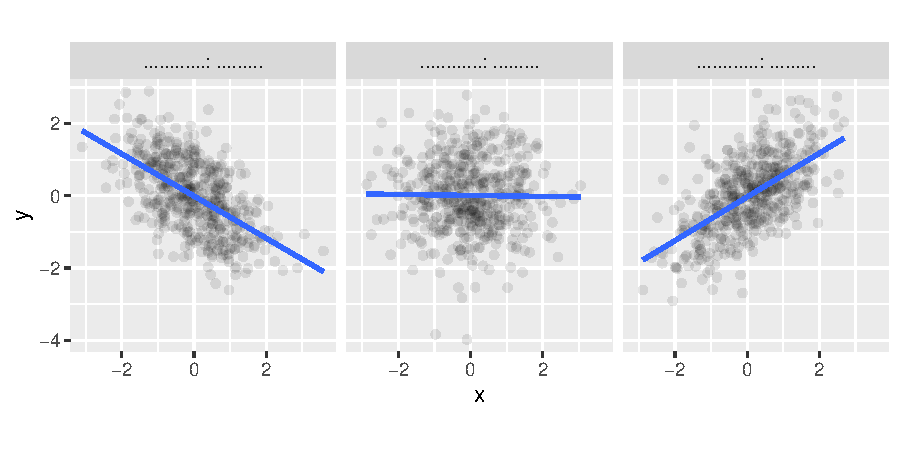
\includegraphics{02-相关和回归_files/figure-latex/correlation-relationships-1.pdf}
\caption{\label{fig:correlation-relationships}不同类型的二元关系}
\end{figure}

如果你有\(n\)个测量值,你可以计算多少个成对相关?你可以用下面蓝框中的公式来计算,也可以更简单地通过R中的\texttt{choose(n,\ 2)}函数直接计算。例如,要获得6个测量值之间可能的成对相关数量,你可以输入\texttt{choose(6,\ 2)},这会告诉你有15对组合。

对于任意\(n\)个测量值,你可以计算\(\frac{n!}{2(n - 2)!}\)个各值之间的成对相关。符号\(!\)称为\textbf{阶乘(factorial)}运算符,定义为从1到\(n\)所有数字的乘积。因此,如果你有6个测量值,你可以得到

\[
\frac{6!}{2(6-2)!} = \frac{1 \times 2 \times 3 \times 4 \times 5 \times 6}{2\left(1 \times 2 \times 3 \times 4\right)} = \frac{720}{2(24)} = 15
\]

你可以使用R中的\texttt{base::cor()}或\texttt{corrr::correlate()}来创建相关矩阵。我们更喜欢后者函数,因为\texttt{cor()}要求你的数据存储在矩阵中,而我们将处理的大多数数据是存储在数据框中的表格数据。\texttt{corrr::correlate()}函数将数据框作为第一个参数,并提供''整洁''的输出,因此它可以更好地与tidyverse系列函数和管道操作符(\texttt{\%\textgreater{}\%})联动。

让我们创建一个相关矩阵来看看它是如何工作的。首先加载我们需要的包。

\begin{Shaded}
\begin{Highlighting}[]
\FunctionTok{library}\NormalTok{(}\StringTok{"tidyverse"}\NormalTok{)}
\FunctionTok{library}\NormalTok{(}\StringTok{"corrr"}\NormalTok{)  }\CommentTok{\# 如缺失(missing),在控制台(console)中输入install.packages("corrr")}
\end{Highlighting}
\end{Shaded}

我们将使用\texttt{starwars}数据集,这是在加载tidyverse包后可用的内置数据集。该数据集包含了出现在星球大战电影系列中的各种角色的信息。让我们来看看之间的相关性

\begin{Shaded}
\begin{Highlighting}[]
\NormalTok{starwars }\SpecialCharTok{\%\textgreater{}\%}
  \FunctionTok{select}\NormalTok{(height, mass, birth\_year) }\SpecialCharTok{\%\textgreater{}\%}
  \FunctionTok{correlate}\NormalTok{()}
\end{Highlighting}
\end{Shaded}

\begin{verbatim}
## Correlation computed with
## * Method: 'pearson'
## * Missing treated using: 'pairwise.complete.obs'
\end{verbatim}

\begin{verbatim}
## # A tibble: 3 x 4
##   term       height   mass birth_year
##   <chr>       <dbl>  <dbl>      <dbl>
## 1 height     NA      0.131     -0.404
## 2 mass        0.131 NA          0.478
## 3 birth_year -0.404  0.478     NA
\end{verbatim}

你可以在任意给定的行或列的交叉处查找任何双变量相关系数。因此,\texttt{height}和\texttt{mass}之间的相关系数是.131,你可以在第1行,第2列或第2行,第1列找到它------它们是相同的。请注意,这里只有\texttt{choose(3,\ 2)} = 3个唯一的双变量关系,但每个关系在表中出现了两次。我们可能只想显示唯一的组合,这可以通过在管道中附加\texttt{corrr::shave()}来实现。

\begin{Shaded}
\begin{Highlighting}[]
\NormalTok{starwars }\SpecialCharTok{\%\textgreater{}\%}
  \FunctionTok{select}\NormalTok{(height, mass, birth\_year) }\SpecialCharTok{\%\textgreater{}\%}
  \FunctionTok{correlate}\NormalTok{() }\SpecialCharTok{\%\textgreater{}\%}
  \FunctionTok{shave}\NormalTok{()}
\end{Highlighting}
\end{Shaded}

\begin{verbatim}
## Correlation computed with
## * Method: 'pearson'
## * Missing treated using: 'pairwise.complete.obs'
\end{verbatim}

\begin{verbatim}
## # A tibble: 3 x 4
##   term       height   mass birth_year
##   <chr>       <dbl>  <dbl>      <dbl>
## 1 height     NA     NA             NA
## 2 mass        0.131 NA             NA
## 3 birth_year -0.404  0.478         NA
\end{verbatim}

现在我们只有相关矩阵的下三角部分,但\texttt{NA}看起来很难看,前导0也不美观。\textbf{\texttt{corrr}}包还提供了\texttt{fashion()}函数,可以对其进行清理(更多选项请查阅\texttt{?corrr::fashion})。

\begin{Shaded}
\begin{Highlighting}[]
\NormalTok{starwars }\SpecialCharTok{\%\textgreater{}\%}
  \FunctionTok{select}\NormalTok{(height, mass, birth\_year) }\SpecialCharTok{\%\textgreater{}\%}
  \FunctionTok{correlate}\NormalTok{() }\SpecialCharTok{\%\textgreater{}\%}
  \FunctionTok{shave}\NormalTok{() }\SpecialCharTok{\%\textgreater{}\%}
  \FunctionTok{fashion}\NormalTok{()}
\end{Highlighting}
\end{Shaded}

\begin{verbatim}
## Correlation computed with
## * Method: 'pearson'
## * Missing treated using: 'pairwise.complete.obs'
\end{verbatim}

\begin{verbatim}
##         term height mass birth_year
## 1     height                       
## 2       mass    .13                
## 3 birth_year   -.40  .48
\end{verbatim}

相关性只有在关系(大致)线性且没有严重的异常值对结果产生过大影响时才能很好地描述关系。因此,可视化相关性通常和量化它们一样是个好主意。\texttt{base::pairs()}函数可以实现这一点。\texttt{pairs()}的第一个参数形式为\texttt{\textasciitilde{}\ v1\ +\ v2\ +\ v3\ +\ ...\ +\ vn},其中\texttt{v1}、\texttt{v2}等是你想要进行相关分析的变量名。

\begin{Shaded}
\begin{Highlighting}[]
\FunctionTok{pairs}\NormalTok{(}\SpecialCharTok{\textasciitilde{}}\NormalTok{ height }\SpecialCharTok{+}\NormalTok{ mass }\SpecialCharTok{+}\NormalTok{ birth\_year, starwars)}
\end{Highlighting}
\end{Shaded}

\begin{figure}
\centering
\includegraphics{02-相关和回归_files/figure-latex/pairs-1.pdf}
\caption{\label{fig:pairs}星球大战数据集相关关系}
\end{figure}

我们会发现一个巨大的离群值影响了我们的数据。具体来说是有个体重超过1200kg的生物。让我们找出它并从数据集里面删掉它。

\begin{Shaded}
\begin{Highlighting}[]
\NormalTok{starwars }\SpecialCharTok{\%\textgreater{}\%}
  \FunctionTok{filter}\NormalTok{(mass }\SpecialCharTok{\textgreater{}} \DecValTok{1200}\NormalTok{) }\SpecialCharTok{\%\textgreater{}\%}
  \FunctionTok{select}\NormalTok{(name, mass, height, birth\_year)}
\end{Highlighting}
\end{Shaded}

\begin{verbatim}
## # A tibble: 1 x 4
##   name                   mass height birth_year
##   <chr>                 <dbl>  <int>      <dbl>
## 1 Jabba Desilijic Tiure  1358    175        600
\end{verbatim}

好了,让我们看看没有了这个庞然大物的数据会是什么样子。

\begin{Shaded}
\begin{Highlighting}[]
\NormalTok{starwars2 }\OtherTok{\textless{}{-}}\NormalTok{ starwars }\SpecialCharTok{\%\textgreater{}\%}
  \FunctionTok{filter}\NormalTok{(name }\SpecialCharTok{!=} \StringTok{"Jabba Desilijic Tiure"}\NormalTok{)}

\FunctionTok{pairs}\NormalTok{(}\SpecialCharTok{\textasciitilde{}}\NormalTok{height }\SpecialCharTok{+}\NormalTok{ mass }\SpecialCharTok{+}\NormalTok{ birth\_year, starwars2)}
\end{Highlighting}
\end{Shaded}

\begin{figure}
\centering
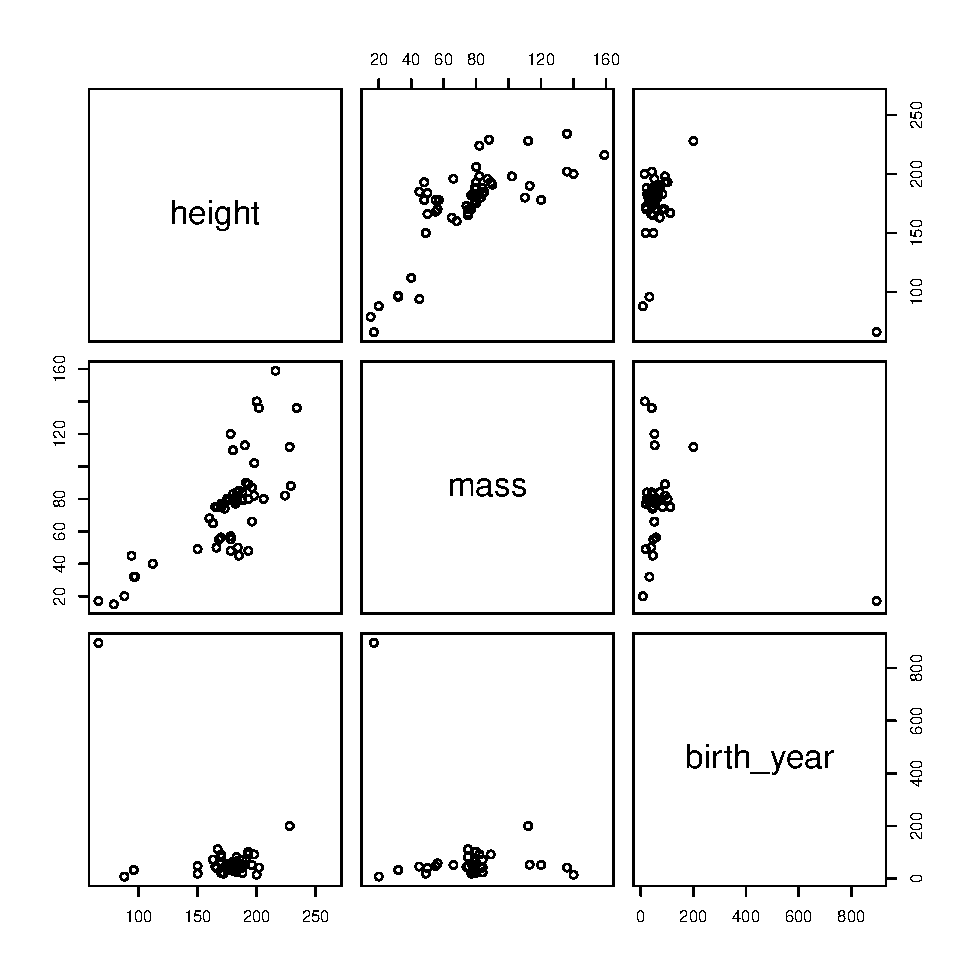
\includegraphics{02-相关和回归_files/figure-latex/massive-creature-1.pdf}
\caption{\label{fig:massive-creature}去除体重离群值后星球大战数据集相关关系}
\end{figure}

好多了,但还有个生物的离群出生年份可能是我们不想要的。

\begin{Shaded}
\begin{Highlighting}[]
\NormalTok{starwars2 }\SpecialCharTok{\%\textgreater{}\%}
  \FunctionTok{filter}\NormalTok{(birth\_year }\SpecialCharTok{\textgreater{}} \DecValTok{800}\NormalTok{) }\SpecialCharTok{\%\textgreater{}\%}
  \FunctionTok{select}\NormalTok{(name, height, mass, birth\_year)}
\end{Highlighting}
\end{Shaded}

\begin{verbatim}
## # A tibble: 1 x 4
##   name  height  mass birth_year
##   <chr>  <int> <dbl>      <dbl>
## 1 Yoda      66    17        896
\end{verbatim}

是尤达大师!他和宇宙一样古老。让我们抛开他看看图会怎么样。

\begin{Shaded}
\begin{Highlighting}[]
\NormalTok{starwars3 }\OtherTok{\textless{}{-}}\NormalTok{ starwars2 }\SpecialCharTok{\%\textgreater{}\%}
  \FunctionTok{filter}\NormalTok{(name }\SpecialCharTok{!=} \StringTok{"Yoda"}\NormalTok{)}

\FunctionTok{pairs}\NormalTok{(}\SpecialCharTok{\textasciitilde{}}\NormalTok{height }\SpecialCharTok{+}\NormalTok{ mass }\SpecialCharTok{+}\NormalTok{ birth\_year, starwars3)}
\end{Highlighting}
\end{Shaded}

\begin{figure}
\centering
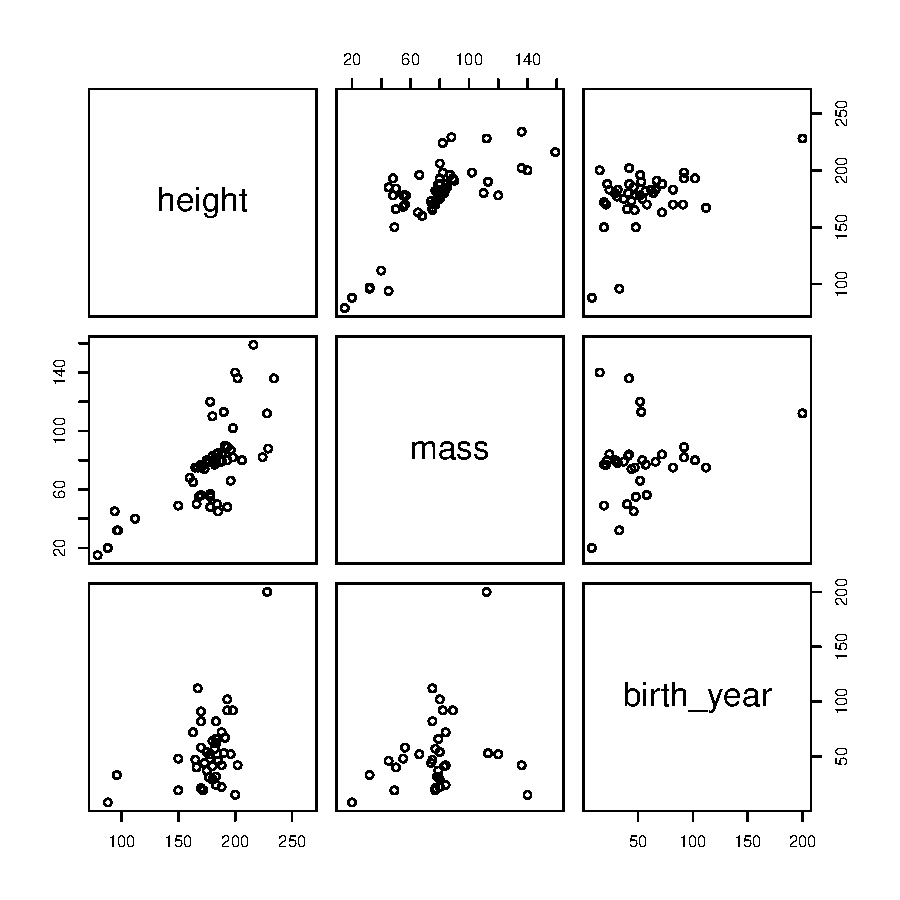
\includegraphics{02-相关和回归_files/figure-latex/bye-yoda-1.pdf}
\caption{\label{fig:bye-yoda}去除体重和出生年份离群值后星球大战数据集相关关系}
\end{figure}

看起来更好了。让我们看看它是怎样改变我们的相关矩阵的。

\begin{Shaded}
\begin{Highlighting}[]
\NormalTok{starwars3 }\SpecialCharTok{\%\textgreater{}\%}
  \FunctionTok{select}\NormalTok{(height, mass, birth\_year) }\SpecialCharTok{\%\textgreater{}\%}
  \FunctionTok{correlate}\NormalTok{() }\SpecialCharTok{\%\textgreater{}\%}
  \FunctionTok{shave}\NormalTok{() }\SpecialCharTok{\%\textgreater{}\%}
  \FunctionTok{fashion}\NormalTok{()}
\end{Highlighting}
\end{Shaded}

\begin{verbatim}
## Correlation computed with
## * Method: 'pearson'
## * Missing treated using: 'pairwise.complete.obs'
\end{verbatim}

\begin{verbatim}
##         term height mass birth_year
## 1     height                       
## 2       mass    .73                
## 3 birth_year    .44  .24
\end{verbatim}

请注意,这些值与我们开始时的值有很大不同。

有时移除离群值不是一个好办法。处理离群值的另一个办法是使用一种更稳健(robust)的方法。使用\texttt{corrr::correlate()}默认计算的相关系数是Pearson积差相关(Pearson product-moment correlation)系数。我们也能通过改变\texttt{correlate()}的\texttt{method()}参数来计算Spearman相关系数。这将在计算相关性之前用排名替换原始值,因此仍会包括离群值,但影响将大大减小。

\begin{Shaded}
\begin{Highlighting}[]
\NormalTok{starwars }\SpecialCharTok{\%\textgreater{}\%}
  \FunctionTok{select}\NormalTok{(height, mass, birth\_year) }\SpecialCharTok{\%\textgreater{}\%}
  \FunctionTok{correlate}\NormalTok{(}\AttributeTok{method =} \StringTok{"spearman"}\NormalTok{) }\SpecialCharTok{\%\textgreater{}\%}
  \FunctionTok{shave}\NormalTok{() }\SpecialCharTok{\%\textgreater{}\%}
  \FunctionTok{fashion}\NormalTok{()}
\end{Highlighting}
\end{Shaded}

\begin{verbatim}
## Correlation computed with
## * Method: 'spearman'
## * Missing treated using: 'pairwise.complete.obs'
\end{verbatim}

\begin{verbatim}
##         term height mass birth_year
## 1     height                       
## 2       mass    .72                
## 3 birth_year    .15  .15
\end{verbatim}

顺便一提,如果你用R Markdown生成报告,并希望你的表格有个好看的格式,可以使用\texttt{knitr::\ able()}。

\begin{Shaded}
\begin{Highlighting}[]
\NormalTok{starwars }\SpecialCharTok{\%\textgreater{}\%}
  \FunctionTok{select}\NormalTok{(height, mass, birth\_year) }\SpecialCharTok{\%\textgreater{}\%}
  \FunctionTok{correlate}\NormalTok{(}\AttributeTok{method =} \StringTok{"spearman"}\NormalTok{) }\SpecialCharTok{\%\textgreater{}\%}
  \FunctionTok{shave}\NormalTok{() }\SpecialCharTok{\%\textgreater{}\%}
  \FunctionTok{fashion}\NormalTok{() }\SpecialCharTok{\%\textgreater{}\%}
\NormalTok{  knitr}\SpecialCharTok{::}\FunctionTok{kable}\NormalTok{()}
\end{Highlighting}
\end{Shaded}

\begin{tabular}{l|l|l|l}
\hline
term & height & mass & birth\_year\\
\hline
height &  &  & \\
\hline
mass & .72 &  & \\
\hline
birth\_year & .15 & .15 & \\
\hline
\end{tabular}

\hypertarget{ux6a21ux62dfux4e8cux5143ux6570ux636e}{%
\section{模拟二元数据}\label{ux6a21ux62dfux4e8cux5143ux6570ux636e}}

你已经学会了使用\texttt{rnorm()}函数从正态分布中模拟数据。回忆一下,\texttt{rnorm()}允许你指定单个变量的均值和标准差。那我们怎么模拟相关变量呢?

应该很明确,你不能仅仅运行两次\texttt{rnorm()}后组合变量就完事。因为这会得到两个不相关的变量,即相关性为零。

\textbf{\texttt{MASS}}包提供\texttt{mvrnorm()}函数,这是rnorm的''多元''(multivariate)版(因此函数的名字是'mv' + `rnorm',这样更容易记住)。

R预装了\textbf{\texttt{MASS}}包。但\textbf{\texttt{MASS}}包中你唯一可能会用到的函数只是\texttt{mvrnorm()},因此相比于使用\texttt{library("MASS")}加载包,使用\texttt{MASS::mvrnorm()}是更好的办法,尤其是在\textbf{\texttt{MASS}}和\textbf{\texttt{tidyverse}}里的\textbf{\texttt{dplyr}}包不太合得来的情况下(因为两个包都有\texttt{select()}函数)。因此,如果在加载\textbf{\texttt{tidyverse}}之后加载\textbf{\texttt{MASS}},那么最终得到的\texttt{select()}是\textbf{\texttt{MASS}}版本,而不是\textbf{\texttt{dplyr}}版本。这会让你绞尽脑汁来找出代码的问题所在,所以总在不加载的情况下使用\texttt{MASS::mvrnorm()}吧。

注:这里作者贴了一则他在Twitter(现X)上吐槽\textbf{\texttt{MASS}}的打油诗,不过现在已经查不到了QwQ,考虑到翻译水平不佳,附上原文!

\begin{quote}
MASS before dplyr, clashes not dire; dplyr before MASS, pain in the ass.

------ Dale Barr(September 30, 2014)
\end{quote}

请查看\texttt{mvrnorm()}函数的文档(在控制台输入\texttt{?MASS::mvrnorm})。

有3个参数需要注意:

\begin{longtable}[]{@{}ll@{}}
\toprule\noalign{}
参数 & 描述 \\
\midrule\noalign{}
\endhead
\bottomrule\noalign{}
\endlastfoot
n & 所需样本数 \\
mu & 一个给出变量均值的向量 \\
Sigma & 一个正定对称矩阵,用于指定变量的协方差矩阵 \\
\end{longtable}

对\texttt{n}和\texttt{mu}的描述可以理解,但``一个正定对称矩阵(positive-definite symmetric matrix),用于指定变量的协方差矩阵''是什么意思呢?

当你有个多层数据时,\textbf{协方差矩阵}(也叫\textbf{方差-协方差矩阵})反映了各个变量的方差及其相互关系。它类似于\textbf{标准差}的多维版本。要充分描述单变量正态分布,你只需要知道均值和标准差;要描述双变量正态分布,你需要分别知道两个变量的均值、标准差和他们的相关性;对于包含两个以上变量的多元分布,你需要知道所有变量的均值、它们的标准差以及所有可能的成对相关性。\textbf{这些概念在我们开始讨论混合效应模型时会变得非常重要。}

你可以将协方差矩阵看作类似于之前见过的相关矩阵;实际上,通过一些计算,你可以将协方差矩阵转换为相关矩阵。

\textbf{你在说什么《黑客帝国(Matrix)》?那不是从上世纪90年代开始的科幻电影系列吗?}

在数学中,矩阵只是向量概念的推广:向量被认为只有一个维度,而矩阵可以是任意数量的维度。

那么矩阵

\[
\begin{pmatrix}
1 & 4 & 7 \\
2 & 5 & 8 \\
3 & 6 & 9 \\
\end{pmatrix}
\]

是一个3(行) x 3(列)矩阵,包括了列向量\(\begin{pmatrix} 1 \\ 2 \\ 3 \\ \end{pmatrix}\),\(\begin{pmatrix} 4 \\ 5 \\ 6 \\ \end{pmatrix}\)和\(\begin{pmatrix} 7 \\ 8 \\ 9 \\ \end{pmatrix}\)。通常我们用\(i\) x \(j\)的形式表示矩阵,\(i\)是行数,\(j\)是列数。因此,一个3x2矩阵有3行2列,像这样:

\[
\begin{pmatrix}
a & d \\
b & e \\
c & f \\
\end{pmatrix}
\]

\textbf{方阵}是行数等于列数的矩阵。

你可以用\texttt{matrix()}函数在R中创建一个方阵,或者使用base R的 \texttt{cbind()}和\texttt{rbind()}将向量连接在一起,它们分别将向量按列和按行连接在一起。在控制台试试\texttt{cbina(1:3,\ 4:6,\ 7:9)}吧。

那么``正定''和``对称''是什么呢?这是对可以表示多元正态分布的这类矩阵的数学要求。换句话说,你提供的协方差矩阵必须表示一个合法的多元正态分布。在这点上,你真的不需要知道再多了。

让我们从模拟假设的人类身高和体重的数据开始。我们知道这些是相关的。为了能够模拟数据,我们需要这两个变量的均值和标准差以及它们的相关性。

我找到了一些\href{https://www.geogebra.org/m/RRprACv4}{数据}并把它转换为CSV文件。如果你想跟上,可以下载这个文件\href{data/heights_and_weights.csv}{heights\_and\_weights.csv}。这是散点图:

\begin{Shaded}
\begin{Highlighting}[]
\NormalTok{handw }\OtherTok{\textless{}{-}} \FunctionTok{read\_csv}\NormalTok{(}\StringTok{"data/heights\_and\_weights.csv"}\NormalTok{, }\AttributeTok{col\_types =} \StringTok{"dd"}\NormalTok{)}

\FunctionTok{ggplot}\NormalTok{(handw, }\FunctionTok{aes}\NormalTok{(height\_in, weight\_lbs)) }\SpecialCharTok{+} 
  \FunctionTok{geom\_point}\NormalTok{(}\AttributeTok{alpha =}\NormalTok{ .}\DecValTok{2}\NormalTok{) }\SpecialCharTok{+}
  \FunctionTok{labs}\NormalTok{(}\AttributeTok{x =} \StringTok{"height (inches)"}\NormalTok{, }\AttributeTok{y =} \StringTok{"weight (pounds)"}\NormalTok{) }
\end{Highlighting}
\end{Shaded}

\begin{figure}
\centering
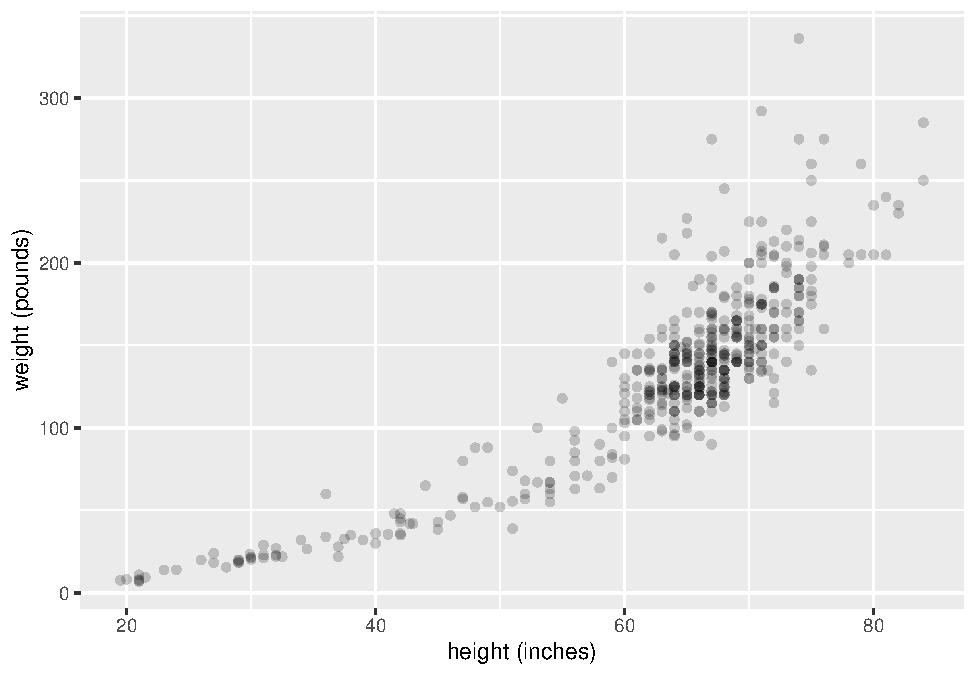
\includegraphics{02-相关和回归_files/figure-latex/heights-and-weights-1.pdf}
\caption{\label{fig:heights-and-weights}475人的身高和体重(包括婴儿)}
\end{figure}

这不是一个线性关系。我们可以先对每个变量进行对数(log)变换。

\begin{Shaded}
\begin{Highlighting}[]
\NormalTok{handw\_log }\OtherTok{\textless{}{-}}\NormalTok{ handw }\SpecialCharTok{\%\textgreater{}\%}
  \FunctionTok{mutate}\NormalTok{(}\AttributeTok{hlog =} \FunctionTok{log}\NormalTok{(height\_in),}
         \AttributeTok{wlog =} \FunctionTok{log}\NormalTok{(weight\_lbs))}
\end{Highlighting}
\end{Shaded}

\begin{figure}
\centering
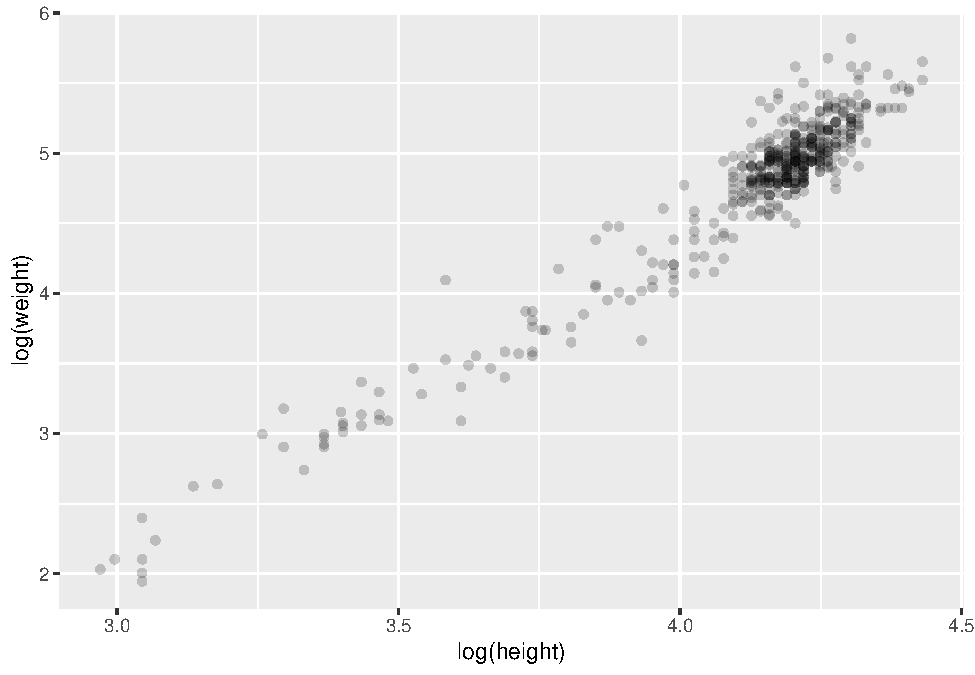
\includegraphics{02-相关和回归_files/figure-latex/handw-log-1.pdf}
\caption{\label{fig:handw-log}对数变换后的身高和体重}
\end{figure}

散点图右上侧尾部有一个大的点簇,这可能表示在这个样本中成年人比儿童更多,因为成年人更高和更重。

对数身高的均值是4.11 (SD = 0.26),而对数体重的均值是4.74 (SD = 0.65)。对数身高和对数体重之间的相关性我们可以用\texttt{cor()}函数获得,高达0.96。

我们现在有了模拟500人身高和体重所需的所有信息。但我们如何将这些信息输入到\texttt{MASS::mvrnorm()}呢?我们知道函数调用的第一部分是\texttt{MASS::mvrnorm(500,\ c(4.11,4.74),\ ...)},但\texttt{Sigma}------那个协方差矩阵呢?我们从上面知道\(\hat{\sigma}_x = 0.26\)和\(\hat{\sigma}_y = 0.65\),以及\(\hat{\sigma}_y = 0.65\), and \(\hat{\rho}_{xy} = 0.96\)。

表示二元数据\texttt{Sigma} (\(\mathbf{\Sigma}\))的协方差矩阵如下:

\[
\mathbf{\Sigma} =
\begin{pmatrix}
{\sigma_x}^2                & \rho_{xy} \sigma_x \sigma_y \\
\rho_{yx} \sigma_y \sigma_x & {\sigma_y}^2 \\
\end{pmatrix}
\]

方差(标准差的平方,\({\sigma_x}^2\)和\({\sigma_y}^2\))位于对角线上,协方差(相关系数乘以两个标准差,\(\rho_{xy} \sigma_x \sigma_y\))位于非对角线上。记住协方差就是相关系数与两个标准差的积,这是很有用的。正如我们在上面的相关矩阵中看到的,表格中存在额外信息;也就是说,协方差同时出现在矩阵的右上角单元格和左下角单元格。

代入之前的值,协方差矩阵应该是:

\[
\begin{pmatrix}
.26^2 & (.96)(.26)(.65) \\
(.96)(.65)(.26) & .65^2 \\
\end{pmatrix} =
\begin{pmatrix}
.067 & .162 \\
.162 & .423 \\
\end{pmatrix}
\]

很好,那么我们如何在R中形成\texttt{Sigma}以便我们可以将它传递给\texttt{mvrnorm()}函数呢?我们将使用\texttt{matrix()}函数,如下所示。

首先,让我们定义协方差并将其存储在变量\texttt{my\_cov}中。

\begin{Shaded}
\begin{Highlighting}[]
\NormalTok{my\_cov }\OtherTok{\textless{}{-}}\NormalTok{ .}\DecValTok{96} \SpecialCharTok{*}\NormalTok{ .}\DecValTok{26} \SpecialCharTok{*}\NormalTok{ .}\DecValTok{65}
\end{Highlighting}
\end{Shaded}

现在我们将使用\texttt{matrix()}来定义我们的\texttt{Sigma}为\texttt{my\_Sigma}。

\begin{Shaded}
\begin{Highlighting}[]
\NormalTok{my\_Sigma }\OtherTok{\textless{}{-}} \FunctionTok{matrix}\NormalTok{(}\FunctionTok{c}\NormalTok{(.}\DecValTok{26}\SpecialCharTok{\^{}}\DecValTok{2}\NormalTok{, my\_cov, my\_cov, .}\DecValTok{65}\SpecialCharTok{\^{}}\DecValTok{2}\NormalTok{), }\AttributeTok{ncol =} \DecValTok{2}\NormalTok{)}
\NormalTok{my\_Sigma}
\end{Highlighting}
\end{Shaded}

\begin{verbatim}
##         [,1]    [,2]
## [1,] 0.06760 0.16224
## [2,] 0.16224 0.42250
\end{verbatim}

\textbf{对\texttt{matrix()}函数感到困惑吗?}

通过运行下面的代码,你可以发现\texttt{matrix()}是逐列填充矩阵元素,而不是逐行填充:

\texttt{matrix(c("a",\ "b",\ "c",\ "d"),\ ncol\ =\ 2)}

如果你想改变这种行为,将\texttt{byrow}参数设置为\texttt{TRUE}。

\texttt{matrix(c("a",\ "b",\ "c",\ "d"),\ ncol\ =\ 2,\ byrow\ =\ TRUE)}

太好了!现在我们得到了\texttt{my\_Sigma},我们已经准备好使用\texttt{MASS::mvrnorm()}了。让我们通过创建6个模拟的人的数据来测试一下。

\begin{Shaded}
\begin{Highlighting}[]
\FunctionTok{set.seed}\NormalTok{(}\DecValTok{62}\NormalTok{) }\CommentTok{\# 为了可重复性}

\CommentTok{\# 传递*命名的*向量c(height = 4.11, weight = 4.74)给mu可以在输出中得到列名}
\NormalTok{log\_ht\_wt }\OtherTok{\textless{}{-}}\NormalTok{ MASS}\SpecialCharTok{::}\FunctionTok{mvrnorm}\NormalTok{(}\DecValTok{6}\NormalTok{, }
                           \FunctionTok{c}\NormalTok{(}\AttributeTok{height =} \FloatTok{4.11}\NormalTok{, }\AttributeTok{weight =} \FloatTok{4.74}\NormalTok{), }
\NormalTok{                           my\_Sigma)}

\NormalTok{log\_ht\_wt}
\end{Highlighting}
\end{Shaded}

\begin{verbatim}
##        height   weight
## [1,] 4.254209 5.282913
## [2,] 4.257828 4.895222
## [3,] 3.722376 3.759767
## [4,] 4.191287 4.764229
## [5,] 4.739967 6.185191
## [6,] 4.058105 4.806485
\end{verbatim}

那么\texttt{MASS::mvrnorm()}会返回一个矩阵,每个模拟的人对应一行,其中第一列表示对数身高,第二列表示对数体重。但是对数身高和对数体重对我们来说并不是很有用,所以让我们使用\texttt{exp()}函数来进行转换,它是\texttt{log()}转换的逆操作。

\begin{Shaded}
\begin{Highlighting}[]
\FunctionTok{exp}\NormalTok{(log\_ht\_wt)}
\end{Highlighting}
\end{Shaded}

\begin{verbatim}
##         height    weight
## [1,]  70.40108 196.94276
## [2,]  70.65632 133.64963
## [3,]  41.36254  42.93844
## [4,]  66.10779 117.24065
## [5,] 114.43045 485.50576
## [6,]  57.86453 122.30092
\end{verbatim}

那么我们第一个模拟的人的身高是70.4英寸(大约是5'5''或者178.816 cm),体重是196.94磅(约89.32 kg)。听起来感觉不错吧!(还是要注意,它会生成超出我们原始数据范围的观测值:我们会得到超高的人,例如第5个观测值,但至少体重/身高的关系会被保留)。

好的,让我们随机生成一群人的数据,将它们从对数转换为英寸和磅,然后将它们与我们的原始数据进行比较,看看效果如何。

\begin{Shaded}
\begin{Highlighting}[]
\DocumentationTok{\#\# 模拟新的人}
\NormalTok{new\_humans }\OtherTok{\textless{}{-}}\NormalTok{ MASS}\SpecialCharTok{::}\FunctionTok{mvrnorm}\NormalTok{(}\DecValTok{500}\NormalTok{, }
                            \FunctionTok{c}\NormalTok{(}\AttributeTok{height\_in =} \FloatTok{4.11}\NormalTok{, }\AttributeTok{weight\_lbs =} \FloatTok{4.74}\NormalTok{),}
\NormalTok{                            my\_Sigma) }\SpecialCharTok{\%\textgreater{}\%}
  \FunctionTok{exp}\NormalTok{() }\SpecialCharTok{\%\textgreater{}\%} \CommentTok{\# 从对数转换回英寸和磅}
  \FunctionTok{as\_tibble}\NormalTok{() }\SpecialCharTok{\%\textgreater{}\%} \CommentTok{\# 为绘图转换为tibble格式}
  \FunctionTok{mutate}\NormalTok{(}\AttributeTok{type =} \StringTok{"simulated"}\NormalTok{) }\CommentTok{\# 将他们标记为模拟(simulated)}

\DocumentationTok{\#\# 合并真实和模拟的数据集,其中handw是来自heights\_and\_weights.csv的变量}
\NormalTok{alldata }\OtherTok{\textless{}{-}} \FunctionTok{bind\_rows}\NormalTok{(handw }\SpecialCharTok{\%\textgreater{}\%} \FunctionTok{mutate}\NormalTok{(}\AttributeTok{type =} \StringTok{"real"}\NormalTok{), }
\NormalTok{                     new\_humans)}

\FunctionTok{ggplot}\NormalTok{(alldata, }\FunctionTok{aes}\NormalTok{(height\_in, weight\_lbs)) }\SpecialCharTok{+}
  \FunctionTok{geom\_point}\NormalTok{(}\FunctionTok{aes}\NormalTok{(}\AttributeTok{colour =}\NormalTok{ type), }\AttributeTok{alpha =}\NormalTok{ .}\DecValTok{1}\NormalTok{)}
\end{Highlighting}
\end{Shaded}

\begin{figure}
\centering
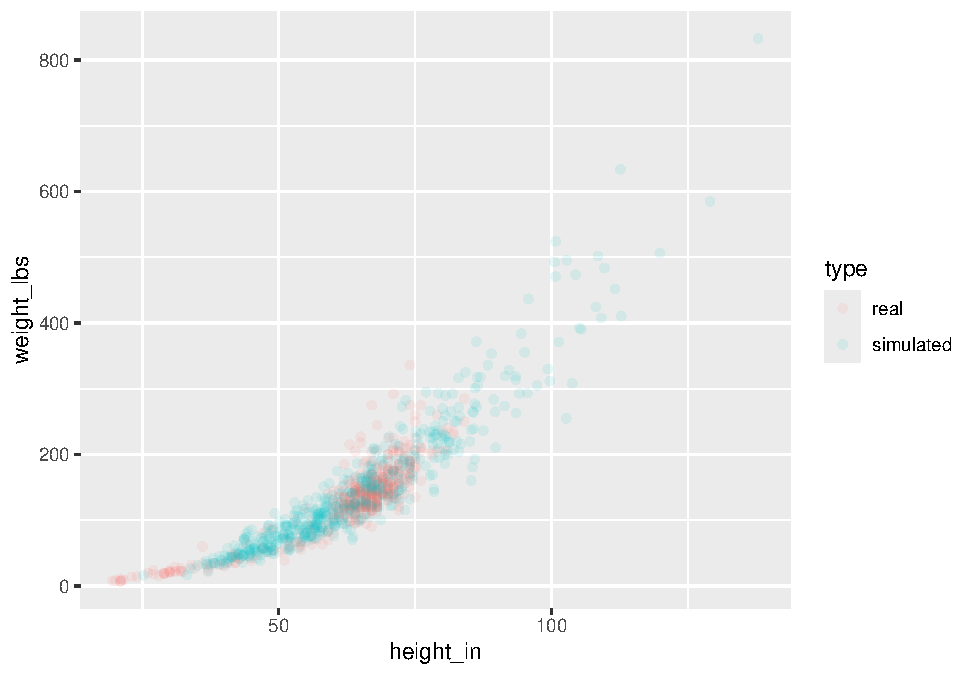
\includegraphics{02-相关和回归_files/figure-latex/plot-together-1.pdf}
\caption{\label{fig:plot-together}真实和模拟的人}
\end{figure}

你可以看到,我们模拟的人与正常的人非常相似,只是我们创建了一些身高和体重超出正常范围的人。

\hypertarget{ux76f8ux5173ux548cux56deux5f52ux7684ux5173ux7cfb}{%
\section{相关和回归的关系}\label{ux76f8ux5173ux548cux56deux5f52ux7684ux5173ux7cfb}}

好的,我们知道如何估计相关了,但如果我们想要根据身高来预测体重该怎么办呢?这可能听起来像一个不切实际的问题。但事实上,在使用或进行安全性取决于患者体重的药物或程序,但没时间称量患者体重时,\href{https://link.springer.com/article/10.1186/s12245-018-0212-9}{急救医护人员可以使用这种技术,在紧急情况下迅速估算人们的体重}。

回忆一下,简单回归模型的GLM是:

\[Y_i = \beta_0 + \beta_1 X_i + e_i.\]

在这里,我们尝试根据他们观测到的身高(\(X_i\))来预测体重(\(Y_i\))。在这个方程里,\(\beta_0\)和\(\beta_1\)分别是y轴截距和斜率的参数,\(e_i\)是残差。传统上假设\(e_i\)的值来自均值为0、方差为\(\sigma^2\)的正态分布;数学上的表述是\(e_i \sim N(0, \sigma^2)\),其中\(\sim\)表示``按照分布'',\(N(0, \sigma^2)\)表示``均值为0、方差为\(\sigma^2\)的正态分布(\(N\))''。

这表明如果我们有X和Y的均值估计值(分别标记为\(\mu_x\)和\(\mu_y\))、标准差估计值(\(\hat{\sigma}_x\)和\(\hat{\sigma}_y\))、X和Y之间相关系数的估计值(\(\hat{\rho}\)),我们就有了估计回归方程参数\(\beta_0\)和\(\beta_1\)所需要的所有信息。下面是具体做法。(译者注:这里的估计值是指根据样本信息来估计总体情况的估计值,是总体的估计值、样本的观测值)

首先,回归线的斜率\(\beta_1\)等于相关系数\(\rho\)乘以\(Y\)和\(X\)的标准差之比。

\[\beta_1 = \rho \frac{\sigma_Y}{\sigma_X}\]

根据上面对数身高和对数体重的估计值,你能算出\(\beta_1\)吗?

\begin{Shaded}
\begin{Highlighting}[]
\NormalTok{b1 }\OtherTok{\textless{}{-}}\NormalTok{ .}\DecValTok{96} \SpecialCharTok{*}\NormalTok{ (.}\DecValTok{65} \SpecialCharTok{/}\NormalTok{ .}\DecValTok{26}\NormalTok{)}
\NormalTok{b1}
\end{Highlighting}
\end{Shaded}

\begin{verbatim}
## [1] 2.4
\end{verbatim}

下一个要注意的点是,基于数学原理,回归线必须通过与\(X\)和\(Y\)均值对应的点,即点\((\mu_x, \mu_y)\)(你可以想象回归线根据斜率围绕该点``旋转'')。你也知道\(\beta_0\)是y轴截距,即在\(X = 0\)处与纵轴相交的点。根据这些信息和上面的估计值,你能推断出\(\beta_0\)的值吗?

下面是你求解\(\beta_0\)的推理过程。

想象一下,从\(X = \mu_x\)逐步一个一个单位后退到\(X = 0\)。在\(X = \mu_x\)处,\(Y = 4.74\),每在X轴后退一个单位,\(Y\)将下降\(\beta_1 = 2.4\)个单位。当你到0时,\(Y\)将从\(\mu_y\)下降到\(\mu_y - \mu_x \beta_1\)。

因此通解是:\(\beta_0 = \mu_y - \mu_x\beta_1\)。

因为\(\beta_1 = 2.4\)、\(\mu_x = 4.11\)、\(\mu_y = 4.74\),所以\(\beta_0 = -5.124\)。因此,我们的回归方程是:

\[Y_i =  -5.124 + 2.4X_i + e_i.\]

为了验证我们的结果,我们先对对数转换后的数据进行回归,使用\texttt{lm()}函数,它采用最小二乘法(ordinary least squares regression)来估计参数。

\begin{Shaded}
\begin{Highlighting}[]
\FunctionTok{summary}\NormalTok{(}\FunctionTok{lm}\NormalTok{(wlog }\SpecialCharTok{\textasciitilde{}}\NormalTok{ hlog, handw\_log))}
\end{Highlighting}
\end{Shaded}

\begin{verbatim}
## 
## Call:
## lm(formula = wlog ~ hlog, data = handw_log)
## 
## Residuals:
##      Min       1Q   Median       3Q      Max 
## -0.63296 -0.09915 -0.01366  0.09285  0.65635 
## 
## Coefficients:
##             Estimate Std. Error t value Pr(>|t|)    
## (Intercept) -5.26977    0.13169  -40.02   <2e-16 ***
## hlog         2.43304    0.03194   76.17   <2e-16 ***
## ---
## Signif. codes:  0 '***' 0.001 '**' 0.01 '*' 0.05 '.' 0.1 ' ' 1
## 
## Residual standard error: 0.1774 on 473 degrees of freedom
## Multiple R-squared:  0.9246, Adjusted R-squared:  0.9245 
## F-statistic:  5802 on 1 and 473 DF,  p-value: < 2.2e-16
\end{verbatim}

看起来非常接近。不完全匹配的原因仅仅是我们将估计值四舍五入到小数点后两位以方便计算。

作为另一个检查,让我们将手动计算的回归线叠加在对数转换后数据的散点图上。

\begin{Shaded}
\begin{Highlighting}[]
\FunctionTok{ggplot}\NormalTok{(handw\_log, }\FunctionTok{aes}\NormalTok{(hlog, wlog)) }\SpecialCharTok{+}
  \FunctionTok{geom\_point}\NormalTok{(}\AttributeTok{alpha =}\NormalTok{ .}\DecValTok{2}\NormalTok{) }\SpecialCharTok{+}
  \FunctionTok{labs}\NormalTok{(}\AttributeTok{x =} \StringTok{"log(height)"}\NormalTok{, }\AttributeTok{y =} \StringTok{"log(weight)"}\NormalTok{) }\SpecialCharTok{+}
  \FunctionTok{geom\_abline}\NormalTok{(}\AttributeTok{intercept =} \SpecialCharTok{{-}}\FloatTok{5.124}\NormalTok{, }\AttributeTok{slope =} \FloatTok{2.4}\NormalTok{, }\AttributeTok{colour =} \StringTok{\textquotesingle{}blue\textquotesingle{}}\NormalTok{)}
\end{Highlighting}
\end{Shaded}

\begin{figure}
\centering
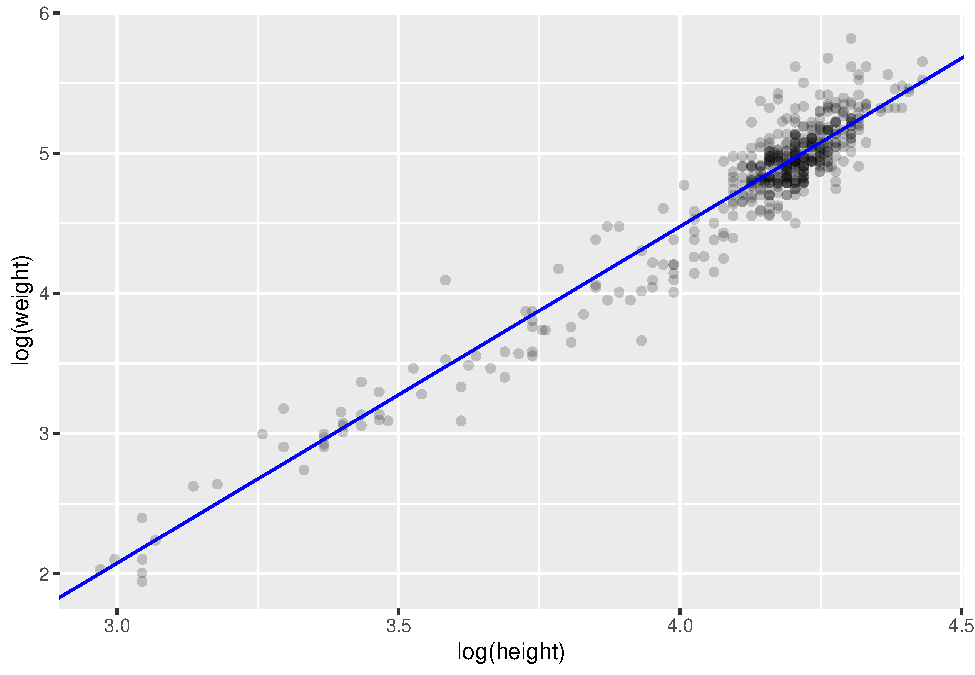
\includegraphics{02-相关和回归_files/figure-latex/scatter-with-line-1.pdf}
\caption{\label{fig:scatter-with-line}对数值和叠加的回归线}
\end{figure}

看起来是对的。

最后,以下是相关性和回归之间关系的一些影响:

\begin{itemize}
\tightlist
\item
  当\(\beta_1 = 0\)时,与\(\rho = 0\)相同。
\item
  当\(\beta_1 > 0\)时, \(\rho > 0\),因为标准差不能为负。
\item
  当\(\beta_1 < 0\)时, \(\rho < 0\),原因同上。
\item
  拒绝零假设\(\beta_1 = 0\)与拒绝零假设\(\rho = 0\)是相同的。在\texttt{lm()}中得到的\(\beta_1\)的p值与使用\texttt{cor.test()}得到的\(\rho\)的p值相同。
\end{itemize}

\hypertarget{ux7ec3ux4e60}{%
\section{练习}\label{ux7ec3ux4e60}}

\hypertarget{ux591aux5143ux56deux5f52}{%
\chapter{多元回归}\label{ux591aux5143ux56deux5f52}}

单层数据包含\(m\)个预测变量的一般模型是:

\[
Y_i = \beta_0 + \beta_1 X_{1i} + \beta_2 X_{2i} + \ldots + \beta_m X_{mi} + e_i
\]

其中\(e_i \sim \mathcal{N}\left(0, \sigma^2\right)\),换句话说,我们假设误差来自一个均值为0,方差为\(\sigma^2\)的正态分布。

注意,这里的关键假设\textbf{不是}响应变量(\(Y\))服从正态分布,\textbf{也不是}单个预测变量(\(X\))服从正态分布;而是\textbf{仅}模型残差服从正态分布(详细讨论见这篇\href{https://datahowler.wordpress.com/2018/08/04/checking-model-assumptions-look-at-the-residuals-not-the-raw-data/}{博客})。单个\(X\)预测变量可以是任意组合的连续变量和/或分类变量,包括变量之间的交互。这个特定模型背后的进一步假设是,关系是''平面的''(可以用一个平面描述,类似于简单回归中的线性假设),且误差方差与预测变量无关。

\(\beta\)的值被称为\textbf{回归系数(regression coefficient)}。每个\(\beta_h\)被解释为\textbf{在保持其他所有预测变量不变的情况下}\(\beta_h\)的偏效应(partial effect)。如果你有\(m\)个预测变量,你将有\(m+1\)个回归系数:一个用于截距,每个预测变量各一个

尽管在统计教科书中对多元回归的讨论很常见,但你很少有机会应用到上述的精确模型。因为上述模型假设的是单层数据,而大多数心理学数据是多层的。然而,这两种数据集的基本原理是相同的,因此先学习比较简单的案例是值得的。

\hypertarget{ux4e00ux4e2aux4f8bux5b50ux5982ux4f55ux5728ux7edfux8ba1ux5b66ux4e0aux53d6ux5f97ux597dux6210ux7ee9}{%
\section{一个例子:如何在统计学上取得好成绩}\label{ux4e00ux4e2aux4f8bux5b50ux5982ux4f55ux5728ux7edfux8ba1ux5b66ux4e0aux53d6ux5f97ux597dux6210ux7ee9}}

让我们来看一些(虚构但基于现实的)数据,看看我们如何使用多元回归来回答各种研究问题。在这个假设的研究中,你有一个包含100名统计学学生的数据集,其中包括他们的最终课程成绩(\texttt{grade})、每个学生参加讲座的次数(\texttt{lecture},一个范围为0-10的整数)、每个学生点击下载在线资料的次数(\texttt{nclicks})以及每个学生在修这门课程之前的平均绩点(\texttt{GPA}),其范围从0(不及格)到4(最高可能成绩)。

\hypertarget{ux6570ux636eux5bfcux5165ux548cux53efux89c6ux5316}{%
\subsection{数据导入和可视化}\label{ux6570ux636eux5bfcux5165ux548cux53efux89c6ux5316}}

让我们加载数据\href{https://raw.githubusercontent.com/PsyTeachR/stat-models-v1/master/data/grades.csv}{grades.csv}并看一看。

\begin{Shaded}
\begin{Highlighting}[]
\FunctionTok{library}\NormalTok{(}\StringTok{"corrr"}\NormalTok{) }\CommentTok{\# 相关矩阵}
\FunctionTok{library}\NormalTok{(}\StringTok{"tidyverse"}\NormalTok{)}

\NormalTok{grades }\OtherTok{\textless{}{-}} \FunctionTok{read\_csv}\NormalTok{(}\StringTok{"data/grades.csv"}\NormalTok{, }\AttributeTok{col\_types =} \StringTok{"ddii"}\NormalTok{)}

\NormalTok{grades}
\end{Highlighting}
\end{Shaded}

\begin{verbatim}
## # A tibble: 100 x 4
##    grade   GPA lecture nclicks
##    <dbl> <dbl>   <int>   <int>
##  1  2.40 1.13        6      88
##  2  3.67 0.971       6      96
##  3  2.85 3.34        6     123
##  4  1.36 2.76        9      99
##  5  2.31 1.02        4      66
##  6  2.58 0.841       8      99
##  7  2.69 4           5      86
##  8  3.05 2.29        7     118
##  9  3.21 3.39        9      98
## 10  2.24 3.27       10     115
## # i 90 more rows
\end{verbatim}

首先,让我们看一看所有的两两相关。

\begin{Shaded}
\begin{Highlighting}[]
\NormalTok{grades }\SpecialCharTok{\%\textgreater{}\%}
  \FunctionTok{correlate}\NormalTok{() }\SpecialCharTok{\%\textgreater{}\%}
  \FunctionTok{shave}\NormalTok{() }\SpecialCharTok{\%\textgreater{}\%}
  \FunctionTok{fashion}\NormalTok{()}
\end{Highlighting}
\end{Shaded}

\begin{verbatim}
## Correlation computed with
## * Method: 'pearson'
## * Missing treated using: 'pairwise.complete.obs'
\end{verbatim}

\begin{verbatim}
##      term grade  GPA lecture nclicks
## 1   grade                           
## 2     GPA   .25                     
## 3 lecture   .24  .44                
## 4 nclicks   .16  .30     .36
\end{verbatim}

\begin{Shaded}
\begin{Highlighting}[]
\FunctionTok{pairs}\NormalTok{(grades)}
\end{Highlighting}
\end{Shaded}

\begin{figure}
\centering
\includegraphics{03-多元回归_files/figure-latex/pairs-1.pdf}
\caption{\label{fig:pairs}\texttt{grades}数据集中的所有成对关系}
\end{figure}

\hypertarget{ux4f30ux8ba1ux548cux89e3ux91ca}{%
\subsection{估计和解释}\label{ux4f30ux8ba1ux548cux89e3ux91ca}}

我们将使用\texttt{lm()}函数来估计回归系数(\(\beta\)s)。针对一个有\(m\)个预测变量的GLM:

\[
Y_i = \beta_0 + \beta_1 X_{1i} + \beta_2 X_{2i} + \ldots + \beta_m X_{mi} + e_i
\]

对base R的\texttt{lm()}调用如下:

\texttt{lm(Y\ \textasciitilde{}\ X1\ +\ X2\ +\ ...\ +\ Xm,\ data)}

变量\texttt{Y}是你的响应变量,变量\texttt{X}是预测变量。注意,你不需要明确指定截距或残差项;这些是默认包含的。

对于当前数据,让我们通过\texttt{lecture}和\texttt{nclicks}来预测\texttt{grade}。

\begin{Shaded}
\begin{Highlighting}[]
\NormalTok{my\_model }\OtherTok{\textless{}{-}} \FunctionTok{lm}\NormalTok{(grade }\SpecialCharTok{\textasciitilde{}}\NormalTok{ lecture }\SpecialCharTok{+}\NormalTok{ nclicks, grades)}

\FunctionTok{summary}\NormalTok{(my\_model)}
\end{Highlighting}
\end{Shaded}

\begin{verbatim}
## 
## Call:
## lm(formula = grade ~ lecture + nclicks, data = grades)
## 
## Residuals:
##      Min       1Q   Median       3Q      Max 
## -2.21653 -0.40603  0.02267  0.60720  1.38558 
## 
## Coefficients:
##             Estimate Std. Error t value Pr(>|t|)  
## (Intercept) 1.462037   0.571124   2.560   0.0120 *
## lecture     0.091501   0.045766   1.999   0.0484 *
## nclicks     0.005052   0.006051   0.835   0.4058  
## ---
## Signif. codes:  0 '***' 0.001 '**' 0.01 '*' 0.05 '.' 0.1 ' ' 1
## 
## Residual standard error: 0.8692 on 97 degrees of freedom
## Multiple R-squared:  0.06543,    Adjusted R-squared:  0.04616 
## F-statistic: 3.395 on 2 and 97 DF,  p-value: 0.03756
\end{verbatim}

我们通常会在参数符号的顶部加上一个帽子(hat),以明确我们正在处理样本的估计值,而不是(未知的)真实总体值。由上可知:

\begin{itemize}
\tightlist
\item
  \(\hat{\beta}_0\) = 1.46
\item
  \(\hat{\beta}_1\) = 0.09
\item
  \(\hat{\beta}_2\) = 0.01
\end{itemize}

这告诉我们,一个人的预期成绩与他们的参加讲座的次数和点击下载在线资料的次数通过以下公式相关联:

\texttt{grade} = 1.46 + 0.09 \(\times\) \texttt{lecture} + 0.01 \(\times\) \texttt{nclicks}

因为\(\hat{\beta}_1\)和\(\hat{\beta}_2\)都是正数,所以我们知道\texttt{lecture}和\texttt{nclicks}的值越高,成绩越好。

因此,如果有人问你,你预测一个参加了3次讲座并下载了70次的学生成绩是多少,你可以通过代入相应的值轻松算出来。

\texttt{grade} = 1.46 + 0.09 \(\times\) 3 + 0.01 \(\times\) 70

相当于:

\texttt{grade} = 1.46 + 0.27 + 0.7

可化简为:

\texttt{grade} = 2.43

\hypertarget{ux4f7fux7528predictux901aux8fc7ux7ebfux6027ux6a21ux578bux8fdbux884cux9884ux6d4b}{%
\subsection{\texorpdfstring{使用\texttt{predict()}通过线性模型进行预测}{使用predict()通过线性模型进行预测}}\label{ux4f7fux7528predictux901aux8fc7ux7ebfux6027ux6a21ux578bux8fdbux884cux9884ux6d4b}}

如果我们想通过新的预测变量值来预测响应变量值,我们可以使用base R 的\texttt{predict()}函数。

\texttt{predict()}函数有两个主要参数。第一个参数是拟合的模型对象(即上面的my\_model),第二个参数是包含预测变量新值的数据框(或tibble,R中和数据框data frame类似的一种数据格式)。

在新表中,你需要包含\textbf{所有的}预测变量。如果您的tibble缺少任何预测变量,你将收到错误消息(error message)。您还需要确保新表中的变量名与模型中的变量名\textbf{完全}匹配。

让我们创建一个带有新值的tibble并进行测试。

\begin{Shaded}
\begin{Highlighting}[]
\DocumentationTok{\#\# “tribble”是一种按行而不是按列创建tibble的方法。有时这样做会很有用。}
\NormalTok{new\_data }\OtherTok{\textless{}{-}} \FunctionTok{tribble}\NormalTok{(}\SpecialCharTok{\textasciitilde{}}\NormalTok{lecture, }\SpecialCharTok{\textasciitilde{}}\NormalTok{nclicks,}
                    \DecValTok{3}\NormalTok{, }\DecValTok{70}\NormalTok{,}
                    \DecValTok{10}\NormalTok{, }\DecValTok{130}\NormalTok{,}
                    \DecValTok{0}\NormalTok{, }\DecValTok{20}\NormalTok{,}
                    \DecValTok{5}\NormalTok{, }\DecValTok{100}\NormalTok{)}
\end{Highlighting}
\end{Shaded}

\texttt{tribble()}函数提供了一种按行而不是按列逐步构建tibble的方法,而使用\texttt{tibble()}函数则是按列逐步构建表格。

\texttt{tribble()}的第一行包含列名,每个列名前面都有一个波浪号(\texttt{\textasciitilde{}})。

有时这种方法比逐行构建更容易阅读,尽管结果是相同的。考虑到这些,我们也可以使用以下方式创建上述表格:

\begin{Shaded}
\begin{Highlighting}[]
\NormalTok{new\_data }\OtherTok{\textless{}{-}} \FunctionTok{tibble}\NormalTok{(}\AttributeTok{lecture =} \FunctionTok{c}\NormalTok{(}\DecValTok{3}\NormalTok{, }\DecValTok{10}\NormalTok{, }\DecValTok{0}\NormalTok{, }\DecValTok{5}\NormalTok{),}
                   \AttributeTok{nclicks =} \FunctionTok{c}\NormalTok{(}\DecValTok{70}\NormalTok{, }\DecValTok{130}\NormalTok{, }\DecValTok{20}\NormalTok{, }\DecValTok{100}\NormalTok{))}
\end{Highlighting}
\end{Shaded}

现在我们已经创建了表\texttt{new\_data},只需将其传递给\texttt{predict()}函数,这会返回一个关于\(Y\)(grade)预测值的向量。

\begin{Shaded}
\begin{Highlighting}[]
\FunctionTok{predict}\NormalTok{(my\_model, new\_data)}
\end{Highlighting}
\end{Shaded}

\begin{verbatim}
##        1        2        3        4 
## 2.090214 3.033869 1.563087 2.424790
\end{verbatim}

这很好,但也许我们希望将预测值和预测变量对应起来。我们可以通过将预测值作为新列添加到\texttt{new\_data}中来实现这一点。

\begin{Shaded}
\begin{Highlighting}[]
\NormalTok{new\_data }\SpecialCharTok{\%\textgreater{}\%}
  \FunctionTok{mutate}\NormalTok{(}\AttributeTok{predicted\_grade =} \FunctionTok{predict}\NormalTok{(my\_model, new\_data))}
\end{Highlighting}
\end{Shaded}

\begin{verbatim}
## # A tibble: 4 x 3
##   lecture nclicks predicted_grade
##     <dbl>   <dbl>           <dbl>
## 1       3      70            2.09
## 2      10     130            3.03
## 3       0      20            1.56
## 4       5     100            2.42
\end{verbatim}

想查看\texttt{predict()}的更多操作吗?使用\texttt{?predict.lm}来获得帮助。

\hypertarget{ux504fux6548ux5e94ux53efux89c6ux5316}{%
\subsection{偏效应可视化}\label{ux504fux6548ux5e94ux53efux89c6ux5316}}

如上所述,每个回归系数的参数估计值告诉我们该变量的\textbf{偏}效应;即保持其他所有变量不变时它的效应。有办法可视化这个偏效应吗?是的,你可以使用\texttt{predict()}函数来实现,通过创建一个表,其中焦点预测变量(focal predictor)的值是多样的,其他所有预测变量用均值填充。

例如,我们要可视化\texttt{lecture}对\texttt{grade}的偏效应,同时将\texttt{nclicks}的值保持在其均值不变。

\begin{Shaded}
\begin{Highlighting}[]
\NormalTok{nclicks\_mean }\OtherTok{\textless{}{-}}\NormalTok{ grades }\SpecialCharTok{\%\textgreater{}\%} \FunctionTok{pull}\NormalTok{(nclicks) }\SpecialCharTok{\%\textgreater{}\%} \FunctionTok{mean}\NormalTok{()}

\DocumentationTok{\#\# 预测用的新数据}
\NormalTok{new\_lecture }\OtherTok{\textless{}{-}} \FunctionTok{tibble}\NormalTok{(}\AttributeTok{lecture =} \DecValTok{0}\SpecialCharTok{:}\DecValTok{10}\NormalTok{,}
                      \AttributeTok{nclicks =}\NormalTok{ nclicks\_mean)}

\DocumentationTok{\#\# 将预测值添加到new\_lecture}
\NormalTok{new\_lecture2 }\OtherTok{\textless{}{-}}\NormalTok{ new\_lecture }\SpecialCharTok{\%\textgreater{}\%}
  \FunctionTok{mutate}\NormalTok{(}\AttributeTok{grade =} \FunctionTok{predict}\NormalTok{(my\_model, new\_lecture))}

\NormalTok{new\_lecture2}
\end{Highlighting}
\end{Shaded}

\begin{verbatim}
## # A tibble: 11 x 3
##    lecture nclicks grade
##      <int>   <dbl> <dbl>
##  1       0    98.3  1.96
##  2       1    98.3  2.05
##  3       2    98.3  2.14
##  4       3    98.3  2.23
##  5       4    98.3  2.32
##  6       5    98.3  2.42
##  7       6    98.3  2.51
##  8       7    98.3  2.60
##  9       8    98.3  2.69
## 10       9    98.3  2.78
## 11      10    98.3  2.87
\end{verbatim}

现在让我们作图。

\begin{Shaded}
\begin{Highlighting}[]
\FunctionTok{ggplot}\NormalTok{(grades, }\FunctionTok{aes}\NormalTok{(lecture, grade)) }\SpecialCharTok{+} 
  \FunctionTok{geom\_point}\NormalTok{() }\SpecialCharTok{+}
  \FunctionTok{geom\_line}\NormalTok{(}\AttributeTok{data =}\NormalTok{ new\_lecture2)}
\end{Highlighting}
\end{Shaded}

\begin{figure}
\centering
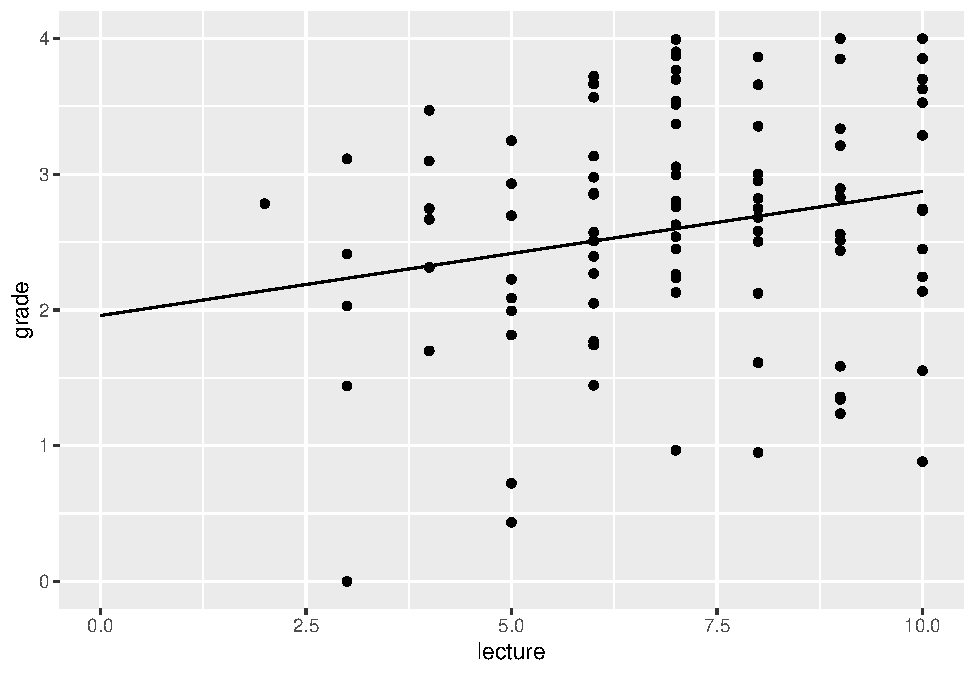
\includegraphics{03-多元回归_files/figure-latex/partial-lecture-plot-1.pdf}
\caption{\label{fig:partial-lecture-plot}nclicks固定在均值,\texttt{lecture}对成绩的偏效应}
\end{figure}

偏效应图只有在模型中焦点预测变量与其他预测变量之间没有交互效应时才有意义。

原因是当存在交互效应时,焦点预测变量\(X_i\)的偏效应会随着与其交互的变量的变动而变动。

现在你能可视化\texttt{nclicks}对\texttt{grade}的偏效应吗?

本页最后给出解决方法。

\hypertarget{ux6807ux51c6ux5316ux7cfbux6570}{%
\subsection{标准化系数}\label{ux6807ux51c6ux5316ux7cfbux6570}}

我们经常用多元回归来解决的一类问题是,\textbf{哪个预测变量对预测Y最重要?}

现在,你不能简单地读取\(\hat{\beta}\)值并选择绝对值最大的一个,因为这些预测变量都在不同的尺度上。为了回答这个问题,你需要对预测变量进行\textbf{中心化(center)}和\textbf{比例化(scale)}。

还记得\(z\)分数吗?

\[
z = \frac{X - \mu_x}{\sigma_x}
\]

\(z\)分数(\(z\)-score)表示\(X\)与样本均值(\(\mu_x\))之间的标准差单位距离(\(\sigma_x\))。因此,\(z\)分数为1意味着该值高于均值1个标准差;\(z\)分数为-2.5意味着低于均值2.5个标准差。\(Z\)分数通过将它们校准为标准正态分布(均值为0,标准差为1的分布)给了我们一种比较来自不同总体的事物的办法。

那么我们通过将预测变量转换为\(z\)分数来重新缩放它们。这是相当容易做到的。

\begin{Shaded}
\begin{Highlighting}[]
\NormalTok{grades2 }\OtherTok{\textless{}{-}}\NormalTok{ grades }\SpecialCharTok{\%\textgreater{}\%}
  \FunctionTok{mutate}\NormalTok{(}\AttributeTok{lecture\_c =}\NormalTok{ (lecture }\SpecialCharTok{{-}} \FunctionTok{mean}\NormalTok{(lecture)) }\SpecialCharTok{/} \FunctionTok{sd}\NormalTok{(lecture),}
         \AttributeTok{nclicks\_c =}\NormalTok{ (nclicks }\SpecialCharTok{{-}} \FunctionTok{mean}\NormalTok{(nclicks)) }\SpecialCharTok{/} \FunctionTok{sd}\NormalTok{(nclicks))}

\NormalTok{grades2}
\end{Highlighting}
\end{Shaded}

\begin{verbatim}
## # A tibble: 100 x 6
##    grade   GPA lecture nclicks lecture_c nclicks_c
##    <dbl> <dbl>   <int>   <int>     <dbl>     <dbl>
##  1  2.40 1.13        6      88  -0.484     -0.666 
##  2  3.67 0.971       6      96  -0.484     -0.150 
##  3  2.85 3.34        6     123  -0.484      1.59  
##  4  1.36 2.76        9      99   0.982      0.0439
##  5  2.31 1.02        4      66  -1.46      -2.09  
##  6  2.58 0.841       8      99   0.493      0.0439
##  7  2.69 4           5      86  -0.972     -0.796 
##  8  3.05 2.29        7     118   0.00488    1.27  
##  9  3.21 3.39        9      98   0.982     -0.0207
## 10  2.24 3.27       10     115   1.47       1.08  
## # i 90 more rows
\end{verbatim}

现在让我们用居中和缩放后的预测变量重新拟合模型。

\begin{Shaded}
\begin{Highlighting}[]
\NormalTok{my\_model\_scaled }\OtherTok{\textless{}{-}} \FunctionTok{lm}\NormalTok{(grade }\SpecialCharTok{\textasciitilde{}}\NormalTok{ lecture\_c }\SpecialCharTok{+}\NormalTok{ nclicks\_c, grades2)}

\FunctionTok{summary}\NormalTok{(my\_model\_scaled)}
\end{Highlighting}
\end{Shaded}

\begin{verbatim}
## 
## Call:
## lm(formula = grade ~ lecture_c + nclicks_c, data = grades2)
## 
## Residuals:
##      Min       1Q   Median       3Q      Max 
## -2.21653 -0.40603  0.02267  0.60720  1.38558 
## 
## Coefficients:
##             Estimate Std. Error t value Pr(>|t|)    
## (Intercept)  2.59839    0.08692  29.895   <2e-16 ***
## lecture_c    0.18734    0.09370   1.999   0.0484 *  
## nclicks_c    0.07823    0.09370   0.835   0.4058    
## ---
## Signif. codes:  0 '***' 0.001 '**' 0.01 '*' 0.05 '.' 0.1 ' ' 1
## 
## Residual standard error: 0.8692 on 97 degrees of freedom
## Multiple R-squared:  0.06543,    Adjusted R-squared:  0.04616 
## F-statistic: 3.395 on 2 and 97 DF,  p-value: 0.03756
\end{verbatim}

这告诉我们lecture\_c的影响相对更大,该变量每个标准差的提高,\texttt{grade}相应地提高0.19。

另一种常见的标准化方法是同时对响应变量和预测变量进行标准化,即对\(Y\)值和\(X\)值都进行\(z\)分数转换。采用这种方法时,回归系数的相对(影响力)排序将保持不变。主要区别在于,系数将反映响应变量以标准差(\(SD\))为单位的变化,而不是原始单位。

\textbf{多重共线性(multicollinearity)及其不足}

在关于多元回归的讨论中,你可能会听到对''多重共线性''的担忧,这是指预测变量之间存在交互关系的一种高级说法。这只是一个潜在的问题,因为它可能会影响对单个预测变量效应的解释。当预测变量相关时,\(\beta\)值可能会根据模型中包含或排除的预测变量而变化,有时甚至会改变符号。关于这一点需要记住的关键是:

\begin{itemize}
\tightlist
\item
  观察性研究(observational studies)中预测变量之间相关是不可避免的;
\item
  回归\textbf{不}假设你的预测变量彼此独立(换句话说,在预测变量之间找到相关性本身并不是质疑模型的理由);
\item
  当存在强相关时,解释单个回归系数时要谨慎;
\item
  目前没有已知的''补救措施'',也不清楚是否需要任何此类补救措施,许多所谓的补救措施弊大于利。
\end{itemize}

更多信息和指导请查阅 \citet{Vanhove_2021} 。

\hypertarget{ux6a21ux578bux6bd4ux8f83}{%
\subsection{模型比较}\label{ux6a21ux578bux6bd4ux8f83}}

另一种使用多元回归模型解决的常见问题是:某个预测变量或一组预测变量\textbf{在超出某些控制变量的影响之外},对我的响应变量有显著影响吗?

举个例子,上述包含\texttt{lecture}和\texttt{nclicks}的模型在统计上是显著的, \(F(2,97) = 3.395, p =0.038\)。

\(m\)个预测因子的回归模型的原假设(null hypothesis)为:

\[H_0: \beta_1 = \beta_2 = \ldots = \beta_m = 0;\]

换句话说,所有的系数(除了截距)都是0。如果原假设成立,那么原模型(null model)

\[Y_i = \beta_0\]

与包含所有预测变量及其系数的模型一样能给出很好的预测。换句话说,你对\(Y\)的最佳预测只是它的均值(\(\mu_y\));\(X\)变量是无关紧要的。我们拒绝了这个原假设,意味着通过纳入我们的两个预测变量\texttt{lecture}和\texttt{nclicks},可以做得更好。

但你可能会问:也许是成绩更好的学生获得了更好的成绩,而\texttt{lecture}、\texttt{nclicks}和\texttt{grade}之间的关系仅仅是通过学生质量的中介来实现。毕竟,成绩更好的学生更有可能去听讲座并下载材料。因此,我们可以问,出勤率和下载次数是否在\textbf{超出}学生能力(通过GPA测量)之外与更好的成绩相关?

我们可以通过\textbf{模型比较}来检验这一假设。逻辑是这样的:首先,估计一个包含所有控制预测变量但不包含焦点预测变量的模型。其次,估计一个包含控制预测变量和焦点预测变量的模型。最后,比较这两个模型,看看包含预测因子是否有统计学上显著的增益。

下面展示你如何做到这一点:

\begin{Shaded}
\begin{Highlighting}[]
\NormalTok{m1 }\OtherTok{\textless{}{-}} \FunctionTok{lm}\NormalTok{(grade }\SpecialCharTok{\textasciitilde{}}\NormalTok{ GPA, grades) }\CommentTok{\# control model}
\NormalTok{m2 }\OtherTok{\textless{}{-}} \FunctionTok{lm}\NormalTok{(grade }\SpecialCharTok{\textasciitilde{}}\NormalTok{ GPA }\SpecialCharTok{+}\NormalTok{ lecture }\SpecialCharTok{+}\NormalTok{ nclicks, grades) }\CommentTok{\# bigger model}

\FunctionTok{anova}\NormalTok{(m1, m2)}
\end{Highlighting}
\end{Shaded}

\begin{verbatim}
## Analysis of Variance Table
## 
## Model 1: grade ~ GPA
## Model 2: grade ~ GPA + lecture + nclicks
##   Res.Df    RSS Df Sum of Sq      F Pr(>F)
## 1     98 73.528                           
## 2     96 71.578  2    1.9499 1.3076 0.2752
\end{verbatim}

原假设是我们仅通过\texttt{GPA}预测\texttt{grade}与通过\texttt{GPA}加上\texttt{lecture}和\texttt{nclicks}预测\texttt{grade}一样准确。如果添加这两个变量能够显著减少\textbf{残差平方和(RSS)},即它们能解释足够多的残差方差,我们就会拒绝这个原假设。

我们看到情况并非如此:\(F(2,96) = 1.308\), \(p =0.275\)。因此,我们没有证据表明课堂出勤率和下载在线材料在通过GPA衡量的学生能力之外与更好的成绩相关。

\hypertarget{ux5904ux7406ux5206ux7c7bux9884ux6d4bux53d8ux91cf}{%
\section{处理分类预测变量}\label{ux5904ux7406ux5206ux7c7bux9884ux6d4bux53d8ux91cf}}

回归公式将响应变量描述为加权预测变量的总和。但如果其中一个预测变量是分类变量(如代表''农村''或''城市''等群组),而不是数值型变量会怎样呢?许多变量是\textbf{名义(nominal)}变量:包含名称的分类变量,在变量的级别之间没有固有的顺序。例如,宠物所有权(猫、狗、雪貂)是一个名义变量;不考虑喜好,拥有猫不等于拥有狗,拥有狗不等于拥有雪貂。

\textbf{使用数值型预测变量表示名义数据}

在回归模型中表示一个\(k\)水平的名义变量需要\(k-1\)个数值型预测变量;例如,如果有4水平,你需要3个预测变量。大多数编码方案要求你在\(k\)个水平中选择一个作为基线水平。\(k-1\)个变量中,每个变量都是其表示的水平与基线水平对比。

\textbf{举例:}你有一个三水平变量\texttt{pet\_type}(猫、狗、雪貂)。

你选择猫为基线并创建两个数值型预测变量:

\begin{itemize}
\tightlist
\item
  \texttt{dog\_v\_cat}用来编码狗和猫之间的对比;
\item
  \texttt{ferret\_v\_cat}用来编码雪貂和猫之间的对比。
\end{itemize}

名义变量通常在数据框中表示\texttt{character}或\texttt{factor}类型。

字符(character)变量和因子(factor)变量的区别在于因子包含关于水平及其顺序的信息,而字符向量则缺乏此信息。

当你使用R公式语法(R formula syntax)指定模型时,R会检查公式右侧预测变量的数据类型。例如,如果你的模型将\texttt{income}回归到\texttt{pet\_type}上(\texttt{income\ \textasciitilde{}\ pet\_type}),R会检查\texttt{pet\_type}的数据类型。

对于所有类型为字符或因子的变量,R都会隐式地(implicitly)创建一个(或一组)数值型预测变量来表示该变量在模型中的作用。有多种方案可用于创建名义变量的数值表示。R中的默认方法是使用\textbf{虚拟}(dummy,或叫处理(treatment))编码(见下文)。不幸的是,这种默认方法(注:不是指虚拟编码,而是指R自动建立虚拟编码)不适合心理学中的许多研究设计,因此我建议你学习如何``手动''编码你的预测变量,并养成这样做的习惯。

\textbf{不要用数字表示分类变量的水平!}

上述例子中,我们有一个名为\texttt{pet\_type}的变量,其水平为\texttt{cat}、\texttt{dog}和\texttt{ferret}。有时人们用数字表示名义变量的水平,像这样:

\begin{itemize}
\tightlist
\item
  \texttt{1}表示猫,
\item
  \texttt{2}表示狗,
\item
  \texttt{3}表示雪貂。
\end{itemize}

这是个坏主意。

首先,这样的标记是任意且不透明的,任何试图使用你数据的人都不知道哪个数字对应哪个类别(你自己也可能会忘记!)。

更糟糕的是,如果你把这个变量作为回归模型中的预测变量引入,R将无法知道你使用1、2和3作为变量内各水平标签的意图,而是会假设\texttt{pet\_type}是一个测量值,其中狗比猫大1个单位,雪貂比猫大2个单位,比狗大1个单位,这完全是无意义的!

这种错误太容易犯了,而且如果作者不分享他们的数据和代码,这很难发现。2016年,\href{https://www.sciencedirect.com/science/article/pii/S0960982216306704}{《Current Biology》发表的一篇关于儿童宗教信仰和利他行为的论文就因为这种错误而被撤稿}。

所以,不要用数字来表示名义变量的各个水平,除非你是有意创建预测变量来编码代表名义变量的\(k-1\)对比项,以便在回归模型中正确表示名义变量。

\hypertarget{ux865aux62dfux7f16ux7801ux53c8ux79f0ux5904ux7406ux7f16ux7801}{%
\subsection{虚拟编码(又称``处理''编码)}\label{ux865aux62dfux7f16ux7801ux53c8ux79f0ux5904ux7406ux7f16ux7801}}

对于只有两个水平的名义变量,选择一个水平作为基线,并创建一个新变量,当名义变量是基线时,该新变量为\texttt{0},非基线时为\texttt{1}。基线的选择是任意的,只会影响系数是正还是负,但不会影响大小、标准误或相关的p值。

为了说明这点,让我们生成一些只包含一个两水平分类预测变量的假数据。

\begin{Shaded}
\begin{Highlighting}[]
\NormalTok{fake\_data }\OtherTok{\textless{}{-}} \FunctionTok{tibble}\NormalTok{(}\AttributeTok{Y =} \FunctionTok{rnorm}\NormalTok{(}\DecValTok{10}\NormalTok{),}
                    \AttributeTok{group =} \FunctionTok{rep}\NormalTok{(}\FunctionTok{c}\NormalTok{(}\StringTok{"A"}\NormalTok{, }\StringTok{"B"}\NormalTok{), }\AttributeTok{each =} \DecValTok{5}\NormalTok{))}

\NormalTok{fake\_data}
\end{Highlighting}
\end{Shaded}

\begin{verbatim}
## # A tibble: 10 x 2
##         Y group
##     <dbl> <chr>
##  1  2.01  A    
##  2  0.673 A    
##  3 -0.597 A    
##  4  0.141 A    
##  5 -0.649 A    
##  6  0.519 B    
##  7 -0.805 B    
##  8  1.85  B    
##  9  1.28  B    
## 10  1.47  B
\end{verbatim}

现在让我们来添加一个新变量\texttt{group\_d},这是经过虚拟编码的分组变量。我们将使用\texttt{dplyr::if\_else()}函数来定义新列。

\begin{Shaded}
\begin{Highlighting}[]
\NormalTok{fake\_data2 }\OtherTok{\textless{}{-}}\NormalTok{ fake\_data }\SpecialCharTok{\%\textgreater{}\%}
  \FunctionTok{mutate}\NormalTok{(}\AttributeTok{group\_d =} \FunctionTok{if\_else}\NormalTok{(group }\SpecialCharTok{==} \StringTok{"B"}\NormalTok{, }\DecValTok{1}\NormalTok{, }\DecValTok{0}\NormalTok{))}

\NormalTok{fake\_data2}
\end{Highlighting}
\end{Shaded}

\begin{verbatim}
## # A tibble: 10 x 3
##         Y group group_d
##     <dbl> <chr>   <dbl>
##  1  2.01  A           0
##  2  0.673 A           0
##  3 -0.597 A           0
##  4  0.141 A           0
##  5 -0.649 A           0
##  6  0.519 B           1
##  7 -0.805 B           1
##  8  1.85  B           1
##  9  1.28  B           1
## 10  1.47  B           1
\end{verbatim}

现在我们把它作为常规的回归模型来运行。

\begin{Shaded}
\begin{Highlighting}[]
\FunctionTok{summary}\NormalTok{(}\FunctionTok{lm}\NormalTok{(Y }\SpecialCharTok{\textasciitilde{}}\NormalTok{ group\_d, fake\_data2))}
\end{Highlighting}
\end{Shaded}

\begin{verbatim}
## 
## Call:
## lm(formula = Y ~ group_d, data = fake_data2)
## 
## Residuals:
##     Min      1Q  Median      3Q     Max 
## -1.6662 -0.7705  0.0906  0.5578  1.6979 
## 
## Coefficients:
##             Estimate Std. Error t value Pr(>|t|)
## (Intercept)   0.3164     0.4800   0.659    0.528
## group_d       0.5449     0.6789   0.803    0.445
## 
## Residual standard error: 1.073 on 8 degrees of freedom
## Multiple R-squared:  0.07455,    Adjusted R-squared:  -0.04114 
## F-statistic: 0.6444 on 1 and 8 DF,  p-value: 0.4453
\end{verbatim}

让我们反转编码。我们得到相同的结果,只是符号不同。

\begin{Shaded}
\begin{Highlighting}[]
\NormalTok{fake\_data3 }\OtherTok{\textless{}{-}}\NormalTok{ fake\_data }\SpecialCharTok{\%\textgreater{}\%}
  \FunctionTok{mutate}\NormalTok{(}\AttributeTok{group\_d =} \FunctionTok{if\_else}\NormalTok{(group }\SpecialCharTok{==} \StringTok{"A"}\NormalTok{, }\DecValTok{1}\NormalTok{, }\DecValTok{0}\NormalTok{))}

\FunctionTok{summary}\NormalTok{(}\FunctionTok{lm}\NormalTok{(Y }\SpecialCharTok{\textasciitilde{}}\NormalTok{ group\_d, fake\_data3))}
\end{Highlighting}
\end{Shaded}

\begin{verbatim}
## 
## Call:
## lm(formula = Y ~ group_d, data = fake_data3)
## 
## Residuals:
##     Min      1Q  Median      3Q     Max 
## -1.6662 -0.7705  0.0906  0.5578  1.6979 
## 
## Coefficients:
##             Estimate Std. Error t value Pr(>|t|)
## (Intercept)   0.8614     0.4800   1.794    0.110
## group_d      -0.5449     0.6789  -0.803    0.445
## 
## Residual standard error: 1.073 on 8 degrees of freedom
## Multiple R-squared:  0.07455,    Adjusted R-squared:  -0.04114 
## F-statistic: 0.6444 on 1 and 8 DF,  p-value: 0.4453
\end{verbatim}

截距的解释是编码为0的组的估计均值。你可以通过将0代入到下面的预测公式中的X看到这一点。因此,\(\beta_1\)可以解释为基线组和编码为1的组之间的均值差异。

\[\hat{Y_i} = \hat{\beta}_0 + \hat{\beta}_1 X_i \]

请注意,如果我们只是将字符变量\texttt{group}作为模型的预测变量,R将根据需要自动为我们创建虚拟变量。

\begin{Shaded}
\begin{Highlighting}[]
\FunctionTok{lm}\NormalTok{(Y }\SpecialCharTok{\textasciitilde{}}\NormalTok{ group, fake\_data) }\SpecialCharTok{\%\textgreater{}\%}
  \FunctionTok{summary}\NormalTok{()}
\end{Highlighting}
\end{Shaded}

\begin{verbatim}
## 
## Call:
## lm(formula = Y ~ group, data = fake_data)
## 
## Residuals:
##     Min      1Q  Median      3Q     Max 
## -1.6662 -0.7705  0.0906  0.5578  1.6979 
## 
## Coefficients:
##             Estimate Std. Error t value Pr(>|t|)
## (Intercept)   0.3164     0.4800   0.659    0.528
## groupB        0.5449     0.6789   0.803    0.445
## 
## Residual standard error: 1.073 on 8 degrees of freedom
## Multiple R-squared:  0.07455,    Adjusted R-squared:  -0.04114 
## F-statistic: 0.6444 on 1 and 8 DF,  p-value: 0.4453
\end{verbatim}

\texttt{lm()}函数检查\texttt{group}并确定变量不同的水平------在这种情况下是\texttt{A}和\texttt{B}。然后,它选择按字母顺序排在最前面的水平作为基线(注:中文一样是字母顺序),并编码另一个水平(\texttt{B})与基线水平(\texttt{A})之间的对比。(如果\texttt{group}被定义为因子,基线水平就是\texttt{levels(fake\_data\$group)}的第一个元素)。

它创建的新变量以\texttt{groupB}的名称出现在输出中。

\hypertarget{ux5f53k-2ux65f6ux7684ux865aux62dfux7f16ux7801}{%
\subsection{\texorpdfstring{当\(k > 2\)时的虚拟编码}{当k \textgreater{} 2时的虚拟编码}}\label{ux5f53k-2ux65f6ux7684ux865aux62dfux7f16ux7801}}

当名义预测变量超过两水平(\(k > 2\))时,一个数值预测变量就不够用了,我们需要\(k-1\)个预测变量。如果名义预测变量有4水平,我们将需要定义3个预测变量。让我们模拟一些要处理的数据,\texttt{season\_wt}表示一年四季一个人的体重(以kg为单位)。

\begin{Shaded}
\begin{Highlighting}[]
\NormalTok{season\_wt }\OtherTok{\textless{}{-}} \FunctionTok{tibble}\NormalTok{(}\AttributeTok{season =} \FunctionTok{rep}\NormalTok{(}\FunctionTok{c}\NormalTok{(}\StringTok{"winter"}\NormalTok{, }\StringTok{"spring"}\NormalTok{, }\StringTok{"summer"}\NormalTok{, }\StringTok{"fall"}\NormalTok{),}
                                 \AttributeTok{each =} \DecValTok{5}\NormalTok{),}
                    \AttributeTok{bodyweight\_kg =} \FunctionTok{c}\NormalTok{(}\FunctionTok{rnorm}\NormalTok{(}\DecValTok{5}\NormalTok{, }\DecValTok{105}\NormalTok{, }\DecValTok{3}\NormalTok{),}
                                      \FunctionTok{rnorm}\NormalTok{(}\DecValTok{5}\NormalTok{, }\DecValTok{103}\NormalTok{, }\DecValTok{3}\NormalTok{),}
                                      \FunctionTok{rnorm}\NormalTok{(}\DecValTok{5}\NormalTok{, }\DecValTok{101}\NormalTok{, }\DecValTok{3}\NormalTok{),}
                                      \FunctionTok{rnorm}\NormalTok{(}\DecValTok{5}\NormalTok{, }\FloatTok{102.5}\NormalTok{, }\DecValTok{3}\NormalTok{)))}

\NormalTok{season\_wt}
\end{Highlighting}
\end{Shaded}

\begin{verbatim}
## # A tibble: 20 x 2
##    season bodyweight_kg
##    <chr>          <dbl>
##  1 winter         103. 
##  2 winter         106. 
##  3 winter         108. 
##  4 winter         105. 
##  5 winter         104. 
##  6 spring         106. 
##  7 spring         105. 
##  8 spring          96.8
##  9 spring         106. 
## 10 spring         104. 
## 11 summer          99.5
## 12 summer         101. 
## 13 summer         105. 
## 14 summer         100. 
## 15 summer         103. 
## 16 fall           105. 
## 17 fall           102. 
## 18 fall            97.7
## 19 fall           105. 
## 20 fall            96.1
\end{verbatim}

现在让我们添加三个预测变量来编码变量\texttt{season}。尝试一下,看看你是否能弄清楚了它是如何工作的。

\begin{Shaded}
\begin{Highlighting}[]
\DocumentationTok{\#\# 基线变量是“winter”}
\NormalTok{season\_wt2 }\OtherTok{\textless{}{-}}\NormalTok{ season\_wt }\SpecialCharTok{\%\textgreater{}\%}
  \FunctionTok{mutate}\NormalTok{(}\AttributeTok{spring\_v\_winter =} \FunctionTok{if\_else}\NormalTok{(season }\SpecialCharTok{==} \StringTok{"spring"}\NormalTok{, }\DecValTok{1}\NormalTok{, }\DecValTok{0}\NormalTok{),}
         \AttributeTok{summer\_v\_winter =} \FunctionTok{if\_else}\NormalTok{(season }\SpecialCharTok{==} \StringTok{"summer"}\NormalTok{, }\DecValTok{1}\NormalTok{, }\DecValTok{0}\NormalTok{),}
         \AttributeTok{fall\_v\_winter =} \FunctionTok{if\_else}\NormalTok{(season }\SpecialCharTok{==} \StringTok{"fall"}\NormalTok{, }\DecValTok{1}\NormalTok{, }\DecValTok{0}\NormalTok{))}

\NormalTok{season\_wt2}
\end{Highlighting}
\end{Shaded}

\begin{verbatim}
## # A tibble: 20 x 5
##    season bodyweight_kg spring_v_winter summer_v_winter fall_v_winter
##    <chr>          <dbl>           <dbl>           <dbl>         <dbl>
##  1 winter         103.                0               0             0
##  2 winter         106.                0               0             0
##  3 winter         108.                0               0             0
##  4 winter         105.                0               0             0
##  5 winter         104.                0               0             0
##  6 spring         106.                1               0             0
##  7 spring         105.                1               0             0
##  8 spring          96.8               1               0             0
##  9 spring         106.                1               0             0
## 10 spring         104.                1               0             0
## 11 summer          99.5               0               1             0
## 12 summer         101.                0               1             0
## 13 summer         105.                0               1             0
## 14 summer         100.                0               1             0
## 15 summer         103.                0               1             0
## 16 fall           105.                0               0             1
## 17 fall           102.                0               0             1
## 18 fall            97.7               0               0             1
## 19 fall           105.                0               0             1
## 20 fall            96.1               0               0             1
\end{verbatim}

\textbf{提醒:始终查看你的数据}

每当你写的代码可能改变数据时,都应该通过查看数据来确保代码按预期工作。这在你手动编码用于回归的名义变量时尤其重要,因为有时代码会写错,但不会引发报错。

考虑上面的代码块,我们定义了三个对比来表示名义变量\texttt{season},\texttt{winter}是我们的基线。

如果你意外地拼错了一个水平(使用\texttt{summre}而不是\texttt{summer}),你能注意到吗?

\begin{Shaded}
\begin{Highlighting}[]
\NormalTok{season\_wt3 }\OtherTok{\textless{}{-}}\NormalTok{ season\_wt }\SpecialCharTok{\%\textgreater{}\%}
  \FunctionTok{mutate}\NormalTok{(}\AttributeTok{spring\_v\_winter =} \FunctionTok{if\_else}\NormalTok{(season }\SpecialCharTok{==} \StringTok{"spring"}\NormalTok{, }\DecValTok{1}\NormalTok{, }\DecValTok{0}\NormalTok{),}
         \AttributeTok{summer\_v\_winter =} \FunctionTok{if\_else}\NormalTok{(season }\SpecialCharTok{==} \StringTok{"summre"}\NormalTok{, }\DecValTok{1}\NormalTok{, }\DecValTok{0}\NormalTok{),}
         \AttributeTok{fall\_v\_winter =} \FunctionTok{if\_else}\NormalTok{(season }\SpecialCharTok{==} \StringTok{"fall"}\NormalTok{, }\DecValTok{1}\NormalTok{, }\DecValTok{0}\NormalTok{))}
\end{Highlighting}
\end{Shaded}

虽然上面的代码块可以运行,但当我们运行回归时,我们会得到令人困惑的输出,即\texttt{summer\_v\_winter}的系数是\texttt{NA}(不可用,not available)。

\begin{Shaded}
\begin{Highlighting}[]
\FunctionTok{lm}\NormalTok{(bodyweight\_kg }\SpecialCharTok{\textasciitilde{}}\NormalTok{ spring\_v\_winter }\SpecialCharTok{+}\NormalTok{ summer\_v\_winter }\SpecialCharTok{+}\NormalTok{ fall\_v\_winter,}
\NormalTok{   season\_wt3)}
\end{Highlighting}
\end{Shaded}

\begin{verbatim}
## 
## Call:
## lm(formula = bodyweight_kg ~ spring_v_winter + summer_v_winter + 
##     fall_v_winter, data = season_wt3)
## 
## Coefficients:
##     (Intercept)  spring_v_winter  summer_v_winter    fall_v_winter  
##        103.4048           0.2287               NA          -2.4060
\end{verbatim}

发生了什么?让我们看看数据来找到答案。我们将使用\texttt{distinct}函数找出原始变量\texttt{season}和我们创建的三个变量的不同组合(详细信息参见\texttt{?dplyr::distinct})。

\begin{Shaded}
\begin{Highlighting}[]
\NormalTok{season\_wt3 }\SpecialCharTok{\%\textgreater{}\%}
  \FunctionTok{distinct}\NormalTok{(season, spring\_v\_winter, summer\_v\_winter, fall\_v\_winter)}
\end{Highlighting}
\end{Shaded}

\begin{verbatim}
## # A tibble: 4 x 4
##   season spring_v_winter summer_v_winter fall_v_winter
##   <chr>            <dbl>           <dbl>         <dbl>
## 1 winter               0               0             0
## 2 spring               1               0             0
## 3 summer               0               0             0
## 4 fall                 0               0             1
\end{verbatim}

由于我们的拼写错误,当\texttt{season\ ==\ "summer"}时,预测变量\texttt{summer\_v\_winter}不是\texttt{1};相反,它\textbf{总是0}。\texttt{if\_else()}字面上意思是``如果\texttt{season\ ==\ "summre"},则将\texttt{summer\_v\_winter}设置为1,否则为0''。当然,\texttt{season}\textbf{永远}不会等于\texttt{summre},因为\texttt{summre}是一个拼写错误。我们本可以通过使用\texttt{distinct()}进行上面的检查轻松发现这一点。当你创建自己的数值预测变量时,养成这样做的习惯是很重要的。

\textbf{更仔细地看看R的默认情况}

如果你曾经使用过像SPSS这样的指向-点击的统计软件,你可能从未学习过如何编码分类预测变量。通常,软件会识别预测变量是否为分类变量,并在后台将其重新编码为数值型预测变量。R也是如此:如果你将\texttt{character}或\texttt{factor}类型的预测变量提供给线性建模函数,它将为你创建数值型虚拟编码的预测变量,如下方代码所示。

\begin{Shaded}
\begin{Highlighting}[]
\FunctionTok{lm}\NormalTok{(bodyweight\_kg }\SpecialCharTok{\textasciitilde{}}\NormalTok{ season, season\_wt) }\SpecialCharTok{\%\textgreater{}\%}
  \FunctionTok{summary}\NormalTok{()}
\end{Highlighting}
\end{Shaded}

\begin{verbatim}
## 
## Call:
## lm(formula = bodyweight_kg ~ season, data = season_wt)
## 
## Residuals:
##     Min      1Q  Median      3Q     Max 
## -6.7880 -1.6166  0.4861  2.5731  3.6763 
## 
## Coefficients:
##              Estimate Std. Error t value Pr(>|t|)    
## (Intercept)  100.9988     1.4102  71.620   <2e-16 ***
## seasonspring   2.6347     1.9943   1.321   0.2051    
## seasonsummer   0.8371     1.9943   0.420   0.6802    
## seasonwinter   3.9748     1.9943   1.993   0.0636 .  
## ---
## Signif. codes:  0 '***' 0.001 '**' 0.01 '*' 0.05 '.' 0.1 ' ' 1
## 
## Residual standard error: 3.153 on 16 degrees of freedom
## Multiple R-squared:  0.2314, Adjusted R-squared:  0.08726 
## F-statistic: 1.605 on 3 and 16 DF,  p-value: 0.2274
\end{verbatim}

在这里,R隐式地创建了三个虚拟变量来编码\texttt{season}的四个水平,分别命名为\texttt{seasonspring}、\texttt{seasonsummer}和\texttt{seasonwinter}。未提及的季节\texttt{fall}被选为基线,因为它在字母表中最早出现。这三个预测变量的值如下:

\begin{itemize}
\tightlist
\item
  \texttt{seasonspring}:如果是春季则为\texttt{1},否则为\texttt{0};
\item
  \texttt{seasonsummer}:如果是夏季则为\texttt{1},否则为\texttt{0};
\item
  \texttt{seasonwinter}:如果是冬季则为\texttt{1},否则为\texttt{0};
\end{itemize}

这似乎是让R为我们做的一件方便的事情,但是在按赖默认设置时可能会有潜在风险。在下一章中,当我们讨论交互效应时,我们将更多地了解这些风险。

\hypertarget{ux591aux5143ux56deux5f52ux548cux5355ux56e0ux7d20ux65b9ux5deeux5206ux6790one-way-anovaux7684ux7b49ux4ef7ux6027}{%
\section{多元回归和单因素方差分析(one-way ANOVA)的等价性}\label{ux591aux5143ux56deux5f52ux548cux5355ux56e0ux7d20ux65b9ux5deeux5206ux6790one-way-anovaux7684ux7b49ux4ef7ux6027}}

如果我们想要查看我们的体重是否随季节变化,我们可以对\texttt{season\_wt2}进行单因素方差分析,如下所示。

\begin{Shaded}
\begin{Highlighting}[]
\DocumentationTok{\#\# 将季节变为一个以“winter”为基线的因子变量}
\NormalTok{season\_wt3 }\OtherTok{\textless{}{-}}\NormalTok{ season\_wt2 }\SpecialCharTok{\%\textgreater{}\%}
  \FunctionTok{mutate}\NormalTok{(}\AttributeTok{season =} \FunctionTok{factor}\NormalTok{(season, }\AttributeTok{levels =} \FunctionTok{c}\NormalTok{(}\StringTok{"winter"}\NormalTok{, }\StringTok{"spring"}\NormalTok{,}
                                            \StringTok{"summer"}\NormalTok{, }\StringTok{"fall"}\NormalTok{)))}

\NormalTok{my\_anova }\OtherTok{\textless{}{-}} \FunctionTok{aov}\NormalTok{(bodyweight\_kg }\SpecialCharTok{\textasciitilde{}}\NormalTok{ season, season\_wt3)}
\FunctionTok{summary}\NormalTok{(my\_anova)}
\end{Highlighting}
\end{Shaded}

\begin{verbatim}
##             Df Sum Sq Mean Sq F value Pr(>F)
## season       3  47.89  15.964   1.605  0.227
## Residuals   16 159.09   9.943
\end{verbatim}

好了,现在我们可以用下面的回归模型复制这个结果吗?

\[Y_i = \beta_0 + \beta_1 X_{1i} + \beta_2 X_{2i} + \beta_3 X_{3i} + e_i\]

\begin{Shaded}
\begin{Highlighting}[]
\FunctionTok{summary}\NormalTok{(}\FunctionTok{lm}\NormalTok{(bodyweight\_kg }\SpecialCharTok{\textasciitilde{}}\NormalTok{ spring\_v\_winter }\SpecialCharTok{+}
\NormalTok{             summer\_v\_winter }\SpecialCharTok{+}\NormalTok{ fall\_v\_winter,}
\NormalTok{           season\_wt2))}
\end{Highlighting}
\end{Shaded}

\begin{verbatim}
## 
## Call:
## lm(formula = bodyweight_kg ~ spring_v_winter + summer_v_winter + 
##     fall_v_winter, data = season_wt2)
## 
## Residuals:
##     Min      1Q  Median      3Q     Max 
## -6.7880 -1.6166  0.4861  2.5731  3.6763 
## 
## Coefficients:
##                 Estimate Std. Error t value Pr(>|t|)    
## (Intercept)      104.974      1.410  74.439   <2e-16 ***
## spring_v_winter   -1.340      1.994  -0.672   0.5112    
## summer_v_winter   -3.138      1.994  -1.573   0.1352    
## fall_v_winter     -3.975      1.994  -1.993   0.0636 .  
## ---
## Signif. codes:  0 '***' 0.001 '**' 0.01 '*' 0.05 '.' 0.1 ' ' 1
## 
## Residual standard error: 3.153 on 16 degrees of freedom
## Multiple R-squared:  0.2314, Adjusted R-squared:  0.08726 
## F-statistic: 1.605 on 3 and 16 DF,  p-value: 0.2274
\end{verbatim}

请注意,这两种方法的 \(F\) 值和 \(p\) 值是相同的!

\hypertarget{ux7ec3ux4e60ux7b54ux6848}{%
\section{练习答案}\label{ux7ec3ux4e60ux7b54ux6848}}

展开答案

首先创建一个包含新预测变量的tibble。我们可能还想知道\texttt{nclicks}的取值范围。

\begin{Shaded}
\begin{Highlighting}[]
\NormalTok{lecture\_mean }\OtherTok{\textless{}{-}}\NormalTok{ grades }\SpecialCharTok{\%\textgreater{}\%} \FunctionTok{pull}\NormalTok{(lecture) }\SpecialCharTok{\%\textgreater{}\%} \FunctionTok{mean}\NormalTok{()}
\NormalTok{min\_nclicks }\OtherTok{\textless{}{-}}\NormalTok{ grades }\SpecialCharTok{\%\textgreater{}\%} \FunctionTok{pull}\NormalTok{(nclicks) }\SpecialCharTok{\%\textgreater{}\%} \FunctionTok{min}\NormalTok{()}
\NormalTok{max\_nclicks }\OtherTok{\textless{}{-}}\NormalTok{ grades }\SpecialCharTok{\%\textgreater{}\%} \FunctionTok{pull}\NormalTok{(nclicks) }\SpecialCharTok{\%\textgreater{}\%} \FunctionTok{max}\NormalTok{()}

\DocumentationTok{\#\# 预测变量的新数据}
\NormalTok{new\_nclicks }\OtherTok{\textless{}{-}} \FunctionTok{tibble}\NormalTok{(}\AttributeTok{lecture =}\NormalTok{ lecture\_mean,}
                      \AttributeTok{nclicks =}\NormalTok{ min\_nclicks}\SpecialCharTok{:}\NormalTok{max\_nclicks)}

\DocumentationTok{\#\# 将预测值添加到new\_lecture中}
\NormalTok{new\_nclicks2 }\OtherTok{\textless{}{-}}\NormalTok{ new\_nclicks }\SpecialCharTok{\%\textgreater{}\%}
  \FunctionTok{mutate}\NormalTok{(}\AttributeTok{grade =} \FunctionTok{predict}\NormalTok{(my\_model, new\_nclicks))}

\NormalTok{new\_nclicks2}
\end{Highlighting}
\end{Shaded}

\begin{verbatim}
## # A tibble: 76 x 3
##    lecture nclicks grade
##      <dbl>   <int> <dbl>
##  1    6.99      54  2.37
##  2    6.99      55  2.38
##  3    6.99      56  2.38
##  4    6.99      57  2.39
##  5    6.99      58  2.39
##  6    6.99      59  2.40
##  7    6.99      60  2.40
##  8    6.99      61  2.41
##  9    6.99      62  2.41
## 10    6.99      63  2.42
## # i 66 more rows
\end{verbatim}

现在作图。

\begin{Shaded}
\begin{Highlighting}[]
\FunctionTok{ggplot}\NormalTok{(grades, }\FunctionTok{aes}\NormalTok{(nclicks, grade)) }\SpecialCharTok{+}
  \FunctionTok{geom\_point}\NormalTok{() }\SpecialCharTok{+}
  \FunctionTok{geom\_line}\NormalTok{(}\AttributeTok{data =}\NormalTok{ new\_nclicks2)}
\end{Highlighting}
\end{Shaded}

\begin{figure}
\centering
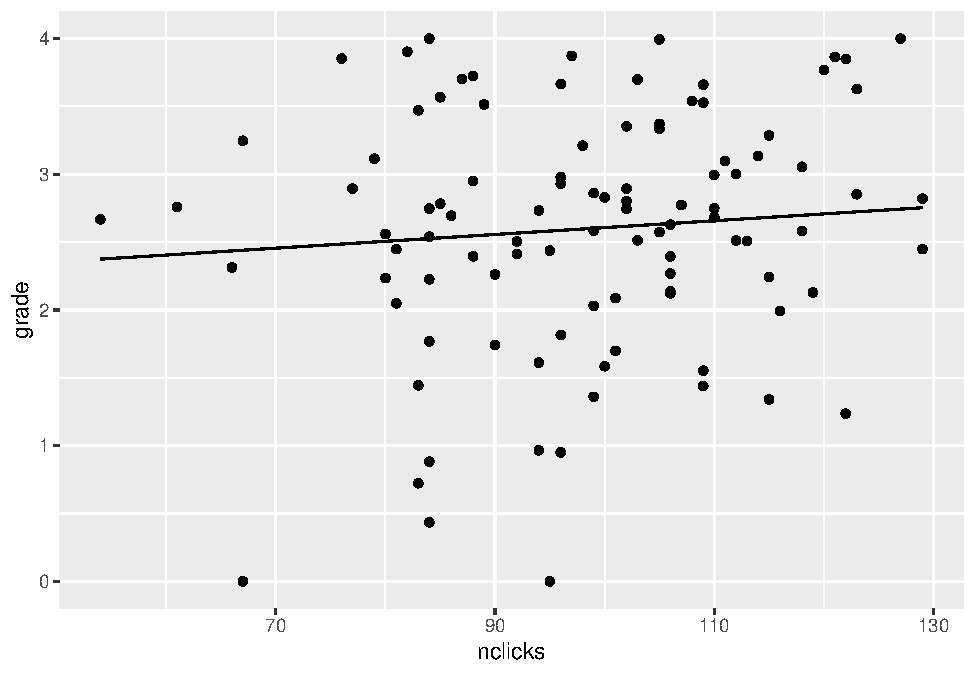
\includegraphics{03-多元回归_files/figure-latex/partial-nclicks-1.pdf}
\caption{\label{fig:partial-nclicks}nclicks对grade的偏效应图}
\end{figure}

\hypertarget{ux4ea4ux4e92ux6548ux5e94}{%
\chapter{交互效应}\label{ux4ea4ux4e92ux6548ux5e94}}

到目前为止,我们一直专注于估计和解释一个变量或预测变量线性组合对响应变量的影响。然而,往往存在这样的情况,一个预测变量对响应变量的影响取决于另一个预测变量。实际上,我们可以在模型中包含一个\textbf{交互}项来估计和解释这种依赖性。

\hypertarget{cont-by-cat}{%
\section{连续变量-分类变量交互效应}\label{cont-by-cat}}

让我们考虑一个简单的虚构例子。假设你对声波干扰对认知表现的影响感兴趣。你的研究中的每个被试在执行一个简单的反应时任务时(尽快对闪光灯做出反应),被随机分配接受特定水平的声波干扰。你有一种技术,可以自动生成不同水平的背景噪音(例如城市声音的频率和振幅:鸣笛声、钻地声、喧哗声、玻璃破碎声等)。每个参与者在一个随机选择的干扰水平(0到100)下执行任务。你的假设是,城市生活使人们的任务表现更不受声波干扰的影响。你想要比较城市居民和乡村居民(来自更安静的乡村环境)之间干扰与表现关系的差异。

你有3个变量:

\begin{itemize}
\tightlist
\item
  一个连续响应变量,\texttt{mean\_RT},其较高的水平反映较慢的反应时;
\item
  一个连续预测变量,声波干扰水平(\texttt{dist\_level}),其较高的水平表示更多的干扰;
\item
  一个两水平的因子,\texttt{group} (城市vs.乡村)。
\end{itemize}

让我们从模拟一些城市组的数据开始。假设在0干扰(静音)下,平均反应时约为450毫秒,且干扰每增加1个单位,反应时就增加约2毫秒。这给了我们以下线性模型:

\[Y_i = 450 + 2 X_i + e_i\]

其中\(X_i\)是声音干扰的水平。

让我们模拟100名被试的数据,设定\(\sigma = 80\),并在开始之前设置种子。

\begin{Shaded}
\begin{Highlighting}[]
\FunctionTok{library}\NormalTok{(tidyverse)}
\FunctionTok{set.seed}\NormalTok{(}\DecValTok{1031}\NormalTok{)}

\NormalTok{n\_subj }\OtherTok{\textless{}{-}}\NormalTok{ 100L  }\CommentTok{\# 模拟100名被试的数据(注:L是说明100是整数)}
\NormalTok{b0\_urban }\OtherTok{\textless{}{-}} \DecValTok{450} \CommentTok{\# y轴截距}
\NormalTok{b1\_urban }\OtherTok{\textless{}{-}} \DecValTok{2}   \CommentTok{\# 斜率}

\CommentTok{\# 分解表(decomposition table)}
\NormalTok{urban }\OtherTok{\textless{}{-}} \FunctionTok{tibble}\NormalTok{(}
  \AttributeTok{subj\_id =} \DecValTok{1}\SpecialCharTok{:}\NormalTok{n\_subj,}
  \AttributeTok{group =} \StringTok{"urban"}\NormalTok{,}
  \AttributeTok{b0 =} \DecValTok{450}\NormalTok{,}
  \AttributeTok{b1 =} \DecValTok{2}\NormalTok{,}
  \AttributeTok{dist\_level =} \FunctionTok{sample}\NormalTok{(}\DecValTok{0}\SpecialCharTok{:}\NormalTok{n\_subj, n\_subj, }\AttributeTok{replace =} \ConstantTok{TRUE}\NormalTok{),}
  \AttributeTok{err =} \FunctionTok{rnorm}\NormalTok{(n\_subj, }\AttributeTok{mean =} \DecValTok{0}\NormalTok{, }\AttributeTok{sd =} \DecValTok{80}\NormalTok{),}
  \AttributeTok{simple\_rt =}\NormalTok{ b0 }\SpecialCharTok{+}\NormalTok{ b1 }\SpecialCharTok{*}\NormalTok{ dist\_level }\SpecialCharTok{+}\NormalTok{ err)}

\NormalTok{urban}
\end{Highlighting}
\end{Shaded}

\begin{verbatim}
## # A tibble: 100 x 7
##    subj_id group    b0    b1 dist_level     err simple_rt
##      <int> <chr> <dbl> <dbl>      <int>   <dbl>     <dbl>
##  1       1 urban   450     2         59  -36.1       532.
##  2       2 urban   450     2         45  128.        668.
##  3       3 urban   450     2         55   23.5       584.
##  4       4 urban   450     2          8    1.04      467.
##  5       5 urban   450     2         47   48.7       593.
##  6       6 urban   450     2         96   88.2       730.
##  7       7 urban   450     2         62  110.        684.
##  8       8 urban   450     2          8  -91.6       374.
##  9       9 urban   450     2         15 -109.        371.
## 10      10 urban   450     2         70   20.7       611.
## # i 90 more rows
\end{verbatim}

让我们绘制创建的数据,并作出最佳拟合线。

\begin{Shaded}
\begin{Highlighting}[]
\FunctionTok{ggplot}\NormalTok{(urban, }\FunctionTok{aes}\NormalTok{(dist\_level, simple\_rt)) }\SpecialCharTok{+} 
  \FunctionTok{geom\_point}\NormalTok{(}\AttributeTok{alpha =}\NormalTok{ .}\DecValTok{2}\NormalTok{) }\SpecialCharTok{+}
  \FunctionTok{geom\_smooth}\NormalTok{(}\AttributeTok{method =} \StringTok{"lm"}\NormalTok{, }\AttributeTok{se =} \ConstantTok{FALSE}\NormalTok{)}
\end{Highlighting}
\end{Shaded}

\begin{figure}
\centering
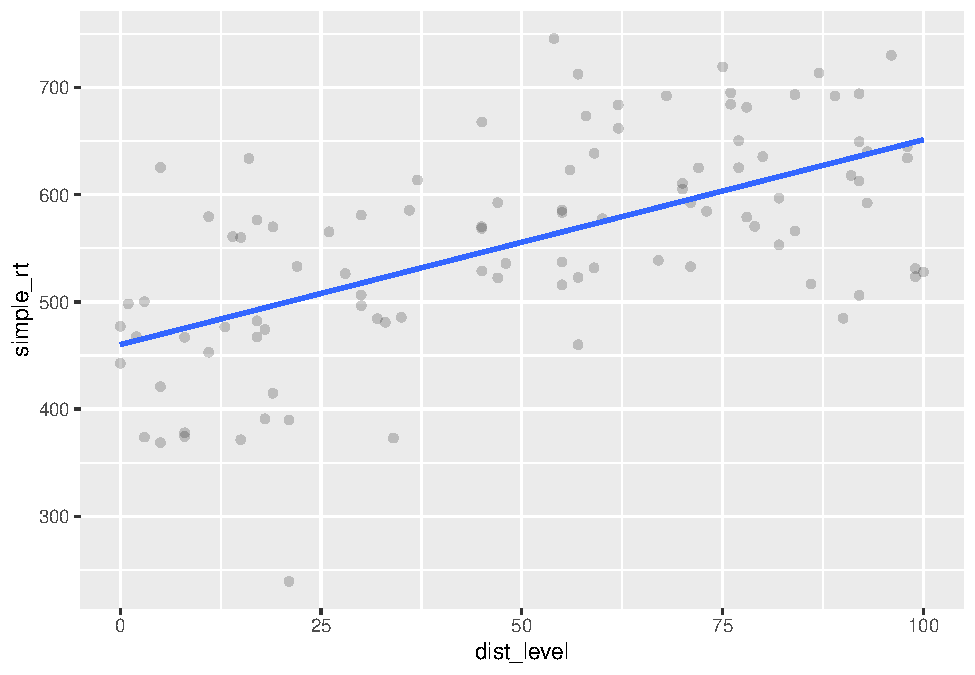
\includegraphics{04-交互效应_files/figure-latex/plot-urban-1.pdf}
\caption{\label{fig:plot-urban}\emph{声波干扰对简单反应时的影响(城市组)}}
\end{figure}

现在让我们为乡村组模拟数据。我们假设这些被试的截距可能会略高一些,可能是因为他们对技术不太熟悉。最重要的是,我们假设他们的斜率会更陡,因为他们受到噪音的影响更大。大致如下:

\[Y_i = 500 + 3 X_i + e_i\]

\begin{Shaded}
\begin{Highlighting}[]
\NormalTok{b0\_rural }\OtherTok{\textless{}{-}} \DecValTok{500}
\NormalTok{b1\_rural }\OtherTok{\textless{}{-}} \DecValTok{3}

\NormalTok{rural }\OtherTok{\textless{}{-}} \FunctionTok{tibble}\NormalTok{(}
  \AttributeTok{subj\_id =} \DecValTok{1}\SpecialCharTok{:}\NormalTok{n\_subj }\SpecialCharTok{+}\NormalTok{ n\_subj,}
  \AttributeTok{group =} \StringTok{"rural"}\NormalTok{,}
  \AttributeTok{b0 =}\NormalTok{ b0\_rural,}
  \AttributeTok{b1 =}\NormalTok{ b1\_rural,}
  \AttributeTok{dist\_level =} \FunctionTok{sample}\NormalTok{(}\DecValTok{0}\SpecialCharTok{:}\NormalTok{n\_subj, n\_subj, }\AttributeTok{replace =} \ConstantTok{TRUE}\NormalTok{),}
  \AttributeTok{err =} \FunctionTok{rnorm}\NormalTok{(n\_subj, }\AttributeTok{mean =} \DecValTok{0}\NormalTok{, }\AttributeTok{sd =} \DecValTok{80}\NormalTok{),}
  \AttributeTok{simple\_rt =}\NormalTok{ b0 }\SpecialCharTok{+}\NormalTok{ b1 }\SpecialCharTok{*}\NormalTok{ dist\_level }\SpecialCharTok{+}\NormalTok{ err)}
\end{Highlighting}
\end{Shaded}

现在让我们把这两组的数据一起画出来。

\begin{Shaded}
\begin{Highlighting}[]
\NormalTok{all\_data }\OtherTok{\textless{}{-}} \FunctionTok{bind\_rows}\NormalTok{(urban, rural)}

\FunctionTok{ggplot}\NormalTok{(all\_data }\SpecialCharTok{\%\textgreater{}\%} \FunctionTok{mutate}\NormalTok{(}\AttributeTok{group =} \FunctionTok{fct\_relevel}\NormalTok{(group, }\StringTok{"urban"}\NormalTok{)), }
       \FunctionTok{aes}\NormalTok{(dist\_level, simple\_rt, }\AttributeTok{colour =}\NormalTok{ group)) }\SpecialCharTok{+}
  \FunctionTok{geom\_point}\NormalTok{() }\SpecialCharTok{+}
  \FunctionTok{geom\_smooth}\NormalTok{(}\AttributeTok{method =} \StringTok{"lm"}\NormalTok{, }\AttributeTok{se =} \ConstantTok{FALSE}\NormalTok{) }\SpecialCharTok{+}
  \FunctionTok{facet\_wrap}\NormalTok{(}\SpecialCharTok{\textasciitilde{}}\NormalTok{ group) }\SpecialCharTok{+} 
  \FunctionTok{theme}\NormalTok{(}\AttributeTok{legend.position =} \StringTok{"none"}\NormalTok{)}
\end{Highlighting}
\end{Shaded}

\begin{figure}
\centering
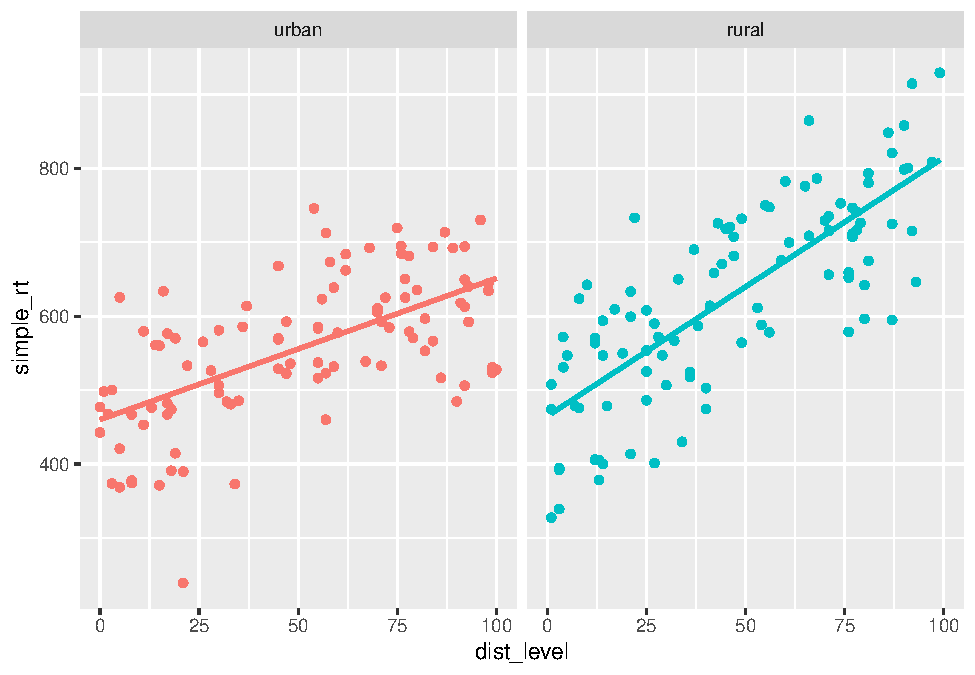
\includegraphics{04-交互效应_files/figure-latex/combined-plot-1.pdf}
\caption{\label{fig:combined-plot}\emph{声波干扰对简单反应时的影响(城市和乡村)}}
\end{figure}

这里我们可以很清楚地看到我们在数据中建立的斜率差异。我们如何测试两个斜率是否有显著不同呢?要做到这一点,我们不能做两个单独的回归。我们需要将这两条回归线纳入同一个模型中。我们应该怎么做呢?

请注意,我们可以用''偏移(offset)``值来表示其中一条回归线。我们(任意地)选一组作为我们的''基线''组,并将另一组的y轴截距和斜率表示为相对于这个基准的偏移值。因此,如果我们选择城市组作为基线,我们可以用两个偏移值\(\beta_2\)和\(\beta_3\)分别表示乡村组的y轴截距和斜率偏移。

\begin{itemize}
\tightlist
\item
  y轴截距: \(\beta_{0\_rural} = \beta_{0\_urban} + \beta_2\)
\item
  斜率: \(\beta_{1\_rural} = \beta_{1\_urban} + \beta_3\)
\end{itemize}

我们有城市组参数:\(\beta_{0\_urban} = 450\)和\(\beta_{1\_urban} = 2\),乡村组参数:\(\beta_{0\_rural} = 500\)和\(\beta_{1\_rural} = 3\)。因此可以得出:

\begin{itemize}
\tightlist
\item
  \(\beta_2 = 50\),因为\(\beta_{0\_rural} - \beta_{0\_urban} = 500 - 450 = 50\)
\item
  \(\beta_3 = 1\),因为\(\beta_{1\_rural} - \beta_{1\_urban} = 3 - 2 = 1\)
\end{itemize}

现在我们的两个回归模型是:

\[Y_{i\_urban} = \beta_{0\_urban} + \beta_{1\_urban} X_i + e_i\]

和

\[Y_{i\_rural} = (\beta_{0\_urban} + \beta_2) + (\beta_{1\_urban} + \beta_3) X_i + e_i\]

好的,看起来我们更接近将这些模型合并为一个单一的回归模型了。这里有最后的技巧。我们定义一个额外的虚拟变量,该变量在城市组中取值为0(我们选择作为''基线''组),在其他组中取值为1。下框包含我们的最终模型。

\textbf{含有连续-分类变量交互效应的回归模型}

\[Y_{i} = \beta_0 + \beta_1 X_{1i} + \beta_2 X_{2i} + \beta_3 X_{1i} X_{2i} + e_{i}\]

其中

\begin{itemize}
\tightlist
\item
  \(X_{1i}\)是连续变量
\item
  \(X_{2i}\)是虚拟变量,0表示基线组,1表示其他组
\end{itemize}

参数解释:

\begin{itemize}
\tightlist
\item
  \(\beta_0\): 基线组y轴截距;
\item
  \(\beta_1\): 基线组斜率;
\item
  \(\beta_2\): 其他组的y轴截距偏移量;
\item
  \(\beta_3\): 其他组的斜率偏移量。
\end{itemize}

用R估计:

\texttt{lm(Y\ \textasciitilde{}\ X1\ +\ X2\ +\ X1:X2,\ data)}或者简写:

\texttt{lm(Y\ \textasciitilde{}\ X1\ *\ X2,\ data)}。这里\texttt{*}的意思是:``所有可能的主效应以及X1和X2的交互''

\(\beta_3 X_{1i} X_{2i}\)项是两个预测变量相乘,被称为\textbf{交互项(interaction term)}。现在让我们展示上述广义线性模型(GLM)是如何得出两条回归线的。

为了得到城市组的回归方程,我们将0代入到\(X_{2i}\)中。得到公式:

\[Y_{i} = \beta_0 + \beta_1 X_{1i} + \beta_2 0 + \beta_3 X_{1i} 0 + e_i\]

去掉等于0的项,就得到:

\[Y_{i} = \beta_0 + \beta_1 X_{1i} + e_i,\]

这就是基线组(城市组)的回归方程。将其与上面的\(Y_{i\_urban}\)进行对比。

将1代入到\(X_{2i}\)里会得到乡村组的方程。我们得到:

\[Y_{i} = \beta_0 + \beta_1 X_{1i} + \beta_2 1 + \beta_3 X_{1i} 1 + e_i\]

化简和运用一些代数后,也能表示为:

\[Y_{i} = \beta_0 + \beta_2 + (\beta_1 + \beta_3) X_{1i} + e_i.\]

将其和上面的\(Y_{i\_rural}\)进行对比。虚拟编码起作用了!

我们如何在R中估计回归系数?假设我们想检验两条线的斜率是否不同。注意,这实际上只是检验原假设\(\beta_3 = 0\),因为\(\beta_3\)是我们的斜率偏移量。如果这个参数为0,意味着两个组具有相同的斜率(尽管它们可以有不同的截距)。换句话说,这意味着两条斜线是\textbf{平行的}。如果它非0,这意味着两个组具有不同的斜率,也就是说,两条斜线\textbf{不平行}。

\textbf{样本中的平行线 vs.~总体中的平行线}

我刚刚提到,两条不平行的线意味着分类预测变量和连续预测变量之间存在\emph{交互效应},而平行的线则意味着不存在交互效应。要明确的是,我所说的平行与否是指在总体(population)中的情况。在样本(sample)中的平行与否不仅取决于它们在总体中的情况,还取决于测量和抽样引入的偏差。总体中是平行的线,在样本中却极有可能出现斜率不同的线,尤其是在样本量较小的情况下。

通常,你会对总体中斜率相同与否感兴趣,而不是样本中的情况。因此,你不能仅仅看样本数据的图表就推断出''线不平行,因此存在交互效应'',或相反''线看起来平行,所以没有交互效应''。你必须进行推论统计检验。

当交互项在某个\(\alpha\)水平(如0.05)上具有统计显著性时,你会拒绝交互系数为0的原假设(如\(H_0: \beta_3 = 0\)),这意味着在总体中这些线不是平行的。

然而,交互项不显著并\emph{不一定}意味着在总体中这些线是平行的。它们可能是平行的,但也可能不是,而你的研究只是缺乏足够的统计效力(power)来检测出差异。

为了获得关于原假设的证据,最好的方法是进行所谓的等效性检验(equivalence test)。在这个检验中你试图拒绝一个原假设,该原假设是总体效应大于某个你感兴趣的最小效应值;教程详见\citep{Lakens_Scheel_Isager_2018}。

我们已经创建了结合两组模拟数据的数据集\texttt{all\_data}。我们使用R公式语法表示模型的方式是\texttt{Y\ \textasciitilde{}\ X1\ +\ X2\ +\ X1:X2},其中\texttt{X1:X2}告诉R创建一个预测变量,该预测变量是\texttt{X1}和\texttt{X2}的乘积。还有一个简写方式\texttt{Y\ \textasciitilde{}\ X1\ *\ X2},它告诉R计算所有可能的主效应和交互效应。首先,我们将向模型添加一个虚拟预测变量,并将结果存储在\texttt{all\_data2}中。

\begin{Shaded}
\begin{Highlighting}[]
\NormalTok{all\_data2 }\OtherTok{\textless{}{-}}\NormalTok{ all\_data }\SpecialCharTok{\%\textgreater{}\%}
  \FunctionTok{mutate}\NormalTok{(}\AttributeTok{grp =} \FunctionTok{if\_else}\NormalTok{(group }\SpecialCharTok{==} \StringTok{"rural"}\NormalTok{, }\DecValTok{1}\NormalTok{, }\DecValTok{0}\NormalTok{))}
\end{Highlighting}
\end{Shaded}

\begin{Shaded}
\begin{Highlighting}[]
\NormalTok{sonic\_mod }\OtherTok{\textless{}{-}} \FunctionTok{lm}\NormalTok{(simple\_rt }\SpecialCharTok{\textasciitilde{}}\NormalTok{ dist\_level }\SpecialCharTok{+}\NormalTok{ grp }\SpecialCharTok{+}\NormalTok{ dist\_level}\SpecialCharTok{:}\NormalTok{grp,}
\NormalTok{                all\_data2)}

\FunctionTok{summary}\NormalTok{(sonic\_mod)}
\end{Highlighting}
\end{Shaded}

\begin{verbatim}
## 
## Call:
## lm(formula = simple_rt ~ dist_level + grp + dist_level:grp, data = all_data2)
## 
## Residuals:
##      Min       1Q   Median       3Q      Max 
## -261.130  -50.749    3.617   62.304  191.211 
## 
## Coefficients:
##                Estimate Std. Error t value Pr(>|t|)    
## (Intercept)    460.1098    15.5053  29.674  < 2e-16 ***
## dist_level       1.9123     0.2620   7.299 7.07e-12 ***
## grp              4.8250    21.7184   0.222    0.824    
## dist_level:grp   1.5865     0.3809   4.166 4.65e-05 ***
## ---
## Signif. codes:  0 '***' 0.001 '**' 0.01 '*' 0.05 '.' 0.1 ' ' 1
## 
## Residual standard error: 81.14 on 196 degrees of freedom
## Multiple R-squared:  0.5625, Adjusted R-squared:  0.5558 
## F-statistic: 83.99 on 3 and 196 DF,  p-value: < 2.2e-16
\end{verbatim}

\textbf{练习}

在下面的空格中输入你的答案,至少保留两位小数。

给定回归模型

\[Y_{i} = \beta_0 + \beta_1 X_{1i} + \beta_2 X_{2i} + \beta_3 X_{1i} X_{2i} + e_{i}\]

(其中\(X_{1i}\)是连续预测变量,\(X_{2i}\)是分类预测变量)且上方给出了\texttt{lm()}的输出结果,填写以下参数的估计值。

\begin{itemize}
\tightlist
\item
  \(\hat{\beta}_0\): \_\_\_\_
\item
  \(\hat{\beta}_1\): \_\_\_\_
\item
  \(\hat{\beta}_2\): \_\_\_\_
\item
  \(\hat{\beta}_3\): \_\_\_\_
\end{itemize}

根据这些参数估计,(基线)城市组的回归线为:

\(Y_i =\) \_\_ \(+\) \_\_ \(X_{1i}\)

乡村组的:

\(Y_i =\) \_\_ \(+\) \_\_ \(X_{1i}\)

展开答案

\begin{itemize}
\tightlist
\item
  \(\beta_0=\) 460.11
\item
  \(\beta_1=\) 1.91
\item
  \(\beta_2=\) 4.83
\item
  \(\beta_3=\) 1.59
\end{itemize}

城市组的回归线是:

\(Y_i = \beta_0 + \beta_1 X_{1i}\)即

\(Y_i =\) 460.11 \(+\) 1.91 \(X_{1i}\)

乡村组的是:

\(Y_i = \beta_0 + \beta_2 + \left(\beta_1 + \beta_3\right) X_{1i}\)即

\(Y_i=\) 464.93 \(+\) 3.5 \(X_{1i}\)

\hypertarget{ux5206ux7c7bux53d8ux91cf-ux5206ux7c7bux53d8ux91cfux4ea4ux4e92ux6548ux5e94}{%
\section{分类变量-分类变量交互效应}\label{ux5206ux7c7bux53d8ux91cf-ux5206ux7c7bux53d8ux91cfux4ea4ux4e92ux6548ux5e94}}

\textbf{因子设计(factorial design)}在心理学中很常见,通常使用基于ANOVA的技术进行分析,这可能掩盖了ANOVA与回归一样也假设了一个潜在的线性模型的事实。

因子是一种所有预测变量(自变量,IVs)都是分类变量的设计:每个都是具有固定数量\textbf{水平}的\textbf{因子}。在一个全因子设计(full-factorial design)中,因子之间完全交叉,以表示每种可能的因子组合。我们称每个唯一的组合为设计的一个\textbf{单元(cell)}。你经常会听到设计被称为``二乘二(two-by-two)设计''(2x2),这意味着有2个因子,每个因子有2个水平。一个``三乘三设计''(3x3)是其中有2个因子,每个因子有3个水平的设计;一个``二乘二乘二设计''(2x2x2)是其中有3个因子,每个因子有2个水平,以此类推。

通常,因子设计都以表格形式给出,显示所有因子水平的组合。下面是一个2x2设计的表格表示。

\begin{table}
\centering
\begin{tabular}{l|l|l}
\hline
  & \$B\_1\$ & \$B\_2\$\\
\hline
\$A\_1\$ & \$AB\_\{11\}\$ & \$AB\_\{12\}\$\\
\hline
\$A\_2\$ & \$AB\_\{21\}\$ & \$AB\_\{22\}\$\\
\hline
\end{tabular}
\end{table}

一个3x2设计可能如下所示。

\begin{table}
\centering
\begin{tabular}{l|l|l}
\hline
  & \$B\_1\$ & \$B\_2\$\\
\hline
\$A\_1\$ & \$AB\_\{11\}\$ & \$AB\_\{12\}\$\\
\hline
\$A\_2\$ & \$AB\_\{21\}\$ & \$AB\_\{22\}\$\\
\hline
\$A\_3\$ & \$AB\_\{31\}\$ & \$AB\_\{32\}\$\\
\hline
\end{tabular}
\end{table}

最后是一个2x2x2设计.

\[C_1\]

\begin{table}
\centering
\begin{tabular}{l|l|l}
\hline
  & \$B\_1\$ & \$B\_2\$\\
\hline
\$A\_1\$ & \$ABC\_\{111\}\$ & \$ABC\_\{121\}\$\\
\hline
\$A\_2\$ & \$ABC\_\{211\}\$ & \$ABC\_\{221\}\$\\
\hline
\end{tabular}
\end{table}

\[C_2\]

\begin{table}
\centering
\begin{tabular}{l|l|l}
\hline
  & \$B\_1\$ & \$B\_2\$\\
\hline
\$A\_1\$ & \$ABC\_\{112\}\$ & \$ABC\_\{122\}\$\\
\hline
\$A\_2\$ & \$ABC\_\{212\}\$ & \$ABC\_\{222\}\$\\
\hline
\end{tabular}
\end{table}

不要混淆\textbf{因子}和\textbf{水平}!

如果你听说一个研究有三个处理组(处理组A、处理组B和对照组),这不是一个``三因子(three-factor, three-way)设计''。这是一个单因子(one-factor, one-way)设计,具有一个三水平因子(处理条件)。

不存在只有一个水平的因子。

你可以通过将每个因子的水平数相乘来确定设计中有多少个单元。因此,一个2x3x4设计将在设计中有24个单元。

\hypertarget{ux8ba4ux77e5ux6cbbux7597ux4e0eux836fux7269ux6cbbux7597ux5bf9ux60c5ux7eeaux7684ux5f71ux54cd}{%
\subsection{认知治疗与药物治疗对情绪的影响}\label{ux8ba4ux77e5ux6cbbux7597ux4e0eux836fux7269ux6cbbux7597ux5bf9ux60c5ux7eeaux7684ux5f71ux54cd}}

让我们考虑一个简单的因子设计,并思考我们的数据可能展示方式。在从这个具体例子中了解概念之后,我们将将其映射到更抽象的统计术语上。

想象一下,你正在进行一项研究,内容是两种不同类型的治疗(认知疗法和药物疗法)对抑郁症患者的影响。一半的被试被随机分配接受认知行为疗法(Cognitive Behavioral Therapy, CBT),另一半接受其他控制操作(no-CBT)。此外,你通过随机分配进一步将你的患者分为两组:药物治疗组(接受抗抑郁药物, drug)和对照组(接受安慰剂, placebo)。接受治疗(或对照/安慰剂)后,你使用一个评分标准来测量他们的情绪,较高的数字对应较积极的情绪。

让我们想象一下,下面我们得到的均值是不受测量或抽样误差影响的总体均值。我们将花一点时间考虑3种不同的可能结果,以及它们暗示这些疗法如何独立或交互地影响情绪。

在分类变量-连续变量交互效应部分关于的总体和样本的提醒在这里同样适用。除非模拟数据,你几乎\textbf{永远不会}知道你正在研究的任何总体的真实均值。下面,我们讨论的是你实际知道总体均值并且可以在没有任何统计测试的情况下得出结论的假设情况。你观察到的任何真实样本均值都会包含抽样和测量误差,你所做的任何推断都将取决于统计检验的结果,而不是观察到的均值。

\hypertarget{ux60c5ux666fa}{%
\subsubsection*{情景A}\label{ux60c5ux666fa}}
\addcontentsline{toc}{subsubsection}{情景A}

\begin{figure}
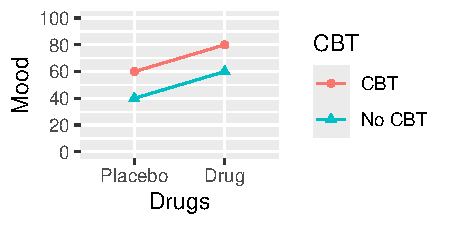
\includegraphics[width=0.5\linewidth]{04-交互效应_files/figure-latex/scenario-a-plot-1} \caption{*情景A, 单元平均值图*}\label{fig:scenario-a-plot}
\end{figure}

下面是一个\textbf{单元均值(cell mean)}和\textbf{边际均值(marginal mean)}的表格。单元均值是设计的每个单元中因变量(情绪)的平均值。边际均值(在表格的边缘)提供了每行和每列的均值。

\begin{table}
\centering
\begin{tabular}{l|r|r|l}
\hline
  & No CBT & CBT &   \\
\hline
Placebo & 40 & 60 & 50\\
\hline
Drug & 60 & 80 & 70\\
\hline
 & 50 & 70 & \\
\hline
\end{tabular}
\end{table}

如果这是我们的结果,你会得出什么结论?认知疗法对情绪有影响吗?药物疗法呢?对于这两个问题的答案都是肯定的:接受CBT的人平均心情(70;第2列的均值)比没有接受的人高出20(50;第1列的均值)。

同样,接受抗抑郁药物的人情绪(70;第2行均值)相对于接受安慰剂的人(50; 第1行均值)更好。

现在我们还可以问下个问题:\textbf{认知疗法的效果是否取决于患者是否同时接受药物疗法}?答案是否定的。看看为什么,注意到对于安慰剂组(第1行),认知疗法使情绪提高了20分(从40提高到60)。但对于药物组来说也是一样的:从60提高到80也是20分的提高。因此,没有证据表明一个因素对心情的影响取决于另一个因素。

\hypertarget{ux60c5ux666fb}{%
\subsubsection*{情景B}\label{ux60c5ux666fb}}
\addcontentsline{toc}{subsubsection}{情景B}

\begin{figure}
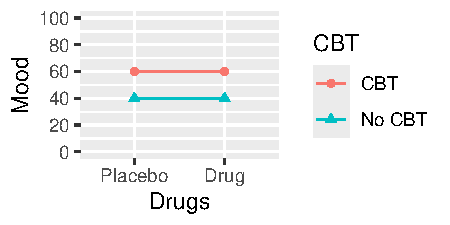
\includegraphics[width=0.5\linewidth]{04-交互效应_files/figure-latex/scenario-b-plot-1} \caption{*情景B, 单元平均值图*}\label{fig:scenario-b-plot}
\end{figure}

\begin{table}
\centering
\begin{tabular}{l|r|r|l}
\hline
  & No CBT & CBT &   \\
\hline
Placebo & 40 & 60 & 50\\
\hline
Drug & 40 & 60 & 50\\
\hline
 & 40 & 60 & \\
\hline
\end{tabular}
\end{table}

在这种情景下,我们也发现CBT改善了情绪(同样提高了20分),但药物疗法没有效果(第1行和第2行的边际均值都是50)。我们还可以看到,CBT的效果也不依赖于药物疗法:每行都有20分的提高。

\hypertarget{ux60c5ux666fc}{%
\subsubsection*{情景C}\label{ux60c5ux666fc}}
\addcontentsline{toc}{subsubsection}{情景C}

\begin{figure}
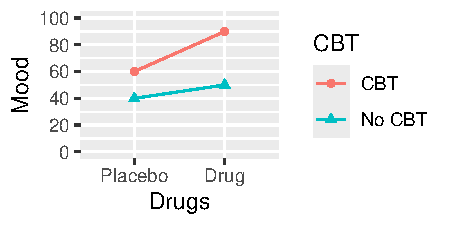
\includegraphics[width=0.5\linewidth]{04-交互效应_files/figure-latex/scenario-c-plot-1} \caption{*情景C, 单元平均值图*}\label{fig:scenario-c-plot}
\end{figure}

\begin{table}
\centering
\begin{tabular}{l|r|r|l}
\hline
  & No CBT & CBT &   \\
\hline
Placebo & 40 & 60 & 50\\
\hline
Drug & 50 & 90 & 70\\
\hline
 & 45 & 75 & \\
\hline
\end{tabular}
\end{table}

根据前面的逻辑,我们发现总体上接受认知疗法的人相比于对照组,情绪有所提升(75分对45分),而接受药物疗法的人相比于安慰剂组,情绪也有所提升(70分对50分)。但这里还有其他情况:认知疗法对情绪的影响\textbf{在同时接受药物疗法的患者中更明显}。对于服用抗抑郁药的患者,情绪相对于对照组提高了40分(从50分到90分;表中的第2行)。对于接受安慰剂的患者,情绪只提高了20分,从40分到60分(表中的第1行)。因此,在这个假设情景中,\textbf{认知疗法的效果取决于是否同时进行药物疗法}。

\hypertarget{ux56e0ux5b50ux8bbeux8ba1ux4e2dux7684ux6548ux5e94}{%
\subsection{因子设计中的效应}\label{ux56e0ux5b50ux8bbeux8ba1ux4e2dux7684ux6548ux5e94}}

如果你理解了上一节描述的基本效应模式,那么你就准备好将这些概念映射到统计语言上了。

\hypertarget{ux4e3bux6548ux5e94main-effect}{%
\subsubsection{主效应(main effect)}\label{ux4e3bux6548ux5e94main-effect}}

\textbf{主效应}:在\textbf{忽略}设计中其他因子的情况下,一个因子对因变量的效应。

主效应的检验是对边际均值是否等价的检验。因此,在上述场景A中,当你比较药物治疗的行均值时,你是在评估该因子对情绪的主效应。原假设是这两个边际均值相等:

\[\bar{Y}_{1..} = \bar{Y}_{2..}\]

其中\(Y_{i..}\)是不考虑列因子的情况下\(i\)行的平均值。

如果你有一个因子有\(k\)水平,且\(k > 2\),此时主效应的原假设是:

\[\bar{Y}_{1..} = \bar{Y}_{2..} = \ldots = \bar{Y}_{k..},\]

即所有的行(或列)都是相等的。

\hypertarget{ux7b80ux5355ux6548ux5e94simple-effect}{%
\subsubsection{简单效应(simple effect)}\label{ux7b80ux5355ux6548ux5e94simple-effect}}

\textbf{简单效应}是指在另一个因子的特定水平上(将该因子保持在特定值),一个因子的效应。

例如,在情景C中,我们讨论了CBT对抗抑郁药组被试的效应。在这种情况下,对于接受抗抑郁药的被试来说,CBT的简单效应是40个单位。

我们也可以讨论药物治疗对接受认知疗法的患者的简单效应。在情景C中,这体现为情绪得分从60增加到90(第2列)。

\hypertarget{ux4ea4ux4e92ux6548ux5e94-1}{%
\subsubsection{交互效应}\label{ux4ea4ux4e92ux6548ux5e94-1}}

当一个变量的效应在另一个变量的各个水平上不同的时候,我们称之为存在\textbf{交互效应}。

更像数学定义的表述是,当一个因子的简单效应在另一个因子的各个水平上不同时,就存在交互效应。我们在情景C中看到了这一点,CBT对抗抑郁药组的效果提升了40个单位,而对安慰剂组的效果只提升了20个单位。也许抗抑郁药带来的情绪提升使患者更容易接受CBT。

关键在于,当A的简单效应在B的各个水平上不同时,我们称A和B之间存在简单交互效应。你也可以检查B的简单效应在A上是否不同。如果其中一个陈述为真,另一个陈述也必为真,因此查看简单效应的方式并不重要。

\hypertarget{ux9ad8ux9636ux8bbeux8ba1higher-order-designs}{%
\subsection{高阶设计(Higher-order designs)}\label{ux9ad8ux9636ux8bbeux8ba1higher-order-designs}}

双因子设计(也称为``two-way'')在心理学和神经科学中非常常见,但有时你也会遇到超过两个因子的设计,比如2x2x2设计。

为了计算不同类型效应的数量,我们使用下面的公式,这个公式给出了从\(n\)个元素中取\(k\)个元素的可能组合数:

\[\frac{n!}{k!(n - k)!}\]

相比于实际上的手算,我们可以在R中使用\texttt{choose(n,\ k)}函数。

对于有\(n\)个因子的设计,你会有:

\begin{itemize}
\tightlist
\item
  \(n\)个主效应;
\item
  \(\frac{n!}{2!(n - 2)!}\)个2因素交互效应;
\item
  \(\frac{n!}{3!(n - 3)!}\)个3因素交互效应;
\item
  \(\frac{n!}{4!(n - 4)!}\)个4因素交互效应\ldots 以此类推。
\end{itemize}

因此,如果我们有一个3因子设计,如一个2x2x2设计,其中包含因子\(A\),\(B\)和\(C\),我们将有3个主效应:\(A\),\(B\)和\(C\);\texttt{choose(3,\ 2)} = 3个2因素交互效应:\(AB\),\(AC\)和\(BC\),以及\texttt{choose(3,\ 3)} = 1个3因素交互效应:\(ABC\)。

3因素交互效应很难解释,但它们意味着任意两个给定因子之间的\textbf{简单交互效应}会随着第3个因子的水平变化而不同。例如,它可能意味着\(C_1\)处的\(AB\)交互效应与\(C_2\)处的\(AB\)交互效应不同。

如果你有一个4因子设计,你将会有四个主效应,\texttt{choose(4,\ 2)} = 6个2因素交互效应,\texttt{choose(4,\ 3)} = 4个3因素交互效应,以及1个4因素交互效应。从4因子设计中解释结果几乎是不可能的,所以请保持你的设计简单!

\textbf{常见错误}

比较简单效应的显著性\textbf{不等于}检验简单效应是否有显著差异。

\hypertarget{ux7528ux4e8eux56e0ux5b50ux8bbeux8ba1ux7684glm}{%
\section{用于因子设计的GLM}\label{ux7528ux4e8eux56e0ux5b50ux8bbeux8ba1ux7684glm}}

现在让我们看一下这些模型背后的数学。通常情况下,你会看到为2x2因子设计编写的方差分析(ANOVA)的GLM使用``ANOVA''符号,如下所示:

\[Y_{ijk} = \mu + A_i + B_j + AB_{ij} + S(AB)_{ijk}.\]

在上方公式中:

\begin{itemize}
\tightlist
\item
  \(Y_{ijk}\)表示在因子\(A\)的第\(i\)个水平和因子\(B\)的第\(j\)个水平中观测到的\(k\)的值;
\item
  \(\mu\)表示总体均值;
\item
  \(A_i\)表示因子\(A\)在\(A\)的第\(i\)个水平上的主效应;
\item
  \(B_j\)表示因子\(B\)在\(B\)的第\(j\)个水平上的主效应;
\item
  \(AB_{ij}\)表示在\(A\)的第\(i\)个水平和\(B\)的第\(j\)个水平处的\(AB\)交互效应;
\item
  \(S(AB)_{ijk}\)表示残差。
\end{itemize}

一个重要的数学事实是,各个主效应和交互效应的总和为零,通常写成:

\begin{itemize}
\tightlist
\item
  \(\Sigma_i A_i = 0\);
\item
  \(\Sigma_j B_j = 0\);
\item
  \(\Sigma_{ij} AB_{ij} = 0\)。
\end{itemize}

理解这些效应的最好方法是查看分解表。研究下面的分解表,该表包含了从具有因子\(A\)和\(B\)的2x2设计中获取的12个模拟观测值。提供了索引\(i\)、\(j\)和\(k\),只是为了帮助你跟踪正在处理的观测值。请记住,\(i\)表示因子\(A\)的水平,\(j\)表示因子\(B\)的水平,\(k\)表示单元\(AB_{ij}\)内的观测值编号。

\begin{verbatim}
## # A tibble: 12 x 9
##        Y     i     j     k    mu   A_i   B_j AB_ij   err
##    <dbl> <int> <int> <int> <dbl> <dbl> <dbl> <dbl> <int>
##  1    11     1     1     1    10     4    -2    -1     0
##  2    14     1     1     2    10     4    -2    -1     3
##  3     8     1     1     3    10     4    -2    -1    -3
##  4    17     1     2     1    10     4     2     1     0
##  5    15     1     2     2    10     4     2     1    -2
##  6    19     1     2     3    10     4     2     1     2
##  7     8     2     1     1    10    -4    -2     1     3
##  8     4     2     1     2    10    -4    -2     1    -1
##  9     3     2     1     3    10    -4    -2     1    -2
## 10    10     2     2     1    10    -4     2    -1     3
## 11     7     2     2     2    10    -4     2    -1     0
## 12     4     2     2     3    10    -4     2    -1    -3
\end{verbatim}

\hypertarget{ux4f30ux8ba1ux65b9ux7a0bestimation-equations}{%
\subsection{估计方程(estimation equations)}\label{ux4f30ux8ba1ux65b9ux7a0bestimation-equations}}

这些是你在ANOVA中用来估计效应的方程。

\begin{itemize}
\tightlist
\item
  \(\hat{\mu} = Y_{...}\)
\item
  \(\hat{A}_i = Y_{i..} - \hat{\mu}\)
\item
  \(\hat{B}_j = Y_{.j.} - \hat{\mu}\)
\item
  \(\widehat{AB}_{ij} = Y_{ij.} - \hat{\mu} - \hat{A}_i - \hat{B}_j\)
\end{itemize}

注意,带有下标点的\(Y\)变量是\(Y\)的均值,忽略了下标中的任何内容。因此,\(Y_{...}\)是\(Y\)的均值,\(Y_{i..}\)是\(Y\)在\(A\)的第\(i\)个水平上的均值,\(Y_{.j.}\)是\(Y\)在\(B\)的第\(j\)个水平上的均值,\(Y_{ij.}\)是\(Y\)在\(A\)的第\(i\)个水平和\(B\)的第\(j\)个水平上的均值,即单元均值\(ij\)。

\hypertarget{ux56e0ux5b50ux8bbeux8ba1app}{%
\subsection{因子设计App}\label{ux56e0ux5b50ux8bbeux8ba1app}}

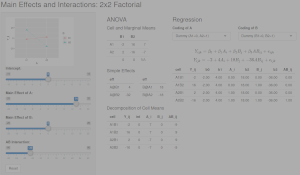
\includegraphics{images/04-interactions_factorial_app.png}

\href{https://rstudio-connect.psy.gla.ac.uk/factorial}{启动这个网页APP},尝试因子设计,直到你理解因子设计中主效应和交互效应的关键概念。

\hypertarget{ux5728ux56e0ux5b50ux8bbeux8ba1ux4e2dux5bf9ux5206ux7c7bux9884ux6d4bux56e0ux5b50ux8fdbux884cux7f16ux7801}{%
\section{在因子设计中对分类预测因子进行编码}\label{ux5728ux56e0ux5b50ux8bbeux8ba1ux4e2dux5bf9ux5206ux7c7bux9884ux6d4bux56e0ux5b50ux8fdbux884cux7f16ux7801}}

心理学研究(尤其是实验心理学)经常涉及分类自变量。分析这些研究的数据时,需要仔细指定预测变量,因为R中的默认设置对实验情景而言并不理想。主要问题是分类预测变量的默认编码在输出中给出的是\textbf{简单效应}而非\textbf{主效应},但后者通常是你所需要的。人们有时没有意识到这一点,误读了他们的输出结果。研究人员有时会报告含有分类预测变量的回归结果,但未明确报告他们是如何编码这些变量的,这使得他们的研究结果难以解读和再现。为了确保可重复性、透明度和准确解释,学习如何``手动''编码分类预测变量并在报告中习惯性地报告这些编码是一个好主意。

由于R的默认设置不适合因子设计,我建议在将分类变量作为线性模型中的预测变量时,应该总是手动编码分类变量。不要将它们包括为\texttt{factor}变量。

\hypertarget{ux5206ux7c7bux53d8ux91cfux7684ux7f16ux7801ux65b9ux6848}{%
\section{分类变量的编码方案}\label{ux5206ux7c7bux53d8ux91cfux7684ux7f16ux7801ux65b9ux6848}}

许多实验研究者在尝试从方差分析(ANOVA)转向使用R进行线性混合效应模型(linear mixed-effects models,LMEMs)时,都会在编码分类预测变量时遇到困难。这比预期的要复杂得多,而R提供的默认设置对于因子实验来说完全不合适。实际上,在因子实验中使用这些默认设置可能会导致研究人员从数据中得出错误的结论。

为了简化问题,我们将从设计因子不超过两水平的情况开始,然后再讨论具有三个以上水平的设计。

\hypertarget{ux7b80ux5355ux6548ux5e94-vs.-ux4e3bux6548ux5e94}{%
\subsection{简单效应 vs.~主效应}\label{ux7b80ux5355ux6548ux5e94-vs.-ux4e3bux6548ux5e94}}

理解\textbf{简单效应(simple effect)}和\textbf{主效应(main effect)}以及\textbf{简单交互效应(simple interaction)}和\textbf{主交互效应(main interaction)}在三因素设计中的区别是非常重要的。

在\(A{\times}B\)设计中,\(A\)的简单效应是\textbf{控制}\(B\)后的\(A\)的效应,而\(A\)的主效应是\textbf{忽略}\(B\)后\(A\)的效应。另一种看待这个问题的方法是考虑因子设计中的单元均值(\(\bar{Y}_{11}\),\(\bar{Y}_{12}\),\(\bar{Y}_{21}\)和\(\bar{Y}_{22}\))以及边际均值(\(\bar{Y}_{1.}\),\(\bar{Y}_{2.}\),\(\bar{Y}_{.1}\)和\(\bar{Y}_{.2}\))。(下标的点告诉你``忽略''该点的维度;例如:\(\bar{Y}_{.1}\)告诉你忽略行变量取第1列的均值)。测试\(A\)的主效应是测试原假设\(\bar{Y}_{1.}=\bar{Y}_{2.}\)。测试\(A\)的简单效应,即在\(B\)的特定水平上\(A\)的效应,例如,测试原假设\(\bar{Y}_{11}=\bar{Y}_{21}\)。

\begin{table}
\centering
\begin{tabular}{c|c|c|c|c}
\hline
 & \textbackslash{}(B\_1\textbackslash{}) & \textbackslash{}(B\_2\textbackslash{}) &  & \\
\hline
\textbackslash{}(A\_1\textbackslash{}) & \$\textbackslash{}bar\{Y\}\_\{11\}\$ & \$\textbackslash{}bar\{Y\}\_\{12\}\$ &  & \$\textbackslash{}bar\{Y\}\_\{1.\}\$\\
\hline
\textbackslash{}(A\_2\textbackslash{}) & \$\textbackslash{}bar\{Y\}\_\{21\}\$ & \$\textbackslash{}bar\{Y\}\_\{22\}\$ &  & \$\textbackslash{}bar\{Y\}\_\{2.\}\$\\
\hline
 &  &  &  & \\
\hline
 & \$\textbackslash{}bar\{Y\}\_\{.1\}\$ & \$\textbackslash{}bar\{Y\}\_\{.2\}\$ &  & \\
\hline
\end{tabular}
\end{table}

区别\textbf{简单交互效应}和\textbf{主交互效应}的逻辑相同:在\(ABC\)设计中,\(AB\)的简单交互效应是在\(C\)的特定水平上\(AB\)交互效应;而\(AB\)的主交互效应是\textbf{忽略}\(C\)后\(AB\)的交互效应。后者是我们在三因子设计中通常讨论的低阶交互效应(lower-order interaction)。这也是标准ANOVA程序(如R的\texttt{aov()}函数、SPSS、SAS等)输出中所提供的内容。

\hypertarget{ux4e3bux8981ux7f16ux7801ux65b9ux6848}{%
\subsection{主要编码方案}\label{ux4e3bux8981ux7f16ux7801ux65b9ux6848}}

通常,编码方案的选择会影响对数据的解释:

\begin{enumerate}
\def\labelenumi{\arabic{enumi}.}
\tightlist
\item
  截距项的解释
\item
  因子设计中除最高阶效应和(最高阶)交互效应之外的所有测试的解释。
\end{enumerate}

它还会影响混合效应模型中随机效应的解释/估计(详见这篇\href{https://talklab.psy.gla.ac.uk/simgen/rsonly.html}{博客})。如果你的设计只有一个两水平因素,并且使用了\href{https://www.sciencedirect.com/science/article/pii/S0749596X12001180}{最大随机效应结构}( maximal random-effects structure),那么编码方案的选择实际上并不重要。

有许多可能的编码方案(详见\texttt{?contr.treatment})。最相关的编码方案是\textbf{处理(treatment)编码}、\textbf{求和(sum)编码}和\textbf{偏差(deviation)编码}。求和编码和偏差编码可以被视为\textbf{效应编码(effect coding)}的特例------人们通常把那些编码总和为0的编码称为效应编码。

对于2水平因子,你可以使用下面代码:

\begin{table}
\centering
\begin{tabular}{l|r|r}
\hline
Scheme & \textbackslash{}(A\_1\textbackslash{}) & \textbackslash{}(A\_2\textbackslash{})\\
\hline
Treatment (dummy) & \textbackslash{}(0\textbackslash{}) & \textbackslash{}(1\textbackslash{})\\
\hline
Sum & \textbackslash{}(-1\textbackslash{}) & \textbackslash{}(1\textbackslash{})\\
\hline
Deviation & \textbackslash{}(-\textbackslash{}frac\{1\}\{2\}\textbackslash{}) & \textbackslash{}(\textbackslash{}frac\{1\}\{2\}\textbackslash{})\\
\hline
\end{tabular}
\end{table}

默认情况下,R对模型中定义为=factor=的任何变量使用处理编码(详见\texttt{?factor}和\texttt{?contrasts})。要了解为什么这对因子设计而言并不理想,可以考虑一个2x2x2的因子设计,因子包括\(A\)、\(B\) 和\(C\)。我们将只考虑一个完全的被试内设计,每个被试只有一个观测值,因为这允许我们使用最简单的可能的误差结构(error structure)。我们将使用\texttt{lm()}来拟合一个这样的模型:

\texttt{lm(Y\ \textasciitilde{}\ A\ *\ B\ *\ C)}

下图详细说明了2x2x2设计的各种单元均值和边际均值的符号。

\[C_1\]

\begin{table}
\centering
\begin{tabular}{c|c|c|c|c}
\hline
 & \textbackslash{}(B\_1\textbackslash{}) & \textbackslash{}(B\_2\textbackslash{}) &  & \\
\hline
\textbackslash{}(A\_1\textbackslash{}) & \$\textbackslash{}bar\{Y\}\_\{111\}\$ & \$\textbackslash{}bar\{Y\}\_\{121\}\$ &  & \$\textbackslash{}bar\{Y\}\_\{1.1\}\$\\
\hline
\textbackslash{}(A\_2\textbackslash{}) & \$\textbackslash{}bar\{Y\}\_\{211\}\$ & \$\textbackslash{}bar\{Y\}\_\{221\}\$ &  & \$\textbackslash{}bar\{Y\}\_\{2.1\}\$\\
\hline
 &  &  &  & \\
\hline
 & \$\textbackslash{}bar\{Y\}\_\{.11\}\$ & \$\textbackslash{}bar\{Y\}\_\{.21\}\$ &  & \\
\hline
\end{tabular}
\end{table}

\[C_2\]

\begin{table}
\centering
\begin{tabular}{c|c|c|c|c}
\hline
 & \textbackslash{}(B\_1\textbackslash{}) & \textbackslash{}(B\_2\textbackslash{}) &  & \\
\hline
\textbackslash{}(A\_1\textbackslash{}) & \$\textbackslash{}bar\{Y\}\_\{112\}\$ & \$\textbackslash{}bar\{Y\}\_\{122\}\$ &  & \$\textbackslash{}bar\{Y\}\_\{1.2\}\$\\
\hline
\textbackslash{}(A\_2\textbackslash{}) & \$\textbackslash{}bar\{Y\}\_\{212\}\$ & \$\textbackslash{}bar\{Y\}\_\{222\}\$ &  & \$\textbackslash{}bar\{Y\}\_\{2.2\}\$\\
\hline
 &  &  &  & \\
\hline
 & \$\textbackslash{}bar\{Y\}\_\{.12\}\$ & \$\textbackslash{}bar\{Y\}\_\{.22\}\$ &  & \\
\hline
\end{tabular}
\end{table}

下表提供了在三种不同编码方案下模型中各种效应的解释。注意,\(Y\)是因变量,下标的点表示``忽略''相应的维度。因此,\(\bar{Y}_{.1.}\)是B\_1的均值(忽略因子\(A\)和因子\(C\)),而\(\bar{Y}_{...}\)是``总均值''(忽略所有因子)。

\begin{table}
\centering
\begin{tabular}{c|c|c|c}
\hline
term & treatment & sum & deviation\\
\hline
\textbackslash{}(\textbackslash{}mu\textbackslash{}) & \$\textbackslash{}bar\{Y\}\_\{111\}\$ & \$\textbackslash{}bar\{Y\}\_\{...\}\$ & \$\textbackslash{}bar\{Y\}\_\{...\}\$\\
\hline
\textbackslash{}(A\textbackslash{}) & \textbackslash{}(\textbackslash{}bar\{Y\}\_\{211\} - \textbackslash{}bar\{Y\}\_\{111\}\textbackslash{}) & \textbackslash{}(\textbackslash{}frac\{(\textbackslash{}bar\{Y\}\_\{2..\} - \textbackslash{}bar\{Y\}\_\{1..\})\}\{2\}\textbackslash{}) & \textbackslash{}(\textbackslash{}bar\{Y\}\_\{2..\} - \textbackslash{}bar\{Y\}\_\{1..\}\textbackslash{})\\
\hline
\textbackslash{}(B\textbackslash{}) & \textbackslash{}(\textbackslash{}bar\{Y\}\_\{121\} - \textbackslash{}bar\{Y\}\_\{111\}\textbackslash{}) & \textbackslash{}(\textbackslash{}frac\{(\textbackslash{}bar\{Y\}\_\{.2.\} - \textbackslash{}bar\{Y\}\_\{.1.\})\}\{2\}\textbackslash{}) & \textbackslash{}(\textbackslash{}bar\{Y\}\_\{.2.\} - \textbackslash{}bar\{Y\}\_\{.1.\}\textbackslash{})\\
\hline
\textbackslash{}(C\textbackslash{}) & \textbackslash{}(\textbackslash{}bar\{Y\}\_\{112\} - \textbackslash{}bar\{Y\}\_\{111\}\textbackslash{}) & \textbackslash{}(\textbackslash{}frac\{(\textbackslash{}bar\{Y\}\_\{..2\} - \textbackslash{}bar\{Y\}\_\{..1\})\}\{2\}\textbackslash{}) & \textbackslash{}(\textbackslash{}bar\{Y\}\_\{..2\} - \textbackslash{}bar\{Y\}\_\{..1\}\textbackslash{})\\
\hline
\textbackslash{}(AB\textbackslash{}) & \textbackslash{}((\textbackslash{}bar\{Y\}\_\{221\} - \textbackslash{}bar\{Y\}\_\{121\}) - (\textbackslash{}bar\{Y\}\_\{211\} - \textbackslash{}bar\{Y\}\_\{111\})\textbackslash{}) & \textbackslash{}(\textbackslash{}frac\{(\textbackslash{}bar\{Y\}\_\{22.\} - \textbackslash{}bar\{Y\}\_\{12.\}) - (\textbackslash{}bar\{Y\}\_\{21.\} - \textbackslash{}bar\{Y\}\_\{11.\})\}\{4\}\textbackslash{}) & \textbackslash{}((\textbackslash{}bar\{Y\}\_\{22.\} - \textbackslash{}bar\{Y\}\_\{12.\}) - (\textbackslash{}bar\{Y\}\_\{21.\} - \textbackslash{}bar\{Y\}\_\{11.\})\textbackslash{})\\
\hline
\textbackslash{}(AC\textbackslash{}) & \textbackslash{}((\textbackslash{}bar\{Y\}\_\{212\} - \textbackslash{}bar\{Y\}\_\{211\}) - (\textbackslash{}bar\{Y\}\_\{112\} - \textbackslash{}bar\{Y\}\_\{111\})\textbackslash{}) & \textbackslash{}(\textbackslash{}frac\{(\textbackslash{}bar\{Y\}\_\{2.2\} - \textbackslash{}bar\{Y\}\_\{1.2\}) - (\textbackslash{}bar\{Y\}\_\{2.1\} - \textbackslash{}bar\{Y\}\_\{1.1\})\}\{4\}\textbackslash{}) & \textbackslash{}((\textbackslash{}bar\{Y\}\_\{2.2\} - \textbackslash{}bar\{Y\}\_\{1.2\}) - (\textbackslash{}bar\{Y\}\_\{2.1\} - \textbackslash{}bar\{Y\}\_\{1.1\})\textbackslash{})\\
\hline
\textbackslash{}(BC\textbackslash{}) & \textbackslash{}((\textbackslash{}bar\{Y\}\_\{122\} - \textbackslash{}bar\{Y\}\_\{112\}) - (\textbackslash{}bar\{Y\}\_\{121\} - \textbackslash{}bar\{Y\}\_\{111\})\textbackslash{}) & \textbackslash{}(\textbackslash{}frac\{(\textbackslash{}bar\{Y\}\_\{.22\} - \textbackslash{}bar\{Y\}\_\{.12\}) - (\textbackslash{}bar\{Y\}\_\{.21\} - \textbackslash{}bar\{Y\}\_\{.11\})\}\{4\}\textbackslash{}) & \textbackslash{}((\textbackslash{}bar\{Y\}\_\{.22\} - \textbackslash{}bar\{Y\}\_\{.12\}) - (\textbackslash{}bar\{Y\}\_\{.21\} - \textbackslash{}bar\{Y\}\_\{.11\})\textbackslash{})\\
\hline
\end{tabular}
\end{table}

对于三因子\(A \times B \times C\)的交互效应:

\begin{table}
\centering
\begin{tabular}{c|c}
\hline
scheme & interpretation\\
\hline
treatment & \textbackslash{}(\textbackslash{}displaystyle\textbackslash{}left[\textbackslash{}displaystyle\textbackslash{}left(\textbackslash{}bar\{Y\}\_\{221\} - \textbackslash{}bar\{Y\}\_\{121\}\textbackslash{}right) - \textbackslash{}displaystyle\textbackslash{}left(\textbackslash{}bar\{Y\}\_\{211\} - \textbackslash{}bar\{Y\}\_\{111\}\textbackslash{}right)\textbackslash{}right] - \textbackslash{}displaystyle\textbackslash{}left[\textbackslash{}displaystyle\textbackslash{}left(\textbackslash{}bar\{Y\}\_\{222\} - \textbackslash{}bar\{Y\}\_\{122\}\textbackslash{}right) - \textbackslash{}displaystyle\textbackslash{}left(\textbackslash{}bar\{Y\}\_\{212\} - \textbackslash{}bar\{Y\}\_\{112\}\textbackslash{}right)\textbackslash{}right]\textbackslash{})\\
\hline
sum & \textbackslash{}(\textbackslash{}frac\{\textbackslash{}displaystyle\textbackslash{}left[\textbackslash{}displaystyle\textbackslash{}left(\textbackslash{}bar\{Y\}\_\{221\} - \textbackslash{}bar\{Y\}\_\{121\}\textbackslash{}right) - \textbackslash{}displaystyle\textbackslash{}left(\textbackslash{}bar\{Y\}\_\{211\} - \textbackslash{}bar\{Y\}\_\{111\}\textbackslash{}right)\textbackslash{}right] - \textbackslash{}displaystyle\textbackslash{}left[\textbackslash{}displaystyle\textbackslash{}left(\textbackslash{}bar\{Y\}\_\{222\} - \textbackslash{}bar\{Y\}\_\{122\}\textbackslash{}right) - \textbackslash{}displaystyle\textbackslash{}left(\textbackslash{}bar\{Y\}\_\{212\} - \textbackslash{}bar\{Y\}\_\{112\}\textbackslash{}right)\textbackslash{}right]\}\{8\}\textbackslash{})\\
\hline
deviation & \textbackslash{}(\textbackslash{}displaystyle\textbackslash{}left[\textbackslash{}displaystyle\textbackslash{}left(\textbackslash{}bar\{Y\}\_\{221\} - \textbackslash{}bar\{Y\}\_\{121\}\textbackslash{}right) - \textbackslash{}displaystyle\textbackslash{}left(\textbackslash{}bar\{Y\}\_\{211\} - \textbackslash{}bar\{Y\}\_\{111\}\textbackslash{}right)\textbackslash{}right] - \textbackslash{}displaystyle\textbackslash{}left[\textbackslash{}displaystyle\textbackslash{}left(\textbackslash{}bar\{Y\}\_\{222\} - \textbackslash{}bar\{Y\}\_\{122\}\textbackslash{}right) - \textbackslash{}displaystyle\textbackslash{}left(\textbackslash{}bar\{Y\}\_\{212\} - \textbackslash{}bar\{Y\}\_\{112\}\textbackslash{}right)\textbackslash{}right]\textbackslash{})\\
\hline
\end{tabular}
\end{table}

请注意,尽管求和编码的参数估计值为其他方案的八分之一,但\(A \times B \times C\)的推断检验结果全部相同。对于所有低阶效应(lower-order effects),求和编码和偏差编码将给出不同的参数估计,但相同的推断结果。这两种编码方案都对主效应和主交互效应提供了和3因素ANOVA中相同的检测。相反,处理(虚拟)编码将提供简单效应和简单交互效应的推断检测。因此,如果您感兴趣的是获得方差分析中的``经典''检测结果,请使用求和编码或偏差编码。

\hypertarget{ux8d85ux8fc72ux6c34ux5e73ux7684ux56e0ux5b50ux5462}{%
\subsection{超过2水平的因子呢?}\label{ux8d85ux8fc72ux6c34ux5e73ux7684ux56e0ux5b50ux5462}}

一个具有\(k\)水平的因子需要\(k-1\)个变量。每个预测变量将因子的特定``目标''水平与你(任意地)选择为``基线''的水平进行对比。例如,对于一个3水平因子\(A\),选择\(A1\)作为基线,你将有两个预测变量,一个比较\(A2\)和\(A1\),另一个比较\(A3\)和\(A1\)。

对于处理(虚拟)编码,目标水平设置为1,否则为0。

对于求和编码,水平的总和必须为零,因此对于给定的预测变量,目标水平被赋值为1,基线水平被赋值为-1,任何其他水平被赋值为0。

对于偏差编码,值也必须总和为0。无论哪种情况,建议在尝试进行ANOVA式推断时使用偏差编码。根据这种方案,目标水平的值为\(\frac{k-1}{k}\),而任何非目标水平的值为\(-\frac{1}{k}\)。

\textbf{有趣的事实}:对平衡数据进行均值中心处理编码(Mean-centering treatment codes),你会得到偏差编码。

注:配合这篇\href{https://zhuanlan.zhihu.com/p/513227882?ssr_src=heifetz}{知乎帖子}阅读,有助理解。

\hypertarget{ux4e3eux4f8b3ux6c34ux5e73ux56e0ux5b50}{%
\subsection{举例:3水平因子}\label{ux4e3eux4f8b3ux6c34ux5e73ux56e0ux5b50}}

\hypertarget{ux5904ux7406ux865aux62dfux7f16ux7801}{%
\subsubsection{处理(虚拟)编码}\label{ux5904ux7406ux865aux62dfux7f16ux7801}}

\begin{table}
\centering
\begin{tabular}{l|r|r}
\hline
level & A2v1 & A3v1\\
\hline
A1 & 0 & 0\\
\hline
A2 & 1 & 0\\
\hline
A3 & 0 & 1\\
\hline
\end{tabular}
\end{table}

\hypertarget{ux6c42ux548cux7f16ux7801}{%
\subsubsection{求和编码}\label{ux6c42ux548cux7f16ux7801}}

\begin{table}
\centering
\begin{tabular}{l|r|r}
\hline
level & A2v1 & A3v1\\
\hline
A1 & -1 & -1\\
\hline
A2 & 1 & 0\\
\hline
A3 & 0 & 1\\
\hline
\end{tabular}
\end{table}

\hypertarget{ux504fux5deeux7f16ux7801}{%
\subsubsection{偏差编码}\label{ux504fux5deeux7f16ux7801}}

\begin{table}
\centering
\begin{tabular}{l|r|r}
\hline
level & A2v1 & A3v1\\
\hline
A1 & \textbackslash{}(-\textbackslash{}frac\{1\}\{3\}\textbackslash{}) & \textbackslash{}(-\textbackslash{}frac\{1\}\{3\}\textbackslash{})\\
\hline
A2 & \textbackslash{}(\textbackslash{}frac\{2\}\{3\}\textbackslash{}) & \textbackslash{}(-\textbackslash{}frac\{1\}\{3\}\textbackslash{})\\
\hline
A3 & \textbackslash{}(-\textbackslash{}frac\{1\}\{3\}\textbackslash{}) & \textbackslash{}(\textbackslash{}frac\{2\}\{3\}\textbackslash{})\\
\hline
\end{tabular}
\end{table}

\hypertarget{ux4e3eux4f8b5ux6c34ux5e73ux56e0ux5b50}{%
\subsubsection{举例:5水平因子}\label{ux4e3eux4f8b5ux6c34ux5e73ux56e0ux5b50}}

\hypertarget{ux5904ux7406ux865aux62dfux7f16ux7801-1}{%
\subsubsection{处理(虚拟)编码}\label{ux5904ux7406ux865aux62dfux7f16ux7801-1}}

\begin{table}
\centering
\begin{tabular}{l|r|r|r|r}
\hline
level & A2v1 & A3v1 & A4v1 & A5v1\\
\hline
A1 & 0 & 0 & 0 & 0\\
\hline
A2 & 1 & 0 & 0 & 0\\
\hline
A3 & 0 & 1 & 0 & 0\\
\hline
A4 & 0 & 0 & 1 & 0\\
\hline
A5 & 0 & 0 & 0 & 1\\
\hline
\end{tabular}
\end{table}

\hypertarget{ux6c42ux548cux7f16ux7801-1}{%
\subsubsection{求和编码}\label{ux6c42ux548cux7f16ux7801-1}}

\begin{table}
\centering
\begin{tabular}{l|r|r|r|r}
\hline
level & A2v1 & A3v1 & A4v1 & A5v1\\
\hline
A1 & -1 & -1 & -1 & -1\\
\hline
A2 & 1 & 0 & 0 & 0\\
\hline
A3 & 0 & 1 & 0 & 0\\
\hline
A4 & 0 & 0 & 1 & 0\\
\hline
A5 & 0 & 0 & 0 & 1\\
\hline
\end{tabular}
\end{table}

\hypertarget{ux504fux5deeux7f16ux7801-1}{%
\subsubsection{偏差编码}\label{ux504fux5deeux7f16ux7801-1}}

\begin{table}
\centering
\begin{tabular}{l|r|r|r|r}
\hline
level & A2v1 & A3v1 & A4v1 & A5v1\\
\hline
A1 & \textbackslash{}(-\textbackslash{}frac\{1\}\{5\}\textbackslash{}) & \textbackslash{}(-\textbackslash{}frac\{1\}\{5\}\textbackslash{}) & \textbackslash{}(-\textbackslash{}frac\{1\}\{5\}\textbackslash{}) & \textbackslash{}(-\textbackslash{}frac\{1\}\{5\}\textbackslash{})\\
\hline
A2 & \textbackslash{}(\textbackslash{}frac\{4\}\{5\}\textbackslash{}) & \textbackslash{}(-\textbackslash{}frac\{1\}\{5\}\textbackslash{}) & \textbackslash{}(-\textbackslash{}frac\{1\}\{5\}\textbackslash{}) & \textbackslash{}(-\textbackslash{}frac\{1\}\{5\}\textbackslash{})\\
\hline
A3 & \textbackslash{}(-\textbackslash{}frac\{1\}\{5\}\textbackslash{}) & \textbackslash{}(\textbackslash{}frac\{4\}\{5\}\textbackslash{}) & \textbackslash{}(-\textbackslash{}frac\{1\}\{5\}\textbackslash{}) & \textbackslash{}(-\textbackslash{}frac\{1\}\{5\}\textbackslash{})\\
\hline
A4 & \textbackslash{}(-\textbackslash{}frac\{1\}\{5\}\textbackslash{}) & \textbackslash{}(-\textbackslash{}frac\{1\}\{5\}\textbackslash{}) & \textbackslash{}(\textbackslash{}frac\{4\}\{5\}\textbackslash{}) & \textbackslash{}(-\textbackslash{}frac\{1\}\{5\}\textbackslash{})\\
\hline
A5 & \textbackslash{}(-\textbackslash{}frac\{1\}\{5\}\textbackslash{}) & \textbackslash{}(-\textbackslash{}frac\{1\}\{5\}\textbackslash{}) & \textbackslash{}(-\textbackslash{}frac\{1\}\{5\}\textbackslash{}) & \textbackslash{}(\textbackslash{}frac\{4\}\{5\}\textbackslash{})\\
\hline
\end{tabular}
\end{table}

\hypertarget{ux5982ux4f55ux521bux5efaux4f60ux81eaux5df1ux7684ux6570ux503cux578bux9884ux6d4bux53d8ux91cf}{%
\subsection{如何创建你自己的数值型预测变量}\label{ux5982ux4f55ux521bux5efaux4f60ux81eaux5df1ux7684ux6570ux503cux578bux9884ux6d4bux53d8ux91cf}}

让我们假设你的数据包含在如下所示的表\texttt{dat}中。

\begin{Shaded}
\begin{Highlighting}[]
 \DocumentationTok{\#\# 创建你自己的数值型预测变量}
 \DocumentationTok{\#\# 创建一个示例表}
\NormalTok{ dat }\OtherTok{\textless{}{-}} \FunctionTok{tibble}\NormalTok{(}\AttributeTok{Y =} \FunctionTok{rnorm}\NormalTok{(}\DecValTok{12}\NormalTok{),}
               \AttributeTok{A =} \FunctionTok{rep}\NormalTok{(}\FunctionTok{paste0}\NormalTok{(}\StringTok{"A"}\NormalTok{, }\DecValTok{1}\SpecialCharTok{:}\DecValTok{3}\NormalTok{), }\AttributeTok{each =} \DecValTok{4}\NormalTok{))}
\end{Highlighting}
\end{Shaded}

单击查看示例数据

\begin{table}
\centering
\begin{tabular}{r|l}
\hline
Y & A\\
\hline
-0.41 & A1\\
\hline
-1.44 & A1\\
\hline
-2.01 & A1\\
\hline
0.56 & A1\\
\hline
-0.67 & A2\\
\hline
1.00 & A2\\
\hline
-1.61 & A2\\
\hline
0.32 & A2\\
\hline
-0.44 & A3\\
\hline
1.19 & A3\\
\hline
0.87 & A3\\
\hline
-0.50 & A3\\
\hline
\end{tabular}
\end{table}

\hypertarget{mutateif_elsecase_when-ux65b9ux6cd5ux64cdux4f5c3ux6c34ux5e73ux56e0ux5b50}{%
\subsubsection{\texorpdfstring{\texttt{mutate()}、\texttt{if\_else()}、\texttt{case\_when()} 方法操作3水平因子}{mutate()、if\_else()、case\_when() 方法操作3水平因子}}\label{mutateif_elsecase_when-ux65b9ux6cd5ux64cdux4f5c3ux6c34ux5e73ux56e0ux5b50}}

\hypertarget{ux5904ux7406ux7f16ux7801}{%
\subsubsection{处理编码}\label{ux5904ux7406ux7f16ux7801}}

\begin{Shaded}
\begin{Highlighting}[]
  \DocumentationTok{\#\# 3水平因子示例}
  \DocumentationTok{\#\# 处理编码}
\NormalTok{  dat\_treat }\OtherTok{\textless{}{-}}\NormalTok{ dat }\SpecialCharTok{\%\textgreater{}\%}
    \FunctionTok{mutate}\NormalTok{(}\AttributeTok{A2v1 =} \FunctionTok{if\_else}\NormalTok{(A }\SpecialCharTok{==} \StringTok{"A2"}\NormalTok{, 1L, 0L),}
       \AttributeTok{A3v1 =} \FunctionTok{if\_else}\NormalTok{(A }\SpecialCharTok{==} \StringTok{"A3"}\NormalTok{, 1L, 0L))}
\end{Highlighting}
\end{Shaded}

点击查看结果

\begin{verbatim}
## # A tibble: 12 x 4
##         Y A      A2v1  A3v1
##     <dbl> <chr> <int> <int>
##  1 -0.410 A1        0     0
##  2 -1.44  A1        0     0
##  3 -2.01  A1        0     0
##  4  0.562 A1        0     0
##  5 -0.671 A2        1     0
##  6  1.00  A2        1     0
##  7 -1.61  A2        1     0
##  8  0.322 A2        1     0
##  9 -0.443 A3        0     1
## 10  1.19  A3        0     1
## 11  0.868 A3        0     1
## 12 -0.500 A3        0     1
\end{verbatim}

\hypertarget{ux6c42ux548cux7f16ux7801-2}{%
\subsubsection{求和编码}\label{ux6c42ux548cux7f16ux7801-2}}

\begin{Shaded}
\begin{Highlighting}[]
\DocumentationTok{\#\# 求和编码}
\NormalTok{dat\_sum }\OtherTok{\textless{}{-}}\NormalTok{ dat }\SpecialCharTok{\%\textgreater{}\%}
  \FunctionTok{mutate}\NormalTok{(}\AttributeTok{A2v1 =} \FunctionTok{case\_when}\NormalTok{(A }\SpecialCharTok{==} \StringTok{"A1"} \SpecialCharTok{\textasciitilde{}} \SpecialCharTok{{-}}\NormalTok{1L, }\CommentTok{\# 基线}
\NormalTok{                          A }\SpecialCharTok{==} \StringTok{"A2"} \SpecialCharTok{\textasciitilde{}}\NormalTok{ 1L,  }\CommentTok{\# 目标}
                          \ConstantTok{TRUE}      \SpecialCharTok{\textasciitilde{}}\NormalTok{ 0L), }\CommentTok{\# 其他}
         \AttributeTok{A3v1 =} \FunctionTok{case\_when}\NormalTok{(A }\SpecialCharTok{==} \StringTok{"A1"} \SpecialCharTok{\textasciitilde{}} \SpecialCharTok{{-}}\NormalTok{1L, }\CommentTok{\# 基线}
\NormalTok{                          A }\SpecialCharTok{==} \StringTok{"A3"} \SpecialCharTok{\textasciitilde{}}\NormalTok{  1L, }\CommentTok{\# 目标}
                          \ConstantTok{TRUE}      \SpecialCharTok{\textasciitilde{}}\NormalTok{ 0L)) }\CommentTok{\# 其他}
\end{Highlighting}
\end{Shaded}

点击查看结果

\begin{verbatim}
## # A tibble: 12 x 4
##         Y A      A2v1  A3v1
##     <dbl> <chr> <int> <int>
##  1 -0.410 A1       -1    -1
##  2 -1.44  A1       -1    -1
##  3 -2.01  A1       -1    -1
##  4  0.562 A1       -1    -1
##  5 -0.671 A2        1     0
##  6  1.00  A2        1     0
##  7 -1.61  A2        1     0
##  8  0.322 A2        1     0
##  9 -0.443 A3        0     1
## 10  1.19  A3        0     1
## 11  0.868 A3        0     1
## 12 -0.500 A3        0     1
\end{verbatim}

\hypertarget{ux504fux5deeux7f16ux7801-2}{%
\subsubsection{偏差编码}\label{ux504fux5deeux7f16ux7801-2}}

\begin{Shaded}
\begin{Highlighting}[]
\DocumentationTok{\#\# 偏差编码}
\DocumentationTok{\#\# 基线A1}
\NormalTok{dat\_dev }\OtherTok{\textless{}{-}}\NormalTok{ dat }\SpecialCharTok{\%\textgreater{}\%}
  \FunctionTok{mutate}\NormalTok{(}\AttributeTok{A2v1 =} \FunctionTok{if\_else}\NormalTok{(A }\SpecialCharTok{==} \StringTok{"A2"}\NormalTok{, }\DecValTok{2}\SpecialCharTok{/}\DecValTok{3}\NormalTok{, }\SpecialCharTok{{-}}\DecValTok{1}\SpecialCharTok{/}\DecValTok{3}\NormalTok{), }\CommentTok{\# 目标A2}
         \AttributeTok{A3v1 =} \FunctionTok{if\_else}\NormalTok{(A }\SpecialCharTok{==} \StringTok{"A3"}\NormalTok{, }\DecValTok{2}\SpecialCharTok{/}\DecValTok{3}\NormalTok{, }\SpecialCharTok{{-}}\DecValTok{1}\SpecialCharTok{/}\DecValTok{3}\NormalTok{)) }\CommentTok{\# 目标A3}
\end{Highlighting}
\end{Shaded}

点击查看结果

\begin{Shaded}
\begin{Highlighting}[]
\NormalTok{dat\_dev}
\end{Highlighting}
\end{Shaded}

\begin{verbatim}
## # A tibble: 12 x 4
##         Y A       A2v1   A3v1
##     <dbl> <chr>  <dbl>  <dbl>
##  1 -0.410 A1    -0.333 -0.333
##  2 -1.44  A1    -0.333 -0.333
##  3 -2.01  A1    -0.333 -0.333
##  4  0.562 A1    -0.333 -0.333
##  5 -0.671 A2     0.667 -0.333
##  6  1.00  A2     0.667 -0.333
##  7 -1.61  A2     0.667 -0.333
##  8  0.322 A2     0.667 -0.333
##  9 -0.443 A3    -0.333  0.667
## 10  1.19  A3    -0.333  0.667
## 11  0.868 A3    -0.333  0.667
## 12 -0.500 A3    -0.333  0.667
\end{verbatim}

\hypertarget{ux5c0fux7ed3}{%
\subsection{小结}\label{ux5c0fux7ed3}}

\textbf{除最高阶效应外,所有效应的解释都取决于编码方案}。

使用处理编码,你将查看\textbf{简单}效应和\textbf{简单}交互效应,而不是\textbf{主}效应和\textbf{主}交互效应。

\textbf{求和编码的参数估计与偏差编码只在参数估计的大小上有所不同,但具有相同的解释}。

由于偏差编码不受求和编码中的缩放效应的影响,因此在ANOVA式设计中应默认(建议)使用偏差编码。

\textbf{R中因子的默认编码方案是``处理''编码}。

因此,每当你将一个变量声明为\texttt{factor}类型,并将该变量用作回归模型中的预测变量时,R将自动创建处理编码操作后的变量。

\textbf{要点:在R中使用回归来分析因子设计时,为了获得主效应和交互效应的经典ANOVA式解释,请使用偏差编码,而不是默认的处理编码}。

\hypertarget{ux4ecbux7ecdux7ebfux6027ux6df7ux5408ux6548ux5e94ux6a21ux578b}{%
\chapter{介绍线性混合效应模型}\label{ux4ecbux7ecdux7ebfux6027ux6df7ux5408ux6548ux5e94ux6a21ux578b}}

\hypertarget{ux591aux5c42ux6570ux636eux5efaux6a21}{%
\section{多层数据建模}\label{ux591aux5c42ux6570ux636eux5efaux6a21}}

本章中的一些观点来自 \citet{McElreath_2020} 的\href{https://xcelab.net/rm/statistical-rethinking/}{《Statistical Rethinking》},还广泛借鉴了Tristan Mahr关于部分混合(partial pooling)的出色\href{https://www.tjmahr.com/plotting-partial-pooling-in-mixed-effects-models/}{博客}。

在本章中,我们将使用一些来自研究睡眠剥夺对心理运动能力(psychomotor performance)影响的真实数据\citep{Belenky_et_al_2003}。该研究的数据包含在R的\texttt{lme4}包中的内置数据集\texttt{sleepstudy}中\citep{Bates_et_al_2015}。

让我们从查看\texttt{sleepstudy}数据集的文档开始。加载\textbf{\texttt{lme4}}包后,你可以在控制台中输入\texttt{?sleepstudy}来访问文档。

\begin{verbatim}
注:这是对数据集文档的中文翻译
sleepstudy                package:lme4                 R Documentation

睡眠剥夺研究中的反应时

描述:

     一项睡眠剥夺研究中,被试每天的平均反应时(以毫秒为单位)。
    
     第0-1天为适应和训练阶段(T1/T2),第2天为基线(B);睡眠剥夺从第2天开始。
    
格式:

     一个包含180个观测结果的数据框,其中包含以下3个变量:
    
     Reaction:平均反应时(毫秒)
    
     Days:睡眠剥夺的天数
    
     Subject:进行观测的被试编号

详细信息:

     这些数据来自Belenky et al.(2003)描述的研究,针对的是最严重的睡
     眠剥夺组(每天仅睡3小时)和研究的前10天,直到恢复期。原始研究分析
     了速度(1/反应时),并将天数作为分类而非连续预测变量进行处理。

参考文献:

     Gregory Belenky, Nancy J. Wesensten, David R. Thorne, Maria L.
     Thomas, Helen C. Sing, Daniel P. Redmond, Michael B. Russo and
     Thomas J. Balkin (2003) Patterns of performance degradation and
     restoration during sleep restriction and subsequent recovery: a
     sleep dose-response study. _Journal of Sleep Research_ *12*, 1-12.
\end{verbatim}

这些数据符合我们对多层数据的定义,因为在十天内对同一被试的同一因变量(平均反应时)进行了重复测量。这种类型的多层数据在心理学中非常常见。不幸的是,大多数心理学课程常用的统计教材对多层数据的讨论是不充分的,通常只涉及配对样本t检验和重复测量ANOVA。\texttt{sleepstudy}数据集很有趣,因为它是多层的,但有一个连续的预测变量,因此不适合t检验或ANOVA,因为这两种方法都是针对分类预测变量的。有方法可以让数据适应其中一个框架,但会丢失信息或可能违反假设。

遗憾的是,心理学专业的学生并没有真正学会如何分析多层数据。想想你最近读过的心理学或神经科学的研究。有多少研究是对每个被试只测量一次因变量?很少,如果有的话。几乎所有研究都进行了多次测量,因为以下一种或多种原因:(1)研究者在被试内设计中跨因子多水平测量同一被试;(2)他们有兴趣评估随时间的变化;或(3)他们在测量对多种刺激的反应。多层数据如此常见,以至于多层分析应该作为心理学中的\textbf{默认}方法来教授。学习多层分析可能具有挑战性,但你已经通过学习相关和回归掌握了大部分所需的知识。你会发现它只是简单回归的扩展。

让我们更详细地看看\texttt{sleepstudy}数据。该数据集包含来自三小时睡眠情况下的十八位被试。在为期十天的时间里,被试每天进行十分钟的``心理运动警觉性测试(psychomotor vigilance test)'',在每次出现刺激时尽快按下按钮。数据集中的因变量是被试在当天任务中的平均反应时(RT)。

开始分析的一个好方法是绘制数据图。下面是一个被试的数据。

\begin{Shaded}
\begin{Highlighting}[]
\FunctionTok{library}\NormalTok{(lme4)}
\FunctionTok{library}\NormalTok{(tidyverse)}

\NormalTok{just\_308 }\OtherTok{\textless{}{-}}\NormalTok{ sleepstudy }\SpecialCharTok{\%\textgreater{}\%}
  \FunctionTok{filter}\NormalTok{(Subject }\SpecialCharTok{==} \StringTok{"308"}\NormalTok{)}

\FunctionTok{ggplot}\NormalTok{(just\_308, }\FunctionTok{aes}\NormalTok{(}\AttributeTok{x =}\NormalTok{ Days, }\AttributeTok{y =}\NormalTok{ Reaction)) }\SpecialCharTok{+}
  \FunctionTok{geom\_point}\NormalTok{() }\SpecialCharTok{+}
  \FunctionTok{scale\_x\_continuous}\NormalTok{(}\AttributeTok{breaks =} \DecValTok{0}\SpecialCharTok{:}\DecValTok{9}\NormalTok{)}
\end{Highlighting}
\end{Shaded}

\begin{figure}
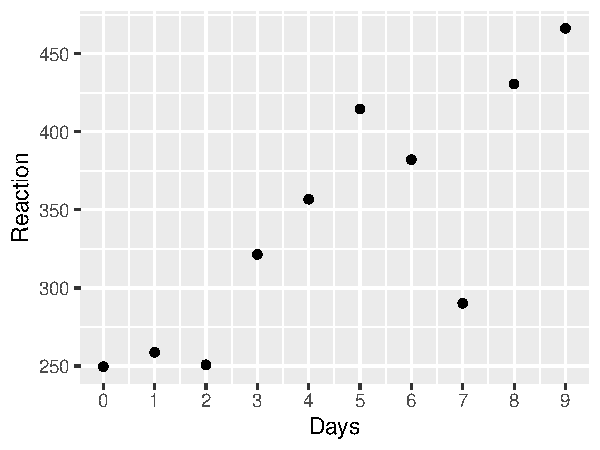
\includegraphics[width=0.5\linewidth]{05-介绍线性混合效应模型_files/figure-latex/one-subject-1} \caption{*Belenky et al.(2003)中单个被试的数据*}\label{fig:one-subject}
\end{figure}

\textbf{练习}

使用\texttt{ggplot}重现下面的图,这包含了所有18个被试。

\begin{figure}
\centering
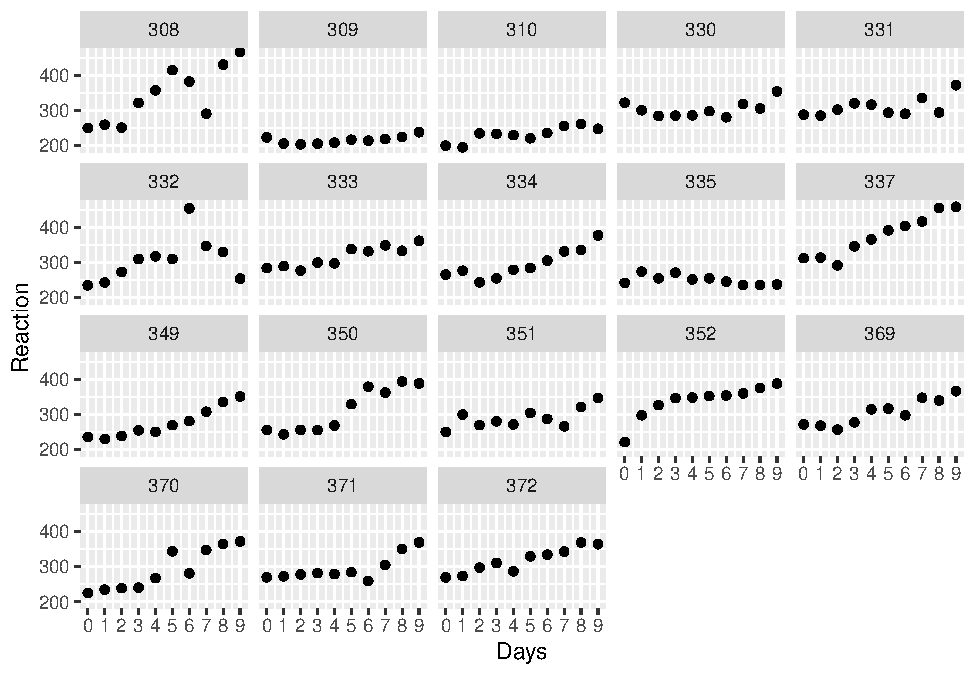
\includegraphics{05-介绍线性混合效应模型_files/figure-latex/plot-solution0-1.pdf}
\caption{\label{fig:plot-solution0}\emph{Belenky et al.(2003)中的数据}}
\end{figure}

从第2天开始到第10天,RT似乎随着睡眠剥夺天数的增加而增加。

请提示

上面给出了绘制单个被试数据的代码。通过去掉\texttt{filter()}语句并添加以\texttt{facet\_}开头的\emph{\texttt{ggplot2}}函数,将此代码改为显示所有被试的数据。

展示答案

和上面一样,只是你要增加一行:\texttt{facet\_wrap(\textasciitilde{}Subject)}

\begin{Shaded}
\begin{Highlighting}[]
\FunctionTok{ggplot}\NormalTok{(sleepstudy, }\FunctionTok{aes}\NormalTok{(}\AttributeTok{x =}\NormalTok{ Days, }\AttributeTok{y =}\NormalTok{ Reaction)) }\SpecialCharTok{+}
  \FunctionTok{geom\_point}\NormalTok{() }\SpecialCharTok{+}
  \FunctionTok{scale\_x\_continuous}\NormalTok{(}\AttributeTok{breaks =} \DecValTok{0}\SpecialCharTok{:}\DecValTok{9}\NormalTok{) }\SpecialCharTok{+}
  \FunctionTok{facet\_wrap}\NormalTok{(}\SpecialCharTok{\textasciitilde{}}\NormalTok{Subject)}
\end{Highlighting}
\end{Shaded}

\hypertarget{ux5982ux4f55ux5bf9ux8fd9ux4e9bux6570ux636eux8fdbux884cux5efaux6a21}{%
\section{如何对这些数据进行建模}\label{ux5982ux4f55ux5bf9ux8fd9ux4e9bux6570ux636eux8fdbux884cux5efaux6a21}}

要合理地对数据进行建模,我们首先需要了解更多关于设计的信息 \citet{Belenky_et_al_2003} 在他们的研究中是这样描述的(p.~2):

\begin{quote}
前3天(T1、T2和B)是适应和训练(T1和T2)以及基线(B),被试要求从23:00到07:00上床睡觉{[}在床时间(time in bed,TIB)为8小时{]}。在第3天(B),进行了基线测量。从第4天开始,连续7天(E1-E7),被试处于4种睡眠条件之一{[}TIB为9小时(22:00--07:00),TIB为7小时(24:00--07:00),TIB为5小时(02:00--07:00)或TIB为3小时(04:00--07:00){]},实际上是一种睡眠延长条件和三种睡眠限制条件。
\end{quote}

从第3天之后的第1晚开始,有7晚的睡眠限制。前2天,编码为\texttt{0}、\texttt{1},是适应(adaptation)和训练(training)。编码为\texttt{2}的那天是进行基线测量的时间,应该是我们分析开始的地方。如果我们将\texttt{0}和\texttt{1}两天包含在我们的分析中,可能会偏倚(bias)我们的结果,因为前两天的任何表现变化都与训练有关,而不是与睡眠限制有关。

\textbf{\emph{练习}}

从数据集中删除\texttt{Days}编码为\texttt{0}或\texttt{1}的观察值,然后根据\texttt{Days}变量创建一个新的变量\texttt{days\_deprived},使序列从第2天开始,第2天重新编码为第0天,第3天为第1天,第4天为第2天,依此类推。这个新变量现在追踪睡眠剥夺的天数。将新表存储为\texttt{sleep2}。

展开答案

\begin{Shaded}
\begin{Highlighting}[]
\NormalTok{sleep2 }\OtherTok{\textless{}{-}}\NormalTok{ sleepstudy }\SpecialCharTok{\%\textgreater{}\%}
  \FunctionTok{filter}\NormalTok{(Days }\SpecialCharTok{\textgreater{}=}\NormalTok{ 2L) }\SpecialCharTok{\%\textgreater{}\%}
  \FunctionTok{mutate}\NormalTok{(}\AttributeTok{days\_deprived =}\NormalTok{ Days }\SpecialCharTok{{-}}\NormalTok{ 2L)}
\end{Highlighting}
\end{Shaded}

仔细检查代码是否按预期工作总是一个好主意。首先,看看它:

\begin{Shaded}
\begin{Highlighting}[]
\FunctionTok{head}\NormalTok{(sleep2)}
\end{Highlighting}
\end{Shaded}

\begin{verbatim}
##   Reaction Days Subject days_deprived
## 1 250.8006    2     308             0
## 2 321.4398    3     308             1
## 3 356.8519    4     308             2
## 4 414.6901    5     308             3
## 5 382.2038    6     308             4
## 6 290.1486    7     308             5
\end{verbatim}

检查\texttt{Days}和\texttt{days\_deprivation}是否匹配。

\begin{Shaded}
\begin{Highlighting}[]
\NormalTok{sleep2 }\SpecialCharTok{\%\textgreater{}\%}
  \FunctionTok{count}\NormalTok{(days\_deprived, Days)}
\end{Highlighting}
\end{Shaded}

\begin{verbatim}
##   days_deprived Days  n
## 1             0    2 18
## 2             1    3 18
## 3             2    4 18
## 4             3    5 18
## 5             4    6 18
## 6             5    7 18
## 7             6    8 18
## 8             7    9 18
\end{verbatim}

看起来很好. 请注意,由\texttt{count()}生成的变量\texttt{n}会告诉你\texttt{Days}和\texttt{days\_deprivation}的每个唯一组合有多少行。在这种情况下有18行,每个被试1行。

现在让我们重新绘制数据,只查看从第0天到第7天的这8个数据点。我们已经从上面的代码中复制了代码,将\texttt{sleepstudy}替换为\texttt{sleep2},并使用\texttt{days\_deprived}作为我们的\texttt{x}变量。

\begin{Shaded}
\begin{Highlighting}[]
\FunctionTok{ggplot}\NormalTok{(sleep2, }\FunctionTok{aes}\NormalTok{(}\AttributeTok{x =}\NormalTok{ days\_deprived, }\AttributeTok{y =}\NormalTok{ Reaction)) }\SpecialCharTok{+}
  \FunctionTok{geom\_point}\NormalTok{() }\SpecialCharTok{+}
  \FunctionTok{scale\_x\_continuous}\NormalTok{(}\AttributeTok{breaks =} \DecValTok{0}\SpecialCharTok{:}\DecValTok{7}\NormalTok{) }\SpecialCharTok{+}
  \FunctionTok{facet\_wrap}\NormalTok{(}\SpecialCharTok{\textasciitilde{}}\NormalTok{Subject) }\SpecialCharTok{+}
  \FunctionTok{labs}\NormalTok{(}\AttributeTok{y =} \StringTok{"反应时"}\NormalTok{, }\AttributeTok{x =} \StringTok{"睡眠剥夺的天数(0 = 基线)"}\NormalTok{)}
\end{Highlighting}
\end{Shaded}

\begin{verbatim}
## Warning in grid.Call(C_textBounds, as.graphicsAnnot(x$label), x$x, x$y, :
## conversion failure on '反应时' in 'mbcsToSbcs': dot substituted for <e5>
\end{verbatim}

\begin{verbatim}
## Warning in grid.Call(C_textBounds, as.graphicsAnnot(x$label), x$x, x$y, :
## conversion failure on '反应时' in 'mbcsToSbcs': dot substituted for <8f>
\end{verbatim}

\begin{verbatim}
## Warning in grid.Call(C_textBounds, as.graphicsAnnot(x$label), x$x, x$y, :
## conversion failure on '反应时' in 'mbcsToSbcs': dot substituted for <8d>
\end{verbatim}

\begin{verbatim}
## Warning in grid.Call(C_textBounds, as.graphicsAnnot(x$label), x$x, x$y, :
## conversion failure on '反应时' in 'mbcsToSbcs': dot substituted for <e5>
\end{verbatim}

\begin{verbatim}
## Warning in grid.Call(C_textBounds, as.graphicsAnnot(x$label), x$x, x$y, :
## conversion failure on '反应时' in 'mbcsToSbcs': dot substituted for <ba>
\end{verbatim}

\begin{verbatim}
## Warning in grid.Call(C_textBounds, as.graphicsAnnot(x$label), x$x, x$y, :
## conversion failure on '反应时' in 'mbcsToSbcs': dot substituted for <94>
\end{verbatim}

\begin{verbatim}
## Warning in grid.Call(C_textBounds, as.graphicsAnnot(x$label), x$x, x$y, :
## conversion failure on '反应时' in 'mbcsToSbcs': dot substituted for <e6>
\end{verbatim}

\begin{verbatim}
## Warning in grid.Call(C_textBounds, as.graphicsAnnot(x$label), x$x, x$y, :
## conversion failure on '反应时' in 'mbcsToSbcs': dot substituted for <97>
\end{verbatim}

\begin{verbatim}
## Warning in grid.Call(C_textBounds, as.graphicsAnnot(x$label), x$x, x$y, :
## conversion failure on '反应时' in 'mbcsToSbcs': dot substituted for <b6>
\end{verbatim}

\begin{verbatim}
## Warning in grid.Call(C_textBounds, as.graphicsAnnot(x$label), x$x, x$y, :
## conversion failure on '睡眠剥夺的天数(0 = 基线)' in 'mbcsToSbcs': dot
## substituted for <e7>
\end{verbatim}

\begin{verbatim}
## Warning in grid.Call(C_textBounds, as.graphicsAnnot(x$label), x$x, x$y, :
## conversion failure on '睡眠剥夺的天数(0 = 基线)' in 'mbcsToSbcs': dot
## substituted for <9d>
\end{verbatim}

\begin{verbatim}
## Warning in grid.Call(C_textBounds, as.graphicsAnnot(x$label), x$x, x$y, :
## conversion failure on '睡眠剥夺的天数(0 = 基线)' in 'mbcsToSbcs': dot
## substituted for <a1>
\end{verbatim}

\begin{verbatim}
## Warning in grid.Call(C_textBounds, as.graphicsAnnot(x$label), x$x, x$y, :
## conversion failure on '睡眠剥夺的天数(0 = 基线)' in 'mbcsToSbcs': dot
## substituted for <e7>
\end{verbatim}

\begin{verbatim}
## Warning in grid.Call(C_textBounds, as.graphicsAnnot(x$label), x$x, x$y, :
## conversion failure on '睡眠剥夺的天数(0 = 基线)' in 'mbcsToSbcs': dot
## substituted for <9c>
\end{verbatim}

\begin{verbatim}
## Warning in grid.Call(C_textBounds, as.graphicsAnnot(x$label), x$x, x$y, :
## conversion failure on '睡眠剥夺的天数(0 = 基线)' in 'mbcsToSbcs': dot
## substituted for <a0>
\end{verbatim}

\begin{verbatim}
## Warning in grid.Call(C_textBounds, as.graphicsAnnot(x$label), x$x, x$y, :
## conversion failure on '睡眠剥夺的天数(0 = 基线)' in 'mbcsToSbcs': dot
## substituted for <e5>
\end{verbatim}

\begin{verbatim}
## Warning in grid.Call(C_textBounds, as.graphicsAnnot(x$label), x$x, x$y, :
## conversion failure on '睡眠剥夺的天数(0 = 基线)' in 'mbcsToSbcs': dot
## substituted for <89>
\end{verbatim}

\begin{verbatim}
## Warning in grid.Call(C_textBounds, as.graphicsAnnot(x$label), x$x, x$y, :
## conversion failure on '睡眠剥夺的天数(0 = 基线)' in 'mbcsToSbcs': dot
## substituted for <a5>
\end{verbatim}

\begin{verbatim}
## Warning in grid.Call(C_textBounds, as.graphicsAnnot(x$label), x$x, x$y, :
## conversion failure on '睡眠剥夺的天数(0 = 基线)' in 'mbcsToSbcs': dot
## substituted for <e5>
\end{verbatim}

\begin{verbatim}
## Warning in grid.Call(C_textBounds, as.graphicsAnnot(x$label), x$x, x$y, :
## conversion failure on '睡眠剥夺的天数(0 = 基线)' in 'mbcsToSbcs': dot
## substituted for <a4>
\end{verbatim}

\begin{verbatim}
## Warning in grid.Call(C_textBounds, as.graphicsAnnot(x$label), x$x, x$y, :
## conversion failure on '睡眠剥夺的天数(0 = 基线)' in 'mbcsToSbcs': dot
## substituted for <ba>
\end{verbatim}

\begin{verbatim}
## Warning in grid.Call(C_textBounds, as.graphicsAnnot(x$label), x$x, x$y, :
## conversion failure on '睡眠剥夺的天数(0 = 基线)' in 'mbcsToSbcs': dot
## substituted for <e7>
\end{verbatim}

\begin{verbatim}
## Warning in grid.Call(C_textBounds, as.graphicsAnnot(x$label), x$x, x$y, :
## conversion failure on '睡眠剥夺的天数(0 = 基线)' in 'mbcsToSbcs': dot
## substituted for <9a>
\end{verbatim}

\begin{verbatim}
## Warning in grid.Call(C_textBounds, as.graphicsAnnot(x$label), x$x, x$y, :
## conversion failure on '睡眠剥夺的天数(0 = 基线)' in 'mbcsToSbcs': dot
## substituted for <84>
\end{verbatim}

\begin{verbatim}
## Warning in grid.Call(C_textBounds, as.graphicsAnnot(x$label), x$x, x$y, :
## conversion failure on '睡眠剥夺的天数(0 = 基线)' in 'mbcsToSbcs': dot
## substituted for <e5>
\end{verbatim}

\begin{verbatim}
## Warning in grid.Call(C_textBounds, as.graphicsAnnot(x$label), x$x, x$y, :
## conversion failure on '睡眠剥夺的天数(0 = 基线)' in 'mbcsToSbcs': dot
## substituted for <a4>
\end{verbatim}

\begin{verbatim}
## Warning in grid.Call(C_textBounds, as.graphicsAnnot(x$label), x$x, x$y, :
## conversion failure on '睡眠剥夺的天数(0 = 基线)' in 'mbcsToSbcs': dot
## substituted for <a9>
\end{verbatim}

\begin{verbatim}
## Warning in grid.Call(C_textBounds, as.graphicsAnnot(x$label), x$x, x$y, :
## conversion failure on '睡眠剥夺的天数(0 = 基线)' in 'mbcsToSbcs': dot
## substituted for <e6>
\end{verbatim}

\begin{verbatim}
## Warning in grid.Call(C_textBounds, as.graphicsAnnot(x$label), x$x, x$y, :
## conversion failure on '睡眠剥夺的天数(0 = 基线)' in 'mbcsToSbcs': dot
## substituted for <95>
\end{verbatim}

\begin{verbatim}
## Warning in grid.Call(C_textBounds, as.graphicsAnnot(x$label), x$x, x$y, :
## conversion failure on '睡眠剥夺的天数(0 = 基线)' in 'mbcsToSbcs': dot
## substituted for <b0>
\end{verbatim}

\begin{verbatim}
## Warning in grid.Call(C_textBounds, as.graphicsAnnot(x$label), x$x, x$y, :
## conversion failure on '睡眠剥夺的天数(0 = 基线)' in 'mbcsToSbcs': dot
## substituted for <e5>
\end{verbatim}

\begin{verbatim}
## Warning in grid.Call(C_textBounds, as.graphicsAnnot(x$label), x$x, x$y, :
## conversion failure on '睡眠剥夺的天数(0 = 基线)' in 'mbcsToSbcs': dot
## substituted for <9f>
\end{verbatim}

\begin{verbatim}
## Warning in grid.Call(C_textBounds, as.graphicsAnnot(x$label), x$x, x$y, :
## conversion failure on '睡眠剥夺的天数(0 = 基线)' in 'mbcsToSbcs': dot
## substituted for <ba>
\end{verbatim}

\begin{verbatim}
## Warning in grid.Call(C_textBounds, as.graphicsAnnot(x$label), x$x, x$y, :
## conversion failure on '睡眠剥夺的天数(0 = 基线)' in 'mbcsToSbcs': dot
## substituted for <e7>
\end{verbatim}

\begin{verbatim}
## Warning in grid.Call(C_textBounds, as.graphicsAnnot(x$label), x$x, x$y, :
## conversion failure on '睡眠剥夺的天数(0 = 基线)' in 'mbcsToSbcs': dot
## substituted for <ba>
\end{verbatim}

\begin{verbatim}
## Warning in grid.Call(C_textBounds, as.graphicsAnnot(x$label), x$x, x$y, :
## conversion failure on '睡眠剥夺的天数(0 = 基线)' in 'mbcsToSbcs': dot
## substituted for <bf>
\end{verbatim}

\begin{verbatim}
## Warning in grid.Call.graphics(C_text, as.graphicsAnnot(x$label), x$x, x$y, :
## conversion failure on '睡眠剥夺的天数(0 = 基线)' in 'mbcsToSbcs': dot
## substituted for <e7>
\end{verbatim}

\begin{verbatim}
## Warning in grid.Call.graphics(C_text, as.graphicsAnnot(x$label), x$x, x$y, :
## conversion failure on '睡眠剥夺的天数(0 = 基线)' in 'mbcsToSbcs': dot
## substituted for <9d>
\end{verbatim}

\begin{verbatim}
## Warning in grid.Call.graphics(C_text, as.graphicsAnnot(x$label), x$x, x$y, :
## conversion failure on '睡眠剥夺的天数(0 = 基线)' in 'mbcsToSbcs': dot
## substituted for <a1>
\end{verbatim}

\begin{verbatim}
## Warning in grid.Call.graphics(C_text, as.graphicsAnnot(x$label), x$x, x$y, :
## conversion failure on '睡眠剥夺的天数(0 = 基线)' in 'mbcsToSbcs': dot
## substituted for <e7>
\end{verbatim}

\begin{verbatim}
## Warning in grid.Call.graphics(C_text, as.graphicsAnnot(x$label), x$x, x$y, :
## conversion failure on '睡眠剥夺的天数(0 = 基线)' in 'mbcsToSbcs': dot
## substituted for <9c>
\end{verbatim}

\begin{verbatim}
## Warning in grid.Call.graphics(C_text, as.graphicsAnnot(x$label), x$x, x$y, :
## conversion failure on '睡眠剥夺的天数(0 = 基线)' in 'mbcsToSbcs': dot
## substituted for <a0>
\end{verbatim}

\begin{verbatim}
## Warning in grid.Call.graphics(C_text, as.graphicsAnnot(x$label), x$x, x$y, :
## conversion failure on '睡眠剥夺的天数(0 = 基线)' in 'mbcsToSbcs': dot
## substituted for <e5>
\end{verbatim}

\begin{verbatim}
## Warning in grid.Call.graphics(C_text, as.graphicsAnnot(x$label), x$x, x$y, :
## conversion failure on '睡眠剥夺的天数(0 = 基线)' in 'mbcsToSbcs': dot
## substituted for <89>
\end{verbatim}

\begin{verbatim}
## Warning in grid.Call.graphics(C_text, as.graphicsAnnot(x$label), x$x, x$y, :
## conversion failure on '睡眠剥夺的天数(0 = 基线)' in 'mbcsToSbcs': dot
## substituted for <a5>
\end{verbatim}

\begin{verbatim}
## Warning in grid.Call.graphics(C_text, as.graphicsAnnot(x$label), x$x, x$y, :
## conversion failure on '睡眠剥夺的天数(0 = 基线)' in 'mbcsToSbcs': dot
## substituted for <e5>
\end{verbatim}

\begin{verbatim}
## Warning in grid.Call.graphics(C_text, as.graphicsAnnot(x$label), x$x, x$y, :
## conversion failure on '睡眠剥夺的天数(0 = 基线)' in 'mbcsToSbcs': dot
## substituted for <a4>
\end{verbatim}

\begin{verbatim}
## Warning in grid.Call.graphics(C_text, as.graphicsAnnot(x$label), x$x, x$y, :
## conversion failure on '睡眠剥夺的天数(0 = 基线)' in 'mbcsToSbcs': dot
## substituted for <ba>
\end{verbatim}

\begin{verbatim}
## Warning in grid.Call.graphics(C_text, as.graphicsAnnot(x$label), x$x, x$y, :
## conversion failure on '睡眠剥夺的天数(0 = 基线)' in 'mbcsToSbcs': dot
## substituted for <e7>
\end{verbatim}

\begin{verbatim}
## Warning in grid.Call.graphics(C_text, as.graphicsAnnot(x$label), x$x, x$y, :
## conversion failure on '睡眠剥夺的天数(0 = 基线)' in 'mbcsToSbcs': dot
## substituted for <9a>
\end{verbatim}

\begin{verbatim}
## Warning in grid.Call.graphics(C_text, as.graphicsAnnot(x$label), x$x, x$y, :
## conversion failure on '睡眠剥夺的天数(0 = 基线)' in 'mbcsToSbcs': dot
## substituted for <84>
\end{verbatim}

\begin{verbatim}
## Warning in grid.Call.graphics(C_text, as.graphicsAnnot(x$label), x$x, x$y, :
## conversion failure on '睡眠剥夺的天数(0 = 基线)' in 'mbcsToSbcs': dot
## substituted for <e5>
\end{verbatim}

\begin{verbatim}
## Warning in grid.Call.graphics(C_text, as.graphicsAnnot(x$label), x$x, x$y, :
## conversion failure on '睡眠剥夺的天数(0 = 基线)' in 'mbcsToSbcs': dot
## substituted for <a4>
\end{verbatim}

\begin{verbatim}
## Warning in grid.Call.graphics(C_text, as.graphicsAnnot(x$label), x$x, x$y, :
## conversion failure on '睡眠剥夺的天数(0 = 基线)' in 'mbcsToSbcs': dot
## substituted for <a9>
\end{verbatim}

\begin{verbatim}
## Warning in grid.Call.graphics(C_text, as.graphicsAnnot(x$label), x$x, x$y, :
## conversion failure on '睡眠剥夺的天数(0 = 基线)' in 'mbcsToSbcs': dot
## substituted for <e6>
\end{verbatim}

\begin{verbatim}
## Warning in grid.Call.graphics(C_text, as.graphicsAnnot(x$label), x$x, x$y, :
## conversion failure on '睡眠剥夺的天数(0 = 基线)' in 'mbcsToSbcs': dot
## substituted for <95>
\end{verbatim}

\begin{verbatim}
## Warning in grid.Call.graphics(C_text, as.graphicsAnnot(x$label), x$x, x$y, :
## conversion failure on '睡眠剥夺的天数(0 = 基线)' in 'mbcsToSbcs': dot
## substituted for <b0>
\end{verbatim}

\begin{verbatim}
## Warning in grid.Call.graphics(C_text, as.graphicsAnnot(x$label), x$x, x$y, :
## conversion failure on '睡眠剥夺的天数(0 = 基线)' in 'mbcsToSbcs': dot
## substituted for <e5>
\end{verbatim}

\begin{verbatim}
## Warning in grid.Call.graphics(C_text, as.graphicsAnnot(x$label), x$x, x$y, :
## conversion failure on '睡眠剥夺的天数(0 = 基线)' in 'mbcsToSbcs': dot
## substituted for <9f>
\end{verbatim}

\begin{verbatim}
## Warning in grid.Call.graphics(C_text, as.graphicsAnnot(x$label), x$x, x$y, :
## conversion failure on '睡眠剥夺的天数(0 = 基线)' in 'mbcsToSbcs': dot
## substituted for <ba>
\end{verbatim}

\begin{verbatim}
## Warning in grid.Call.graphics(C_text, as.graphicsAnnot(x$label), x$x, x$y, :
## conversion failure on '睡眠剥夺的天数(0 = 基线)' in 'mbcsToSbcs': dot
## substituted for <e7>
\end{verbatim}

\begin{verbatim}
## Warning in grid.Call.graphics(C_text, as.graphicsAnnot(x$label), x$x, x$y, :
## conversion failure on '睡眠剥夺的天数(0 = 基线)' in 'mbcsToSbcs': dot
## substituted for <ba>
\end{verbatim}

\begin{verbatim}
## Warning in grid.Call.graphics(C_text, as.graphicsAnnot(x$label), x$x, x$y, :
## conversion failure on '睡眠剥夺的天数(0 = 基线)' in 'mbcsToSbcs': dot
## substituted for <bf>
\end{verbatim}

\begin{verbatim}
## Warning in grid.Call.graphics(C_text, as.graphicsAnnot(x$label), x$x, x$y, :
## conversion failure on '反应时' in 'mbcsToSbcs': dot substituted for <e5>
\end{verbatim}

\begin{verbatim}
## Warning in grid.Call.graphics(C_text, as.graphicsAnnot(x$label), x$x, x$y, :
## conversion failure on '反应时' in 'mbcsToSbcs': dot substituted for <8f>
\end{verbatim}

\begin{verbatim}
## Warning in grid.Call.graphics(C_text, as.graphicsAnnot(x$label), x$x, x$y, :
## conversion failure on '反应时' in 'mbcsToSbcs': dot substituted for <8d>
\end{verbatim}

\begin{verbatim}
## Warning in grid.Call.graphics(C_text, as.graphicsAnnot(x$label), x$x, x$y, :
## conversion failure on '反应时' in 'mbcsToSbcs': dot substituted for <e5>
\end{verbatim}

\begin{verbatim}
## Warning in grid.Call.graphics(C_text, as.graphicsAnnot(x$label), x$x, x$y, :
## conversion failure on '反应时' in 'mbcsToSbcs': dot substituted for <ba>
\end{verbatim}

\begin{verbatim}
## Warning in grid.Call.graphics(C_text, as.graphicsAnnot(x$label), x$x, x$y, :
## conversion failure on '反应时' in 'mbcsToSbcs': dot substituted for <94>
\end{verbatim}

\begin{verbatim}
## Warning in grid.Call.graphics(C_text, as.graphicsAnnot(x$label), x$x, x$y, :
## conversion failure on '反应时' in 'mbcsToSbcs': dot substituted for <e6>
\end{verbatim}

\begin{verbatim}
## Warning in grid.Call.graphics(C_text, as.graphicsAnnot(x$label), x$x, x$y, :
## conversion failure on '反应时' in 'mbcsToSbcs': dot substituted for <97>
\end{verbatim}

\begin{verbatim}
## Warning in grid.Call.graphics(C_text, as.graphicsAnnot(x$label), x$x, x$y, :
## conversion failure on '反应时' in 'mbcsToSbcs': dot substituted for <b6>
\end{verbatim}

\begin{figure}
\centering
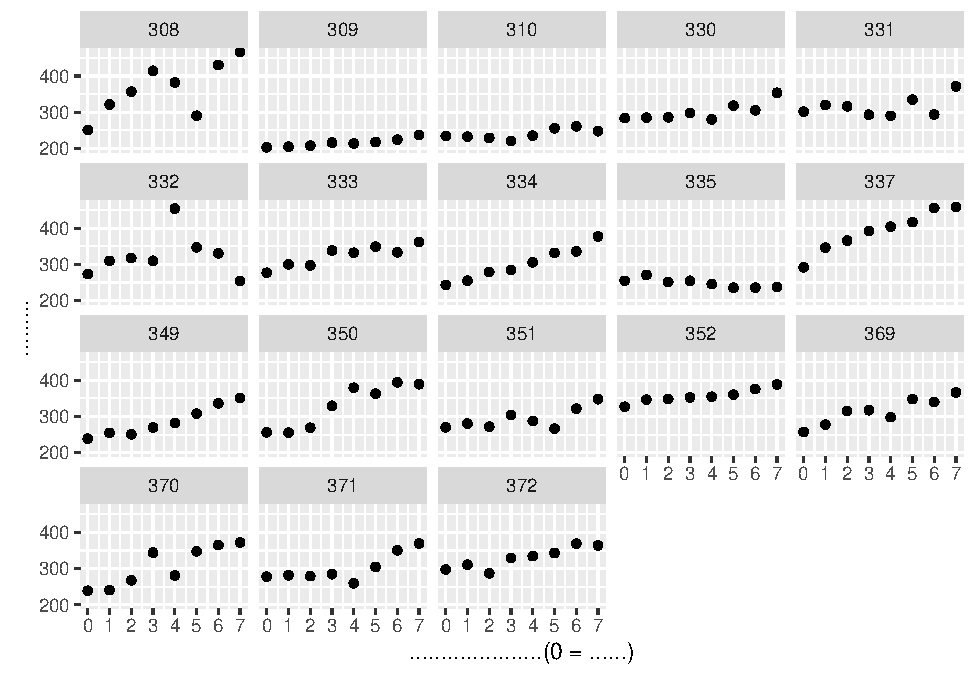
\includegraphics{05-介绍线性混合效应模型_files/figure-latex/plot-solution2-1.pdf}
\caption{\label{fig:plot-solution2}\emph{数据来自Belenky et al.(2003),表示基线(0天)和每天睡眠剥夺后的反应时}}
\end{figure}

请稍作思考,我们如何对\texttt{days\_deprived}和\texttt{Reaction}之间的关系建模。随着睡眠剥夺的增加,反应时间是增加还是减少?这种关系大致稳定还是随时间变化?

除了一个例外(335号被试),看起来反应时随着睡眠剥夺的增加而增加。看起来我们可以对每位被试的数据拟合一条直线。回想一下,一条直线的一般方程形式为\textbf{y = y轴截距 + 斜率 \(\times\) x}。在回归分析中,我们通常用以下公式表示线性关系:

\[Y = \beta_0 + \beta_1 X\]

其中\(\beta_0\)是y轴截距,\(\beta_1\)是斜率,这些参数都是我们从数据中估计而来的。

这些线的截距(剥夺睡眠开始前第0天的平均RT)和斜率(每增加一天的睡眠剥夺后RT的变化)都不同。但我们应该为每个被试拟合同一条线吗?还是每个被试拟合完全不同的线?或者介于两者之间的某种情况?

让我们首先考虑可能用到的三种不同方法。根据McElreath的说法,我们将这些方法称为\textbf{完全混合(complete pooling)}、\textbf{不混合(no pooling)}和\textbf{部分混合(partial pooling)}。

\hypertarget{ux5b8cux5168ux6df7ux5408ux4e00ux5200ux5207}{%
\subsection{完全混合:一刀切}\label{ux5b8cux5168ux6df7ux5408ux4e00ux5200ux5207}}

\textbf{完全混合}是一种``一刀切''模型:它为整个数据集估计单一的截距和斜率,忽略了不同被试在截距或斜率上可能存在的差异。如果这听起来像是一种糟糕的方法,那确实是对的;但你知道这一点是因为你已经可视化了数据,并注意到每个参与者的模式似乎需要不同的y轴截距和斜率值。

拟合出一条线称为``完全混合''方法,因为我们将所有被试的数据混合在一起,得到总体截距和斜率的单一估计。该方法的广义线性模型(GLM)简单地表示为:

\[Y_{sd} = \beta_0 + \beta_1 X_{sd} + e_{sd}\]

\[e_{sd} \sim N\left(0, \sigma^2\right)\]

其中\(Y_{sd}\)是被试\(s\)在第\(d\)天的平均反应时,\(X_{sd}\)是与该情况相关的\texttt{days\_deprived}值(0-7),\(e_{sd}\)是误差。

我们可以在R中用\texttt{lm()}函数拟合一个这样的模型,如下:

\begin{Shaded}
\begin{Highlighting}[]
\NormalTok{cp\_model }\OtherTok{\textless{}{-}} \FunctionTok{lm}\NormalTok{(Reaction }\SpecialCharTok{\textasciitilde{}}\NormalTok{ days\_deprived, sleep2)}

\FunctionTok{summary}\NormalTok{(cp\_model)}
\end{Highlighting}
\end{Shaded}

\begin{verbatim}
## 
## Call:
## lm(formula = Reaction ~ days_deprived, data = sleep2)
## 
## Residuals:
##      Min       1Q   Median       3Q      Max 
## -112.284  -26.732    2.143   27.734  140.453 
## 
## Coefficients:
##               Estimate Std. Error t value Pr(>|t|)    
## (Intercept)    267.967      7.737  34.633  < 2e-16 ***
## days_deprived   11.435      1.850   6.183 6.32e-09 ***
## ---
## Signif. codes:  0 '***' 0.001 '**' 0.01 '*' 0.05 '.' 0.1 ' ' 1
## 
## Residual standard error: 50.85 on 142 degrees of freedom
## Multiple R-squared:  0.2121, Adjusted R-squared:  0.2066 
## F-statistic: 38.23 on 1 and 142 DF,  p-value: 6.316e-09
\end{verbatim}

根据这个模型,第0天的预测平均反应时约为268毫秒,随着剥夺天数的增加,每天的反应时平均增加约11毫秒。然而,我们不能相信回归系数的标准误,因为我们假设所有的观测值都是独立的(严格来说是残差独立)。但我们可以很确定这是一个糟糕的假设。

让我们把模型预测值添加到我们之前创建的图中。我们可以使用\texttt{geom\_abline()}来做到这一点,指定截距和斜率为模型拟合的回归系数\texttt{coef(cp\_model)},该函数返回一个包含截距和斜率两个元素的向量。

\begin{Shaded}
\begin{Highlighting}[]
\FunctionTok{coef}\NormalTok{(cp\_model)}
\end{Highlighting}
\end{Shaded}

\begin{verbatim}
##   (Intercept) days_deprived 
##     267.96742      11.43543
\end{verbatim}

\begin{Shaded}
\begin{Highlighting}[]
\FunctionTok{ggplot}\NormalTok{(sleep2, }\FunctionTok{aes}\NormalTok{(}\AttributeTok{x =}\NormalTok{ days\_deprived, }\AttributeTok{y =}\NormalTok{ Reaction)) }\SpecialCharTok{+}
  \FunctionTok{geom\_abline}\NormalTok{(}\AttributeTok{intercept =} \FunctionTok{coef}\NormalTok{(cp\_model)[}\DecValTok{1}\NormalTok{],}
              \AttributeTok{slope =} \FunctionTok{coef}\NormalTok{(cp\_model)[}\DecValTok{2}\NormalTok{],}
              \AttributeTok{color =} \StringTok{\textquotesingle{}blue\textquotesingle{}}\NormalTok{) }\SpecialCharTok{+}
  \FunctionTok{geom\_point}\NormalTok{() }\SpecialCharTok{+}
  \FunctionTok{scale\_x\_continuous}\NormalTok{(}\AttributeTok{breaks =} \DecValTok{0}\SpecialCharTok{:}\DecValTok{7}\NormalTok{) }\SpecialCharTok{+}
  \FunctionTok{facet\_wrap}\NormalTok{(}\SpecialCharTok{\textasciitilde{}}\NormalTok{Subject) }\SpecialCharTok{+}
  \FunctionTok{labs}\NormalTok{(}\AttributeTok{y =} \StringTok{"反应时"}\NormalTok{, }\AttributeTok{x =} \StringTok{"睡眠剥夺的天数(0 = 基线)"}\NormalTok{)}
\end{Highlighting}
\end{Shaded}

\begin{verbatim}
## Warning in grid.Call(C_textBounds, as.graphicsAnnot(x$label), x$x, x$y, :
## conversion failure on '反应时' in 'mbcsToSbcs': dot substituted for <e5>
\end{verbatim}

\begin{verbatim}
## Warning in grid.Call(C_textBounds, as.graphicsAnnot(x$label), x$x, x$y, :
## conversion failure on '反应时' in 'mbcsToSbcs': dot substituted for <8f>
\end{verbatim}

\begin{verbatim}
## Warning in grid.Call(C_textBounds, as.graphicsAnnot(x$label), x$x, x$y, :
## conversion failure on '反应时' in 'mbcsToSbcs': dot substituted for <8d>
\end{verbatim}

\begin{verbatim}
## Warning in grid.Call(C_textBounds, as.graphicsAnnot(x$label), x$x, x$y, :
## conversion failure on '反应时' in 'mbcsToSbcs': dot substituted for <e5>
\end{verbatim}

\begin{verbatim}
## Warning in grid.Call(C_textBounds, as.graphicsAnnot(x$label), x$x, x$y, :
## conversion failure on '反应时' in 'mbcsToSbcs': dot substituted for <ba>
\end{verbatim}

\begin{verbatim}
## Warning in grid.Call(C_textBounds, as.graphicsAnnot(x$label), x$x, x$y, :
## conversion failure on '反应时' in 'mbcsToSbcs': dot substituted for <94>
\end{verbatim}

\begin{verbatim}
## Warning in grid.Call(C_textBounds, as.graphicsAnnot(x$label), x$x, x$y, :
## conversion failure on '反应时' in 'mbcsToSbcs': dot substituted for <e6>
\end{verbatim}

\begin{verbatim}
## Warning in grid.Call(C_textBounds, as.graphicsAnnot(x$label), x$x, x$y, :
## conversion failure on '反应时' in 'mbcsToSbcs': dot substituted for <97>
\end{verbatim}

\begin{verbatim}
## Warning in grid.Call(C_textBounds, as.graphicsAnnot(x$label), x$x, x$y, :
## conversion failure on '反应时' in 'mbcsToSbcs': dot substituted for <b6>
\end{verbatim}

\begin{verbatim}
## Warning in grid.Call(C_textBounds, as.graphicsAnnot(x$label), x$x, x$y, :
## conversion failure on '睡眠剥夺的天数(0 = 基线)' in 'mbcsToSbcs': dot
## substituted for <e7>
\end{verbatim}

\begin{verbatim}
## Warning in grid.Call(C_textBounds, as.graphicsAnnot(x$label), x$x, x$y, :
## conversion failure on '睡眠剥夺的天数(0 = 基线)' in 'mbcsToSbcs': dot
## substituted for <9d>
\end{verbatim}

\begin{verbatim}
## Warning in grid.Call(C_textBounds, as.graphicsAnnot(x$label), x$x, x$y, :
## conversion failure on '睡眠剥夺的天数(0 = 基线)' in 'mbcsToSbcs': dot
## substituted for <a1>
\end{verbatim}

\begin{verbatim}
## Warning in grid.Call(C_textBounds, as.graphicsAnnot(x$label), x$x, x$y, :
## conversion failure on '睡眠剥夺的天数(0 = 基线)' in 'mbcsToSbcs': dot
## substituted for <e7>
\end{verbatim}

\begin{verbatim}
## Warning in grid.Call(C_textBounds, as.graphicsAnnot(x$label), x$x, x$y, :
## conversion failure on '睡眠剥夺的天数(0 = 基线)' in 'mbcsToSbcs': dot
## substituted for <9c>
\end{verbatim}

\begin{verbatim}
## Warning in grid.Call(C_textBounds, as.graphicsAnnot(x$label), x$x, x$y, :
## conversion failure on '睡眠剥夺的天数(0 = 基线)' in 'mbcsToSbcs': dot
## substituted for <a0>
\end{verbatim}

\begin{verbatim}
## Warning in grid.Call(C_textBounds, as.graphicsAnnot(x$label), x$x, x$y, :
## conversion failure on '睡眠剥夺的天数(0 = 基线)' in 'mbcsToSbcs': dot
## substituted for <e5>
\end{verbatim}

\begin{verbatim}
## Warning in grid.Call(C_textBounds, as.graphicsAnnot(x$label), x$x, x$y, :
## conversion failure on '睡眠剥夺的天数(0 = 基线)' in 'mbcsToSbcs': dot
## substituted for <89>
\end{verbatim}

\begin{verbatim}
## Warning in grid.Call(C_textBounds, as.graphicsAnnot(x$label), x$x, x$y, :
## conversion failure on '睡眠剥夺的天数(0 = 基线)' in 'mbcsToSbcs': dot
## substituted for <a5>
\end{verbatim}

\begin{verbatim}
## Warning in grid.Call(C_textBounds, as.graphicsAnnot(x$label), x$x, x$y, :
## conversion failure on '睡眠剥夺的天数(0 = 基线)' in 'mbcsToSbcs': dot
## substituted for <e5>
\end{verbatim}

\begin{verbatim}
## Warning in grid.Call(C_textBounds, as.graphicsAnnot(x$label), x$x, x$y, :
## conversion failure on '睡眠剥夺的天数(0 = 基线)' in 'mbcsToSbcs': dot
## substituted for <a4>
\end{verbatim}

\begin{verbatim}
## Warning in grid.Call(C_textBounds, as.graphicsAnnot(x$label), x$x, x$y, :
## conversion failure on '睡眠剥夺的天数(0 = 基线)' in 'mbcsToSbcs': dot
## substituted for <ba>
\end{verbatim}

\begin{verbatim}
## Warning in grid.Call(C_textBounds, as.graphicsAnnot(x$label), x$x, x$y, :
## conversion failure on '睡眠剥夺的天数(0 = 基线)' in 'mbcsToSbcs': dot
## substituted for <e7>
\end{verbatim}

\begin{verbatim}
## Warning in grid.Call(C_textBounds, as.graphicsAnnot(x$label), x$x, x$y, :
## conversion failure on '睡眠剥夺的天数(0 = 基线)' in 'mbcsToSbcs': dot
## substituted for <9a>
\end{verbatim}

\begin{verbatim}
## Warning in grid.Call(C_textBounds, as.graphicsAnnot(x$label), x$x, x$y, :
## conversion failure on '睡眠剥夺的天数(0 = 基线)' in 'mbcsToSbcs': dot
## substituted for <84>
\end{verbatim}

\begin{verbatim}
## Warning in grid.Call(C_textBounds, as.graphicsAnnot(x$label), x$x, x$y, :
## conversion failure on '睡眠剥夺的天数(0 = 基线)' in 'mbcsToSbcs': dot
## substituted for <e5>
\end{verbatim}

\begin{verbatim}
## Warning in grid.Call(C_textBounds, as.graphicsAnnot(x$label), x$x, x$y, :
## conversion failure on '睡眠剥夺的天数(0 = 基线)' in 'mbcsToSbcs': dot
## substituted for <a4>
\end{verbatim}

\begin{verbatim}
## Warning in grid.Call(C_textBounds, as.graphicsAnnot(x$label), x$x, x$y, :
## conversion failure on '睡眠剥夺的天数(0 = 基线)' in 'mbcsToSbcs': dot
## substituted for <a9>
\end{verbatim}

\begin{verbatim}
## Warning in grid.Call(C_textBounds, as.graphicsAnnot(x$label), x$x, x$y, :
## conversion failure on '睡眠剥夺的天数(0 = 基线)' in 'mbcsToSbcs': dot
## substituted for <e6>
\end{verbatim}

\begin{verbatim}
## Warning in grid.Call(C_textBounds, as.graphicsAnnot(x$label), x$x, x$y, :
## conversion failure on '睡眠剥夺的天数(0 = 基线)' in 'mbcsToSbcs': dot
## substituted for <95>
\end{verbatim}

\begin{verbatim}
## Warning in grid.Call(C_textBounds, as.graphicsAnnot(x$label), x$x, x$y, :
## conversion failure on '睡眠剥夺的天数(0 = 基线)' in 'mbcsToSbcs': dot
## substituted for <b0>
\end{verbatim}

\begin{verbatim}
## Warning in grid.Call(C_textBounds, as.graphicsAnnot(x$label), x$x, x$y, :
## conversion failure on '睡眠剥夺的天数(0 = 基线)' in 'mbcsToSbcs': dot
## substituted for <e5>
\end{verbatim}

\begin{verbatim}
## Warning in grid.Call(C_textBounds, as.graphicsAnnot(x$label), x$x, x$y, :
## conversion failure on '睡眠剥夺的天数(0 = 基线)' in 'mbcsToSbcs': dot
## substituted for <9f>
\end{verbatim}

\begin{verbatim}
## Warning in grid.Call(C_textBounds, as.graphicsAnnot(x$label), x$x, x$y, :
## conversion failure on '睡眠剥夺的天数(0 = 基线)' in 'mbcsToSbcs': dot
## substituted for <ba>
\end{verbatim}

\begin{verbatim}
## Warning in grid.Call(C_textBounds, as.graphicsAnnot(x$label), x$x, x$y, :
## conversion failure on '睡眠剥夺的天数(0 = 基线)' in 'mbcsToSbcs': dot
## substituted for <e7>
\end{verbatim}

\begin{verbatim}
## Warning in grid.Call(C_textBounds, as.graphicsAnnot(x$label), x$x, x$y, :
## conversion failure on '睡眠剥夺的天数(0 = 基线)' in 'mbcsToSbcs': dot
## substituted for <ba>
\end{verbatim}

\begin{verbatim}
## Warning in grid.Call(C_textBounds, as.graphicsAnnot(x$label), x$x, x$y, :
## conversion failure on '睡眠剥夺的天数(0 = 基线)' in 'mbcsToSbcs': dot
## substituted for <bf>
\end{verbatim}

\begin{verbatim}
## Warning in grid.Call.graphics(C_text, as.graphicsAnnot(x$label), x$x, x$y, :
## conversion failure on '睡眠剥夺的天数(0 = 基线)' in 'mbcsToSbcs': dot
## substituted for <e7>
\end{verbatim}

\begin{verbatim}
## Warning in grid.Call.graphics(C_text, as.graphicsAnnot(x$label), x$x, x$y, :
## conversion failure on '睡眠剥夺的天数(0 = 基线)' in 'mbcsToSbcs': dot
## substituted for <9d>
\end{verbatim}

\begin{verbatim}
## Warning in grid.Call.graphics(C_text, as.graphicsAnnot(x$label), x$x, x$y, :
## conversion failure on '睡眠剥夺的天数(0 = 基线)' in 'mbcsToSbcs': dot
## substituted for <a1>
\end{verbatim}

\begin{verbatim}
## Warning in grid.Call.graphics(C_text, as.graphicsAnnot(x$label), x$x, x$y, :
## conversion failure on '睡眠剥夺的天数(0 = 基线)' in 'mbcsToSbcs': dot
## substituted for <e7>
\end{verbatim}

\begin{verbatim}
## Warning in grid.Call.graphics(C_text, as.graphicsAnnot(x$label), x$x, x$y, :
## conversion failure on '睡眠剥夺的天数(0 = 基线)' in 'mbcsToSbcs': dot
## substituted for <9c>
\end{verbatim}

\begin{verbatim}
## Warning in grid.Call.graphics(C_text, as.graphicsAnnot(x$label), x$x, x$y, :
## conversion failure on '睡眠剥夺的天数(0 = 基线)' in 'mbcsToSbcs': dot
## substituted for <a0>
\end{verbatim}

\begin{verbatim}
## Warning in grid.Call.graphics(C_text, as.graphicsAnnot(x$label), x$x, x$y, :
## conversion failure on '睡眠剥夺的天数(0 = 基线)' in 'mbcsToSbcs': dot
## substituted for <e5>
\end{verbatim}

\begin{verbatim}
## Warning in grid.Call.graphics(C_text, as.graphicsAnnot(x$label), x$x, x$y, :
## conversion failure on '睡眠剥夺的天数(0 = 基线)' in 'mbcsToSbcs': dot
## substituted for <89>
\end{verbatim}

\begin{verbatim}
## Warning in grid.Call.graphics(C_text, as.graphicsAnnot(x$label), x$x, x$y, :
## conversion failure on '睡眠剥夺的天数(0 = 基线)' in 'mbcsToSbcs': dot
## substituted for <a5>
\end{verbatim}

\begin{verbatim}
## Warning in grid.Call.graphics(C_text, as.graphicsAnnot(x$label), x$x, x$y, :
## conversion failure on '睡眠剥夺的天数(0 = 基线)' in 'mbcsToSbcs': dot
## substituted for <e5>
\end{verbatim}

\begin{verbatim}
## Warning in grid.Call.graphics(C_text, as.graphicsAnnot(x$label), x$x, x$y, :
## conversion failure on '睡眠剥夺的天数(0 = 基线)' in 'mbcsToSbcs': dot
## substituted for <a4>
\end{verbatim}

\begin{verbatim}
## Warning in grid.Call.graphics(C_text, as.graphicsAnnot(x$label), x$x, x$y, :
## conversion failure on '睡眠剥夺的天数(0 = 基线)' in 'mbcsToSbcs': dot
## substituted for <ba>
\end{verbatim}

\begin{verbatim}
## Warning in grid.Call.graphics(C_text, as.graphicsAnnot(x$label), x$x, x$y, :
## conversion failure on '睡眠剥夺的天数(0 = 基线)' in 'mbcsToSbcs': dot
## substituted for <e7>
\end{verbatim}

\begin{verbatim}
## Warning in grid.Call.graphics(C_text, as.graphicsAnnot(x$label), x$x, x$y, :
## conversion failure on '睡眠剥夺的天数(0 = 基线)' in 'mbcsToSbcs': dot
## substituted for <9a>
\end{verbatim}

\begin{verbatim}
## Warning in grid.Call.graphics(C_text, as.graphicsAnnot(x$label), x$x, x$y, :
## conversion failure on '睡眠剥夺的天数(0 = 基线)' in 'mbcsToSbcs': dot
## substituted for <84>
\end{verbatim}

\begin{verbatim}
## Warning in grid.Call.graphics(C_text, as.graphicsAnnot(x$label), x$x, x$y, :
## conversion failure on '睡眠剥夺的天数(0 = 基线)' in 'mbcsToSbcs': dot
## substituted for <e5>
\end{verbatim}

\begin{verbatim}
## Warning in grid.Call.graphics(C_text, as.graphicsAnnot(x$label), x$x, x$y, :
## conversion failure on '睡眠剥夺的天数(0 = 基线)' in 'mbcsToSbcs': dot
## substituted for <a4>
\end{verbatim}

\begin{verbatim}
## Warning in grid.Call.graphics(C_text, as.graphicsAnnot(x$label), x$x, x$y, :
## conversion failure on '睡眠剥夺的天数(0 = 基线)' in 'mbcsToSbcs': dot
## substituted for <a9>
\end{verbatim}

\begin{verbatim}
## Warning in grid.Call.graphics(C_text, as.graphicsAnnot(x$label), x$x, x$y, :
## conversion failure on '睡眠剥夺的天数(0 = 基线)' in 'mbcsToSbcs': dot
## substituted for <e6>
\end{verbatim}

\begin{verbatim}
## Warning in grid.Call.graphics(C_text, as.graphicsAnnot(x$label), x$x, x$y, :
## conversion failure on '睡眠剥夺的天数(0 = 基线)' in 'mbcsToSbcs': dot
## substituted for <95>
\end{verbatim}

\begin{verbatim}
## Warning in grid.Call.graphics(C_text, as.graphicsAnnot(x$label), x$x, x$y, :
## conversion failure on '睡眠剥夺的天数(0 = 基线)' in 'mbcsToSbcs': dot
## substituted for <b0>
\end{verbatim}

\begin{verbatim}
## Warning in grid.Call.graphics(C_text, as.graphicsAnnot(x$label), x$x, x$y, :
## conversion failure on '睡眠剥夺的天数(0 = 基线)' in 'mbcsToSbcs': dot
## substituted for <e5>
\end{verbatim}

\begin{verbatim}
## Warning in grid.Call.graphics(C_text, as.graphicsAnnot(x$label), x$x, x$y, :
## conversion failure on '睡眠剥夺的天数(0 = 基线)' in 'mbcsToSbcs': dot
## substituted for <9f>
\end{verbatim}

\begin{verbatim}
## Warning in grid.Call.graphics(C_text, as.graphicsAnnot(x$label), x$x, x$y, :
## conversion failure on '睡眠剥夺的天数(0 = 基线)' in 'mbcsToSbcs': dot
## substituted for <ba>
\end{verbatim}

\begin{verbatim}
## Warning in grid.Call.graphics(C_text, as.graphicsAnnot(x$label), x$x, x$y, :
## conversion failure on '睡眠剥夺的天数(0 = 基线)' in 'mbcsToSbcs': dot
## substituted for <e7>
\end{verbatim}

\begin{verbatim}
## Warning in grid.Call.graphics(C_text, as.graphicsAnnot(x$label), x$x, x$y, :
## conversion failure on '睡眠剥夺的天数(0 = 基线)' in 'mbcsToSbcs': dot
## substituted for <ba>
\end{verbatim}

\begin{verbatim}
## Warning in grid.Call.graphics(C_text, as.graphicsAnnot(x$label), x$x, x$y, :
## conversion failure on '睡眠剥夺的天数(0 = 基线)' in 'mbcsToSbcs': dot
## substituted for <bf>
\end{verbatim}

\begin{verbatim}
## Warning in grid.Call.graphics(C_text, as.graphicsAnnot(x$label), x$x, x$y, :
## conversion failure on '反应时' in 'mbcsToSbcs': dot substituted for <e5>
\end{verbatim}

\begin{verbatim}
## Warning in grid.Call.graphics(C_text, as.graphicsAnnot(x$label), x$x, x$y, :
## conversion failure on '反应时' in 'mbcsToSbcs': dot substituted for <8f>
\end{verbatim}

\begin{verbatim}
## Warning in grid.Call.graphics(C_text, as.graphicsAnnot(x$label), x$x, x$y, :
## conversion failure on '反应时' in 'mbcsToSbcs': dot substituted for <8d>
\end{verbatim}

\begin{verbatim}
## Warning in grid.Call.graphics(C_text, as.graphicsAnnot(x$label), x$x, x$y, :
## conversion failure on '反应时' in 'mbcsToSbcs': dot substituted for <e5>
\end{verbatim}

\begin{verbatim}
## Warning in grid.Call.graphics(C_text, as.graphicsAnnot(x$label), x$x, x$y, :
## conversion failure on '反应时' in 'mbcsToSbcs': dot substituted for <ba>
\end{verbatim}

\begin{verbatim}
## Warning in grid.Call.graphics(C_text, as.graphicsAnnot(x$label), x$x, x$y, :
## conversion failure on '反应时' in 'mbcsToSbcs': dot substituted for <94>
\end{verbatim}

\begin{verbatim}
## Warning in grid.Call.graphics(C_text, as.graphicsAnnot(x$label), x$x, x$y, :
## conversion failure on '反应时' in 'mbcsToSbcs': dot substituted for <e6>
\end{verbatim}

\begin{verbatim}
## Warning in grid.Call.graphics(C_text, as.graphicsAnnot(x$label), x$x, x$y, :
## conversion failure on '反应时' in 'mbcsToSbcs': dot substituted for <97>
\end{verbatim}

\begin{verbatim}
## Warning in grid.Call.graphics(C_text, as.graphicsAnnot(x$label), x$x, x$y, :
## conversion failure on '反应时' in 'mbcsToSbcs': dot substituted for <b6>
\end{verbatim}

\begin{figure}
\centering
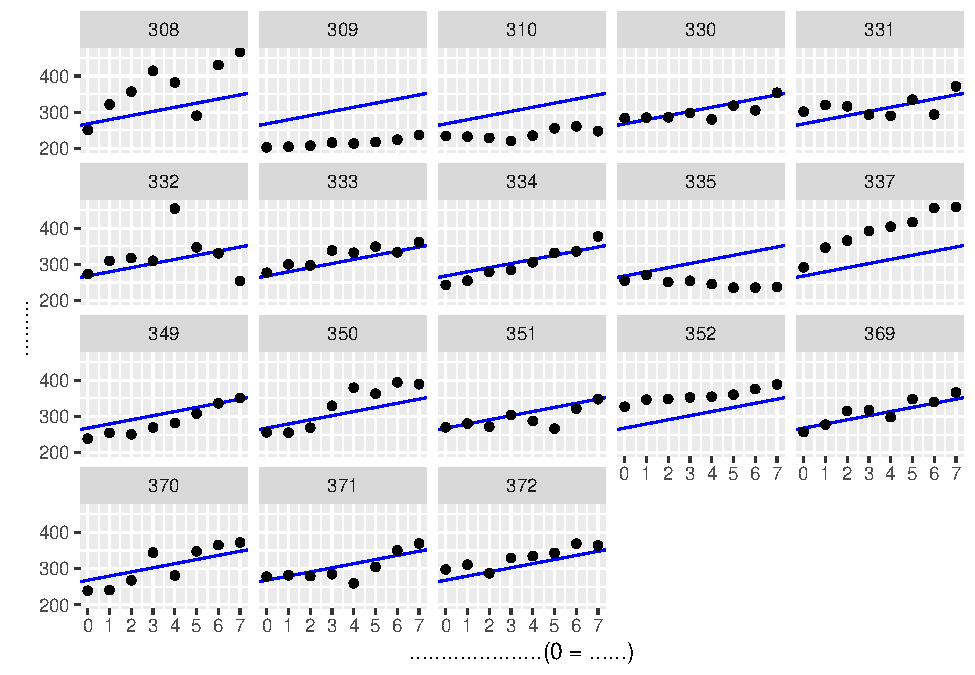
\includegraphics{05-介绍线性混合效应模型_files/figure-latex/cp-model-plot-1.pdf}
\caption{\label{fig:cp-model-plot}原始数据和完全混合模型的拟合结果对比图}
\end{figure}

这个模型与数据不太吻合。我们需要一种不同的方法。

\hypertarget{ux4e0dux6df7ux5408}{%
\subsection{不混合}\label{ux4e0dux6df7ux5408}}

将所有信息混合成一个截距和一个斜率来估计是不合适的。另一种方法是为每个被试拟合单独的线。这意味着每个被试的估计值将完全不受其他被试估计值的影响。换句话说,我们可以分别估计18组单独的截距/斜率对。

这个模型可以通过两种方式实现:(1)为每个被试运行单独的回归或(2)运行混合效应回归。我们将采用后者,这样所有内容都在一个大模型中。我们已经知道了如何做到这一点:我们为\texttt{Subject}因子添加虚拟编码。这个因子有18个水平,所以我们需要17个虚拟编码。幸运的是,R为我们省去了手动创建这17个变量的麻烦。我们只需要在模型中纳入\texttt{Subject}作为预测变量,并将这个分类预测变量与\texttt{days\_deprived}进行交互,以允许截距和斜率变化。

\texttt{sleep2}数据集中的变量\texttt{Subject}是名义变量。我们只是用数字作为标签来保证匿名性,并不意味着被试310比被试309好1点,或者比被试308好2点。确保将其定义为因子变量,而不是作为连续变量包含在内!

我们可以通过多种方式测试某个变量是否为因子变量。其中一种方法是对表格使用\texttt{summary()}函数。

\begin{Shaded}
\begin{Highlighting}[]
\NormalTok{sleep2 }\SpecialCharTok{\%\textgreater{}\%} \FunctionTok{summary}\NormalTok{()}
\end{Highlighting}
\end{Shaded}

\begin{verbatim}
##     Reaction          Days         Subject   days_deprived 
##  Min.   :203.0   Min.   :2.00   308    : 8   Min.   :0.00  
##  1st Qu.:265.2   1st Qu.:3.75   309    : 8   1st Qu.:1.75  
##  Median :303.2   Median :5.50   310    : 8   Median :3.50  
##  Mean   :308.0   Mean   :5.50   330    : 8   Mean   :3.50  
##  3rd Qu.:347.7   3rd Qu.:7.25   331    : 8   3rd Qu.:5.25  
##  Max.   :466.4   Max.   :9.00   332    : 8   Max.   :7.00  
##                                 (Other):96
\end{verbatim}

这里你可以看到它并没有被当做一个数字变量,因为它没给出分布信息(均值等),而是告诉你在每个水平上有多少个观测值。

你也可以直接测试它:

\begin{Shaded}
\begin{Highlighting}[]
\NormalTok{sleep2 }\SpecialCharTok{\%\textgreater{}\%} \FunctionTok{pull}\NormalTok{(Subject) }\SpecialCharTok{\%\textgreater{}\%} \FunctionTok{is.factor}\NormalTok{()}
\end{Highlighting}
\end{Shaded}

\begin{verbatim}
## [1] TRUE
\end{verbatim}

如果某些变量不是因子变量,你可以使用\texttt{factor()}函数重新定义它,使其变为因子变量。

\begin{Shaded}
\begin{Highlighting}[]
\NormalTok{np\_model }\OtherTok{\textless{}{-}} \FunctionTok{lm}\NormalTok{(Reaction }\SpecialCharTok{\textasciitilde{}}\NormalTok{ days\_deprived }\SpecialCharTok{+}\NormalTok{ Subject }\SpecialCharTok{+}\NormalTok{ days\_deprived}\SpecialCharTok{:}\NormalTok{Subject,}
               \AttributeTok{data =}\NormalTok{ sleep2)}

\FunctionTok{summary}\NormalTok{(np\_model)}
\end{Highlighting}
\end{Shaded}

\begin{verbatim}
## 
## Call:
## lm(formula = Reaction ~ days_deprived + Subject + days_deprived:Subject, 
##     data = sleep2)
## 
## Residuals:
##      Min       1Q   Median       3Q      Max 
## -106.521   -8.541    1.143    8.889  128.545 
## 
## Coefficients:
##                          Estimate Std. Error t value Pr(>|t|)    
## (Intercept)              288.2175    16.4772  17.492  < 2e-16 ***
## days_deprived             21.6905     3.9388   5.507 2.49e-07 ***
## Subject309               -87.9262    23.3023  -3.773 0.000264 ***
## Subject310               -62.2856    23.3023  -2.673 0.008685 ** 
## Subject330               -14.9533    23.3023  -0.642 0.522422    
## Subject331                 9.9658    23.3023   0.428 0.669740    
## Subject332                27.8157    23.3023   1.194 0.235215    
## Subject333                -2.7581    23.3023  -0.118 0.906000    
## Subject334               -50.2051    23.3023  -2.155 0.033422 *  
## Subject335               -25.3429    23.3023  -1.088 0.279207    
## Subject337                24.6143    23.3023   1.056 0.293187    
## Subject349               -59.2183    23.3023  -2.541 0.012464 *  
## Subject350               -40.2023    23.3023  -1.725 0.087343 .  
## Subject351               -24.2467    23.3023  -1.041 0.300419    
## Subject352                43.0655    23.3023   1.848 0.067321 .  
## Subject369               -21.5040    23.3023  -0.923 0.358154    
## Subject370               -53.3072    23.3023  -2.288 0.024107 *  
## Subject371               -30.4896    23.3023  -1.308 0.193504    
## Subject372                 2.4772    23.3023   0.106 0.915535    
## days_deprived:Subject309 -17.3334     5.5703  -3.112 0.002380 ** 
## days_deprived:Subject310 -17.7915     5.5703  -3.194 0.001839 ** 
## days_deprived:Subject330 -13.6849     5.5703  -2.457 0.015613 *  
## days_deprived:Subject331 -16.8231     5.5703  -3.020 0.003154 ** 
## days_deprived:Subject332 -19.2947     5.5703  -3.464 0.000765 ***
## days_deprived:Subject333 -10.8151     5.5703  -1.942 0.054796 .  
## days_deprived:Subject334  -3.5745     5.5703  -0.642 0.522423    
## days_deprived:Subject335 -25.8995     5.5703  -4.650 9.47e-06 ***
## days_deprived:Subject337   0.7518     5.5703   0.135 0.892895    
## days_deprived:Subject349  -5.2644     5.5703  -0.945 0.346731    
## days_deprived:Subject350   1.6007     5.5703   0.287 0.774382    
## days_deprived:Subject351 -13.1681     5.5703  -2.364 0.019867 *  
## days_deprived:Subject352 -14.4019     5.5703  -2.585 0.011057 *  
## days_deprived:Subject369  -7.8948     5.5703  -1.417 0.159273    
## days_deprived:Subject370  -1.0495     5.5703  -0.188 0.850912    
## days_deprived:Subject371  -9.3443     5.5703  -1.678 0.096334 .  
## days_deprived:Subject372 -10.6041     5.5703  -1.904 0.059613 .  
## ---
## Signif. codes:  0 '***' 0.001 '**' 0.01 '*' 0.05 '.' 0.1 ' ' 1
## 
## Residual standard error: 25.53 on 108 degrees of freedom
## Multiple R-squared:  0.849,  Adjusted R-squared:  0.8001 
## F-statistic: 17.35 on 35 and 108 DF,  p-value: < 2.2e-16
\end{verbatim}

这个模型将一个被试(具体来说是被试308)作为基线,并通过偏移量来表示每个被试相对于该基线的差异。在我们之前讨论\protect\hyperlink{cont-by-cat}{连续变量-分类变量交互效应}时你已经看过这种方法了。

回答这些问题(结果保留三位小数)

\begin{itemize}
\tightlist
\item
  被试308的截距是多少?\_\_\_\_\_\_\_\_
\item
  被试308的斜率是多少?\_\_\_\_\_\_\_\_
\item
  被试335的截距是多少?\_\_\_\_\_\_\_\_
\item
  被试335的斜率是多少?\_\_\_\_\_\_\_\_
\end{itemize}

答案和解析

基线被试是308------R中默认按字母顺序排列因子的水平,并选择第一个作为基线。这意味着对于被试308,截距由\texttt{(Intercept)}给出,而斜率由\texttt{days\_deprived}给出,因为其他17个虚拟变量对被试308而言都是0。

所有其他被试的回归系数都表示为相对于此基线被试的\emph{偏移量}。如果我们想计算特定受试者的截距和斜率,只需加上相应的偏移量即可。因此,答案如下:

\begin{itemize}
\item
  被试308的截距: 288.217
\item
  被试308的斜率: 21.69
\item
  被试355的截距: \texttt{(Intercept)} + \texttt{Subject335} = 288.217 + -25.343 = 262.874
\item
  被试355的斜率: \texttt{days\_deprived} + \texttt{days\_deprived:Subject335} = 21.69 + -25.899 = -4.209
\end{itemize}

在``不混合''模型中,没有\emph{整个}总体截距和斜率的估计;在这种情况下,\texttt{(Intercept)}和\texttt{days\_deprived}是被试308的截距和斜率的估计,因为被试308被(随意地)选择为基线被试。为了得到总体的估计值,我们可以引入第二阶段分析,计算各个被试的截距和斜率的平均值。让我们使用模型估计值来计算每个被试的截距和斜率。

\begin{Shaded}
\begin{Highlighting}[]
\NormalTok{all\_intercepts }\OtherTok{\textless{}{-}} \FunctionTok{c}\NormalTok{(}\FunctionTok{coef}\NormalTok{(np\_model)[}\StringTok{"(Intercept)"}\NormalTok{],}
                    \FunctionTok{coef}\NormalTok{(np\_model)[}\DecValTok{3}\SpecialCharTok{:}\DecValTok{19}\NormalTok{] }\SpecialCharTok{+} \FunctionTok{coef}\NormalTok{(np\_model)[}\StringTok{"(Intercept)"}\NormalTok{])}

\NormalTok{all\_slopes  }\OtherTok{\textless{}{-}} \FunctionTok{c}\NormalTok{(}\FunctionTok{coef}\NormalTok{(np\_model)[}\StringTok{"days\_deprived"}\NormalTok{],}
                 \FunctionTok{coef}\NormalTok{(np\_model)[}\DecValTok{20}\SpecialCharTok{:}\DecValTok{36}\NormalTok{] }\SpecialCharTok{+} \FunctionTok{coef}\NormalTok{(np\_model)[}\StringTok{"days\_deprived"}\NormalTok{])}

\NormalTok{ids }\OtherTok{\textless{}{-}}\NormalTok{ sleep2 }\SpecialCharTok{\%\textgreater{}\%} \FunctionTok{pull}\NormalTok{(Subject) }\SpecialCharTok{\%\textgreater{}\%} \FunctionTok{levels}\NormalTok{() }\SpecialCharTok{\%\textgreater{}\%} \FunctionTok{factor}\NormalTok{()}

\CommentTok{\# 用上面提取的数据创建一个tibble}
\NormalTok{np\_coef }\OtherTok{\textless{}{-}} \FunctionTok{tibble}\NormalTok{(}\AttributeTok{Subject =}\NormalTok{ ids,}
                  \AttributeTok{intercept =}\NormalTok{ all\_intercepts,}
                  \AttributeTok{slope =}\NormalTok{ all\_slopes)}

\NormalTok{np\_coef}
\end{Highlighting}
\end{Shaded}

\begin{verbatim}
## # A tibble: 18 x 3
##    Subject intercept slope
##    <fct>       <dbl> <dbl>
##  1 308          288. 21.7 
##  2 309          200.  4.36
##  3 310          226.  3.90
##  4 330          273.  8.01
##  5 331          298.  4.87
##  6 332          316.  2.40
##  7 333          285. 10.9 
##  8 334          238. 18.1 
##  9 335          263. -4.21
## 10 337          313. 22.4 
## 11 349          229. 16.4 
## 12 350          248. 23.3 
## 13 351          264.  8.52
## 14 352          331.  7.29
## 15 369          267. 13.8 
## 16 370          235. 20.6 
## 17 371          258. 12.3 
## 18 372          291. 11.1
\end{verbatim}

让我们看看这个模型拟合数据的效果有多好。

\begin{Shaded}
\begin{Highlighting}[]
\FunctionTok{ggplot}\NormalTok{(sleep2, }\FunctionTok{aes}\NormalTok{(}\AttributeTok{x =}\NormalTok{ days\_deprived, }\AttributeTok{y =}\NormalTok{ Reaction)) }\SpecialCharTok{+}
  \FunctionTok{geom\_abline}\NormalTok{(}\AttributeTok{data =}\NormalTok{ np\_coef,}
              \AttributeTok{mapping =} \FunctionTok{aes}\NormalTok{(}\AttributeTok{intercept =}\NormalTok{ intercept,}
                            \AttributeTok{slope =}\NormalTok{ slope),}
              \AttributeTok{color =} \StringTok{\textquotesingle{}blue\textquotesingle{}}\NormalTok{) }\SpecialCharTok{+}
  \FunctionTok{geom\_point}\NormalTok{() }\SpecialCharTok{+}
  \FunctionTok{scale\_x\_continuous}\NormalTok{(}\AttributeTok{breaks =} \DecValTok{0}\SpecialCharTok{:}\DecValTok{7}\NormalTok{) }\SpecialCharTok{+}
  \FunctionTok{facet\_wrap}\NormalTok{(}\SpecialCharTok{\textasciitilde{}}\NormalTok{Subject) }\SpecialCharTok{+}
  \FunctionTok{labs}\NormalTok{(}\AttributeTok{y =} \StringTok{"反应时"}\NormalTok{, }\AttributeTok{x =} \StringTok{"睡眠剥夺的天数(0 = 基线)"}\NormalTok{)}
\end{Highlighting}
\end{Shaded}

\begin{verbatim}
## Warning in grid.Call(C_textBounds, as.graphicsAnnot(x$label), x$x, x$y, :
## conversion failure on '反应时' in 'mbcsToSbcs': dot substituted for <e5>
\end{verbatim}

\begin{verbatim}
## Warning in grid.Call(C_textBounds, as.graphicsAnnot(x$label), x$x, x$y, :
## conversion failure on '反应时' in 'mbcsToSbcs': dot substituted for <8f>
\end{verbatim}

\begin{verbatim}
## Warning in grid.Call(C_textBounds, as.graphicsAnnot(x$label), x$x, x$y, :
## conversion failure on '反应时' in 'mbcsToSbcs': dot substituted for <8d>
\end{verbatim}

\begin{verbatim}
## Warning in grid.Call(C_textBounds, as.graphicsAnnot(x$label), x$x, x$y, :
## conversion failure on '反应时' in 'mbcsToSbcs': dot substituted for <e5>
\end{verbatim}

\begin{verbatim}
## Warning in grid.Call(C_textBounds, as.graphicsAnnot(x$label), x$x, x$y, :
## conversion failure on '反应时' in 'mbcsToSbcs': dot substituted for <ba>
\end{verbatim}

\begin{verbatim}
## Warning in grid.Call(C_textBounds, as.graphicsAnnot(x$label), x$x, x$y, :
## conversion failure on '反应时' in 'mbcsToSbcs': dot substituted for <94>
\end{verbatim}

\begin{verbatim}
## Warning in grid.Call(C_textBounds, as.graphicsAnnot(x$label), x$x, x$y, :
## conversion failure on '反应时' in 'mbcsToSbcs': dot substituted for <e6>
\end{verbatim}

\begin{verbatim}
## Warning in grid.Call(C_textBounds, as.graphicsAnnot(x$label), x$x, x$y, :
## conversion failure on '反应时' in 'mbcsToSbcs': dot substituted for <97>
\end{verbatim}

\begin{verbatim}
## Warning in grid.Call(C_textBounds, as.graphicsAnnot(x$label), x$x, x$y, :
## conversion failure on '反应时' in 'mbcsToSbcs': dot substituted for <b6>
\end{verbatim}

\begin{verbatim}
## Warning in grid.Call(C_textBounds, as.graphicsAnnot(x$label), x$x, x$y, :
## conversion failure on '睡眠剥夺的天数(0 = 基线)' in 'mbcsToSbcs': dot
## substituted for <e7>
\end{verbatim}

\begin{verbatim}
## Warning in grid.Call(C_textBounds, as.graphicsAnnot(x$label), x$x, x$y, :
## conversion failure on '睡眠剥夺的天数(0 = 基线)' in 'mbcsToSbcs': dot
## substituted for <9d>
\end{verbatim}

\begin{verbatim}
## Warning in grid.Call(C_textBounds, as.graphicsAnnot(x$label), x$x, x$y, :
## conversion failure on '睡眠剥夺的天数(0 = 基线)' in 'mbcsToSbcs': dot
## substituted for <a1>
\end{verbatim}

\begin{verbatim}
## Warning in grid.Call(C_textBounds, as.graphicsAnnot(x$label), x$x, x$y, :
## conversion failure on '睡眠剥夺的天数(0 = 基线)' in 'mbcsToSbcs': dot
## substituted for <e7>
\end{verbatim}

\begin{verbatim}
## Warning in grid.Call(C_textBounds, as.graphicsAnnot(x$label), x$x, x$y, :
## conversion failure on '睡眠剥夺的天数(0 = 基线)' in 'mbcsToSbcs': dot
## substituted for <9c>
\end{verbatim}

\begin{verbatim}
## Warning in grid.Call(C_textBounds, as.graphicsAnnot(x$label), x$x, x$y, :
## conversion failure on '睡眠剥夺的天数(0 = 基线)' in 'mbcsToSbcs': dot
## substituted for <a0>
\end{verbatim}

\begin{verbatim}
## Warning in grid.Call(C_textBounds, as.graphicsAnnot(x$label), x$x, x$y, :
## conversion failure on '睡眠剥夺的天数(0 = 基线)' in 'mbcsToSbcs': dot
## substituted for <e5>
\end{verbatim}

\begin{verbatim}
## Warning in grid.Call(C_textBounds, as.graphicsAnnot(x$label), x$x, x$y, :
## conversion failure on '睡眠剥夺的天数(0 = 基线)' in 'mbcsToSbcs': dot
## substituted for <89>
\end{verbatim}

\begin{verbatim}
## Warning in grid.Call(C_textBounds, as.graphicsAnnot(x$label), x$x, x$y, :
## conversion failure on '睡眠剥夺的天数(0 = 基线)' in 'mbcsToSbcs': dot
## substituted for <a5>
\end{verbatim}

\begin{verbatim}
## Warning in grid.Call(C_textBounds, as.graphicsAnnot(x$label), x$x, x$y, :
## conversion failure on '睡眠剥夺的天数(0 = 基线)' in 'mbcsToSbcs': dot
## substituted for <e5>
\end{verbatim}

\begin{verbatim}
## Warning in grid.Call(C_textBounds, as.graphicsAnnot(x$label), x$x, x$y, :
## conversion failure on '睡眠剥夺的天数(0 = 基线)' in 'mbcsToSbcs': dot
## substituted for <a4>
\end{verbatim}

\begin{verbatim}
## Warning in grid.Call(C_textBounds, as.graphicsAnnot(x$label), x$x, x$y, :
## conversion failure on '睡眠剥夺的天数(0 = 基线)' in 'mbcsToSbcs': dot
## substituted for <ba>
\end{verbatim}

\begin{verbatim}
## Warning in grid.Call(C_textBounds, as.graphicsAnnot(x$label), x$x, x$y, :
## conversion failure on '睡眠剥夺的天数(0 = 基线)' in 'mbcsToSbcs': dot
## substituted for <e7>
\end{verbatim}

\begin{verbatim}
## Warning in grid.Call(C_textBounds, as.graphicsAnnot(x$label), x$x, x$y, :
## conversion failure on '睡眠剥夺的天数(0 = 基线)' in 'mbcsToSbcs': dot
## substituted for <9a>
\end{verbatim}

\begin{verbatim}
## Warning in grid.Call(C_textBounds, as.graphicsAnnot(x$label), x$x, x$y, :
## conversion failure on '睡眠剥夺的天数(0 = 基线)' in 'mbcsToSbcs': dot
## substituted for <84>
\end{verbatim}

\begin{verbatim}
## Warning in grid.Call(C_textBounds, as.graphicsAnnot(x$label), x$x, x$y, :
## conversion failure on '睡眠剥夺的天数(0 = 基线)' in 'mbcsToSbcs': dot
## substituted for <e5>
\end{verbatim}

\begin{verbatim}
## Warning in grid.Call(C_textBounds, as.graphicsAnnot(x$label), x$x, x$y, :
## conversion failure on '睡眠剥夺的天数(0 = 基线)' in 'mbcsToSbcs': dot
## substituted for <a4>
\end{verbatim}

\begin{verbatim}
## Warning in grid.Call(C_textBounds, as.graphicsAnnot(x$label), x$x, x$y, :
## conversion failure on '睡眠剥夺的天数(0 = 基线)' in 'mbcsToSbcs': dot
## substituted for <a9>
\end{verbatim}

\begin{verbatim}
## Warning in grid.Call(C_textBounds, as.graphicsAnnot(x$label), x$x, x$y, :
## conversion failure on '睡眠剥夺的天数(0 = 基线)' in 'mbcsToSbcs': dot
## substituted for <e6>
\end{verbatim}

\begin{verbatim}
## Warning in grid.Call(C_textBounds, as.graphicsAnnot(x$label), x$x, x$y, :
## conversion failure on '睡眠剥夺的天数(0 = 基线)' in 'mbcsToSbcs': dot
## substituted for <95>
\end{verbatim}

\begin{verbatim}
## Warning in grid.Call(C_textBounds, as.graphicsAnnot(x$label), x$x, x$y, :
## conversion failure on '睡眠剥夺的天数(0 = 基线)' in 'mbcsToSbcs': dot
## substituted for <b0>
\end{verbatim}

\begin{verbatim}
## Warning in grid.Call(C_textBounds, as.graphicsAnnot(x$label), x$x, x$y, :
## conversion failure on '睡眠剥夺的天数(0 = 基线)' in 'mbcsToSbcs': dot
## substituted for <e5>
\end{verbatim}

\begin{verbatim}
## Warning in grid.Call(C_textBounds, as.graphicsAnnot(x$label), x$x, x$y, :
## conversion failure on '睡眠剥夺的天数(0 = 基线)' in 'mbcsToSbcs': dot
## substituted for <9f>
\end{verbatim}

\begin{verbatim}
## Warning in grid.Call(C_textBounds, as.graphicsAnnot(x$label), x$x, x$y, :
## conversion failure on '睡眠剥夺的天数(0 = 基线)' in 'mbcsToSbcs': dot
## substituted for <ba>
\end{verbatim}

\begin{verbatim}
## Warning in grid.Call(C_textBounds, as.graphicsAnnot(x$label), x$x, x$y, :
## conversion failure on '睡眠剥夺的天数(0 = 基线)' in 'mbcsToSbcs': dot
## substituted for <e7>
\end{verbatim}

\begin{verbatim}
## Warning in grid.Call(C_textBounds, as.graphicsAnnot(x$label), x$x, x$y, :
## conversion failure on '睡眠剥夺的天数(0 = 基线)' in 'mbcsToSbcs': dot
## substituted for <ba>
\end{verbatim}

\begin{verbatim}
## Warning in grid.Call(C_textBounds, as.graphicsAnnot(x$label), x$x, x$y, :
## conversion failure on '睡眠剥夺的天数(0 = 基线)' in 'mbcsToSbcs': dot
## substituted for <bf>
\end{verbatim}

\begin{verbatim}
## Warning in grid.Call.graphics(C_text, as.graphicsAnnot(x$label), x$x, x$y, :
## conversion failure on '睡眠剥夺的天数(0 = 基线)' in 'mbcsToSbcs': dot
## substituted for <e7>
\end{verbatim}

\begin{verbatim}
## Warning in grid.Call.graphics(C_text, as.graphicsAnnot(x$label), x$x, x$y, :
## conversion failure on '睡眠剥夺的天数(0 = 基线)' in 'mbcsToSbcs': dot
## substituted for <9d>
\end{verbatim}

\begin{verbatim}
## Warning in grid.Call.graphics(C_text, as.graphicsAnnot(x$label), x$x, x$y, :
## conversion failure on '睡眠剥夺的天数(0 = 基线)' in 'mbcsToSbcs': dot
## substituted for <a1>
\end{verbatim}

\begin{verbatim}
## Warning in grid.Call.graphics(C_text, as.graphicsAnnot(x$label), x$x, x$y, :
## conversion failure on '睡眠剥夺的天数(0 = 基线)' in 'mbcsToSbcs': dot
## substituted for <e7>
\end{verbatim}

\begin{verbatim}
## Warning in grid.Call.graphics(C_text, as.graphicsAnnot(x$label), x$x, x$y, :
## conversion failure on '睡眠剥夺的天数(0 = 基线)' in 'mbcsToSbcs': dot
## substituted for <9c>
\end{verbatim}

\begin{verbatim}
## Warning in grid.Call.graphics(C_text, as.graphicsAnnot(x$label), x$x, x$y, :
## conversion failure on '睡眠剥夺的天数(0 = 基线)' in 'mbcsToSbcs': dot
## substituted for <a0>
\end{verbatim}

\begin{verbatim}
## Warning in grid.Call.graphics(C_text, as.graphicsAnnot(x$label), x$x, x$y, :
## conversion failure on '睡眠剥夺的天数(0 = 基线)' in 'mbcsToSbcs': dot
## substituted for <e5>
\end{verbatim}

\begin{verbatim}
## Warning in grid.Call.graphics(C_text, as.graphicsAnnot(x$label), x$x, x$y, :
## conversion failure on '睡眠剥夺的天数(0 = 基线)' in 'mbcsToSbcs': dot
## substituted for <89>
\end{verbatim}

\begin{verbatim}
## Warning in grid.Call.graphics(C_text, as.graphicsAnnot(x$label), x$x, x$y, :
## conversion failure on '睡眠剥夺的天数(0 = 基线)' in 'mbcsToSbcs': dot
## substituted for <a5>
\end{verbatim}

\begin{verbatim}
## Warning in grid.Call.graphics(C_text, as.graphicsAnnot(x$label), x$x, x$y, :
## conversion failure on '睡眠剥夺的天数(0 = 基线)' in 'mbcsToSbcs': dot
## substituted for <e5>
\end{verbatim}

\begin{verbatim}
## Warning in grid.Call.graphics(C_text, as.graphicsAnnot(x$label), x$x, x$y, :
## conversion failure on '睡眠剥夺的天数(0 = 基线)' in 'mbcsToSbcs': dot
## substituted for <a4>
\end{verbatim}

\begin{verbatim}
## Warning in grid.Call.graphics(C_text, as.graphicsAnnot(x$label), x$x, x$y, :
## conversion failure on '睡眠剥夺的天数(0 = 基线)' in 'mbcsToSbcs': dot
## substituted for <ba>
\end{verbatim}

\begin{verbatim}
## Warning in grid.Call.graphics(C_text, as.graphicsAnnot(x$label), x$x, x$y, :
## conversion failure on '睡眠剥夺的天数(0 = 基线)' in 'mbcsToSbcs': dot
## substituted for <e7>
\end{verbatim}

\begin{verbatim}
## Warning in grid.Call.graphics(C_text, as.graphicsAnnot(x$label), x$x, x$y, :
## conversion failure on '睡眠剥夺的天数(0 = 基线)' in 'mbcsToSbcs': dot
## substituted for <9a>
\end{verbatim}

\begin{verbatim}
## Warning in grid.Call.graphics(C_text, as.graphicsAnnot(x$label), x$x, x$y, :
## conversion failure on '睡眠剥夺的天数(0 = 基线)' in 'mbcsToSbcs': dot
## substituted for <84>
\end{verbatim}

\begin{verbatim}
## Warning in grid.Call.graphics(C_text, as.graphicsAnnot(x$label), x$x, x$y, :
## conversion failure on '睡眠剥夺的天数(0 = 基线)' in 'mbcsToSbcs': dot
## substituted for <e5>
\end{verbatim}

\begin{verbatim}
## Warning in grid.Call.graphics(C_text, as.graphicsAnnot(x$label), x$x, x$y, :
## conversion failure on '睡眠剥夺的天数(0 = 基线)' in 'mbcsToSbcs': dot
## substituted for <a4>
\end{verbatim}

\begin{verbatim}
## Warning in grid.Call.graphics(C_text, as.graphicsAnnot(x$label), x$x, x$y, :
## conversion failure on '睡眠剥夺的天数(0 = 基线)' in 'mbcsToSbcs': dot
## substituted for <a9>
\end{verbatim}

\begin{verbatim}
## Warning in grid.Call.graphics(C_text, as.graphicsAnnot(x$label), x$x, x$y, :
## conversion failure on '睡眠剥夺的天数(0 = 基线)' in 'mbcsToSbcs': dot
## substituted for <e6>
\end{verbatim}

\begin{verbatim}
## Warning in grid.Call.graphics(C_text, as.graphicsAnnot(x$label), x$x, x$y, :
## conversion failure on '睡眠剥夺的天数(0 = 基线)' in 'mbcsToSbcs': dot
## substituted for <95>
\end{verbatim}

\begin{verbatim}
## Warning in grid.Call.graphics(C_text, as.graphicsAnnot(x$label), x$x, x$y, :
## conversion failure on '睡眠剥夺的天数(0 = 基线)' in 'mbcsToSbcs': dot
## substituted for <b0>
\end{verbatim}

\begin{verbatim}
## Warning in grid.Call.graphics(C_text, as.graphicsAnnot(x$label), x$x, x$y, :
## conversion failure on '睡眠剥夺的天数(0 = 基线)' in 'mbcsToSbcs': dot
## substituted for <e5>
\end{verbatim}

\begin{verbatim}
## Warning in grid.Call.graphics(C_text, as.graphicsAnnot(x$label), x$x, x$y, :
## conversion failure on '睡眠剥夺的天数(0 = 基线)' in 'mbcsToSbcs': dot
## substituted for <9f>
\end{verbatim}

\begin{verbatim}
## Warning in grid.Call.graphics(C_text, as.graphicsAnnot(x$label), x$x, x$y, :
## conversion failure on '睡眠剥夺的天数(0 = 基线)' in 'mbcsToSbcs': dot
## substituted for <ba>
\end{verbatim}

\begin{verbatim}
## Warning in grid.Call.graphics(C_text, as.graphicsAnnot(x$label), x$x, x$y, :
## conversion failure on '睡眠剥夺的天数(0 = 基线)' in 'mbcsToSbcs': dot
## substituted for <e7>
\end{verbatim}

\begin{verbatim}
## Warning in grid.Call.graphics(C_text, as.graphicsAnnot(x$label), x$x, x$y, :
## conversion failure on '睡眠剥夺的天数(0 = 基线)' in 'mbcsToSbcs': dot
## substituted for <ba>
\end{verbatim}

\begin{verbatim}
## Warning in grid.Call.graphics(C_text, as.graphicsAnnot(x$label), x$x, x$y, :
## conversion failure on '睡眠剥夺的天数(0 = 基线)' in 'mbcsToSbcs': dot
## substituted for <bf>
\end{verbatim}

\begin{verbatim}
## Warning in grid.Call.graphics(C_text, as.graphicsAnnot(x$label), x$x, x$y, :
## conversion failure on '反应时' in 'mbcsToSbcs': dot substituted for <e5>
\end{verbatim}

\begin{verbatim}
## Warning in grid.Call.graphics(C_text, as.graphicsAnnot(x$label), x$x, x$y, :
## conversion failure on '反应时' in 'mbcsToSbcs': dot substituted for <8f>
\end{verbatim}

\begin{verbatim}
## Warning in grid.Call.graphics(C_text, as.graphicsAnnot(x$label), x$x, x$y, :
## conversion failure on '反应时' in 'mbcsToSbcs': dot substituted for <8d>
\end{verbatim}

\begin{verbatim}
## Warning in grid.Call.graphics(C_text, as.graphicsAnnot(x$label), x$x, x$y, :
## conversion failure on '反应时' in 'mbcsToSbcs': dot substituted for <e5>
\end{verbatim}

\begin{verbatim}
## Warning in grid.Call.graphics(C_text, as.graphicsAnnot(x$label), x$x, x$y, :
## conversion failure on '反应时' in 'mbcsToSbcs': dot substituted for <ba>
\end{verbatim}

\begin{verbatim}
## Warning in grid.Call.graphics(C_text, as.graphicsAnnot(x$label), x$x, x$y, :
## conversion failure on '反应时' in 'mbcsToSbcs': dot substituted for <94>
\end{verbatim}

\begin{verbatim}
## Warning in grid.Call.graphics(C_text, as.graphicsAnnot(x$label), x$x, x$y, :
## conversion failure on '反应时' in 'mbcsToSbcs': dot substituted for <e6>
\end{verbatim}

\begin{verbatim}
## Warning in grid.Call.graphics(C_text, as.graphicsAnnot(x$label), x$x, x$y, :
## conversion failure on '反应时' in 'mbcsToSbcs': dot substituted for <97>
\end{verbatim}

\begin{verbatim}
## Warning in grid.Call.graphics(C_text, as.graphicsAnnot(x$label), x$x, x$y, :
## conversion failure on '反应时' in 'mbcsToSbcs': dot substituted for <b6>
\end{verbatim}

\begin{figure}
\centering
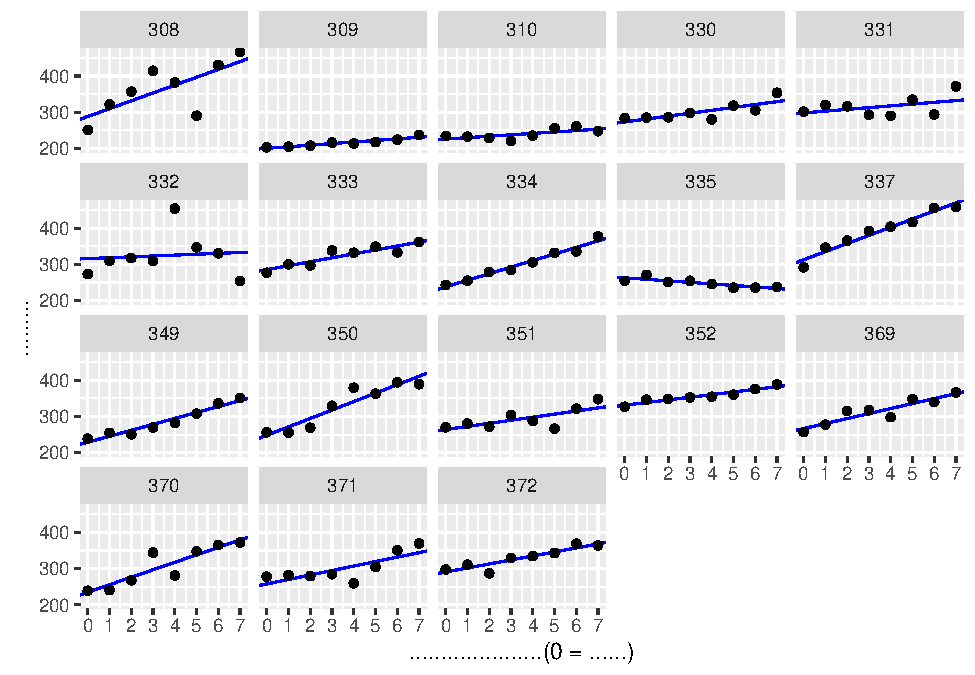
\includegraphics{05-介绍线性混合效应模型_files/figure-latex/np-model-fits-1.pdf}
\caption{\label{fig:np-model-fits}原始数据和不混合方法的拟合结果对比图}
\end{figure}

这比完全混合模型要好得多。如果要检验固定斜率为0的原假设,可以用单样本检验。

\begin{Shaded}
\begin{Highlighting}[]
\NormalTok{np\_coef }\SpecialCharTok{\%\textgreater{}\%} \FunctionTok{pull}\NormalTok{(slope) }\SpecialCharTok{\%\textgreater{}\%} \FunctionTok{t.test}\NormalTok{()}
\end{Highlighting}
\end{Shaded}

\begin{verbatim}
## 
##  One Sample t-test
## 
## data:  .
## t = 6.1971, df = 17, p-value = 9.749e-06
## alternative hypothesis: true mean is not equal to 0
## 95 percent confidence interval:
##   7.542244 15.328613
## sample estimates:
## mean of x 
##  11.43543
\end{verbatim}

这告诉我们平均斜率
11.435
显著不等于0,
t(17) = 6.197, \(p < .001\).

\hypertarget{ux4f7fux7528ux6df7ux5408ux6548ux679cux6a21ux578bux7684ux90e8ux5206ux6df7ux5408}{%
\section{使用混合效果模型的部分混合}\label{ux4f7fux7528ux6df7ux5408ux6548ux679cux6a21ux578bux7684ux90e8ux5206ux6df7ux5408}}

完全混合或不混合方法都不是令人满意的。如果我们能够利用对其他被试的了解来改进对单个被试的估计,那将是可取的。这将有助于更好地区分每个被试的信号(signal)和误差(error),并提高对总体的可推广性。正如最下面的网页APP所示,当我们有不平衡或缺失的数据时,这变得尤为重要。

在不混合模型中,我们将\texttt{Subject}视为一个\textbf{固定因子(fixed factor)}。每对截距和斜率的估计仅由该被试的数据决定。然而,我们对这18个被试本身并不感兴趣;我们更感兴趣的是他们作为具有潜在被试的更大群体的代表。如果你的目标是推广到你感兴趣的群体中的新被试,那么这种被试作为固定效应因子的方法是不够优化的。

部分混合发生在你将一个因子视为随机因子而不是固定因子进行分析时。\textbf{随机因子(random factor)}是指其水平被认为代表所有潜在水平的一个真子集(proper subset)。通常情况下,当你数据中的水平是抽样结果,并且你希望推广到超出这些水平的范围时,你会将一个因子视为随机。在这种情况下,我们有18个独特被试(因此有18个\texttt{Subject}因子的水平),希望能够对潜在被试群体的睡眠剥夺效应做出一些一般性的陈述。

一种在分析中包含随机因子的方法是使用线性混合效应模型(linear mixed-effects model)。当你这样做时,每个因子水平(即每个被试)的估计值将受其他水平(即其他被试)信息的影响。与不考虑其他被试估计的情况下为每个被试估计截距和斜率相比,该模型会估计总体的值,并将各个被试的估计值向这些值拉近,这种统计现象称为\texttt{shrinkage}。

下面是多层模型。理解其中的数学原理及其意义非常重要。乍一看似乎很复杂,但实际上这里没有什么是你以前没有见过的。我们将逐步解释一切。

\emph{第1层:}

\begin{equation}
Y_{sd} = \beta_{0s} + \beta_{1s} X_{sd} + e_{sd}
\end{equation}

\emph{第2层:}

\begin{equation}
\beta_{0s} = \gamma_{0} + S_{0s}
\end{equation}

\begin{equation}
\beta_{1s} = \gamma_{1} + S_{1s}
\end{equation}

\emph{方差成分(variance components):}

\begin{equation}
 \langle S_{0s}, S_{1s} \rangle \sim N\left(\langle 0, 0 \rangle, \mathbf{\Sigma}\right) 
\end{equation}

\begin{equation}
\mathbf{\Sigma} = \left(\begin{array}{cc}{\tau_{00}}^2 & \rho\tau_{00}\tau_{11} \\
         \rho\tau_{00}\tau_{11} & {\tau_{11}}^2 \\
         \end{array}\right) 
\end{equation}

\begin{equation}
e_{sd} \sim N\left(0, \sigma^2\right)
\end{equation}

如果你感到迷惑,这里有一个表格,解释了上述方程组中的所有变量。

\begin{longtable}[]{@{}
  >{\raggedright\arraybackslash}p{(\columnwidth - 4\tabcolsep) * \real{0.2255}}
  >{\raggedright\arraybackslash}p{(\columnwidth - 4\tabcolsep) * \real{0.1176}}
  >{\raggedright\arraybackslash}p{(\columnwidth - 4\tabcolsep) * \real{0.6569}}@{}}
\toprule\noalign{}
\begin{minipage}[b]{\linewidth}\raggedright
变量
\end{minipage} & \begin{minipage}[b]{\linewidth}\raggedright
类型
\end{minipage} & \begin{minipage}[b]{\linewidth}\raggedright
描述
\end{minipage} \\
\midrule\noalign{}
\endhead
\bottomrule\noalign{}
\endlastfoot
\(Y_{sd}\) & 观测值 & 被试\(s\)在第\(d\)天的\texttt{Reaction}值 \\
\(X_{sd}\) & 观测值 & 被试\(s\)在第\(d\)天的\texttt{days\_deprived}值(0-7) \\
\(\beta_{0s}\) & 派生值 & 第1层截距参数 \\
\(\beta_{1s}\) & 派生值 & 第1层斜率参数 \\
\(e_{sd}\) & 派生值 & 被试\(s\)在第\(d\)天的误差 \\
\(\gamma_0\) & 固定 & 总体截距(``gamma'') \\
\(\gamma_1\) & 固定 & 总体斜率(``gamma'') \\
\(S_{0s}\) & 派生值 & 被试\(s\)的随机截距(偏移量) \\
\(S_{1s}\) & 派生值 & 被试\(s\)的随机斜率(偏移量) \\
\(\mathbf{\Sigma}\) & 随机 & 方差协方差矩阵 \\
\({\tau_{00}}^2\) & 随机 & 随机截距的方差 \\
\(\rho\) & 随机 & 截距和斜率之间的随机相关性 \\
\({\tau_{11}}^2\) & 随机 & 随机斜率的方差 \\
\(\sigma^2\) & 随机 & 误差方差 \\
\end{longtable}

注意,表格的``类型''列包含的内容有\emph{固定}、\emph{随机}和\emph{派生值}。尽管\emph{固定}和\emph{随机}是标准术语,但\emph{派生值}不是;我引入这个术语是为了帮助你理解这些不同变量在模型中的意义,并帮助你区分直接估计的变量和非直接估计的变量。

让我们从模型的第1层方程开始,它表示预测变量和响应变量之间的总体关系。它捕捉了反应时\(Y_{sd}\)和睡眠剥夺\(X_{sd}\)之间主要关系的函数形式:一条截距为\(\beta_{0s}\)和斜率为\(\beta_{1s}\)的直线。现在\(\beta_{0s}\)和\(\beta_{1s}\)使它看起来像完全混合模型,在这种模型中,我们为整个数据集估计一个截距和一个斜率;然而,我们实际上并没有直接估计这些值。相反,我们将\(\beta_{0s}\)和\(\beta_{1s}\)视为派生值:它们完全由模型第2层的变量定义。

模型的第2层由两个方程定义,表示被试层次的关系。在这里,我们通过固定效应\(\gamma_0\)和\emph{随机截距}\(S_{0s}\)来定义截距\(\beta_{0s}\);同样地,我们通过固定斜率\(\gamma_1\)和\emph{随机斜率}\(S_{1s}\)来定义斜率\(\beta_{1s}\)。

最后的方程代表模型的\emph{方差成分}。我们将在下面更详细地讨论这一点。

让我们将第2层方程代入第1层方程,看看以多层的方式表示的优势。

\begin{equation}
Y_{sd} = \gamma_{0} + S_{0s} + \left(\gamma_{1} + S_{1s}\right) X_{sd} + e_{sd}
\end{equation}

虽然``组合''公式语法在这种特定情况下足够容易理解,但多层的形式更清楚地向我们展示了模型的功能形式:一条直线。我们可以轻松地改变功能形式,例如捕捉非线性趋势:

\[Y_{sd} = \beta_{0s} + \beta_{1s} X_{sd} + \beta_{2s} X_{sd}^2 + e_{sd}\]

这种功能形式在组合语法中变得模糊不清。多层语法还使得容易看清哪些项与截距相关,哪些项与斜率相关。而且,随着设计变得更加复杂------例如,如果我们将被试分配到不同的实验条件中,在第2层就要引入更多的预测变量------组合方程将变得越来越难以解析和理解。

固定效应参数如\(\gamma_0\)和\(\gamma_1\)是从数据中估计得到的,反映了总体的稳定特性。在这个例子中,\(\gamma_0\)是总体截距,\(\gamma_1\)是总体斜率。你可以将这些\textbf{固定效应参数}视为代表总体中的\textbf{平均截距和斜率}。这些是``固定''的,因为我们假设它们反映了总体中的真实潜在值(underlying value);我们假设它们不会随着样本的变化而变。这些固定效应参数通常是主要的理论关注点;我们希望在数据允许的情况下,以一种尽可能公正和精确的方式来衡量它们和它们的标准差。在实验设置中,它们通常是假设检验的目标。

随机效应如\(S_{0i}\)和\(S_{1i}\)分别允许截距和斜率在不同被试之间变化。这些随机效应是\emph{偏移量}:相对于总体``总体均值''的偏差。有些被试的反应就是比别人慢,因此他们在第0天的截距(mean RT)高于总计估计值\(\hat{\gamma_0}\)。这些比平均速度更慢的被试会有正的\(S_{0i}\)值;比平均速度更快的被试会有负的\(S_{0i}\)值。同样,一些被试的睡眠剥夺效应比估计的总体效应\(\hat{\gamma_1}\)更强(更陡的斜率),这意味着正的偏移量\(S_{1s}\),而另一些可能显示出较弱的效应或几乎没有效应(负的偏移量)。

每个被试都可以表示为一个向量对\(\langle S_{0i}, S_{1i} \rangle\)。如果我们的样本中的被试包含了整个总体,我们将有理由将其视为固定效应并估计它们的值,像上文的``无混合''方法那样。然而情况并非如此。鉴于它们是抽样而来的,我们把被试视为随机因子而不是固定因子。我们不会估计我们恰好选中的被试的值,而是估计\textbf{代表这些值的二元分布的协方差矩阵}。通过这样做,我们允许样本中的被试向我们提供有关总体特征的信息。

\hypertarget{ux65b9ux5dee-ux534fux65b9ux5deeux77e9ux9635}{%
\subsection{方差-协方差矩阵}\label{ux65b9ux5dee-ux534fux65b9ux5deeux77e9ux9635}}

\begin{equation}
 \langle S_{0s}, S_{1s} \rangle \sim N\left(\langle 0, 0 \rangle, \mathbf{\Sigma}\right) 
\end{equation}

\begin{equation}
\mathbf{\Sigma} = \left(\begin{array}{cc}{\tau_{00}}^2 & \rho\tau_{00}\tau_{11} \\
         \rho\tau_{00}\tau_{11} & {\tau_{11}}^2 \\
         \end{array}\right) 
\end{equation}

\emph{方差分量}中的方程描述了我们对变异性(variability)的估计。第一个方程说明了我们的假设,即随机截距/随机斜率对\(\langle S_{0s}, S_{1s} \rangle\)是从一个二元正态分布中抽取的,该分布根据\(\mathbf{\Sigma}\)以原点\(\langle 0, 0 \rangle\)为中心。

协方差矩阵是关键:它决定了从总体中抽取随机效应对\(\langle S_{0s}, S_{1s} \rangle\)的概率。你在\protect\hyperlink{ux76f8ux5173ux548cux56deux5f52}{相关和回归}一章中已经见过这些。协方差矩阵总是一个方阵(列数和行数相等)。主对角线(左上角和右下角的单元格)表示随机效应方差\({\tau_{00}}^2\)和\({\tau_{11}}^2\)。\({\tau_{00}}^2\)是随机截距方差,它捕捉了被试在第0天(没有任何睡眠剥夺前)的平均反应时的变化程度。\({\tau_{11}}^2\)是随机斜率方差,它捕捉了被试对睡眠剥夺效应敏感性的变化程度。

非对角线的单元格包含协方差,但这些信息在矩阵中是冗余表示;左下角元素与右上角元素相同,两者都捕捉了随机截距和斜率之间的协方差,如\(\rho\tau_{00}\tau_{11}\)所示。在这个方程中,\(\rho\)是截距和斜率之间的相关性。因此,矩阵中的所有信息都可以通过三个参数来捕捉:\(\tau_{00}\)、\(\tau_{11}\)和\(\rho\)。

\hypertarget{ux4f30ux8ba1ux6a21ux578bux53c2ux6570}{%
\section{估计模型参数}\label{ux4f30ux8ba1ux6a21ux578bux53c2ux6570}}

为了估计参数,我们将使用lme4包的\texttt{lmer()}函数\citep{Bates_et_al_2015}。\texttt{lmer()}的基本公式如下:

\begin{verbatim}
lmer(formula, data, ...)
\end{verbatim}

其中\texttt{formula}以精简的形式表示底层模型的结构,\texttt{data}是\texttt{formula}中提到的变量所在的数据框。

N个固定效应(\texttt{fix})和K个随机效应(\texttt{ran})的模型公式一般格式为:

\texttt{DV\ \textasciitilde{}\ fix1\ +\ fix2\ +\ ...\ +\ fixN\ +\ (ran1\ +\ ran2\ +\ ...\ +\ ranK\ \textbar{}\ random\_factor1)}

因子A和因子B之间的交互效应可以用\texttt{A\ *\ B}(交互效应和主效应)或\texttt{A:B}(仅仅是交互效应)来指定。

与标准的R模型语法的一个关键区别是存在一个随机效应项,该项在括号内,即\texttt{(ran1\ +\ ran2\ +\ ...\ +\ ranK\ \textbar{}\ random\_factor)}。每个括号中的表达式表示与单个随机因子相关的随机效应。当我们讨论交叉随机因子时,你会看到在一个公式中可以有多个随机效应项。你应该将随机效应项看作为\texttt{lmer()}提供\textbf{构造方差-协方差矩阵的指示}。

在竖线\texttt{\textbar{}}的左侧(注:建议大家了解一下英文中符号的表达,如\texttt{\textbar{}}是竖线,bar;\texttt{/}是正斜杠或除号,forward slash或division sign;\texttt{\textbackslash{}}是反斜杠,backward slash,有时也用backslash等,这样便于阅读技术手册和工作交流),放置你希望允许随右侧随机因子的不同水平变化的效应。通常右边的变量是可以唯一地标识单个被试的变量(如\texttt{subject\_id})。

考虑下方\texttt{sleep2}数据的可能模型公式及其构造的方差-协方差矩阵。

\begin{longtable}[]{@{}
  >{\raggedright\arraybackslash}p{(\columnwidth - 4\tabcolsep) * \real{0.0286}}
  >{\raggedright\arraybackslash}p{(\columnwidth - 4\tabcolsep) * \real{0.3524}}
  >{\raggedright\arraybackslash}p{(\columnwidth - 4\tabcolsep) * \real{0.6190}}@{}}
\toprule\noalign{}
\begin{minipage}[b]{\linewidth}\raggedright
\end{minipage} & \begin{minipage}[b]{\linewidth}\raggedright
模型
\end{minipage} & \begin{minipage}[b]{\linewidth}\raggedright
语法
\end{minipage} \\
\midrule\noalign{}
\endhead
\bottomrule\noalign{}
\endlastfoot
1 & 仅随机截距 & \texttt{Reaction\ \textasciitilde{}\ days\_deprived\ +\ (1\ \textbar{}\ Subject)} \\
2 & 随机截距和斜率 & \texttt{Reaction\ \textasciitilde{}\ days\_deprived\ +\ (1\ +\ days\_deprived\ \textbar{}\ Subject)} \\
3 & 模型2的备选语法 & \texttt{Reaction\ \textasciitilde{}\ days\_deprived\ +\ (days\_deprived\ \textbar{}\ Subject)} \\
4 & 仅随机斜率 & \texttt{Reaction\ \textasciitilde{}\ days\_deprived\ +\ (0\ +\ days\_deprived\ \textbar{}\ Subject)} \\
5 & 模型2 + 0协方差(zero-covariances) & \texttt{Reaction\ \textasciitilde{}\ days\_deprived\ +\ (days\_deprived\ \textbar{}\textbar{}\ Subject)} \\
\end{longtable}

\emph{模型1:}

\begin{equation*}
  \mathbf{\Sigma} = \left(
  \begin{array}{cc}
    {\tau_{00}}^2 & 0 \\
                0 & 0 \\
  \end{array}\right) 
\end{equation*}

\emph{模型2和3:}

\begin{equation*}
  \mathbf{\Sigma} = \left(
  \begin{array}{cc}
             {\tau_{00}}^2 & \rho\tau_{00}\tau_{11} \\
    \rho\tau_{00}\tau_{11} &          {\tau_{11}}^2 \\
  \end{array}\right) 
\end{equation*}

\emph{模型4:}

\begin{equation*}
  \mathbf{\Sigma} = \left(
  \begin{array}{cc}
    0 &             0 \\
    0 & {\tau_{11}}^2 \\
  \end{array}\right) 
\end{equation*}

\emph{模型5:}

\begin{equation*}
  \mathbf{\Sigma} = \left(
  \begin{array}{cc}
    {\tau_{00}}^2 &             0 \\
                0 & {\tau_{11}}^2 \\
  \end{array}\right) 
\end{equation*}

对于这些数据来说,最合理的模型是模型2,所以我们继续使用它。

让我们拟合模型,将结果存储在\texttt{pp\_mod}中。

\begin{Shaded}
\begin{Highlighting}[]
\NormalTok{pp\_mod }\OtherTok{\textless{}{-}} \FunctionTok{lmer}\NormalTok{(Reaction }\SpecialCharTok{\textasciitilde{}}\NormalTok{ days\_deprived }\SpecialCharTok{+}\NormalTok{ (days\_deprived }\SpecialCharTok{|}\NormalTok{ Subject), sleep2)}

\FunctionTok{summary}\NormalTok{(pp\_mod)}
\end{Highlighting}
\end{Shaded}

\begin{verbatim}
## Linear mixed model fit by REML ['lmerMod']
## Formula: Reaction ~ days_deprived + (days_deprived | Subject)
##    Data: sleep2
## 
## REML criterion at convergence: 1404.1
## 
## Scaled residuals: 
##     Min      1Q  Median      3Q     Max 
## -4.0157 -0.3541  0.0069  0.4681  5.0732 
## 
## Random effects:
##  Groups   Name          Variance Std.Dev. Corr
##  Subject  (Intercept)   958.35   30.957       
##           days_deprived  45.78    6.766   0.18
##  Residual               651.60   25.526       
## Number of obs: 144, groups:  Subject, 18
## 
## Fixed effects:
##               Estimate Std. Error t value
## (Intercept)    267.967      8.266  32.418
## days_deprived   11.435      1.845   6.197
## 
## Correlation of Fixed Effects:
##             (Intr)
## days_deprvd -0.062
\end{verbatim}

在讨论如何解释输出结果之前,我们先绘制原始数据与模型预测值的对比图。我们可以使用\texttt{predict()}函数获取模型预测值(有关与混合效应模型一起使用的更多信息,参见\texttt{?predict.merMod})。

首先为\texttt{Subject}和\texttt{days\_deprivation}的预测值创建一个新的数据集。

\begin{Shaded}
\begin{Highlighting}[]
\NormalTok{newdata }\OtherTok{\textless{}{-}} \FunctionTok{crossing}\NormalTok{(}
  \AttributeTok{Subject =}\NormalTok{ sleep2 }\SpecialCharTok{\%\textgreater{}\%} \FunctionTok{pull}\NormalTok{(Subject) }\SpecialCharTok{\%\textgreater{}\%} \FunctionTok{levels}\NormalTok{() }\SpecialCharTok{\%\textgreater{}\%} \FunctionTok{factor}\NormalTok{(),}
  \AttributeTok{days\_deprived =} \DecValTok{0}\SpecialCharTok{:}\DecValTok{7}\NormalTok{)}

\FunctionTok{head}\NormalTok{(newdata, }\DecValTok{17}\NormalTok{)}
\end{Highlighting}
\end{Shaded}

\begin{verbatim}
## # A tibble: 17 x 2
##    Subject days_deprived
##    <fct>           <int>
##  1 308                 0
##  2 308                 1
##  3 308                 2
##  4 308                 3
##  5 308                 4
##  6 308                 5
##  7 308                 6
##  8 308                 7
##  9 309                 0
## 10 309                 1
## 11 309                 2
## 12 309                 3
## 13 309                 4
## 14 309                 5
## 15 309                 6
## 16 309                 7
## 17 310                 0
\end{verbatim}

然后,通过\texttt{predict()}运行这个数据框。通常我们会将预测值作为新变量添加到新的数据框中,并将其命名为与我们的因变量(\texttt{Reaction})相同的名称。

\begin{Shaded}
\begin{Highlighting}[]
\NormalTok{newdata2 }\OtherTok{\textless{}{-}}\NormalTok{ newdata }\SpecialCharTok{\%\textgreater{}\%}
  \FunctionTok{mutate}\NormalTok{(}\AttributeTok{Reaction =} \FunctionTok{predict}\NormalTok{(pp\_mod, newdata))}
\end{Highlighting}
\end{Shaded}

现在我们准备好绘图了。

\begin{Shaded}
\begin{Highlighting}[]
\FunctionTok{ggplot}\NormalTok{(sleep2, }\FunctionTok{aes}\NormalTok{(}\AttributeTok{x =}\NormalTok{ days\_deprived, }\AttributeTok{y =}\NormalTok{ Reaction)) }\SpecialCharTok{+}
  \FunctionTok{geom\_line}\NormalTok{(}\AttributeTok{data =}\NormalTok{ newdata2,}
            \AttributeTok{color =} \StringTok{\textquotesingle{}blue\textquotesingle{}}\NormalTok{) }\SpecialCharTok{+}
  \FunctionTok{geom\_point}\NormalTok{() }\SpecialCharTok{+}
  \FunctionTok{scale\_x\_continuous}\NormalTok{(}\AttributeTok{breaks =} \DecValTok{0}\SpecialCharTok{:}\DecValTok{7}\NormalTok{) }\SpecialCharTok{+}
  \FunctionTok{facet\_wrap}\NormalTok{(}\SpecialCharTok{\textasciitilde{}}\NormalTok{Subject) }\SpecialCharTok{+}
  \FunctionTok{labs}\NormalTok{(}\AttributeTok{y =} \StringTok{"反应时"}\NormalTok{, }\AttributeTok{x =} \StringTok{"睡眠剥夺的天数(0 = 基线)"}\NormalTok{)}
\end{Highlighting}
\end{Shaded}

\begin{verbatim}
## Warning in grid.Call(C_textBounds, as.graphicsAnnot(x$label), x$x, x$y, :
## conversion failure on '反应时' in 'mbcsToSbcs': dot substituted for <e5>
\end{verbatim}

\begin{verbatim}
## Warning in grid.Call(C_textBounds, as.graphicsAnnot(x$label), x$x, x$y, :
## conversion failure on '反应时' in 'mbcsToSbcs': dot substituted for <8f>
\end{verbatim}

\begin{verbatim}
## Warning in grid.Call(C_textBounds, as.graphicsAnnot(x$label), x$x, x$y, :
## conversion failure on '反应时' in 'mbcsToSbcs': dot substituted for <8d>
\end{verbatim}

\begin{verbatim}
## Warning in grid.Call(C_textBounds, as.graphicsAnnot(x$label), x$x, x$y, :
## conversion failure on '反应时' in 'mbcsToSbcs': dot substituted for <e5>
\end{verbatim}

\begin{verbatim}
## Warning in grid.Call(C_textBounds, as.graphicsAnnot(x$label), x$x, x$y, :
## conversion failure on '反应时' in 'mbcsToSbcs': dot substituted for <ba>
\end{verbatim}

\begin{verbatim}
## Warning in grid.Call(C_textBounds, as.graphicsAnnot(x$label), x$x, x$y, :
## conversion failure on '反应时' in 'mbcsToSbcs': dot substituted for <94>
\end{verbatim}

\begin{verbatim}
## Warning in grid.Call(C_textBounds, as.graphicsAnnot(x$label), x$x, x$y, :
## conversion failure on '反应时' in 'mbcsToSbcs': dot substituted for <e6>
\end{verbatim}

\begin{verbatim}
## Warning in grid.Call(C_textBounds, as.graphicsAnnot(x$label), x$x, x$y, :
## conversion failure on '反应时' in 'mbcsToSbcs': dot substituted for <97>
\end{verbatim}

\begin{verbatim}
## Warning in grid.Call(C_textBounds, as.graphicsAnnot(x$label), x$x, x$y, :
## conversion failure on '反应时' in 'mbcsToSbcs': dot substituted for <b6>
\end{verbatim}

\begin{verbatim}
## Warning in grid.Call(C_textBounds, as.graphicsAnnot(x$label), x$x, x$y, :
## conversion failure on '睡眠剥夺的天数(0 = 基线)' in 'mbcsToSbcs': dot
## substituted for <e7>
\end{verbatim}

\begin{verbatim}
## Warning in grid.Call(C_textBounds, as.graphicsAnnot(x$label), x$x, x$y, :
## conversion failure on '睡眠剥夺的天数(0 = 基线)' in 'mbcsToSbcs': dot
## substituted for <9d>
\end{verbatim}

\begin{verbatim}
## Warning in grid.Call(C_textBounds, as.graphicsAnnot(x$label), x$x, x$y, :
## conversion failure on '睡眠剥夺的天数(0 = 基线)' in 'mbcsToSbcs': dot
## substituted for <a1>
\end{verbatim}

\begin{verbatim}
## Warning in grid.Call(C_textBounds, as.graphicsAnnot(x$label), x$x, x$y, :
## conversion failure on '睡眠剥夺的天数(0 = 基线)' in 'mbcsToSbcs': dot
## substituted for <e7>
\end{verbatim}

\begin{verbatim}
## Warning in grid.Call(C_textBounds, as.graphicsAnnot(x$label), x$x, x$y, :
## conversion failure on '睡眠剥夺的天数(0 = 基线)' in 'mbcsToSbcs': dot
## substituted for <9c>
\end{verbatim}

\begin{verbatim}
## Warning in grid.Call(C_textBounds, as.graphicsAnnot(x$label), x$x, x$y, :
## conversion failure on '睡眠剥夺的天数(0 = 基线)' in 'mbcsToSbcs': dot
## substituted for <a0>
\end{verbatim}

\begin{verbatim}
## Warning in grid.Call(C_textBounds, as.graphicsAnnot(x$label), x$x, x$y, :
## conversion failure on '睡眠剥夺的天数(0 = 基线)' in 'mbcsToSbcs': dot
## substituted for <e5>
\end{verbatim}

\begin{verbatim}
## Warning in grid.Call(C_textBounds, as.graphicsAnnot(x$label), x$x, x$y, :
## conversion failure on '睡眠剥夺的天数(0 = 基线)' in 'mbcsToSbcs': dot
## substituted for <89>
\end{verbatim}

\begin{verbatim}
## Warning in grid.Call(C_textBounds, as.graphicsAnnot(x$label), x$x, x$y, :
## conversion failure on '睡眠剥夺的天数(0 = 基线)' in 'mbcsToSbcs': dot
## substituted for <a5>
\end{verbatim}

\begin{verbatim}
## Warning in grid.Call(C_textBounds, as.graphicsAnnot(x$label), x$x, x$y, :
## conversion failure on '睡眠剥夺的天数(0 = 基线)' in 'mbcsToSbcs': dot
## substituted for <e5>
\end{verbatim}

\begin{verbatim}
## Warning in grid.Call(C_textBounds, as.graphicsAnnot(x$label), x$x, x$y, :
## conversion failure on '睡眠剥夺的天数(0 = 基线)' in 'mbcsToSbcs': dot
## substituted for <a4>
\end{verbatim}

\begin{verbatim}
## Warning in grid.Call(C_textBounds, as.graphicsAnnot(x$label), x$x, x$y, :
## conversion failure on '睡眠剥夺的天数(0 = 基线)' in 'mbcsToSbcs': dot
## substituted for <ba>
\end{verbatim}

\begin{verbatim}
## Warning in grid.Call(C_textBounds, as.graphicsAnnot(x$label), x$x, x$y, :
## conversion failure on '睡眠剥夺的天数(0 = 基线)' in 'mbcsToSbcs': dot
## substituted for <e7>
\end{verbatim}

\begin{verbatim}
## Warning in grid.Call(C_textBounds, as.graphicsAnnot(x$label), x$x, x$y, :
## conversion failure on '睡眠剥夺的天数(0 = 基线)' in 'mbcsToSbcs': dot
## substituted for <9a>
\end{verbatim}

\begin{verbatim}
## Warning in grid.Call(C_textBounds, as.graphicsAnnot(x$label), x$x, x$y, :
## conversion failure on '睡眠剥夺的天数(0 = 基线)' in 'mbcsToSbcs': dot
## substituted for <84>
\end{verbatim}

\begin{verbatim}
## Warning in grid.Call(C_textBounds, as.graphicsAnnot(x$label), x$x, x$y, :
## conversion failure on '睡眠剥夺的天数(0 = 基线)' in 'mbcsToSbcs': dot
## substituted for <e5>
\end{verbatim}

\begin{verbatim}
## Warning in grid.Call(C_textBounds, as.graphicsAnnot(x$label), x$x, x$y, :
## conversion failure on '睡眠剥夺的天数(0 = 基线)' in 'mbcsToSbcs': dot
## substituted for <a4>
\end{verbatim}

\begin{verbatim}
## Warning in grid.Call(C_textBounds, as.graphicsAnnot(x$label), x$x, x$y, :
## conversion failure on '睡眠剥夺的天数(0 = 基线)' in 'mbcsToSbcs': dot
## substituted for <a9>
\end{verbatim}

\begin{verbatim}
## Warning in grid.Call(C_textBounds, as.graphicsAnnot(x$label), x$x, x$y, :
## conversion failure on '睡眠剥夺的天数(0 = 基线)' in 'mbcsToSbcs': dot
## substituted for <e6>
\end{verbatim}

\begin{verbatim}
## Warning in grid.Call(C_textBounds, as.graphicsAnnot(x$label), x$x, x$y, :
## conversion failure on '睡眠剥夺的天数(0 = 基线)' in 'mbcsToSbcs': dot
## substituted for <95>
\end{verbatim}

\begin{verbatim}
## Warning in grid.Call(C_textBounds, as.graphicsAnnot(x$label), x$x, x$y, :
## conversion failure on '睡眠剥夺的天数(0 = 基线)' in 'mbcsToSbcs': dot
## substituted for <b0>
\end{verbatim}

\begin{verbatim}
## Warning in grid.Call(C_textBounds, as.graphicsAnnot(x$label), x$x, x$y, :
## conversion failure on '睡眠剥夺的天数(0 = 基线)' in 'mbcsToSbcs': dot
## substituted for <e5>
\end{verbatim}

\begin{verbatim}
## Warning in grid.Call(C_textBounds, as.graphicsAnnot(x$label), x$x, x$y, :
## conversion failure on '睡眠剥夺的天数(0 = 基线)' in 'mbcsToSbcs': dot
## substituted for <9f>
\end{verbatim}

\begin{verbatim}
## Warning in grid.Call(C_textBounds, as.graphicsAnnot(x$label), x$x, x$y, :
## conversion failure on '睡眠剥夺的天数(0 = 基线)' in 'mbcsToSbcs': dot
## substituted for <ba>
\end{verbatim}

\begin{verbatim}
## Warning in grid.Call(C_textBounds, as.graphicsAnnot(x$label), x$x, x$y, :
## conversion failure on '睡眠剥夺的天数(0 = 基线)' in 'mbcsToSbcs': dot
## substituted for <e7>
\end{verbatim}

\begin{verbatim}
## Warning in grid.Call(C_textBounds, as.graphicsAnnot(x$label), x$x, x$y, :
## conversion failure on '睡眠剥夺的天数(0 = 基线)' in 'mbcsToSbcs': dot
## substituted for <ba>
\end{verbatim}

\begin{verbatim}
## Warning in grid.Call(C_textBounds, as.graphicsAnnot(x$label), x$x, x$y, :
## conversion failure on '睡眠剥夺的天数(0 = 基线)' in 'mbcsToSbcs': dot
## substituted for <bf>
\end{verbatim}

\begin{verbatim}
## Warning in grid.Call.graphics(C_text, as.graphicsAnnot(x$label), x$x, x$y, :
## conversion failure on '睡眠剥夺的天数(0 = 基线)' in 'mbcsToSbcs': dot
## substituted for <e7>
\end{verbatim}

\begin{verbatim}
## Warning in grid.Call.graphics(C_text, as.graphicsAnnot(x$label), x$x, x$y, :
## conversion failure on '睡眠剥夺的天数(0 = 基线)' in 'mbcsToSbcs': dot
## substituted for <9d>
\end{verbatim}

\begin{verbatim}
## Warning in grid.Call.graphics(C_text, as.graphicsAnnot(x$label), x$x, x$y, :
## conversion failure on '睡眠剥夺的天数(0 = 基线)' in 'mbcsToSbcs': dot
## substituted for <a1>
\end{verbatim}

\begin{verbatim}
## Warning in grid.Call.graphics(C_text, as.graphicsAnnot(x$label), x$x, x$y, :
## conversion failure on '睡眠剥夺的天数(0 = 基线)' in 'mbcsToSbcs': dot
## substituted for <e7>
\end{verbatim}

\begin{verbatim}
## Warning in grid.Call.graphics(C_text, as.graphicsAnnot(x$label), x$x, x$y, :
## conversion failure on '睡眠剥夺的天数(0 = 基线)' in 'mbcsToSbcs': dot
## substituted for <9c>
\end{verbatim}

\begin{verbatim}
## Warning in grid.Call.graphics(C_text, as.graphicsAnnot(x$label), x$x, x$y, :
## conversion failure on '睡眠剥夺的天数(0 = 基线)' in 'mbcsToSbcs': dot
## substituted for <a0>
\end{verbatim}

\begin{verbatim}
## Warning in grid.Call.graphics(C_text, as.graphicsAnnot(x$label), x$x, x$y, :
## conversion failure on '睡眠剥夺的天数(0 = 基线)' in 'mbcsToSbcs': dot
## substituted for <e5>
\end{verbatim}

\begin{verbatim}
## Warning in grid.Call.graphics(C_text, as.graphicsAnnot(x$label), x$x, x$y, :
## conversion failure on '睡眠剥夺的天数(0 = 基线)' in 'mbcsToSbcs': dot
## substituted for <89>
\end{verbatim}

\begin{verbatim}
## Warning in grid.Call.graphics(C_text, as.graphicsAnnot(x$label), x$x, x$y, :
## conversion failure on '睡眠剥夺的天数(0 = 基线)' in 'mbcsToSbcs': dot
## substituted for <a5>
\end{verbatim}

\begin{verbatim}
## Warning in grid.Call.graphics(C_text, as.graphicsAnnot(x$label), x$x, x$y, :
## conversion failure on '睡眠剥夺的天数(0 = 基线)' in 'mbcsToSbcs': dot
## substituted for <e5>
\end{verbatim}

\begin{verbatim}
## Warning in grid.Call.graphics(C_text, as.graphicsAnnot(x$label), x$x, x$y, :
## conversion failure on '睡眠剥夺的天数(0 = 基线)' in 'mbcsToSbcs': dot
## substituted for <a4>
\end{verbatim}

\begin{verbatim}
## Warning in grid.Call.graphics(C_text, as.graphicsAnnot(x$label), x$x, x$y, :
## conversion failure on '睡眠剥夺的天数(0 = 基线)' in 'mbcsToSbcs': dot
## substituted for <ba>
\end{verbatim}

\begin{verbatim}
## Warning in grid.Call.graphics(C_text, as.graphicsAnnot(x$label), x$x, x$y, :
## conversion failure on '睡眠剥夺的天数(0 = 基线)' in 'mbcsToSbcs': dot
## substituted for <e7>
\end{verbatim}

\begin{verbatim}
## Warning in grid.Call.graphics(C_text, as.graphicsAnnot(x$label), x$x, x$y, :
## conversion failure on '睡眠剥夺的天数(0 = 基线)' in 'mbcsToSbcs': dot
## substituted for <9a>
\end{verbatim}

\begin{verbatim}
## Warning in grid.Call.graphics(C_text, as.graphicsAnnot(x$label), x$x, x$y, :
## conversion failure on '睡眠剥夺的天数(0 = 基线)' in 'mbcsToSbcs': dot
## substituted for <84>
\end{verbatim}

\begin{verbatim}
## Warning in grid.Call.graphics(C_text, as.graphicsAnnot(x$label), x$x, x$y, :
## conversion failure on '睡眠剥夺的天数(0 = 基线)' in 'mbcsToSbcs': dot
## substituted for <e5>
\end{verbatim}

\begin{verbatim}
## Warning in grid.Call.graphics(C_text, as.graphicsAnnot(x$label), x$x, x$y, :
## conversion failure on '睡眠剥夺的天数(0 = 基线)' in 'mbcsToSbcs': dot
## substituted for <a4>
\end{verbatim}

\begin{verbatim}
## Warning in grid.Call.graphics(C_text, as.graphicsAnnot(x$label), x$x, x$y, :
## conversion failure on '睡眠剥夺的天数(0 = 基线)' in 'mbcsToSbcs': dot
## substituted for <a9>
\end{verbatim}

\begin{verbatim}
## Warning in grid.Call.graphics(C_text, as.graphicsAnnot(x$label), x$x, x$y, :
## conversion failure on '睡眠剥夺的天数(0 = 基线)' in 'mbcsToSbcs': dot
## substituted for <e6>
\end{verbatim}

\begin{verbatim}
## Warning in grid.Call.graphics(C_text, as.graphicsAnnot(x$label), x$x, x$y, :
## conversion failure on '睡眠剥夺的天数(0 = 基线)' in 'mbcsToSbcs': dot
## substituted for <95>
\end{verbatim}

\begin{verbatim}
## Warning in grid.Call.graphics(C_text, as.graphicsAnnot(x$label), x$x, x$y, :
## conversion failure on '睡眠剥夺的天数(0 = 基线)' in 'mbcsToSbcs': dot
## substituted for <b0>
\end{verbatim}

\begin{verbatim}
## Warning in grid.Call.graphics(C_text, as.graphicsAnnot(x$label), x$x, x$y, :
## conversion failure on '睡眠剥夺的天数(0 = 基线)' in 'mbcsToSbcs': dot
## substituted for <e5>
\end{verbatim}

\begin{verbatim}
## Warning in grid.Call.graphics(C_text, as.graphicsAnnot(x$label), x$x, x$y, :
## conversion failure on '睡眠剥夺的天数(0 = 基线)' in 'mbcsToSbcs': dot
## substituted for <9f>
\end{verbatim}

\begin{verbatim}
## Warning in grid.Call.graphics(C_text, as.graphicsAnnot(x$label), x$x, x$y, :
## conversion failure on '睡眠剥夺的天数(0 = 基线)' in 'mbcsToSbcs': dot
## substituted for <ba>
\end{verbatim}

\begin{verbatim}
## Warning in grid.Call.graphics(C_text, as.graphicsAnnot(x$label), x$x, x$y, :
## conversion failure on '睡眠剥夺的天数(0 = 基线)' in 'mbcsToSbcs': dot
## substituted for <e7>
\end{verbatim}

\begin{verbatim}
## Warning in grid.Call.graphics(C_text, as.graphicsAnnot(x$label), x$x, x$y, :
## conversion failure on '睡眠剥夺的天数(0 = 基线)' in 'mbcsToSbcs': dot
## substituted for <ba>
\end{verbatim}

\begin{verbatim}
## Warning in grid.Call.graphics(C_text, as.graphicsAnnot(x$label), x$x, x$y, :
## conversion failure on '睡眠剥夺的天数(0 = 基线)' in 'mbcsToSbcs': dot
## substituted for <bf>
\end{verbatim}

\begin{verbatim}
## Warning in grid.Call.graphics(C_text, as.graphicsAnnot(x$label), x$x, x$y, :
## conversion failure on '反应时' in 'mbcsToSbcs': dot substituted for <e5>
\end{verbatim}

\begin{verbatim}
## Warning in grid.Call.graphics(C_text, as.graphicsAnnot(x$label), x$x, x$y, :
## conversion failure on '反应时' in 'mbcsToSbcs': dot substituted for <8f>
\end{verbatim}

\begin{verbatim}
## Warning in grid.Call.graphics(C_text, as.graphicsAnnot(x$label), x$x, x$y, :
## conversion failure on '反应时' in 'mbcsToSbcs': dot substituted for <8d>
\end{verbatim}

\begin{verbatim}
## Warning in grid.Call.graphics(C_text, as.graphicsAnnot(x$label), x$x, x$y, :
## conversion failure on '反应时' in 'mbcsToSbcs': dot substituted for <e5>
\end{verbatim}

\begin{verbatim}
## Warning in grid.Call.graphics(C_text, as.graphicsAnnot(x$label), x$x, x$y, :
## conversion failure on '反应时' in 'mbcsToSbcs': dot substituted for <ba>
\end{verbatim}

\begin{verbatim}
## Warning in grid.Call.graphics(C_text, as.graphicsAnnot(x$label), x$x, x$y, :
## conversion failure on '反应时' in 'mbcsToSbcs': dot substituted for <94>
\end{verbatim}

\begin{verbatim}
## Warning in grid.Call.graphics(C_text, as.graphicsAnnot(x$label), x$x, x$y, :
## conversion failure on '反应时' in 'mbcsToSbcs': dot substituted for <e6>
\end{verbatim}

\begin{verbatim}
## Warning in grid.Call.graphics(C_text, as.graphicsAnnot(x$label), x$x, x$y, :
## conversion failure on '反应时' in 'mbcsToSbcs': dot substituted for <97>
\end{verbatim}

\begin{verbatim}
## Warning in grid.Call.graphics(C_text, as.graphicsAnnot(x$label), x$x, x$y, :
## conversion failure on '反应时' in 'mbcsToSbcs': dot substituted for <b6>
\end{verbatim}

\begin{figure}
\centering
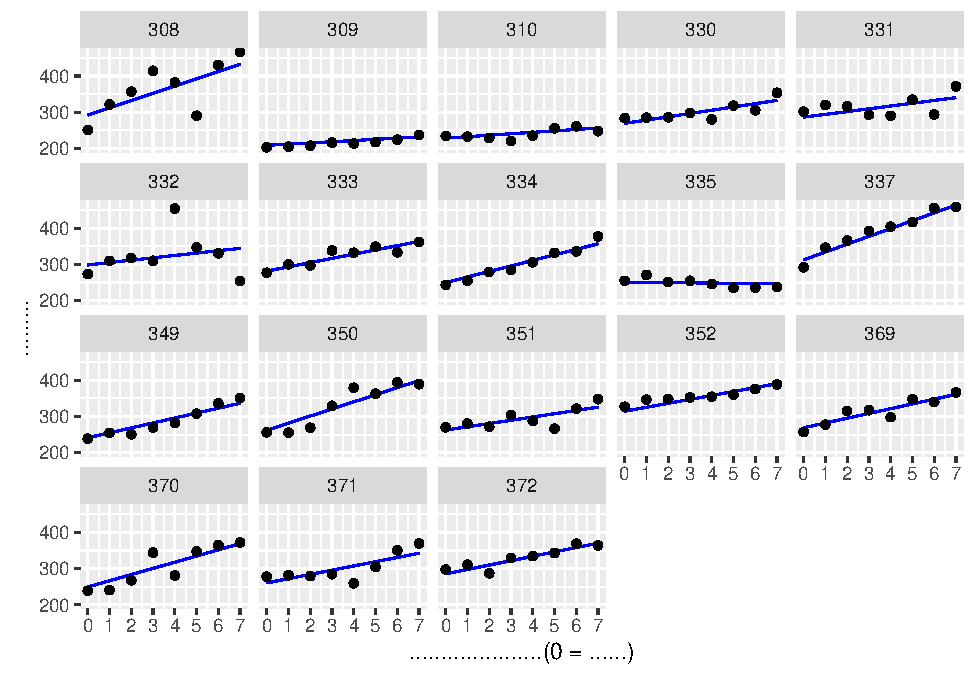
\includegraphics{05-介绍线性混合效应模型_files/figure-latex/pp-plot-1.pdf}
\caption{\label{fig:pp-plot}原始数据和部分混合方法的拟合结果对比图}
\end{figure}

\hypertarget{ux89e3ux91calmerux8f93ux51faux7ed3ux679cux5e76ux63d0ux53d6ux4f30ux8ba1ux503c}{%
\section{\texorpdfstring{解释\texttt{lmer()}输出结果并提取估计值}{解释lmer()输出结果并提取估计值}}\label{ux89e3ux91calmerux8f93ux51faux7ed3ux679cux5e76ux63d0ux53d6ux4f30ux8ba1ux503c}}

调用\texttt{lmer()}返回一个''lmerMod''类的拟合模型对象。要了解有关\texttt{lmerMod}类(\texttt{merMod}类的一个特化版本)的更多信息,参见\texttt{?lmerMod-class}。

\hypertarget{ux56faux5b9aux6548ux5e94}{%
\subsection{固定效应}\label{ux56faux5b9aux6548ux5e94}}

输出中\texttt{Fixed\ effects:}部分应该看起来很熟悉;它类似于通过\texttt{lm()}拟合的简单线性模型输出结果中的内容。

\begin{verbatim}
## Fixed effects:
##               Estimate Std. Error t value
## (Intercept)    267.967      8.266  32.418
## days_deprived   11.435      1.845   6.197
\end{verbatim}

这表明,在第0天被试的反应时估计平均约为268毫秒,每增加1天睡眠剥夺平均增加11毫秒反应时。

如果我们需要从模型中获取固定效应,我们可以使用\texttt{fixef()}提取它们。

\begin{Shaded}
\begin{Highlighting}[]
\FunctionTok{fixef}\NormalTok{(pp\_mod)}
\end{Highlighting}
\end{Shaded}

\begin{verbatim}
##   (Intercept) days_deprived 
##     267.96742      11.43543
\end{verbatim}

标准差为我们提供了由于抽样误差导致这些参数的变异性的估计。你可以使用这些标准差计算\(t\)值或推导置信区间。使用\texttt{vcov(pp\_mod)}提取它们,这将给出方差-协方差矩阵(\textbf{不是}与随机效应相关的那个),然后使用\texttt{diag()}提取对角线,并使用\texttt{sqrt()}计算平方根。

\begin{Shaded}
\begin{Highlighting}[]
\FunctionTok{sqrt}\NormalTok{(}\FunctionTok{diag}\NormalTok{(}\FunctionTok{vcov}\NormalTok{(pp\_mod)))}
\end{Highlighting}
\end{Shaded}

\begin{verbatim}
##   (Intercept) days_deprived 
##      8.265896      1.845293
\end{verbatim}

\begin{Shaded}
\begin{Highlighting}[]
\CommentTok{\# 或使用等价的管道:}
\CommentTok{\# vcov(pp\_mod) \%\textgreater{}\% diag() \%\textgreater{}\% sqrt()}
\end{Highlighting}
\end{Shaded}

注意,这些\(t\)值没有与\(p\)值一起出现,这是在简单建模框架中常见的做法。有多种方法从混合效应模型中获取\(p\)值,每种方法都有其优缺点;参见 \citet{Luke_2017} 对这些选项的综述。这些\(t\)值没有和自由度(degree of freedom)一起出现,因为在混合效应模型中,自由度的定义并不明确(注:配合这篇\href{https://zhuanlan.zhihu.com/p/50048784}{知乎帖子}阅读,有助理解)。通常,人们会将它们视为Wald \(z\)值,即标准正态分布中的观测值。由于当观测数趋于无穷大时,\(t\)分布渐近于标准正态分布,如果你的观测数据集足够大,那么这种``t-as-z''的做法是合理的。

要计算Wald \(z\)值,只需用固定效应估计值除以其标准差:

\begin{Shaded}
\begin{Highlighting}[]
\NormalTok{tvals }\OtherTok{\textless{}{-}} \FunctionTok{fixef}\NormalTok{(pp\_mod) }\SpecialCharTok{/} \FunctionTok{sqrt}\NormalTok{(}\FunctionTok{diag}\NormalTok{(}\FunctionTok{vcov}\NormalTok{(pp\_mod)))}

\NormalTok{tvals}
\end{Highlighting}
\end{Shaded}

\begin{verbatim}
##   (Intercept) days_deprived 
##     32.418437      6.197082
\end{verbatim}

你可以使用下面的公式获得相应的\(p\)值。

\begin{Shaded}
\begin{Highlighting}[]
\DecValTok{2} \SpecialCharTok{*}\NormalTok{ (}\DecValTok{1} \SpecialCharTok{{-}} \FunctionTok{pnorm}\NormalTok{(}\FunctionTok{abs}\NormalTok{(tvals)))}
\end{Highlighting}
\end{Shaded}

\begin{verbatim}
##   (Intercept) days_deprived 
##   0.00000e+00   5.75197e-10
\end{verbatim}

这为反对原假设\(H_0: \gamma_1 = 0\)提供了强有力的证据。睡眠剥夺确实会增加反应时。

你可以使用\texttt{confint()}来获取估计值的置信区间(该技术使用\emph{parametric bootstrap})。\texttt{confint()}是一个通用函数,因此要获取有关此函数的帮助,请使用\texttt{?confint.merMod}。

\begin{Shaded}
\begin{Highlighting}[]
\FunctionTok{confint}\NormalTok{(pp\_mod)}
\end{Highlighting}
\end{Shaded}

\begin{verbatim}
## Computing profile confidence intervals ...
\end{verbatim}

\begin{verbatim}
##                     2.5 %      97.5 %
## .sig01         19.0979934  46.3366599
## .sig02         -0.4051073   0.8058951
## .sig03          4.0079284  10.2487351
## .sigma         22.4666029  29.3494509
## (Intercept)   251.3443396 284.5904989
## days_deprived   7.7245247  15.1463328
\end{verbatim}

\hypertarget{ux968fux673aux6548ux5e94}{%
\subsection{随机效应}\label{ux968fux673aux6548ux5e94}}

\begin{verbatim}
## Random effects:
##  Groups   Name          Variance Std.Dev. Corr
##  Subject  (Intercept)   958.35   30.957       
##           days_deprived  45.78    6.766   0.18
##  Residual               651.60   25.526       
## Number of obs: 144, groups:  Subject, 18
\end{verbatim}

\texttt{summary()}输出中的随机效应部分看起来有些陌生。你在这里找到的是关于方差成分的信息:方差-协方差矩阵(如果你有多个随机因子的话,就是多个矩阵)和残差方差。

让我们从\texttt{Residual}行开始。这告诉我们残差方差\(\sigma^2\)估计约为651.6。下一列的值25.526只是标准差\(\sigma\),它是方差的平方根。

我们使用\texttt{sigma()}函数提取残差标准差。

\begin{Shaded}
\begin{Highlighting}[]
\FunctionTok{sigma}\NormalTok{(pp\_mod) }\CommentTok{\# 残差}
\end{Highlighting}
\end{Shaded}

\begin{verbatim}
## [1] 25.5264
\end{verbatim}

在\texttt{Residual}行上面的两行提供了关于\texttt{Subject}随机因子的方差-协方差矩阵的信息。

\begin{verbatim}
##  Groups   Name          Variance Std.Dev. Corr
##  Subject  (Intercept)   958.35   30.957       
##           days_deprived  45.78    6.766   0.18
\end{verbatim}

\texttt{Variance}列的值给出了矩阵主对角线的元素,而\texttt{Std.Dev.}列是这些值的平方根。\texttt{Corr}列告诉我们截距和斜率之间的相关性。

我们可以使用\texttt{VarCorr()}函数从拟合对象\texttt{pp\_mod}中提取这些值。该函数返回一个带有名称的列表,每个随机因子对应一个元素。在我们的模型中,只有一个随机因子\texttt{Subject},因此返回的列表长度为1。

\begin{Shaded}
\begin{Highlighting}[]
\CommentTok{\# 随机效应Subject的方差{-}协方差矩阵}
\FunctionTok{VarCorr}\NormalTok{(pp\_mod)[[}\StringTok{"Subject"}\NormalTok{]] }\CommentTok{\# 等于VarCorr(pp\_mod)[[1]]}
\end{Highlighting}
\end{Shaded}

\begin{verbatim}
##               (Intercept) days_deprived
## (Intercept)      958.3517      37.20460
## days_deprived     37.2046      45.77766
## attr(,"stddev")
##   (Intercept) days_deprived 
##     30.957255      6.765919 
## attr(,"correlation")
##               (Intercept) days_deprived
## (Intercept)     1.0000000     0.1776263
## days_deprived   0.1776263     1.0000000
\end{verbatim}

前几行是方差-协方差矩阵的打印输出。你可以看到主对角线上的方差。我们可以使用以下方法获取这些值:

\begin{Shaded}
\begin{Highlighting}[]
\FunctionTok{diag}\NormalTok{(}\FunctionTok{VarCorr}\NormalTok{(pp\_mod)[[}\StringTok{"Subject"}\NormalTok{]]) }\CommentTok{\# 方差}
\end{Highlighting}
\end{Shaded}

\begin{verbatim}
##   (Intercept) days_deprived 
##     958.35165      45.77766
\end{verbatim}

我们可以通过两种方式获取截距和斜率之间的相关性。首先,通过提取\texttt{"correlation"}属性,然后获取第1行第2列的元素(\texttt{{[}1,\ 2{]}}):

\begin{Shaded}
\begin{Highlighting}[]
\FunctionTok{attr}\NormalTok{(}\FunctionTok{VarCorr}\NormalTok{(pp\_mod)[[}\StringTok{"Subject"}\NormalTok{]], }\StringTok{"correlation"}\NormalTok{)[}\DecValTok{1}\NormalTok{, }\DecValTok{2}\NormalTok{] }\CommentTok{\# 相关}
\end{Highlighting}
\end{Shaded}

\begin{verbatim}
## [1] 0.1776263
\end{verbatim}

或者我们可以直接从方差-协方差矩阵中计算这个值。

\begin{Shaded}
\begin{Highlighting}[]
\CommentTok{\# 从方差{-}协方差矩阵直接计算相关性}
\NormalTok{mx }\OtherTok{\textless{}{-}} \FunctionTok{VarCorr}\NormalTok{(pp\_mod)[[}\StringTok{"Subject"}\NormalTok{]]}

\DocumentationTok{\#\# 如果cov = rho * t00 * t11,则}
\DocumentationTok{\#\# rho = cov / (t00 * t11).}
\NormalTok{mx[}\DecValTok{1}\NormalTok{, }\DecValTok{2}\NormalTok{] }\SpecialCharTok{/}\NormalTok{ (}\FunctionTok{sqrt}\NormalTok{(mx[}\DecValTok{1}\NormalTok{, }\DecValTok{1}\NormalTok{]) }\SpecialCharTok{*} \FunctionTok{sqrt}\NormalTok{(mx[}\DecValTok{2}\NormalTok{, }\DecValTok{2}\NormalTok{]))}
\end{Highlighting}
\end{Shaded}

\begin{verbatim}
## [1] 0.1776263
\end{verbatim}

我们可以使用\texttt{ranef()}来提取估计的随机效应(最佳线性无偏预测值,best linear unbiased predictions,BLUPS)。和\texttt{VarCorr()}一样,结果是一个命名列表,其中每个元素对应一个随机因子。

\begin{Shaded}
\begin{Highlighting}[]
\FunctionTok{ranef}\NormalTok{(pp\_mod)[[}\StringTok{"Subject"}\NormalTok{]]}
\end{Highlighting}
\end{Shaded}

\begin{verbatim}
##     (Intercept) days_deprived
## 308  24.4992891     8.6020000
## 309 -59.3723102    -8.1277534
## 310 -39.4762764    -7.4292365
## 330   1.3500428    -2.3845976
## 331  18.4576169    -3.7477340
## 332  30.5270040    -4.8936899
## 333  13.3682027     0.2888639
## 334 -18.1583020     3.8436686
## 335 -16.9737887   -12.0702333
## 337  44.5850842    10.1760837
## 349 -26.6839022     2.1946699
## 350  -5.9657957     8.1758613
## 351  -5.5710355    -2.3718494
## 352  46.6347253    -0.5616377
## 369   0.9616395     1.7385130
## 370 -18.5216778     5.6317534
## 371  -7.3431320     0.2729282
## 372  17.6826159     0.6623897
\end{verbatim}

还有其他有用的提取函数。参见\texttt{?merMod-class}获取详细信息。

我们可以使用\texttt{fitted()}函数获取模型的拟合值,使用\texttt{residuals()}函数获取残差。(这些函数考虑了``随机效应的条件模式'',即BLUPS)。

\begin{Shaded}
\begin{Highlighting}[]
\FunctionTok{mutate}\NormalTok{(sleep2,}
       \AttributeTok{fit =} \FunctionTok{fitted}\NormalTok{(pp\_mod),}
       \AttributeTok{resid =} \FunctionTok{residuals}\NormalTok{(pp\_mod)) }\SpecialCharTok{\%\textgreater{}\%}
  \FunctionTok{group\_by}\NormalTok{(Subject) }\SpecialCharTok{\%\textgreater{}\%}
  \FunctionTok{slice}\NormalTok{(}\FunctionTok{c}\NormalTok{(}\DecValTok{1}\NormalTok{,}\DecValTok{10}\NormalTok{)) }\SpecialCharTok{\%\textgreater{}\%}
  \FunctionTok{print}\NormalTok{(}\AttributeTok{n =} \SpecialCharTok{+}\ConstantTok{Inf}\NormalTok{)}
\end{Highlighting}
\end{Shaded}

\begin{verbatim}
## # A tibble: 18 x 6
## # Groups:   Subject [18]
##    Reaction  Days Subject days_deprived   fit  resid
##       <dbl> <dbl> <fct>           <dbl> <dbl>  <dbl>
##  1     251.     2 308                 0  292. -41.7 
##  2     203.     2 309                 0  209.  -5.62
##  3     234.     2 310                 0  228.   5.83
##  4     284.     2 330                 0  269.  14.5 
##  5     302.     2 331                 0  286.  15.4 
##  6     273.     2 332                 0  298. -25.5 
##  7     277.     2 333                 0  281.  -4.57
##  8     243.     2 334                 0  250.  -6.44
##  9     254.     2 335                 0  251.   3.50
## 10     292.     2 337                 0  313. -20.9 
## 11     239.     2 349                 0  241.  -2.36
## 12     256.     2 350                 0  262.  -5.80
## 13     270.     2 351                 0  262.   7.50
## 14     327.     2 352                 0  315.  12.3 
## 15     257.     2 369                 0  269. -11.7 
## 16     239.     2 370                 0  249. -10.5 
## 17     278.     2 371                 0  261.  17.3 
## 18     298.     2 372                 0  286.  11.9
\end{verbatim}

最后,我们可以使用\texttt{predict()}函数为新数据获取预测值,就像我们之前做过的那样。下面我们使用\texttt{predict()}来想象如果我们继续进行三天的研究会发生什么。

\begin{Shaded}
\begin{Highlighting}[]
\DocumentationTok{\#\# 用新的预测值创建表}
\NormalTok{ndat }\OtherTok{\textless{}{-}} \FunctionTok{crossing}\NormalTok{(}\AttributeTok{Subject =}\NormalTok{ sleep2 }\SpecialCharTok{\%\textgreater{}\%} \FunctionTok{pull}\NormalTok{(Subject) }\SpecialCharTok{\%\textgreater{}\%} \FunctionTok{levels}\NormalTok{() }\SpecialCharTok{\%\textgreater{}\%} \FunctionTok{factor}\NormalTok{(),}
                 \AttributeTok{days\_deprived =} \DecValTok{8}\SpecialCharTok{:}\DecValTok{10}\NormalTok{) }\SpecialCharTok{\%\textgreater{}\%}
  \FunctionTok{mutate}\NormalTok{(}\AttributeTok{Reaction =} \FunctionTok{predict}\NormalTok{(pp\_mod, }\AttributeTok{newdata =}\NormalTok{ .))}
\end{Highlighting}
\end{Shaded}

\begin{Shaded}
\begin{Highlighting}[]
\FunctionTok{ggplot}\NormalTok{(sleep2, }\FunctionTok{aes}\NormalTok{(}\AttributeTok{x =}\NormalTok{ days\_deprived, }\AttributeTok{y =}\NormalTok{ Reaction)) }\SpecialCharTok{+}
  \FunctionTok{geom\_line}\NormalTok{(}\AttributeTok{data =} \FunctionTok{bind\_rows}\NormalTok{(newdata2, ndat),}
            \AttributeTok{color =} \StringTok{\textquotesingle{}blue\textquotesingle{}}\NormalTok{) }\SpecialCharTok{+}
  \FunctionTok{geom\_point}\NormalTok{() }\SpecialCharTok{+}
  \FunctionTok{scale\_x\_continuous}\NormalTok{(}\AttributeTok{breaks =} \DecValTok{0}\SpecialCharTok{:}\DecValTok{10}\NormalTok{) }\SpecialCharTok{+}
  \FunctionTok{facet\_wrap}\NormalTok{(}\SpecialCharTok{\textasciitilde{}}\NormalTok{Subject) }\SpecialCharTok{+}
  \FunctionTok{labs}\NormalTok{(}\AttributeTok{y =} \StringTok{"反应时"}\NormalTok{, }\AttributeTok{x =} \StringTok{"睡眠剥夺的天数(0 = 基线)"}\NormalTok{)}
\end{Highlighting}
\end{Shaded}

\begin{verbatim}
## Warning in grid.Call(C_textBounds, as.graphicsAnnot(x$label), x$x, x$y, :
## conversion failure on '反应时' in 'mbcsToSbcs': dot substituted for <e5>
\end{verbatim}

\begin{verbatim}
## Warning in grid.Call(C_textBounds, as.graphicsAnnot(x$label), x$x, x$y, :
## conversion failure on '反应时' in 'mbcsToSbcs': dot substituted for <8f>
\end{verbatim}

\begin{verbatim}
## Warning in grid.Call(C_textBounds, as.graphicsAnnot(x$label), x$x, x$y, :
## conversion failure on '反应时' in 'mbcsToSbcs': dot substituted for <8d>
\end{verbatim}

\begin{verbatim}
## Warning in grid.Call(C_textBounds, as.graphicsAnnot(x$label), x$x, x$y, :
## conversion failure on '反应时' in 'mbcsToSbcs': dot substituted for <e5>
\end{verbatim}

\begin{verbatim}
## Warning in grid.Call(C_textBounds, as.graphicsAnnot(x$label), x$x, x$y, :
## conversion failure on '反应时' in 'mbcsToSbcs': dot substituted for <ba>
\end{verbatim}

\begin{verbatim}
## Warning in grid.Call(C_textBounds, as.graphicsAnnot(x$label), x$x, x$y, :
## conversion failure on '反应时' in 'mbcsToSbcs': dot substituted for <94>
\end{verbatim}

\begin{verbatim}
## Warning in grid.Call(C_textBounds, as.graphicsAnnot(x$label), x$x, x$y, :
## conversion failure on '反应时' in 'mbcsToSbcs': dot substituted for <e6>
\end{verbatim}

\begin{verbatim}
## Warning in grid.Call(C_textBounds, as.graphicsAnnot(x$label), x$x, x$y, :
## conversion failure on '反应时' in 'mbcsToSbcs': dot substituted for <97>
\end{verbatim}

\begin{verbatim}
## Warning in grid.Call(C_textBounds, as.graphicsAnnot(x$label), x$x, x$y, :
## conversion failure on '反应时' in 'mbcsToSbcs': dot substituted for <b6>
\end{verbatim}

\begin{verbatim}
## Warning in grid.Call(C_textBounds, as.graphicsAnnot(x$label), x$x, x$y, :
## conversion failure on '睡眠剥夺的天数(0 = 基线)' in 'mbcsToSbcs': dot
## substituted for <e7>
\end{verbatim}

\begin{verbatim}
## Warning in grid.Call(C_textBounds, as.graphicsAnnot(x$label), x$x, x$y, :
## conversion failure on '睡眠剥夺的天数(0 = 基线)' in 'mbcsToSbcs': dot
## substituted for <9d>
\end{verbatim}

\begin{verbatim}
## Warning in grid.Call(C_textBounds, as.graphicsAnnot(x$label), x$x, x$y, :
## conversion failure on '睡眠剥夺的天数(0 = 基线)' in 'mbcsToSbcs': dot
## substituted for <a1>
\end{verbatim}

\begin{verbatim}
## Warning in grid.Call(C_textBounds, as.graphicsAnnot(x$label), x$x, x$y, :
## conversion failure on '睡眠剥夺的天数(0 = 基线)' in 'mbcsToSbcs': dot
## substituted for <e7>
\end{verbatim}

\begin{verbatim}
## Warning in grid.Call(C_textBounds, as.graphicsAnnot(x$label), x$x, x$y, :
## conversion failure on '睡眠剥夺的天数(0 = 基线)' in 'mbcsToSbcs': dot
## substituted for <9c>
\end{verbatim}

\begin{verbatim}
## Warning in grid.Call(C_textBounds, as.graphicsAnnot(x$label), x$x, x$y, :
## conversion failure on '睡眠剥夺的天数(0 = 基线)' in 'mbcsToSbcs': dot
## substituted for <a0>
\end{verbatim}

\begin{verbatim}
## Warning in grid.Call(C_textBounds, as.graphicsAnnot(x$label), x$x, x$y, :
## conversion failure on '睡眠剥夺的天数(0 = 基线)' in 'mbcsToSbcs': dot
## substituted for <e5>
\end{verbatim}

\begin{verbatim}
## Warning in grid.Call(C_textBounds, as.graphicsAnnot(x$label), x$x, x$y, :
## conversion failure on '睡眠剥夺的天数(0 = 基线)' in 'mbcsToSbcs': dot
## substituted for <89>
\end{verbatim}

\begin{verbatim}
## Warning in grid.Call(C_textBounds, as.graphicsAnnot(x$label), x$x, x$y, :
## conversion failure on '睡眠剥夺的天数(0 = 基线)' in 'mbcsToSbcs': dot
## substituted for <a5>
\end{verbatim}

\begin{verbatim}
## Warning in grid.Call(C_textBounds, as.graphicsAnnot(x$label), x$x, x$y, :
## conversion failure on '睡眠剥夺的天数(0 = 基线)' in 'mbcsToSbcs': dot
## substituted for <e5>
\end{verbatim}

\begin{verbatim}
## Warning in grid.Call(C_textBounds, as.graphicsAnnot(x$label), x$x, x$y, :
## conversion failure on '睡眠剥夺的天数(0 = 基线)' in 'mbcsToSbcs': dot
## substituted for <a4>
\end{verbatim}

\begin{verbatim}
## Warning in grid.Call(C_textBounds, as.graphicsAnnot(x$label), x$x, x$y, :
## conversion failure on '睡眠剥夺的天数(0 = 基线)' in 'mbcsToSbcs': dot
## substituted for <ba>
\end{verbatim}

\begin{verbatim}
## Warning in grid.Call(C_textBounds, as.graphicsAnnot(x$label), x$x, x$y, :
## conversion failure on '睡眠剥夺的天数(0 = 基线)' in 'mbcsToSbcs': dot
## substituted for <e7>
\end{verbatim}

\begin{verbatim}
## Warning in grid.Call(C_textBounds, as.graphicsAnnot(x$label), x$x, x$y, :
## conversion failure on '睡眠剥夺的天数(0 = 基线)' in 'mbcsToSbcs': dot
## substituted for <9a>
\end{verbatim}

\begin{verbatim}
## Warning in grid.Call(C_textBounds, as.graphicsAnnot(x$label), x$x, x$y, :
## conversion failure on '睡眠剥夺的天数(0 = 基线)' in 'mbcsToSbcs': dot
## substituted for <84>
\end{verbatim}

\begin{verbatim}
## Warning in grid.Call(C_textBounds, as.graphicsAnnot(x$label), x$x, x$y, :
## conversion failure on '睡眠剥夺的天数(0 = 基线)' in 'mbcsToSbcs': dot
## substituted for <e5>
\end{verbatim}

\begin{verbatim}
## Warning in grid.Call(C_textBounds, as.graphicsAnnot(x$label), x$x, x$y, :
## conversion failure on '睡眠剥夺的天数(0 = 基线)' in 'mbcsToSbcs': dot
## substituted for <a4>
\end{verbatim}

\begin{verbatim}
## Warning in grid.Call(C_textBounds, as.graphicsAnnot(x$label), x$x, x$y, :
## conversion failure on '睡眠剥夺的天数(0 = 基线)' in 'mbcsToSbcs': dot
## substituted for <a9>
\end{verbatim}

\begin{verbatim}
## Warning in grid.Call(C_textBounds, as.graphicsAnnot(x$label), x$x, x$y, :
## conversion failure on '睡眠剥夺的天数(0 = 基线)' in 'mbcsToSbcs': dot
## substituted for <e6>
\end{verbatim}

\begin{verbatim}
## Warning in grid.Call(C_textBounds, as.graphicsAnnot(x$label), x$x, x$y, :
## conversion failure on '睡眠剥夺的天数(0 = 基线)' in 'mbcsToSbcs': dot
## substituted for <95>
\end{verbatim}

\begin{verbatim}
## Warning in grid.Call(C_textBounds, as.graphicsAnnot(x$label), x$x, x$y, :
## conversion failure on '睡眠剥夺的天数(0 = 基线)' in 'mbcsToSbcs': dot
## substituted for <b0>
\end{verbatim}

\begin{verbatim}
## Warning in grid.Call(C_textBounds, as.graphicsAnnot(x$label), x$x, x$y, :
## conversion failure on '睡眠剥夺的天数(0 = 基线)' in 'mbcsToSbcs': dot
## substituted for <e5>
\end{verbatim}

\begin{verbatim}
## Warning in grid.Call(C_textBounds, as.graphicsAnnot(x$label), x$x, x$y, :
## conversion failure on '睡眠剥夺的天数(0 = 基线)' in 'mbcsToSbcs': dot
## substituted for <9f>
\end{verbatim}

\begin{verbatim}
## Warning in grid.Call(C_textBounds, as.graphicsAnnot(x$label), x$x, x$y, :
## conversion failure on '睡眠剥夺的天数(0 = 基线)' in 'mbcsToSbcs': dot
## substituted for <ba>
\end{verbatim}

\begin{verbatim}
## Warning in grid.Call(C_textBounds, as.graphicsAnnot(x$label), x$x, x$y, :
## conversion failure on '睡眠剥夺的天数(0 = 基线)' in 'mbcsToSbcs': dot
## substituted for <e7>
\end{verbatim}

\begin{verbatim}
## Warning in grid.Call(C_textBounds, as.graphicsAnnot(x$label), x$x, x$y, :
## conversion failure on '睡眠剥夺的天数(0 = 基线)' in 'mbcsToSbcs': dot
## substituted for <ba>
\end{verbatim}

\begin{verbatim}
## Warning in grid.Call(C_textBounds, as.graphicsAnnot(x$label), x$x, x$y, :
## conversion failure on '睡眠剥夺的天数(0 = 基线)' in 'mbcsToSbcs': dot
## substituted for <bf>
\end{verbatim}

\begin{verbatim}
## Warning in grid.Call.graphics(C_text, as.graphicsAnnot(x$label), x$x, x$y, :
## conversion failure on '睡眠剥夺的天数(0 = 基线)' in 'mbcsToSbcs': dot
## substituted for <e7>
\end{verbatim}

\begin{verbatim}
## Warning in grid.Call.graphics(C_text, as.graphicsAnnot(x$label), x$x, x$y, :
## conversion failure on '睡眠剥夺的天数(0 = 基线)' in 'mbcsToSbcs': dot
## substituted for <9d>
\end{verbatim}

\begin{verbatim}
## Warning in grid.Call.graphics(C_text, as.graphicsAnnot(x$label), x$x, x$y, :
## conversion failure on '睡眠剥夺的天数(0 = 基线)' in 'mbcsToSbcs': dot
## substituted for <a1>
\end{verbatim}

\begin{verbatim}
## Warning in grid.Call.graphics(C_text, as.graphicsAnnot(x$label), x$x, x$y, :
## conversion failure on '睡眠剥夺的天数(0 = 基线)' in 'mbcsToSbcs': dot
## substituted for <e7>
\end{verbatim}

\begin{verbatim}
## Warning in grid.Call.graphics(C_text, as.graphicsAnnot(x$label), x$x, x$y, :
## conversion failure on '睡眠剥夺的天数(0 = 基线)' in 'mbcsToSbcs': dot
## substituted for <9c>
\end{verbatim}

\begin{verbatim}
## Warning in grid.Call.graphics(C_text, as.graphicsAnnot(x$label), x$x, x$y, :
## conversion failure on '睡眠剥夺的天数(0 = 基线)' in 'mbcsToSbcs': dot
## substituted for <a0>
\end{verbatim}

\begin{verbatim}
## Warning in grid.Call.graphics(C_text, as.graphicsAnnot(x$label), x$x, x$y, :
## conversion failure on '睡眠剥夺的天数(0 = 基线)' in 'mbcsToSbcs': dot
## substituted for <e5>
\end{verbatim}

\begin{verbatim}
## Warning in grid.Call.graphics(C_text, as.graphicsAnnot(x$label), x$x, x$y, :
## conversion failure on '睡眠剥夺的天数(0 = 基线)' in 'mbcsToSbcs': dot
## substituted for <89>
\end{verbatim}

\begin{verbatim}
## Warning in grid.Call.graphics(C_text, as.graphicsAnnot(x$label), x$x, x$y, :
## conversion failure on '睡眠剥夺的天数(0 = 基线)' in 'mbcsToSbcs': dot
## substituted for <a5>
\end{verbatim}

\begin{verbatim}
## Warning in grid.Call.graphics(C_text, as.graphicsAnnot(x$label), x$x, x$y, :
## conversion failure on '睡眠剥夺的天数(0 = 基线)' in 'mbcsToSbcs': dot
## substituted for <e5>
\end{verbatim}

\begin{verbatim}
## Warning in grid.Call.graphics(C_text, as.graphicsAnnot(x$label), x$x, x$y, :
## conversion failure on '睡眠剥夺的天数(0 = 基线)' in 'mbcsToSbcs': dot
## substituted for <a4>
\end{verbatim}

\begin{verbatim}
## Warning in grid.Call.graphics(C_text, as.graphicsAnnot(x$label), x$x, x$y, :
## conversion failure on '睡眠剥夺的天数(0 = 基线)' in 'mbcsToSbcs': dot
## substituted for <ba>
\end{verbatim}

\begin{verbatim}
## Warning in grid.Call.graphics(C_text, as.graphicsAnnot(x$label), x$x, x$y, :
## conversion failure on '睡眠剥夺的天数(0 = 基线)' in 'mbcsToSbcs': dot
## substituted for <e7>
\end{verbatim}

\begin{verbatim}
## Warning in grid.Call.graphics(C_text, as.graphicsAnnot(x$label), x$x, x$y, :
## conversion failure on '睡眠剥夺的天数(0 = 基线)' in 'mbcsToSbcs': dot
## substituted for <9a>
\end{verbatim}

\begin{verbatim}
## Warning in grid.Call.graphics(C_text, as.graphicsAnnot(x$label), x$x, x$y, :
## conversion failure on '睡眠剥夺的天数(0 = 基线)' in 'mbcsToSbcs': dot
## substituted for <84>
\end{verbatim}

\begin{verbatim}
## Warning in grid.Call.graphics(C_text, as.graphicsAnnot(x$label), x$x, x$y, :
## conversion failure on '睡眠剥夺的天数(0 = 基线)' in 'mbcsToSbcs': dot
## substituted for <e5>
\end{verbatim}

\begin{verbatim}
## Warning in grid.Call.graphics(C_text, as.graphicsAnnot(x$label), x$x, x$y, :
## conversion failure on '睡眠剥夺的天数(0 = 基线)' in 'mbcsToSbcs': dot
## substituted for <a4>
\end{verbatim}

\begin{verbatim}
## Warning in grid.Call.graphics(C_text, as.graphicsAnnot(x$label), x$x, x$y, :
## conversion failure on '睡眠剥夺的天数(0 = 基线)' in 'mbcsToSbcs': dot
## substituted for <a9>
\end{verbatim}

\begin{verbatim}
## Warning in grid.Call.graphics(C_text, as.graphicsAnnot(x$label), x$x, x$y, :
## conversion failure on '睡眠剥夺的天数(0 = 基线)' in 'mbcsToSbcs': dot
## substituted for <e6>
\end{verbatim}

\begin{verbatim}
## Warning in grid.Call.graphics(C_text, as.graphicsAnnot(x$label), x$x, x$y, :
## conversion failure on '睡眠剥夺的天数(0 = 基线)' in 'mbcsToSbcs': dot
## substituted for <95>
\end{verbatim}

\begin{verbatim}
## Warning in grid.Call.graphics(C_text, as.graphicsAnnot(x$label), x$x, x$y, :
## conversion failure on '睡眠剥夺的天数(0 = 基线)' in 'mbcsToSbcs': dot
## substituted for <b0>
\end{verbatim}

\begin{verbatim}
## Warning in grid.Call.graphics(C_text, as.graphicsAnnot(x$label), x$x, x$y, :
## conversion failure on '睡眠剥夺的天数(0 = 基线)' in 'mbcsToSbcs': dot
## substituted for <e5>
\end{verbatim}

\begin{verbatim}
## Warning in grid.Call.graphics(C_text, as.graphicsAnnot(x$label), x$x, x$y, :
## conversion failure on '睡眠剥夺的天数(0 = 基线)' in 'mbcsToSbcs': dot
## substituted for <9f>
\end{verbatim}

\begin{verbatim}
## Warning in grid.Call.graphics(C_text, as.graphicsAnnot(x$label), x$x, x$y, :
## conversion failure on '睡眠剥夺的天数(0 = 基线)' in 'mbcsToSbcs': dot
## substituted for <ba>
\end{verbatim}

\begin{verbatim}
## Warning in grid.Call.graphics(C_text, as.graphicsAnnot(x$label), x$x, x$y, :
## conversion failure on '睡眠剥夺的天数(0 = 基线)' in 'mbcsToSbcs': dot
## substituted for <e7>
\end{verbatim}

\begin{verbatim}
## Warning in grid.Call.graphics(C_text, as.graphicsAnnot(x$label), x$x, x$y, :
## conversion failure on '睡眠剥夺的天数(0 = 基线)' in 'mbcsToSbcs': dot
## substituted for <ba>
\end{verbatim}

\begin{verbatim}
## Warning in grid.Call.graphics(C_text, as.graphicsAnnot(x$label), x$x, x$y, :
## conversion failure on '睡眠剥夺的天数(0 = 基线)' in 'mbcsToSbcs': dot
## substituted for <bf>
\end{verbatim}

\begin{verbatim}
## Warning in grid.Call.graphics(C_text, as.graphicsAnnot(x$label), x$x, x$y, :
## conversion failure on '反应时' in 'mbcsToSbcs': dot substituted for <e5>
\end{verbatim}

\begin{verbatim}
## Warning in grid.Call.graphics(C_text, as.graphicsAnnot(x$label), x$x, x$y, :
## conversion failure on '反应时' in 'mbcsToSbcs': dot substituted for <8f>
\end{verbatim}

\begin{verbatim}
## Warning in grid.Call.graphics(C_text, as.graphicsAnnot(x$label), x$x, x$y, :
## conversion failure on '反应时' in 'mbcsToSbcs': dot substituted for <8d>
\end{verbatim}

\begin{verbatim}
## Warning in grid.Call.graphics(C_text, as.graphicsAnnot(x$label), x$x, x$y, :
## conversion failure on '反应时' in 'mbcsToSbcs': dot substituted for <e5>
\end{verbatim}

\begin{verbatim}
## Warning in grid.Call.graphics(C_text, as.graphicsAnnot(x$label), x$x, x$y, :
## conversion failure on '反应时' in 'mbcsToSbcs': dot substituted for <ba>
\end{verbatim}

\begin{verbatim}
## Warning in grid.Call.graphics(C_text, as.graphicsAnnot(x$label), x$x, x$y, :
## conversion failure on '反应时' in 'mbcsToSbcs': dot substituted for <94>
\end{verbatim}

\begin{verbatim}
## Warning in grid.Call.graphics(C_text, as.graphicsAnnot(x$label), x$x, x$y, :
## conversion failure on '反应时' in 'mbcsToSbcs': dot substituted for <e6>
\end{verbatim}

\begin{verbatim}
## Warning in grid.Call.graphics(C_text, as.graphicsAnnot(x$label), x$x, x$y, :
## conversion failure on '反应时' in 'mbcsToSbcs': dot substituted for <97>
\end{verbatim}

\begin{verbatim}
## Warning in grid.Call.graphics(C_text, as.graphicsAnnot(x$label), x$x, x$y, :
## conversion failure on '反应时' in 'mbcsToSbcs': dot substituted for <b6>
\end{verbatim}

\begin{figure}
\centering
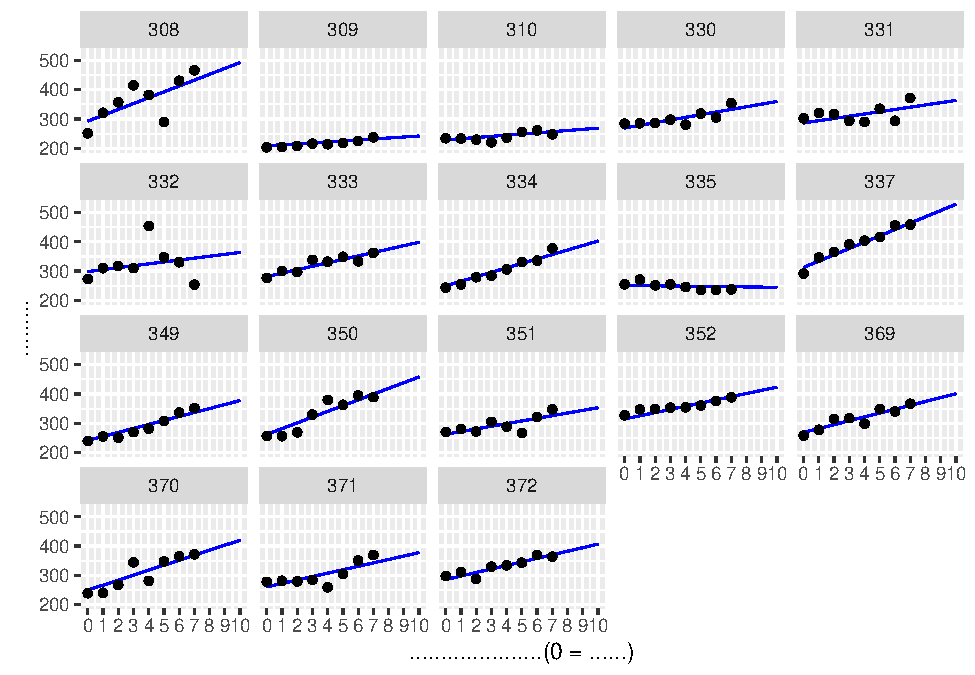
\includegraphics{05-介绍线性混合效应模型_files/figure-latex/extrap-plot-1.pdf}
\caption{\label{fig:extrap-plot}原始数据与外推模型}
\end{figure}

\hypertarget{ux591aux5c42app}{%
\section{多层app}\label{ux591aux5c42app}}

试试这个\href{https://rstudio-connect.psy.gla.ac.uk/multilevel}{多层网页app}以加深你对三种不同的多层建模方法的理解。

\hypertarget{ux5355ux968fux673aux56e0ux5b50ux7ebfux6027ux6df7ux5408ux6548ux5e94ux6a21ux578b}{%
\chapter{单随机因子线性混合效应模型}\label{ux5355ux968fux673aux56e0ux5b50ux7ebfux6027ux6df7ux5408ux6548ux5e94ux6a21ux578b}}

\hypertarget{ux4ec0ux4e48ux65f6ux5019ux4e3aux4ec0ux4e48ux4f60ux60f3ux7528ux7ebfux6027ux6df7ux5408ux6548ux5e94ux5efaux6a21ux53d6ux4ee3ux4f20ux7edfux7684ux5206ux6790}{%
\section{什么时候,为什么,你想用线性混合效应建模取代传统的分析?}\label{ux4ec0ux4e48ux65f6ux5019ux4e3aux4ec0ux4e48ux4f60ux60f3ux7528ux7ebfux6027ux6df7ux5408ux6548ux5e94ux5efaux6a21ux53d6ux4ee3ux4f20ux7edfux7684ux5206ux6790}}

我们已经反复强调了,心理学中的许多常用技术可以被视为一般线性模型的特例。这意味着可以用回归来替代这些技术。事实上,你可以使用以下四个函数之一来分析几乎任何在心理学中可以想象得到的数据集。

\begin{tabular}{l|l|l|l}
\hline
取样设计 & 数据类型 & 函数 & 描述\\
\hline
单层 & 连续、正态分布 & `base::lm()` & 简单线性模型\\
\hline
单层 & 计数或分类 & `base::glm()` & 广义线性模型\\
\hline
多层 & 连续、正态分布 & `lme4::lmer()` & 线性混合效应模型\\
\hline
多层 & 计数或分类 & `lme4::glmer()` & 广义线性混合效应模型\\
\hline
\end{tabular}

在本章结束时,你应该:

\begin{itemize}
\tightlist
\item
  理解如何使用回归来替代标准的ANOVA和t检验分析,适用于具有单一随机因子和连续因变量的数据;
\item
  能够进行模型比较(\texttt{anova()})以测试效果;
\item
  能够使用R回归公式语法来表达各种研究设计。
\end{itemize}

要决定使用四个回归函数中的哪一个,你需要回答两个问题。

\begin{enumerate}
\def\labelenumi{\arabic{enumi}.}
\tightlist
\item
  因变量代表哪种类型的数据,它是如何分布的?
\item
  数据是多层(multilevel)的还是单层(single level)的?
\end{enumerate}

这些函数的参数在所有四个版本中都非常相似。我们将在本课程后面部分学习如何分析计数和分类数据。现在,我们将重点放在连续数据上,但原理可以推广到其他类型的数据上。

以下是单层数据(没有重复测量的数据)的对比表:

\begin{tabular}{l|l|l}
\hline
检验类型 & 传统方法 & 回归方法\\
\hline
单样本t检验 & `t.test(y, mu = c)` & `lm(y \textasciitilde{} 1, offset = c)`\\
\hline
独立样本t检验 & `t.test(x, y)` & `lm(y \textasciitilde{} x)`\\
\hline
单因素方差分析 & `aov(y \textasciitilde{} x)` & `lm(y \textasciitilde{} x)`\\
\hline
多因素方差分析 & `aov(y \textasciitilde{} a * b)` & `lm(y \textasciitilde{} a * b)`\\
\hline
\end{tabular}

以上所有设计都是\emph{被试间}设计,没有重复测量(请注意,在多因子情况下,我们可能会将\texttt{a}和\texttt{b}替换为偏差编码的数值型预测变量,原因已在\href{交互效应.html}{交互章节}中讨论过)。

混合效应模型在处理多层数据时可以发挥作用。数据通常是多层的,原因有如下三种(多个原因可能同时适用):

\begin{enumerate}
\def\labelenumi{\arabic{enumi}.}
\tightlist
\item
  你有一个被试内因子,和/或
\item
  你有\textbf{假重复(pseudoreplications)},和/或
\item
  你有多个刺激项目(我们将在\href{交叉随机因子线性混合效应模型.html}{下一章}中讨论)。
\end{enumerate}

此时,回顾一下被试间因子与被试内因子的意义是个好主意。在\texttt{sleepstudy}数据中,你有被试内因子\texttt{Day}(实际上它更像是一个数值型变量,而不是一个因子;但它在每个被试内有多个变动值)。

\textbf{假重复}发生在同一条件下进行多次测量的情况下。例如,设想一个研究,你随机分配被试饮用两种饮料中的一种------酒精或水------然后进行一个简单的反应时任务,当灯光闪烁时尽快按下按钮。你可能会对每个被试进行多次反应时测量;假设你在100次试验中测量它。你有一个被试间因子(饮料类型)和每个被试的100次观测,对于每组的20个被试来说。一些新手在分析这些数据时常犯的错误是尝试进行t检验。\textbf{当你有假重复(或多个刺激)时,你不能直接使用传统的t检验}。你必须首先为每个被试计算均值,然后对\textbf{均值而不是原始数据}进行分析。虽然ANOVA的一些版本可以处理假重复,但使用线性混合效应模型可能更好,它可以更好地处理复杂的依赖结构(dependency structure)。

以下是多层数据的对比表:

\begin{tabular}{l|l|l}
\hline
检验类型 & 传统方法 & 回归方法\\
\hline
有假重复的单样本t检验 & 计算平均值并使用`t.test(x\_mean)` & <code>lmer(y \textasciitilde{} (1 | subject), offset = c)</code>\\
\hline
无假重复的配对样本t检验 & `t.test(x, y, paired = TRUE)` & <code>lmer(y \textasciitilde{} x + (1 | subject))</code>\\
\hline
有假重复的配对样本t检验 & 计算平均值并使用`t.test(x\_mean, y\_mean)` & <code>lmer(y \textasciitilde{} x + (1 + x | subject))</code>\\
\hline
无假重复的重复测量方差分析 & `aov(y \textasciitilde{} x + Error(subject))` & <code>lmer(y \textasciitilde{} x + (1 | subject))</code>\\
\hline
有假重复的重复测量方差分析 & `aov(y \textasciitilde{} x + Error(subject/x))` & <code>lmer(y \textasciitilde{} x + (1 + x | subject))</code>\\
\hline
无假重复的多因子方差分析,包含a和b & `aov(y \textasciitilde{} a * b + Error(subject))` & <code>lmer(y \textasciitilde{} a * b + (1 | subject))</code>\\
\hline
有假重复的多因子方差分析 & `aov(y \textasciitilde{} a * b + Error(subject/(a * b))` & <code>lmer(y \textasciitilde{} a * b + (1 + a * b | subject)</code>\\
\hline
\end{tabular}

广义线性模型/回归框架相比t检验和ANOVA的主要卖点之一就是灵活性。在上一章中,我们使用了\texttt{sleepstudy}数据,发现只有在线性混合效应模型框架才能妥善处理这些数据。尽管回归有许多优点,但如果你的数据是平衡的,且在不违反任何检验假设的情况下可以合理使用t检验或ANOVA,那么这样做是可取的;这些方法在心理学中有悠久的历史,并且更为广泛地被理解。

\hypertarget{ux793aux4f8bux591aux5c42ux6570ux636eux4e0aux7684ux72ecux7acbux6837ux672ctux68c0ux9a8c}{%
\section{\texorpdfstring{示例:多层数据上的独立样本\(t\)检验}{示例:多层数据上的独立样本t检验}}\label{ux793aux4f8bux591aux5c42ux6570ux636eux4e0aux7684ux72ecux7acbux6837ux672ctux68c0ux9a8c}}

让我们考虑一种情况,你在测试酒精摄入对简单反应时的影响(例如,灯亮后尽快按下按钮)。为了简化,假设你收集了14个被试的数据,这些被试被随机分配在两种干预后进行10次简单反应时试验:饮用一品脱酒精(处理条件)或饮用安慰剂饮料(安慰剂条件)。你在每组中有7名被试。请注意,实际研究中需要更多的被试。

这个\href{https://rstudio-connect.psy.gla.ac.uk/icc}{网页app}展示了这种研究的模拟数据。被试P01到P07属于安慰剂条件,而被试T01到T07属于处理条件。请停下并查看!

如果我们要对这些数据进行t检验,首先需要计算被试的均值,否则观测值不是独立的。你可以按如下方法进行操作。(如果你想运行下面的代码,可以从上面的网页app下载示例数据,并将其保存为\texttt{independent\_samples.csv})。

\begin{Shaded}
\begin{Highlighting}[]
\FunctionTok{library}\NormalTok{(tidyverse)}

\NormalTok{dat }\OtherTok{\textless{}{-}} \FunctionTok{read\_csv}\NormalTok{(}\StringTok{"data/independent\_samples.csv"}\NormalTok{, }\AttributeTok{col\_types =} \StringTok{"cci"}\NormalTok{)}

\NormalTok{subj\_means }\OtherTok{\textless{}{-}}\NormalTok{ dat }\SpecialCharTok{\%\textgreater{}\%}
  \FunctionTok{group\_by}\NormalTok{(subject, cond) }\SpecialCharTok{\%\textgreater{}\%}
  \FunctionTok{summarise}\NormalTok{(}\AttributeTok{mean\_rt =} \FunctionTok{mean}\NormalTok{(RT)) }\SpecialCharTok{\%\textgreater{}\%}
  \FunctionTok{ungroup}\NormalTok{()}

\NormalTok{subj\_means}
\end{Highlighting}
\end{Shaded}

\begin{verbatim}
## # A tibble: 14 x 3
##    subject cond  mean_rt
##    <chr>   <chr>   <dbl>
##  1 P01     P        354 
##  2 P02     P        384.
##  3 P03     P        391.
##  4 P04     P        404.
##  5 P05     P        421.
##  6 P06     P        392 
##  7 P07     P        400.
##  8 T08     T        430.
##  9 T09     T        432.
## 10 T10     T        410.
## 11 T11     T        455.
## 12 T12     T        450.
## 13 T13     T        418.
## 14 T14     T        489.
\end{verbatim}

然后可以使用\texttt{t.test()}进行\(t\)检验。

\begin{Shaded}
\begin{Highlighting}[]
\FunctionTok{t.test}\NormalTok{(mean\_rt }\SpecialCharTok{\textasciitilde{}}\NormalTok{ cond, subj\_means)}
\end{Highlighting}
\end{Shaded}

\begin{verbatim}
## 
##  Welch Two Sample t-test
## 
## data:  mean_rt by cond
## t = -3.7985, df = 11.32, p-value = 0.002807
## alternative hypothesis: true difference in means between group P and group T is not equal to 0
## 95 percent confidence interval:
##  -76.32580 -20.44563
## sample estimates:
## mean in group P mean in group T 
##        392.3143        440.7000
\end{verbatim}

虽然这样分析没有问题,但对数据进行聚合会丢失信息。我们可以在上面的网页app中看到,实际上存在两种不同的变异来源:简单反应时的逐试次变异(trial-by-trial variability,用\(\sigma\)表示)和被试相对于总体均值(\(\gamma_{00}\))的快慢的变异。被试\(s\)在试次\(t\)上的反应时(\(Y_{st}\))的数据生成过程如下所示。

\emph{第1层:}

\begin{equation}
Y_{st} = \beta_{0s} + \beta_{1} X_{s} + e_{st}
\end{equation}

\emph{第2层:}

\begin{equation}
\beta_{0s} = \gamma_{00} + S_{0s}
\end{equation}

\begin{equation}
\beta_{1} = \gamma_{10}
\end{equation}

\emph{方差成分:}

\begin{equation}
S_{0s} \sim N\left(0, {\tau_{00}}^2\right) 
\end{equation}

\begin{equation}
e_{st} \sim N\left(0, \sigma^2\right)
\end{equation}

在上面的方程中,\(X_s\)是一个数值型预测变量,用于编码被试\(s\)的条件;例如:0表示安慰剂,1表示处理。

相比于一个简单模型,多层方程显得有些繁琐,但是当我们遇到更复杂的设计时,熟悉一下多层格式是值得的;我们可以将第1层和第2层简化为

\begin{equation}
Y_{st} = \gamma_{00} + S_{0s} + \gamma_{10} X_s + e_{st},
\end{equation}

与上章节中的\texttt{sleepstudy}数据不同,现在的数据每个被试只有一个随机效应\(S_{0s}\),没有随机斜率。每个被试只出现在两个处理条件中的一个中,因此不可能估计安慰剂与酒精的效应在被试之间的变化情况。对于这些数据,我们拟合的混合效应模型,具有随机截距但没有随机斜率,被称为\textbf{随机截距模型(random intercepts model)}。

随机截距模型可以充分捕捉上述两种变异来源:参数\({\tau_{00}}^2\)中的总体平均反应时的被试间变异,以及参数\(\sigma^2\)中的逐试次变异。我们可以使用下面的公式计算个体差异在总变异中所占的比例。

\[ICC = \frac{{\tau_{00}}^2}{{\tau_{00}}^2 + \sigma^2}\]

这一数值被称为\textbf{组内相关系数(intra-class correlation coefficient)},告诉你数据中的聚类程度。它的范围从0到1,0表示所有变异都归因于残差变异,1表示所有变异都归因于被试间差异。

拟合随机截距模型的lmer语法是\texttt{lmer(RT\ \textasciitilde{}\ cond\ +\ (1\ \textbar{}\ subject),\ dat,\ REML=FALSE)}。首先让我们创建自己的数值型预测变量,以明确我们在使用虚拟编码。

\begin{Shaded}
\begin{Highlighting}[]
\NormalTok{dat2 }\OtherTok{\textless{}{-}}\NormalTok{ dat }\SpecialCharTok{\%\textgreater{}\%}
  \FunctionTok{mutate}\NormalTok{(}\AttributeTok{cond\_d =} \FunctionTok{if\_else}\NormalTok{(cond }\SpecialCharTok{==} \StringTok{"T"}\NormalTok{, 1L, 0L))}

\FunctionTok{distinct}\NormalTok{(dat2, cond, cond\_d)  }\DocumentationTok{\#\# 再次确认}
\end{Highlighting}
\end{Shaded}

\begin{verbatim}
## # A tibble: 2 x 2
##   cond  cond_d
##   <chr>  <int>
## 1 P          0
## 2 T          1
\end{verbatim}

现在估计模型。

\begin{Shaded}
\begin{Highlighting}[]
\FunctionTok{library}\NormalTok{(lme4)}

\NormalTok{mod }\OtherTok{\textless{}{-}} \FunctionTok{lmer}\NormalTok{(RT }\SpecialCharTok{\textasciitilde{}}\NormalTok{ cond\_d }\SpecialCharTok{+}\NormalTok{ (}\DecValTok{1} \SpecialCharTok{|}\NormalTok{ subject), dat2, }\AttributeTok{REML =} \ConstantTok{FALSE}\NormalTok{)}

\FunctionTok{summary}\NormalTok{(mod)}
\end{Highlighting}
\end{Shaded}

\begin{verbatim}
## Linear mixed model fit by maximum likelihood  ['lmerMod']
## Formula: RT ~ cond_d + (1 | subject)
##    Data: dat2
## 
##      AIC      BIC   logLik deviance df.resid 
##   1451.8   1463.5   -721.9   1443.8      136 
## 
## Scaled residuals: 
##      Min       1Q   Median       3Q      Max 
## -2.67117 -0.66677  0.01656  0.75361  2.58447 
## 
## Random effects:
##  Groups   Name        Variance Std.Dev.
##  subject  (Intercept)  329.3   18.15   
##  Residual             1574.7   39.68   
## Number of obs: 140, groups:  subject, 14
## 
## Fixed effects:
##             Estimate Std. Error t value
## (Intercept)  392.314      8.339  47.045
## cond_d        48.386     11.793   4.103
## 
## Correlation of Fixed Effects:
##        (Intr)
## cond_d -0.707
\end{verbatim}

使用上面app中的滑块并检查lmer输出面板,直到你了解输出结果如何映射到模型参数中。

\hypertarget{ux4ec0ux4e48ux65f6ux5019ux4f7fux7528ux968fux673aux622aux8dddux6a21ux578bux662fux5408ux9002ux7684}{%
\subsection{什么时候使用随机截距模型是合适的?}\label{ux4ec0ux4e48ux65f6ux5019ux4f7fux7528ux968fux673aux622aux8dddux6a21ux578bux662fux5408ux9002ux7684}}

当然,混合效应模型仅在你有多层数据时才合适。随机截距模型适用于任何单样本或具有假重复的组间数据(如果在这种情况下你没有假重复,那么你就没有多层数据,可以直接使用普通回归,例如\texttt{lm()})。

``仅随机截距''模型也适用于设计中有被试内因素的情况,但\textbf{只有当你没有假重复数据时}才合适;也就是说,它\textbf{只}适用于每个被试在被试内因素的每个水平上只有一个观测值的情况。如果每个被试在每个水平/单元上有多个观测值,那么你需要用随机斜率来丰富你的随机效应结构,在下一节会进行讲述。如果你有多个观测值的原因是每个被试对相同的刺激集合做出反应,那么你可能需要考虑一个对被试和刺激进行交叉随机效应的混合效应模型,在\href{交叉随机因子线性混合效应模型.html}{下一章}会进行讲述。

同样的逻辑也适用于有多个被试内因素的因子设计。在因子设计中,如果每个被试在由被试内因素相互组合形成的每个\textbf{单元}中只有一个观测值,那么随机截距模型是合适的。例如,如果\(A\)和\(B\)是2个两水平的被试内因素,你需要检查每个被试在\(A_1B_1\)、\(A_1B_2\)、\(A_2B_1\)和\(A_2B_2\)中是否只有1个观测值。如果有多个观测值,你将需要考虑在模型中加入随机斜率。

\hypertarget{ux7528ux56deux5f52ux8868ux8fbeux7814ux7a76ux8bbeux8ba1ux548cux8fdbux884cux68c0ux9a8c}{%
\section{用回归表达研究设计和进行检验}\label{ux7528ux56deux5f52ux8868ux8fbeux7814ux7a76ux8bbeux8ba1ux548cux8fdbux884cux68c0ux9a8c}}

为了在线性混合效应模型中重现所有的t检验/ANOVA风格的分析,你需要更好地理解两件事:(1)如何在回归公式中表达你的研究设计,以及(2)如何为你进行的任何检验获得p值。在线性混合效应方法中,后者并不是理所应当的,因为在许多情况下,\texttt{lme4::lmer()}的输出默认不会给出p值,这反映了存在多种获取p值的方法\citep{Luke_2017}。或者,你可能会为单个回归系数获得p值,但你想进行的检验是一个组合测试,需要同时测试多个参数。

首先,让我们仔细看看R和\textbf{\texttt{lme4}}中的回归公式语法。对于基于被试的随机效应的回归模型\(y = \beta_0 + \beta_1 x_1 + \beta_2 x_2 + \ldots + \beta_m x_m + e\),公式如下:

\texttt{y\ \textasciitilde{}\ 1\ +\ x1\ +\ x2\ +\ ...\ +\ xm\ +\ (1\ +\ x1\ +\ ...\ \textbar{}\ subject)}

残差项是隐含的,所以没有提及;仅列出预测变量。左边部分(波浪号\texttt{\textasciitilde{}}前面)指定响应变量,右侧是预测变量。括号中的项\texttt{(...\ \textbar{}\ ...)}特定于\textbf{\texttt{lme4}}。竖线\texttt{\textbar{}}的右侧指定一个变量名称(在本例中为\texttt{subject}),用于编码随机因子的水平。左侧指定你希望在这些水平上变化的回归系数。公式开头的\texttt{1}指定你需要一个截距,默认情况下已包括在内,因此可以省略。括号内的\texttt{1}指定一个\textbf{随机截距},这也是默认包含的;括号内提到的预测变量指定\textbf{随机斜率}。因此,你可以将上述公式等效写成:

\texttt{y\ \textasciitilde{}\ x1\ +\ x2\ +\ ...\ +\ xm\ +\ (x1\ +\ ...\ \textbar{}\ subject)}。

R公式中还有另一种重要的简写方式,我们已经在\protect\hyperlink{ux4ea4ux4e92ux6548ux5e94}{交互效应}章节中看到过,即被称为``星号语法''用于指定交互的\texttt{a\ *\ b}。如果你的设计中有两个因子\texttt{a}和\texttt{b},并且希望模型中包含所有主效应和交互效应,可以使用:

\texttt{y\ \textasciitilde{}\ a\ *\ b}

这等同于\texttt{y\ \textasciitilde{}\ a\ +\ b\ +\ a:b},其中\texttt{a}和\texttt{b}是编码A和B主效应的预测变量,\texttt{a:b}编码AB交互效应。使用星号语法指定交互比手动拼写它们要节省很多拼写(和错误)。这在下面的例子中更容易看出,该例子编码了一个包括因子A、B和C的2x2x2因子设计:

\texttt{y\ \textasciitilde{}\ a\ *\ b\ *\ c}

这等同于

\texttt{y\ \textasciitilde{}\ a\ +\ b\ +\ c\ +\ a:b\ +\ a:c\ +\ b:c\ +\ a:b:c}

其中\texttt{a:b}、\texttt{a:c}和\texttt{b:c}是双因子交互,\texttt{a:b:c}是三因子交互。你也可以在括号内的随机效应项中使用星号语法,例如:

\texttt{y\ \textasciitilde{}\ a\ *\ b\ *\ c\ +\ (a\ *\ b\ *\ c\ \textbar{}\ subject)}

等同于

\texttt{y\ \textasciitilde{}\ a\ +\ b\ +\ c\ +\ a:b\ +\ a:c\ +\ b:c\ +\ a:b:c\ +\ (a\ +\ b\ +\ c\ +\ a:b\ +\ a:c\ +\ b:c\ +\ a:b:c\ \textbar{}\ subject)}

尽管很复杂,但这种设计在心理学中并不罕见(例如,所有因子都在被试内,且每个条件有多个刺激)!

\hypertarget{ux6c34ux5e73ux4ee5ux4e0aux7684ux56e0ux5b50}{%
\subsection{2水平以上的因子}\label{ux6c34ux5e73ux4ee5ux4e0aux7684ux56e0ux5b50}}

如上所述,您可以使用公式\texttt{lm(y\ \textasciitilde{}\ x)}在回归中进行单因素ANOVA,对于单层数据,或者对于没有假重复的多层数据,使用公式\texttt{lmer(y\ \textasciitilde{}\ x\ +\ (1\ \textbar{}\ subject))}。在公式中,预测变量\texttt{x}应为\texttt{factor()}类型,R(默认情况下)会将其转换为\(k-1\)个虚拟编码的数值型预测变量(每个水平1个;有关信息,参见\protect\hyperlink{ux4ea4ux4e92ux6548ux5e94}{交互效应})。

自己编码数值预测变量通常是明智的,特别是在你的目标是进行ANOVA风格的主效应和交互效应检验的时候。这时如果你有变量是\texttt{factor}类型,可能会很困难。因此,对于一个名为\texttt{meal}(\texttt{breakfast},\texttt{lunch},\texttt{dinner})的3水平因子,你可以创建两个变量,\texttt{lunch\_v\_breakfast}和\texttt{dinner\_v\_breakfast},如下所示。

\begin{tabular}{l|r|r}
\hline
factor level & lunch\_v\_breakfast & dinner\_v\_breakfast\\
\hline
breakfast & -1/3 & -1/3\\
\hline
lunch & +2/3 & -1/3\\
\hline
dinner & -1/3 & +2/3\\
\hline
\end{tabular}

如果你的因变量是\texttt{calories},模型将会是:

\texttt{calories\ \textasciitilde{}\ lunch\_v\_breakfast\ +\ dinner\_v\_breakfast}。

但是如果你想要让\texttt{meal}与另一个两水平因素------\texttt{time\_of\_week}(分别编码为 -0.5 和 +0.5 的\texttt{weekday}和\texttt{weekend})进行交互,因为你认为每顿饭消耗的卡路里在这个变量的不同水平上会有所不同。那么你的模型将是:

\texttt{calories\ \textasciitilde{}\ (lunch\_v\_breakfast\ +\ dinner\_v\_breakfast)\ *\ time\_of\_week}。

\href{交互效应.html\#分类变量的编码方案}{包含交互效应是我们选择``偏差''编码方案的原因}。我们在与2水平变量相关的预测变量周围加上括号,以便每个预测变量都与\texttt{time\_of\_week}交互。上面的星形语法是以下形式的简写:

\texttt{calories\ \textasciitilde{}\ lunch\_v\_breakfast\ +\ dinner\_v\_breakfast\ +\ time\_of\_week\ +\ lunch\_v\_breakfast:time\_of\_week\ +\ dinner\_v\_breakfast:time\_of\_week}.

这是估计3x2因子设计参数的``回归方法''。

\hypertarget{ux591aux53c2ux6570ux68c0ux9a8c}{%
\subsection{多参数检验}\label{ux591aux53c2ux6570ux68c0ux9a8c}}

当你处理的设计中所有分类因子的水平都不超过两个时,与给定因子相关的回归系数检验将等同于ANOVA框架中的效应检验,前提是你使用\href{多元回归.html\#处理分类预测变量}{求和或偏差编码}。但是在上述示例中,我们有一个3x2设计,其中两个预测变量分别编码\texttt{meal}的主效应(\texttt{lunch\_v\_breakfast}和\texttt{dinner\_v\_breakfast})。让我们模拟一些数据并使用\texttt{aov()}运行一个单因素ANOVA,然后我们将使用回归函数\texttt{lm()}复制该分析(请注意,对于多层数据的混合效应模型,使用\texttt{lme4::lmer()}代替\texttt{base::lm()}也能得到相同的结果)。

\begin{Shaded}
\begin{Highlighting}[]
\DocumentationTok{\#\# 模拟一些数据}
\FunctionTok{set.seed}\NormalTok{(}\DecValTok{62}\NormalTok{)}
\NormalTok{meals }\OtherTok{\textless{}{-}} \FunctionTok{tibble}\NormalTok{(}\AttributeTok{meal =} \FunctionTok{factor}\NormalTok{(}\FunctionTok{rep}\NormalTok{(}\FunctionTok{c}\NormalTok{(}\StringTok{"breakfast"}\NormalTok{, }\StringTok{"lunch"}\NormalTok{, }\StringTok{"dinner"}\NormalTok{),}
                                  \AttributeTok{each =} \DecValTok{6}\NormalTok{)),}
                \AttributeTok{time\_of\_week =} \FunctionTok{factor}\NormalTok{(}\FunctionTok{rep}\NormalTok{(}\FunctionTok{rep}\NormalTok{(}\FunctionTok{c}\NormalTok{(}\StringTok{"weekday"}\NormalTok{, }\StringTok{"weekend"}\NormalTok{),}
                                              \AttributeTok{each =} \DecValTok{3}\NormalTok{), }\DecValTok{3}\NormalTok{)),}
                \AttributeTok{calories =} \FunctionTok{rnorm}\NormalTok{(}\DecValTok{18}\NormalTok{, }\DecValTok{450}\NormalTok{, }\DecValTok{50}\NormalTok{))}

\DocumentationTok{\#\# 使用求和编码代替默认的虚拟(处理)编码}
\FunctionTok{options}\NormalTok{(}\AttributeTok{contrasts =} \FunctionTok{c}\NormalTok{(}\AttributeTok{unordered =} \StringTok{"contr.sum"}\NormalTok{, }\AttributeTok{ordered =} \StringTok{"contr.poly"}\NormalTok{))}

\FunctionTok{aov}\NormalTok{(calories }\SpecialCharTok{\textasciitilde{}}\NormalTok{ meal }\SpecialCharTok{*}\NormalTok{ time\_of\_week, }\AttributeTok{data =}\NormalTok{ meals) }\SpecialCharTok{\%\textgreater{}\%}
  \FunctionTok{summary}\NormalTok{()}
\end{Highlighting}
\end{Shaded}

\begin{verbatim}
##                   Df Sum Sq Mean Sq F value Pr(>F)
## meal               2   2164    1082   0.380  0.692
## time_of_week       1   5084    5084   1.783  0.207
## meal:time_of_week  2   4767    2384   0.836  0.457
## Residuals         12  34209    2851
\end{verbatim}

我们得到3个\(F\)检验,每个主效应各1个(\texttt{meal}和\texttt{time\_of\_week}),交互效应1个。如果我们用\texttt{lm()}来拟合模型呢?

\begin{Shaded}
\begin{Highlighting}[]
\DocumentationTok{\#\# 添加我们自己的数值型变量}
\NormalTok{meals2 }\OtherTok{\textless{}{-}}\NormalTok{ meals }\SpecialCharTok{\%\textgreater{}\%}
  \FunctionTok{mutate}\NormalTok{(}\AttributeTok{lunch\_v\_breakfast =} \FunctionTok{if\_else}\NormalTok{(meal }\SpecialCharTok{==} \StringTok{"lunch"}\NormalTok{, }\DecValTok{2}\SpecialCharTok{/}\DecValTok{3}\NormalTok{, }\SpecialCharTok{{-}}\DecValTok{1}\SpecialCharTok{/}\DecValTok{3}\NormalTok{),}
         \AttributeTok{dinner\_v\_breakfast =} \FunctionTok{if\_else}\NormalTok{(meal }\SpecialCharTok{==} \StringTok{"dinner"}\NormalTok{, }\DecValTok{2}\SpecialCharTok{/}\DecValTok{3}\NormalTok{, }\SpecialCharTok{{-}}\DecValTok{1}\SpecialCharTok{/}\DecValTok{3}\NormalTok{),}
         \AttributeTok{time\_week =} \FunctionTok{if\_else}\NormalTok{(time\_of\_week }\SpecialCharTok{==} \StringTok{"weekend"}\NormalTok{, }\DecValTok{1}\SpecialCharTok{/}\DecValTok{2}\NormalTok{, }\SpecialCharTok{{-}}\DecValTok{1}\SpecialCharTok{/}\DecValTok{2}\NormalTok{))}

\DocumentationTok{\#\# 再此确认我们的编码}
\FunctionTok{distinct}\NormalTok{(meals2, meal, time\_of\_week,}
\NormalTok{         lunch\_v\_breakfast, dinner\_v\_breakfast, time\_week)}
\end{Highlighting}
\end{Shaded}

\begin{verbatim}
## # A tibble: 6 x 5
##   meal      time_of_week lunch_v_breakfast dinner_v_breakfast time_week
##   <fct>     <fct>                    <dbl>              <dbl>     <dbl>
## 1 breakfast weekday                 -0.333             -0.333      -0.5
## 2 breakfast weekend                 -0.333             -0.333       0.5
## 3 lunch     weekday                  0.667             -0.333      -0.5
## 4 lunch     weekend                  0.667             -0.333       0.5
## 5 dinner    weekday                 -0.333              0.667      -0.5
## 6 dinner    weekend                 -0.333              0.667       0.5
\end{verbatim}

\begin{Shaded}
\begin{Highlighting}[]
\DocumentationTok{\#\# 拟合回归模型}
\NormalTok{mod }\OtherTok{\textless{}{-}} \FunctionTok{lm}\NormalTok{(calories }\SpecialCharTok{\textasciitilde{}}\NormalTok{ (lunch\_v\_breakfast }\SpecialCharTok{+}\NormalTok{ dinner\_v\_breakfast) }\SpecialCharTok{*}
\NormalTok{            time\_week, }\AttributeTok{data =}\NormalTok{ meals2)}

\FunctionTok{summary}\NormalTok{(mod)}
\end{Highlighting}
\end{Shaded}

\begin{verbatim}
## 
## Call:
## lm(formula = calories ~ (lunch_v_breakfast + dinner_v_breakfast) * 
##     time_week, data = meals2)
## 
## Residuals:
##     Min      1Q  Median      3Q     Max 
## -68.522 -35.895  -4.063  42.061  73.081 
## 
## Coefficients:
##                              Estimate Std. Error t value Pr(>|t|)    
## (Intercept)                    451.15      12.58  35.848 1.42e-13 ***
## lunch_v_breakfast              -25.23      30.83  -0.818    0.429    
## dinner_v_breakfast             -20.59      30.83  -0.668    0.517    
## time_week                       33.61      25.17   1.335    0.207    
## lunch_v_breakfast:time_week    -58.31      61.65  -0.946    0.363    
## dinner_v_breakfast:time_week    17.93      61.65   0.291    0.776    
## ---
## Signif. codes:  0 '***' 0.001 '**' 0.01 '*' 0.05 '.' 0.1 ' ' 1
## 
## Residual standard error: 53.39 on 12 degrees of freedom
## Multiple R-squared:  0.2599, Adjusted R-squared:  -0.04843 
## F-statistic: 0.843 on 5 and 12 DF,  p-value: 0.5447
\end{verbatim}

好的,这个输出结果看起来非常不同!在这种情况下,如何执行类似ANOVA的检验呢?你已经得到了\texttt{lunch\_v\_breakfast}和\texttt{dinner\_v\_breakfast}的估计值,但如何将其转换为对\texttt{meal}主效应的单一检验呢?同样,你有两个交互项\texttt{lunch\_v\_breakfast:tow}和\texttt{dinner\_v\_breakfast:tow},如何将其转换为对交互效应的单一检验呢?

解决方案是使用模型比较进行\textbf{多参数检验},在R中由\texttt{anova()}函数实现。为了检验\texttt{meal}的主效应,你需要比较包含编码该因素的两个预测变量(\texttt{lunch\_v\_breakfast}和\texttt{dinner\_v\_breakfast})的模型与一个不包含这两个预测变量但其他部分相同的模型。你可以重新写个模型并排除这些项来重新拟合模型,或者使用\texttt{update()}函数并移除这些项(这是一种简写方法)。我们先写出来。

\begin{Shaded}
\begin{Highlighting}[]
\DocumentationTok{\#\# 拟合模型}
\NormalTok{mod\_main\_eff }\OtherTok{\textless{}{-}} \FunctionTok{lm}\NormalTok{(calories }\SpecialCharTok{\textasciitilde{}}\NormalTok{ time\_week }\SpecialCharTok{+}
\NormalTok{                     lunch\_v\_breakfast}\SpecialCharTok{:}\NormalTok{time\_week }\SpecialCharTok{+}\NormalTok{ dinner\_v\_breakfast}\SpecialCharTok{:}\NormalTok{time\_week,}
\NormalTok{                   meals2)}

\DocumentationTok{\#\# 比较模型}
\FunctionTok{anova}\NormalTok{(mod, mod\_main\_eff)}
\end{Highlighting}
\end{Shaded}

\begin{verbatim}
## Analysis of Variance Table
## 
## Model 1: calories ~ (lunch_v_breakfast + dinner_v_breakfast) * time_week
## Model 2: calories ~ time_week + lunch_v_breakfast:time_week + dinner_v_breakfast:time_week
##   Res.Df   RSS Df Sum of Sq      F Pr(>F)
## 1     12 34209                           
## 2     14 36373 -2   -2163.9 0.3795 0.6921
\end{verbatim}

好的,现在这里是使用简写方法\texttt{update()}函数的等效版本,它将你想要更新的模型作为第一个参数,然后使用特殊语法来进行你的更改。对于公式,我们使用\texttt{.\ \textasciitilde{}\ .\ -lunch\_v\_breakfast\ -dinner\_v\_breakfast\textasciitilde{}}。虽然这个公式看起来有些奇怪,但点\texttt{.}表示``在模型公式的这一侧(\texttt{\textasciitilde{}}左侧)保持原模型中的所有内容不变''。因此,公式\texttt{.\ \textasciitilde{}\ .}表示使用与原模型相同的公式;也就是说\texttt{update(mod,\ .\ \textasciitilde{}\ .)}将拟合与上述完全相同的模型。相比之下,\texttt{.\ \textasciitilde{}\ .\ -x\ -y}意味着``左侧保持不变(相同的因变量),但从右侧移除变量\texttt{x}和\texttt{y}''。

\begin{Shaded}
\begin{Highlighting}[]
\NormalTok{mod\_main\_eff2 }\OtherTok{\textless{}{-}} \FunctionTok{update}\NormalTok{(mod, . }\SpecialCharTok{\textasciitilde{}}\NormalTok{ . }\SpecialCharTok{{-}}\NormalTok{lunch\_v\_breakfast }\SpecialCharTok{{-}}\NormalTok{dinner\_v\_breakfast)}

\FunctionTok{anova}\NormalTok{(mod, mod\_main\_eff2)}
\end{Highlighting}
\end{Shaded}

\begin{verbatim}
## Analysis of Variance Table
## 
## Model 1: calories ~ (lunch_v_breakfast + dinner_v_breakfast) * time_week
## Model 2: calories ~ time_week + lunch_v_breakfast:time_week + dinner_v_breakfast:time_week
##   Res.Df   RSS Df Sum of Sq      F Pr(>F)
## 1     12 34209                           
## 2     14 36373 -2   -2163.9 0.3795 0.6921
\end{verbatim}

如你所见,这给出了和之前相同的结果。

如果你想检验\texttt{time\_of\_week}的主效应,去掉这个预测因子。

\begin{Shaded}
\begin{Highlighting}[]
\NormalTok{mod\_tow }\OtherTok{\textless{}{-}} \FunctionTok{update}\NormalTok{(mod, . }\SpecialCharTok{\textasciitilde{}}\NormalTok{ . }\SpecialCharTok{{-}}\NormalTok{time\_week)}

\FunctionTok{anova}\NormalTok{(mod, mod\_tow)}
\end{Highlighting}
\end{Shaded}

\begin{verbatim}
## Analysis of Variance Table
## 
## Model 1: calories ~ (lunch_v_breakfast + dinner_v_breakfast) * time_week
## Model 2: calories ~ lunch_v_breakfast + dinner_v_breakfast + lunch_v_breakfast:time_week + 
##     dinner_v_breakfast:time_week
##   Res.Df   RSS Df Sum of Sq      F Pr(>F)
## 1     12 34209                           
## 2     13 39294 -1   -5084.1 1.7834 0.2065
\end{verbatim}

试着弄清楚如何检验交互效应。

点击查看答案

\begin{Shaded}
\begin{Highlighting}[]
\NormalTok{mod\_interact }\OtherTok{\textless{}{-}} \FunctionTok{update}\NormalTok{(mod, . }\SpecialCharTok{\textasciitilde{}}\NormalTok{ . }\SpecialCharTok{{-}}\NormalTok{lunch\_v\_breakfast}\SpecialCharTok{:}\NormalTok{time\_week}
                       \SpecialCharTok{{-}}\NormalTok{dinner\_v\_breakfast}\SpecialCharTok{:}\NormalTok{time\_week)}

\FunctionTok{anova}\NormalTok{(mod, mod\_interact)}
\end{Highlighting}
\end{Shaded}

\begin{verbatim}
## Analysis of Variance Table
## 
## Model 1: calories ~ (lunch_v_breakfast + dinner_v_breakfast) * time_week
## Model 2: calories ~ lunch_v_breakfast + dinner_v_breakfast + time_week
##   Res.Df   RSS Df Sum of Sq      F Pr(>F)
## 1     12 34209                           
## 2     14 38977 -2   -4767.4 0.8362 0.4571
\end{verbatim}

我们使用\texttt{lm()}进行模型比较得到了与使用\texttt{aov()}完全相同的结果。尽管这涉及更多的步骤,但学习这种方法是值得的,因为它最终会让你有更多的灵活性。

\hypertarget{ux4ea4ux53c9ux968fux673aux56e0ux5b50ux7ebfux6027ux6df7ux5408ux6548ux5e94ux6a21ux578b}{%
\chapter{交叉随机因子线性混合效应模型}\label{ux4ea4ux53c9ux968fux673aux56e0ux5b50ux7ebfux6027ux6df7ux5408ux6548ux5e94ux6a21ux578b}}

\hypertarget{ux6982ux62ecux88abux8bd5ux548cux523aux6fc0ux7684ux7ec4ux5408}{%
\section{概括被试和刺激的组合}\label{ux6982ux62ecux88abux8bd5ux548cux523aux6fc0ux7684ux7ec4ux5408}}

心理学实验的一个常见目标是检验关于在特定类型的刺激下行为发生的主张(有时是关于该行为神经基础的结论)。这些刺激可能是单词、图像、声音、视频或故事。你可能想检验的主张的一些例子包括:

\begin{itemize}
\tightlist
\item
  在听第二语言的单词时,双语者是否会受到母语单词的干扰?
\item
  人们在心情好的时候和心情不好的时候对面孔的吸引力评分是否不同?
\item
  相对于更中性的图像,观看舒适的图像是否有助于减轻压力?
\item
  在阅读模糊描述目标个体的场景时,被潜意识启动后,人们是否更有可能对目标所属的社会群体做出假设?
\end{itemize}

关于所有这些主张需要注意的一点是,它们的形式都是:``当类型为X的个体遇到类型为Y的刺激时,我们的测量结果会发生什么变化'',其中X是从目标被试的总体中抽取的,Y是从目标刺激的总体中抽取的。换句话说,我们试图对涉及被试和刺激的采样单元\textbf{相遇}产生的特定类别的\textbf{事件}做出可推广的主张\citep{Barr_2017}。但就像我们不能从目标被试的总体中采样所有可能的被试一样,我们也不能从目标刺激的总体中采样所有可能的刺激。因此,在做推断时,我们需要考虑由\emph{两种}采样过程引入的估计不确定性\citep{Coleman_1964, Clark_1973, Judd_Westfall_Kenny_2012, yarkoni_2019}。线性混合效应模型通过允许我们的模型公式中有多个随机因子而特别容易做到这一点\citep{Baayen_Davidson_Bates_2008}。

这里有一个简单的例子,你感兴趣的是检验人们是否认为猫、狗或日落的图片看起来更舒适。你想对猫、狗和日落这类图片做出一般性陈述,而不是关于你碰巧采样的具体图片。假设你从Google图片中随机为每类选取4张图片(你绝对需要更多的图片才能做出一般性陈述,但我们选择少量图片以使示例简单)。因此,你的刺激表可能如下所示:

\begin{tabular}{r|l|l}
\hline
stimulus\_id & category & file\\
\hline
1 & cat & cat1.jpg\\
\hline
2 & cat & cat2.jpg\\
\hline
3 & cat & cat3.jpg\\
\hline
4 & cat & cat4.jpg\\
\hline
5 & dog & dog1.jpg\\
\hline
6 & dog & dog2.jpg\\
\hline
7 & dog & dog3.jpg\\
\hline
8 & dog & dog4.jpg\\
\hline
9 & sunset & sunset1.jpg\\
\hline
10 & sunset & sunset2.jpg\\
\hline
11 & sunset & sunset3.jpg\\
\hline
12 & sunset & sunset4.jpg\\
\hline
\end{tabular}

然后你抽取了4个被试来进行舒适度评分。再次强调,4个被试对于真实研究来说太少了,但为了便于解释我们保持数据量很小。

\begin{tabular}{r|r|l}
\hline
subject\_id & age & date\\
\hline
1 & 65 & 2020-05-08\\
\hline
2 & 58 & 2020-05-10\\
\hline
3 & 57 & 2020-05-19\\
\hline
4 & 36 & 2020-05-28\\
\hline
\end{tabular}

现在,因为每个受试者对每张图片都进行了``舒适度''评分,所以你会有一个完整的数据集,包含所有的\texttt{subject\_id}和\texttt{stimulus\_id}组合。这就是我们所说的``交叉随机因子''。你可以使用\texttt{tidyr}(加载\texttt{tidyverse}时会一起加载)中的\texttt{crossing()}函数来创建包含所有这些组合的表。

\begin{Shaded}
\begin{Highlighting}[]
\FunctionTok{crossing}\NormalTok{(subjects }\SpecialCharTok{\%\textgreater{}\%} \FunctionTok{select}\NormalTok{(subject\_id),}
\NormalTok{         stimuli }\SpecialCharTok{\%\textgreater{}\%} \FunctionTok{select}\NormalTok{(}\SpecialCharTok{{-}}\NormalTok{category)) }
\end{Highlighting}
\end{Shaded}

\begin{tabular}{r|r|l}
\hline
subject\_id & stimulus\_id & file\\
\hline
1 & 1 & cat1.jpg\\
\hline
1 & 2 & cat2.jpg\\
\hline
1 & 3 & cat3.jpg\\
\hline
1 & 4 & cat4.jpg\\
\hline
1 & 5 & dog1.jpg\\
\hline
1 & 6 & dog2.jpg\\
\hline
1 & 7 & dog3.jpg\\
\hline
1 & 8 & dog4.jpg\\
\hline
1 & 9 & sunset1.jpg\\
\hline
1 & 10 & sunset2.jpg\\
\hline
1 & 11 & sunset3.jpg\\
\hline
1 & 12 & sunset4.jpg\\
\hline
2 & 1 & cat1.jpg\\
\hline
2 & 2 & cat2.jpg\\
\hline
2 & 3 & cat3.jpg\\
\hline
2 & 4 & cat4.jpg\\
\hline
2 & 5 & dog1.jpg\\
\hline
2 & 6 & dog2.jpg\\
\hline
2 & 7 & dog3.jpg\\
\hline
2 & 8 & dog4.jpg\\
\hline
2 & 9 & sunset1.jpg\\
\hline
2 & 10 & sunset2.jpg\\
\hline
2 & 11 & sunset3.jpg\\
\hline
2 & 12 & sunset4.jpg\\
\hline
3 & 1 & cat1.jpg\\
\hline
3 & 2 & cat2.jpg\\
\hline
3 & 3 & cat3.jpg\\
\hline
3 & 4 & cat4.jpg\\
\hline
3 & 5 & dog1.jpg\\
\hline
3 & 6 & dog2.jpg\\
\hline
3 & 7 & dog3.jpg\\
\hline
3 & 8 & dog4.jpg\\
\hline
3 & 9 & sunset1.jpg\\
\hline
3 & 10 & sunset2.jpg\\
\hline
3 & 11 & sunset3.jpg\\
\hline
3 & 12 & sunset4.jpg\\
\hline
4 & 1 & cat1.jpg\\
\hline
4 & 2 & cat2.jpg\\
\hline
4 & 3 & cat3.jpg\\
\hline
4 & 4 & cat4.jpg\\
\hline
4 & 5 & dog1.jpg\\
\hline
4 & 6 & dog2.jpg\\
\hline
4 & 7 & dog3.jpg\\
\hline
4 & 8 & dog4.jpg\\
\hline
4 & 9 & sunset1.jpg\\
\hline
4 & 10 & sunset2.jpg\\
\hline
4 & 11 & sunset3.jpg\\
\hline
4 & 12 & sunset4.jpg\\
\hline
\end{tabular}

因为4个被试对12个刺激做出反应,所以结果表将有48行。

\hypertarget{lme4ux8bedux6cd5ux7528ux4e8eux4ea4ux53c9ux968fux673aux56e0ux5b50}{%
\section{lme4语法用于交叉随机因子}\label{lme4ux8bedux6cd5ux7528ux4e8eux4ea4ux53c9ux968fux673aux56e0ux5b50}}

如何分析这样的数据呢?回忆上一个章节中提到的,在lme4中,表示被试水平上的随机截距和预测变量\texttt{x}的随机斜率的模型的公式语法为\texttt{y\ \textasciitilde{}\ x\ +\ (1\ +\ x\ \textbar{}\ subject\_id)},其中用包含在括号中的竖线\texttt{\textbar{}}部分进行了随机效应的指定。竖线右侧的变量\texttt{subject\_id}指定了随机因子的水平。括号中竖线左侧的公式\texttt{1\ +\ x}指定了与该因子相关的随机效应,在这种情况下是随机截距和\texttt{x}的随机斜率。最好将这个括号中的部分\texttt{(1\ +\ x\ \textbar{}\ subject\_id)}理解为\textbf{对\texttt{lme4::lmer()}关于如何构建协方差矩阵以捕捉由随机因子被试引入的方差的指示}。到目前为止,你应该意识到,这个指示将指示一个二维协方差矩阵的估计,一个维度是截距方差,一个是斜率方差。

但我们并不仅局限于估计被试的随机效应;我们还可以通过简单地在公式中添加另一个项来指定刺激的随机效应。例如:

\texttt{y\ \textasciitilde{}\ x\ +\ (1\ +\ x\ \textbar{}\ subject\_id)\ +\ (1\ +\ x\ \textbar{}\ stimulus\_id)}。

这个公式通过\texttt{x}对\texttt{y}进行了回归,包含了被试水平上的随机截距和斜率的随机效应和刺激水平上的随机截距和斜率的随机效应。这样,拟合的模型将捕捉到我们估计中的两种不确定性来源------由被试抽样引入的不确定性以及由(刺激)项目抽样引入的不确定性。我们现在估计的是\textbf{两个独立的协方差矩阵},一个用于被试,一个用于(刺激)项目。在上述例子中,这两个矩阵都将具有相同的2x2结构,但情况未必总是如此。我们可以通过改变每个竖线\texttt{\textbar{}}符号左侧的公式灵活地更改随机效应结构。例如,如果我们有另一个预测变量\texttt{w},我们可以有:

\texttt{y\ \textasciitilde{}\ x\ +\ (x\ \textbar{}\ subject\_id)\ +\ (x\ +\ w\ \textbar{}\ stimulus\_id)}

这将为被试估计相同的2x2矩阵,但(刺激)项目的协方差矩阵现在是一个3x3矩阵(截距、\texttt{x}的斜率和 \texttt{w}的斜率)。虽然这提供了很大的灵活性,但随着随机效应结构变得更加复杂,估计过程变得更加困难,并且不太可能收敛得到结果。

\hypertarget{ux6307ux5b9aux968fux673aux6548ux5e94}{%
\section{指定随机效应}\label{ux6307ux5b9aux968fux673aux6548ux5e94}}

随机效应结构的选择并不是随着线性混合效应模型而出现的新问题。在使用t检验和ANOVA的传统方法中,当你选择使用何种流程时,你隐含地选择了随机效应结构。如上一章所讨论的,如果你选择配对样本t检验而不是独立样本t检验,这相当于选择拟合\texttt{lme4::lmer(y\ \textasciitilde{}\ x\ +\ (1\ \textbar{}\ subject))}而不是\texttt{lm(y\ \textasciitilde{}\ x)}。同样地,你可以将混合模型ANOVA运行为\texttt{aov(y\ \textasciitilde{}\ x\ +\ Error(subject\_id))},这相当于随机截距模型,或者\texttt{aov(y\ \textasciitilde{}\ x\ +\ Error(x\ /\ subject\_id))},这相当于随机斜率模型。心理学中进行验证性分析(confirmatory analyses)的传统是使用\textbf{研究设计所证明的最大随机效应结构}。所以,如果你有一个带有假重复的单因素数据,你会使用\texttt{aov(y\ \textasciitilde{}\ x\ +\ Error(x\ /\ subject\_id))}而不是\texttt{aov(y\ \textasciitilde{}\ x\ +\ Error(subject\_id))}。类似地,如果你使用线性混合效应模型来分析具有假重复的数据,你应该使用\texttt{lme4::lmer(y\ \textasciitilde{}\ x\ +\ (1\ +\ x\ \textbar{}\ subject\_id))}而不是\texttt{lme4::lmer(y\ \textasciitilde{}\ x\ +\ (1\ \textbar{}\ subject\_id))}。换句话说,你应该考虑由重复抽样相同被试或刺激引入的所有非独立性来源。这种方法被称为\textbf{最大随机效应法(maximal random effects approach)}或\textbf{设计驱动法(design-driven approach)}来指定随机效应结构\citep{Barr_et_al_2013}。未能考虑到设计引入的依赖性可能会导致标准差过小,进而导致p值小于实际值,从而提高假阳性概率(I类错误)。在某些情况下,这可能导致效力降低,从而提高假阴性概率(II类错误)。因此,进行分析时必须密切注意随机效应结构。

线性混合效应模型几乎不可避免地包含所有设计中随机因子的随机截距。因此,如果你的随机因子是由\texttt{subject\_id}和\texttt{stimulus\_id}标识的被试和刺激,那么至少你的模型语法将包含\texttt{(1\ \textbar{}\ subject\_id)\ +\ (1\ \textbar{}\ stimulus\_id)}。但你会在模型中有各种预测变量,因此关键问题是:我应该允许哪些预测变量在什么抽样单位上变化?例如,如果你的模型的固定效应部分是一个2x2因子设计,因子A和B,\texttt{y\ \textasciitilde{}\ a\ *\ b\ +\ ...},你可能会有各种随机效应结构,包括(但不限于):

\begin{enumerate}
\def\labelenumi{\arabic{enumi}.}
\tightlist
\item
  仅随机截距:\texttt{y\ \textasciitilde{}\ a\ *\ b\ +\ (1\ \textbar{}\ subject\_id)\ +\ (1\ \textbar{}\ stimulus\_id)}
\item
  被试水平上的a随机截距和(刺激)项目水平上的随机截距:\texttt{y\ \textasciitilde{}\ a\ *\ b\ +\ (a\ \textbar{}\ subject\_id)\ +\ (1\ \textbar{}\ stimulus\_id)}
\item
  被试水平上的a和b的随机截距和斜率及其交互效应,(刺激)项目水平上的随机截距:\texttt{y\ \textasciitilde{}\ a\ *\ b\ +\ (a\ *\ b\ \textbar{}\ subject\_id)\ +\ (1\ \textbar{}\ stimulus\_id)}
\item
  被试水平上的a和b的随机截距和斜率及其交互效应,(刺激)项目水平上的a和b的随机截距和斜率及其交互效应:\texttt{y\ \textasciitilde{}\ a\ *\ b\ +\ (a\ *\ b\ \textbar{}\ subject\_id)\ +\ (a\ *\ b\ \textbar{}\ stimulus\_id)}。
\end{enumerate}

有一点需要明确:

``由设计证明的最大随机效应结构''与``最大可能的随机效应结构''不同;也就是说,它并不意味着自动将所有预测变量的所有随机斜率放入所有随机因子中。你必须遵循下一部分中的随机效应指南,以决定是否应包含某个随机斜率。

一些作者建议采用``数据驱动''的随机效应结构替代设计驱动的随机效应结构,建议研究者仅在数据进一步证明的情况下才包含设计所证明的随机斜率\citep{Matuschek_et_al_2017}。例如,你可以使用虚无假设检验来确定是否包括一个被试水平上的\texttt{x}随机斜率显著提高了模型拟合,只有在显著提高时才包含该效应。虽然当随机斜率非常小时,这可能会在理论意义上提高检验的效力,但也会增加未知的假阳性风险,因此在检验的情景中是否应该采用这种方法是值得怀疑的。所以,我们不推荐基于数据的方法。

\hypertarget{ux4e3aux5206ux7c7bux56e0ux5b50ux9009ux62e9ux968fux673aux6548ux5e94ux7684ux89c4ux5219}{%
\subsection{为分类因子选择随机效应的规则}\label{ux4e3aux5206ux7c7bux56e0ux5b50ux9009ux62e9ux968fux673aux6548ux5e94ux7684ux89c4ux5219}}

线性混合效应模型的随机效应结构------即关于哪些效应在什么抽样单位上变化的假设------对于确保你的参数反映抽样引入的不确定性至关重要\citep{Barr_et_al_2013}。首先,请注意我们专注于代表\textbf{设计变量(design variable)}的预测变量,这些变量具有理论意义,并且你将对其进行推断检验。如果你有代表\textbf{控制变量(control variable)}的预测变量,而你不打算对其进行统计检验,那么通常不需要随机斜率。

以下规则源自 \citet{Barr_et_al_2013} 和 \citet{Barr_2013} 。如果你想了解这些指南的更多信息,请参考这些论文。请记住,只有当你有重复测量数据时,你才能使用混合效应模型,这可能是由于假重复和/或存在被试内(或刺激内)因子。在交叉随机因子的情况下,你不可避免地会有假重复------由于多个被试的多个刺激,每个被试的多个观测值,以及多个被试的每个刺激的多个观测值。确定随机效应结构的关键是弄清楚哪些因子是被试内或刺激内,以及设计中的假重复位于何处。你对被试使用一次规则以确定公式\texttt{(1\ +\ ...\ \textbar{}\ subject\_id)}部分的形式,并对刺激使用一次规则以确定公式\texttt{(1\ +\ ...\ \textbar{}\ stimulus\_id)}部分的形式。以下规则中的``单位''或``抽样单位''一词,根据需要替换为``被试''或``刺激''。

以下是规则:

\begin{enumerate}
\def\labelenumi{\arabic{enumi}.}
\tightlist
\item
  如果对抽样单位进行了重复测量,则需要该随机因子的随机截距:\texttt{(1\ \textbar{}\ unit\_id)};
\item
  如果一个因子\texttt{x}是单位间的,则不需要该因子的随机斜率;
\item
  确定所考虑的单位的被试内因子的最高阶交互效应。如果在这些组合定义的每个单元内有假重复(即每个单元的多个观测值),那么对于该单位,你将需要该交互效应的斜率以及所有低阶效应的斜率。如果没有假重复,则不需要任何随机斜率。
\end{enumerate}

前两条规则很简单,但第三条需要一些解释。首先问自己:我们怎么知道某个因子是单位间还是单位内的?

一个简单的方法是使用\texttt{dplyr::count()}函数(加载tidyverse时同时加载),它会提供频率计数。假设你对因子A是否在被试内还是被试者间感兴趣,对下面虚拟的2x2x2因子数据\texttt{abc\_data},其中 \(A\)、\(B\)和\(C\)是你的设计因子。

\begin{Shaded}
\begin{Highlighting}[]
\FunctionTok{library}\NormalTok{(tidyverse)}

\DocumentationTok{\#\# 运行代码创建"abc\_data"表}
\NormalTok{abc\_subj }\OtherTok{\textless{}{-}} \FunctionTok{tibble}\NormalTok{(}\AttributeTok{subject\_id =} \DecValTok{1}\SpecialCharTok{:}\DecValTok{4}\NormalTok{,}
                   \AttributeTok{B =} \FunctionTok{rep}\NormalTok{(}\FunctionTok{c}\NormalTok{(}\StringTok{"B1"}\NormalTok{, }\StringTok{"B2"}\NormalTok{), }\AttributeTok{times =} \DecValTok{2}\NormalTok{))}

\NormalTok{abc\_item  }\OtherTok{\textless{}{-}} \FunctionTok{tibble}\NormalTok{(}\AttributeTok{stimulus\_id =} \DecValTok{1}\SpecialCharTok{:}\DecValTok{4}\NormalTok{,}
                    \AttributeTok{A =} \FunctionTok{rep}\NormalTok{(}\FunctionTok{c}\NormalTok{(}\StringTok{"A1"}\NormalTok{, }\StringTok{"A2"}\NormalTok{), }\AttributeTok{each =} \DecValTok{2}\NormalTok{),}
                    \AttributeTok{C =} \FunctionTok{rep}\NormalTok{(}\FunctionTok{c}\NormalTok{(}\StringTok{"C1"}\NormalTok{, }\StringTok{"C2"}\NormalTok{), }\AttributeTok{times =} \DecValTok{2}\NormalTok{))}

\NormalTok{abc\_data }\OtherTok{\textless{}{-}} \FunctionTok{crossing}\NormalTok{(abc\_subj, abc\_item) }\SpecialCharTok{\%\textgreater{}\%}
  \FunctionTok{select}\NormalTok{(subject\_id, stimulus\_id, }\FunctionTok{everything}\NormalTok{())}
\end{Highlighting}
\end{Shaded}

查看\(A\)是被试内还是被试间,使用:

\begin{Shaded}
\begin{Highlighting}[]
\NormalTok{abc\_data }\SpecialCharTok{\%\textgreater{}\%}
  \FunctionTok{count}\NormalTok{(subject\_id, A)}
\end{Highlighting}
\end{Shaded}

\begin{verbatim}
## # A tibble: 8 x 3
##   subject_id A         n
##        <int> <chr> <int>
## 1          1 A1        2
## 2          1 A2        2
## 3          2 A1        2
## 4          2 A2        2
## 5          3 A1        2
## 6          3 A2        2
## 7          4 A1        2
## 8          4 A2        2
\end{verbatim}

在结果表中,你可以看到每个被试都接受了\(A\)的所有水平,说明这是个被试内因子。那么对于\(B\)和\(C\)呢?

\begin{Shaded}
\begin{Highlighting}[]
\NormalTok{abc\_data }\SpecialCharTok{\%\textgreater{}\%}
  \FunctionTok{count}\NormalTok{(subject\_id, B)}
\end{Highlighting}
\end{Shaded}

\begin{verbatim}
## # A tibble: 4 x 3
##   subject_id B         n
##        <int> <chr> <int>
## 1          1 B1        4
## 2          2 B2        4
## 3          3 B1        4
## 4          4 B2        4
\end{verbatim}

\begin{Shaded}
\begin{Highlighting}[]
\NormalTok{abc\_data }\SpecialCharTok{\%\textgreater{}\%}
  \FunctionTok{count}\NormalTok{(subject\_id, C)}
\end{Highlighting}
\end{Shaded}

\begin{verbatim}
## # A tibble: 8 x 3
##   subject_id C         n
##        <int> <chr> <int>
## 1          1 C1        2
## 2          1 C2        2
## 3          2 C1        2
## 4          2 C2        2
## 5          3 C1        2
## 6          3 C2        2
## 7          4 C1        2
## 8          4 C2        2
\end{verbatim}

\(B\)是被试间(每个被试只接受1个水平),\(C\)是被试内(每个被试接受所有水平)。

\emph{练习}

回答关于\texttt{abc\_data}的问题。

\begin{itemize}
\item
  因子\(A\)的水平是在刺激间还是刺激内?
\item
  \begin{enumerate}
  \def\labelenumi{(\Alph{enumi})}
  \tightlist
  \item
    between\\
  \end{enumerate}
\item
  \begin{enumerate}
  \def\labelenumi{(\Alph{enumi})}
  \setcounter{enumi}{1}
  \tightlist
  \item
    within
  \end{enumerate}
\end{itemize}

答案

\begin{Shaded}
\begin{Highlighting}[]
\NormalTok{abc\_data }\SpecialCharTok{\%\textgreater{}\%}
  \FunctionTok{count}\NormalTok{(stimulus\_id, A)}
\end{Highlighting}
\end{Shaded}

\begin{verbatim}
## # A tibble: 4 x 3
##   stimulus_id A         n
##         <int> <chr> <int>
## 1           1 A1        4
## 2           2 A1        4
## 3           3 A2        4
## 4           4 A2        4
\end{verbatim}

\begin{Shaded}
\begin{Highlighting}[]
\CommentTok{\# between}
\end{Highlighting}
\end{Shaded}

\begin{itemize}
\item
  因子\(B\)的水平是在刺激间还是刺激内?
\item
  \begin{enumerate}
  \def\labelenumi{(\Alph{enumi})}
  \tightlist
  \item
    between\\
  \end{enumerate}
\item
  \begin{enumerate}
  \def\labelenumi{(\Alph{enumi})}
  \setcounter{enumi}{1}
  \tightlist
  \item
    within
  \end{enumerate}
\end{itemize}

答案

\begin{Shaded}
\begin{Highlighting}[]
\NormalTok{abc\_data }\SpecialCharTok{\%\textgreater{}\%}
  \FunctionTok{count}\NormalTok{(stimulus\_id, B)}
\end{Highlighting}
\end{Shaded}

\begin{verbatim}
## # A tibble: 8 x 3
##   stimulus_id B         n
##         <int> <chr> <int>
## 1           1 B1        2
## 2           1 B2        2
## 3           2 B1        2
## 4           2 B2        2
## 5           3 B1        2
## 6           3 B2        2
## 7           4 B1        2
## 8           4 B2        2
\end{verbatim}

\begin{Shaded}
\begin{Highlighting}[]
\CommentTok{\# within}
\end{Highlighting}
\end{Shaded}

\begin{itemize}
\item
  因子\(C\)的水平是在刺激间还是刺激内?
\item
  \begin{enumerate}
  \def\labelenumi{(\Alph{enumi})}
  \tightlist
  \item
    between\\
  \end{enumerate}
\item
  \begin{enumerate}
  \def\labelenumi{(\Alph{enumi})}
  \setcounter{enumi}{1}
  \tightlist
  \item
    within
  \end{enumerate}
\end{itemize}

答案

\begin{Shaded}
\begin{Highlighting}[]
\NormalTok{abc\_data }\SpecialCharTok{\%\textgreater{}\%}
  \FunctionTok{count}\NormalTok{(stimulus\_id, C)}
\end{Highlighting}
\end{Shaded}

\begin{verbatim}
## # A tibble: 4 x 3
##   stimulus_id C         n
##         <int> <chr> <int>
## 1           1 C1        4
## 2           2 C2        4
## 3           3 C1        4
## 4           4 C2        4
\end{verbatim}

\begin{Shaded}
\begin{Highlighting}[]
\CommentTok{\# between}
\end{Highlighting}
\end{Shaded}

好的,我们已经确定了哪些因子是被试内和哪些被试间,以及哪些因子是刺激内和哪些刺激间。

第二条规则告诉我们,如果一个因子是单位间的,你不需要该因子的随机斜率。事实上,无法估计单位间因子的随机斜率。如果你考虑到随机斜率捕捉效应在单位之间的变化,那么只有当你在该因子的所有水平上测量了你的响应变量时,才能估计出这种变化。例如,如果你有一个名为处理组(实验组、对照组)的2水平因子,除非某个被试经历了该因子的两个水平(即它必须是被试内的),否则无法估计``治疗''对该被试的效应。

我们现在如何应用第三条规则来确定我们对单位内因子需要哪些随机斜率呢?

考虑到\(A\)和\(C\)是被试内的,\(B\)是被试间的。所以被试内因子的最高阶交互作用是\(AC\)。如果我们对每个被试在每个\(AC\)组合中有假重复,那么我们将需要\(AC\)交互效应的随机斜率以及主效应\(A\)和\(C\)的随机斜率。我们如何确定这一点呢?

\begin{Shaded}
\begin{Highlighting}[]
\NormalTok{abc\_data }\SpecialCharTok{\%\textgreater{}\%}
  \FunctionTok{count}\NormalTok{(subject\_id, A, C)}
\end{Highlighting}
\end{Shaded}

\begin{verbatim}
## # A tibble: 16 x 4
##    subject_id A     C         n
##         <int> <chr> <chr> <int>
##  1          1 A1    C1        1
##  2          1 A1    C2        1
##  3          1 A2    C1        1
##  4          1 A2    C2        1
##  5          2 A1    C1        1
##  6          2 A1    C2        1
##  7          2 A2    C1        1
##  8          2 A2    C2        1
##  9          3 A1    C1        1
## 10          3 A1    C2        1
## 11          3 A2    C1        1
## 12          3 A2    C2        1
## 13          4 A1    C1        1
## 14          4 A1    C2        1
## 15          4 A2    C1        1
## 16          4 A2    C2        1
\end{verbatim}

这向我们展示了对于每个\(AC\)组合,只有\emph{1}个观测值,因此我们不需要\(AC\)的随机斜率,也不需要\(A\)或\(C\)的随机斜率。被试水平上的随机效应公式就是\texttt{(1\ \textbar{}\ subject\_id)}。

刺激水平上的随机因子需要哪些随机斜率?

答案

你有1个刺激内因子\(B\),它进行了假重复。

\begin{Shaded}
\begin{Highlighting}[]
\NormalTok{abc\_data }\SpecialCharTok{\%\textgreater{}\%}
  \FunctionTok{count}\NormalTok{(stimulus\_id, B)}
\end{Highlighting}
\end{Shaded}

\begin{verbatim}
## # A tibble: 8 x 3
##   stimulus_id B         n
##         <int> <chr> <int>
## 1           1 B1        2
## 2           1 B2        2
## 3           2 B1        2
## 4           2 B2        2
## 5           3 B1        2
## 6           3 B2        2
## 7           4 B1        2
## 8           4 B2        2
\end{verbatim}

因此对于刺激的公式是\texttt{(B\ \textbar{}\ stimulus\_id)}, 完整的\texttt{lme4}公式是:

\texttt{y\ \textasciitilde{}\ A\ *\ B\ *\ C\ +\ (1\ \textbar{}\ subject\_id)\ +\ (B\ \textbar{}\ stimulus\_id)}.

\hypertarget{ux6392ux9664ux4e0dux6536ux655bux548cux7578ux5f62ux62dfux5408singular-fit}{%
\subsection{排除不收敛和``畸形拟合(singular fit)''}\label{ux6392ux9664ux4e0dux6536ux655bux548cux7578ux5f62ux62dfux5408singular-fit}}

当你试图拟合具有最大随机效应的模型时,可能会遇到几个不同的问题。回想一下,线性混合效应模型的估计算法是\emph{迭代(iterative)}------即拟合算法以逐步的方式搜索使数据最合适的参数值。有时它会一直搜索但找不到,这种情况下,你会收到``收敛警告''。当这种情况发生时,信任未收敛模型的任何估计值都不是一个好主意,你需要简化模型结构然后重试。

另一种情况是你会收到关于``畸形拟合''的信息。当估计过程包含一个或多个随机因子产生的方差-协方差矩阵有(1)完全或近乎完全(1.00,-1.00)的正或负相关,(2)一个或多个方差接近于0,或(3)两者兼有时,会出现这种信息。可能可以忽略此信息,但也有理由简化模型结构直到信息消失。

如何简化模型以处理收敛问题或畸形拟合信息呢?这需要小心操作。我建议以下策略:

\begin{enumerate}
\def\labelenumi{\arabic{enumi}.}
\tightlist
\item
  将所有协方差参数约束为0。这可以使用双竖线\texttt{\textbar{}\textbar{}}语法来完成,例如,将\texttt{(a\ *\ b\ \textbar{}\ subject)}更改为\texttt{(a\ *\ b\ \textbar{}\textbar{}\ subject)}。如果仍然遇到估计问题,那么:
\item
  检查非收敛或畸形模型的参数估计值。是否有任何斜率变量为0或接近于0?删除这些变量并重新拟合模型,重复此步骤直到收敛警告/畸形拟合信息消失。
\end{enumerate}

有关收敛问题的更多技术细节以及如何处理,参见\texttt{?lme4::convergence}和\texttt{?lme4::isSingular}。

注:推荐阅读\href{https://github.com/usplos/Eye-movement-related/blob/master/Linear\%20mixed\%20model\%20(Hierarchical\%20linear\%20model)\%20using\%20R\%20and\%20JAMOVI.md}{混合线性模型的实现}加深理解。

\hypertarget{ux6a21ux62dfux4ea4ux53c9ux968fux673aux56e0ux5b50ux7684ux6570ux636e}{%
\section{模拟交叉随机因子的数据}\label{ux6a21ux62dfux4ea4ux53c9ux968fux673aux56e0ux5b50ux7684ux6570ux636e}}

对于这些练习,我们将生成与实验相对应的模拟数据,该实验具有被试内和项目间的单、双水平因子(自变量)。假设实验涉及一组单词的词汇决策(例如,``PINT''是单词还是非单词?),因变量是反应时(以毫秒为单位),自变量是词类(名词与动词)。我们想把被试和单词都视为随机因子(以便我们能够推广到被试遇到单词这一事件的总体)。你可以使用\href{https://rstudio-connect.psy.gla.ac.uk/crossed}{网页app}进行操作,这允许你操纵数据生成参数并观察其对数据的影响。

到目前为止,你应该已经掌握了模拟具有交叉随机效应的研究数据所需的所有拼图。\citet{Debruine_Barr_2020} 提供了更详细的、逐步的练习演示。

这里是被试\(s\)和项目\(i\)的反应时\(Y_{si}\)的数据生成过程(data generating process,DGP):

\emph{第1层:}

\begin{equation}
Y_{si} = \beta_{0s} + \beta_{1} X_{i} + e_{si}
\end{equation}

\emph{第2层:}

\begin{equation}
\beta_{0s} = \gamma_{00} + S_{0s} + I_{0i}
\end{equation}

\begin{equation}
\beta_{1} = \gamma_{10} + S_{1s}
\end{equation}

\emph{方差成分:}

\begin{equation}
\langle S_{0s}, S_{1s} \rangle \sim N\left(\langle 0, 0 \rangle, \mathbf{\Sigma}\right) 
\end{equation}

\begin{equation}
\mathbf{\Sigma} = \left(\begin{array}{cc}{\tau_{00}}^2 & \rho\tau_{00}\tau_{11} \\
         \rho\tau_{00}\tau_{11} & {\tau_{11}}^2 \\
         \end{array}\right) 
\end{equation}

\begin{equation}
I_{0s} \sim N\left(0, {\omega_{00}}^2\right) 
\end{equation}

\begin{equation}
e_{si} \sim N\left(0, \sigma^2\right)
\end{equation}

在上述等式中,\(X_i\)是是一个数值型预测变量编码,它决定项目\(i\)所处的条件,如-.5表示名词,.5表示动词。

我们可以化简第1层和第2层为:

\[Y_{si} = \beta_0 + S_{0s} + I_{0i} + (\beta_1 + S_{1s})X_{i} + e_{si}\]

其中:

\begin{longtable}[]{@{}
  >{\raggedright\arraybackslash}p{(\columnwidth - 4\tabcolsep) * \real{0.2000}}
  >{\raggedright\arraybackslash}p{(\columnwidth - 4\tabcolsep) * \real{0.1529}}
  >{\raggedright\arraybackslash}p{(\columnwidth - 4\tabcolsep) * \real{0.6471}}@{}}
\toprule\noalign{}
\begin{minipage}[b]{\linewidth}\raggedright
参数
\end{minipage} & \begin{minipage}[b]{\linewidth}\raggedright
符号
\end{minipage} & \begin{minipage}[b]{\linewidth}\raggedright
描述
\end{minipage} \\
\midrule\noalign{}
\endhead
\bottomrule\noalign{}
\endlastfoot
\(Y_{si}\) & \texttt{Y} & 被试\(s\)对于项目\(i\)的反应时; \\
\(\beta_0\) & \texttt{b0} & 总均值; \\
\(S_{0s}\) & \texttt{S\_0s} & 被试\(s\)的随机截距; \\
\(I_{0i}\) & \texttt{I\_0i} & 项目\(i\)的随机截距; \\
\(\beta_1\) & \texttt{b1} & 单词类型的固定效应(斜率); \\
\(S_{1s}\) & \texttt{S\_1s} & 被试水平上的随机斜率; \\
\(X_{i}\) & \texttt{cond} & 字型的偏差编码预测变量; \\
\(\tau_{00}\) & \texttt{tau\_00} & 被试水平上的随机截距标准差 \\
\(\tau_{11}\) & \texttt{tau\_11} & 被试水平上的随机斜率标准差 \\
\(\rho\) & \texttt{rho} & 随机截距与斜率的相关性 \\
\(\omega_{00}\) & \texttt{omega\_00} & 项目水平上的随机截距标准差 \\
\(e_{si}\) & \texttt{err} & 被试\(s\)项目\(i\)的误差残差 \\
\(\sigma\) & \texttt{sig} & 误差残差标准差 \\
\end{longtable}

\hypertarget{ux8bbeux7f6eux73afux5883ux5e76ux5b9aux4e49dgpux7684ux53c2ux6570}{%
\subsection{设置环境并定义DGP的参数}\label{ux8bbeux7f6eux73afux5883ux5e76ux5b9aux4e49dgpux7684ux53c2ux6570}}

如果你想在这个练习中得到和其他人一样的结果,我们都应该为随机数生成器提供相同的值。同时,让我们加载我们需要的包。

\begin{Shaded}
\begin{Highlighting}[]
\FunctionTok{library}\NormalTok{(lme4)}
\FunctionTok{library}\NormalTok{(tidyverse)}

\FunctionTok{set.seed}\NormalTok{(}\DecValTok{11709}\NormalTok{)  }
\end{Highlighting}
\end{Shaded}

现在让我们定义DGP参数。

\begin{Shaded}
\begin{Highlighting}[]
\NormalTok{nsubj }\OtherTok{\textless{}{-}} \DecValTok{100} \CommentTok{\# 被试数}
\NormalTok{nitem }\OtherTok{\textless{}{-}} \DecValTok{50}  \CommentTok{\# 必须是偶数}

\NormalTok{b0 }\OtherTok{\textless{}{-}} \DecValTok{800} \CommentTok{\# 总均值}
\NormalTok{b1 }\OtherTok{\textless{}{-}} \DecValTok{80} \CommentTok{\# 80毫秒差异}
\NormalTok{effc }\OtherTok{\textless{}{-}} \FunctionTok{c}\NormalTok{(}\SpecialCharTok{{-}}\NormalTok{.}\DecValTok{5}\NormalTok{, .}\DecValTok{5}\NormalTok{) }\CommentTok{\# 偏差编码}

\NormalTok{omega\_00 }\OtherTok{\textless{}{-}} \DecValTok{80} \CommentTok{\# 项目水平上的随机截距标准差(omega\_00)}

\DocumentationTok{\#\# 被试水平上的方差{-}协方差矩阵}
\NormalTok{tau\_00 }\OtherTok{\textless{}{-}} \DecValTok{100} \CommentTok{\# 被试水平上的随机截距标准差}
\NormalTok{tau\_11 }\OtherTok{\textless{}{-}} \DecValTok{40} \CommentTok{\# 被试水平上的随机斜率标准差}
\NormalTok{rho }\OtherTok{\textless{}{-}}\NormalTok{ .}\DecValTok{2} \CommentTok{\# 截距和斜率的相关性}

\NormalTok{sig }\OtherTok{\textless{}{-}} \DecValTok{200} \CommentTok{\# 残差(标准差)}
\end{Highlighting}
\end{Shaded}

你将创建3个表:

\begin{longtable}[]{@{}
  >{\raggedright\arraybackslash}p{(\columnwidth - 2\tabcolsep) * \real{0.1600}}
  >{\raggedright\arraybackslash}p{(\columnwidth - 2\tabcolsep) * \real{0.8400}}@{}}
\toprule\noalign{}
\begin{minipage}[b]{\linewidth}\raggedright
名称
\end{minipage} & \begin{minipage}[b]{\linewidth}\raggedright
描述
\end{minipage} \\
\midrule\noalign{}
\endhead
\bottomrule\noalign{}
\endlastfoot
\texttt{subjects} & 包含\texttt{subj\_id}和被试随机效应的被试数据表 \\
\texttt{items} & 包含\texttt{item\_id}和项目随机效应的刺激数据表 \\
\texttt{trials} & 列举被试/刺激之间组合的试验表 \\
\end{longtable}

然后将三个表中的信息合并在一起,根据上面的模型公式计算响应变量。

\hypertarget{ux751fux6210ux523aux6fc0ux6837ux672c}{%
\subsection{生成刺激样本}\label{ux751fux6210ux523aux6fc0ux6837ux672c}}

让我们随机生成50项。像下面一样创建一个叫\texttt{item}的表,其中\texttt{iri}是项目水平上的随机截距(提取于方差为\(\omega_{00}^2\) = 6400的正态分布)。一半的词形是名词(\texttt{cond\ =\ -.5}),一半的词形是动词(\texttt{cond\ =\ .5})。

点击查看完整表格

\begin{verbatim}
## # A tibble: 50 x 3
##    item_id  cond    I_0i
##      <int> <dbl>   <dbl>
##  1       1  -0.5   14.9 
##  2       2   0.5  -86.3 
##  3       3  -0.5  -12.8 
##  4       4   0.5  -13.9 
##  5       5  -0.5   55.6 
##  6       6   0.5  -45.9 
##  7       7  -0.5  -42.0 
##  8       8   0.5  -87.6 
##  9       9  -0.5  -97.4 
## 10      10   0.5  -85.2 
## 11      11  -0.5  135.  
## 12      12   0.5   83.2 
## 13      13  -0.5  -44.7 
## 14      14   0.5    8.59
## 15      15  -0.5 -156.  
## 16      16   0.5  -57.6 
## 17      17  -0.5  -38.7 
## 18      18   0.5   39.6 
## 19      19  -0.5  105.  
## 20      20   0.5   30.3 
## 21      21  -0.5 -115.  
## 22      22   0.5   -3.40
## 23      23  -0.5 -218.  
## 24      24   0.5   53.0 
## 25      25  -0.5  -86.9 
## 26      26   0.5  -65.4 
## 27      27  -0.5  172.  
## 28      28   0.5 -152.  
## 29      29  -0.5   25.1 
## 30      30   0.5 -156.  
## 31      31  -0.5   47.7 
## 32      32   0.5  -46.3 
## 33      33  -0.5   48.0 
## 34      34   0.5   62.8 
## 35      35  -0.5  -75.4 
## 36      36   0.5  -35.9 
## 37      37  -0.5  -48.5 
## 38      38   0.5   29.3 
## 39      39  -0.5  -55.5 
## 40      40   0.5   69.5 
## 41      41  -0.5  196.  
## 42      42   0.5   77.6 
## 43      43  -0.5  -45.0 
## 44      44   0.5  204.  
## 45      45  -0.5   32.1 
## 46      46   0.5  -63.9 
## 47      47  -0.5  145.  
## 48      48   0.5   66.2 
## 49      49  -0.5  -23.9 
## 50      50   0.5   97.3
\end{verbatim}

提示:生成cond

\texttt{rep()}

提示:生成项目的随机效应

\texttt{rnorm()}

答案

\begin{Shaded}
\begin{Highlighting}[]
\NormalTok{items }\OtherTok{\textless{}{-}} \FunctionTok{tibble}\NormalTok{(}\AttributeTok{item\_id =} \DecValTok{1}\SpecialCharTok{:}\NormalTok{nitem,}
                \AttributeTok{cond =} \FunctionTok{rep}\NormalTok{(}\FunctionTok{c}\NormalTok{(}\SpecialCharTok{{-}}\NormalTok{.}\DecValTok{5}\NormalTok{, .}\DecValTok{5}\NormalTok{), }\AttributeTok{times =}\NormalTok{ nitem }\SpecialCharTok{/} \DecValTok{2}\NormalTok{),}
                \AttributeTok{I\_0i =} \FunctionTok{rnorm}\NormalTok{(nitem, }\DecValTok{0}\NormalTok{, }\AttributeTok{sd =}\NormalTok{ omega\_00))}
\end{Highlighting}
\end{Shaded}

\hypertarget{ux751fux6210ux88abux8bd5ux6837ux672c}{%
\subsection{生成被试样本}\label{ux751fux6210ux88abux8bd5ux6837ux672c}}

要生成被试水平上的随机效应,你需要从\emph{双变量正态分布}中生成数据。为此,我们将使用函数\texttt{MASS::mvrnorm}。

\textbf{记住}:不要仅仅为了获得这个函数而运行\texttt{library("MASS")},因为\texttt{MASS}包中有一个函数\texttt{select()}会覆盖tidyverse版本的\texttt{select()}。由于我们只需要\texttt{MASS}包中的\texttt{mvrnorm()}函数,我们可以直接通过\texttt{pkgname::function}语法来访问它,即\texttt{MASS::mvrnorm()}。

你的被试表格应如下所示:

点击查看完整表格

\begin{verbatim}
## # A tibble: 100 x 3
##     subj_id      S_0s     S_1s
##       <int>     <dbl>    <dbl>
##   1       1  -80.0      -0.763
##   2       2   44.6      54.5  
##   3       3    8.74    -20.4  
##   4       4  -38.6     -23.8  
##   5       5  -83.3      29.2  
##   6       6  -70.9     -13.8  
##   7       7  -21.4      46.0  
##   8       8    2.33      8.39 
##   9       9   62.3     -58.2  
##  10      10  238.        7.72 
##  11      11  -92.5       2.14 
##  12      12   58.5     -65.8  
##  13      13 -204.      -38.8  
##  14      14  -91.6       5.46 
##  15      15   51.1     -38.8  
##  16      16  142.      -12.9  
##  17      17   46.0       6.60 
##  18      18  -56.7     -54.8  
##  19      19  -10.1      62.1  
##  20      20 -226.      -19.3  
##  21      21 -158.      -18.5  
##  22      22  102.        8.99 
##  23      23  -12.7     -70.6  
##  24      24  135.       -9.50 
##  25      25   62.0     -52.5  
##  26      26    0.0653   32.8  
##  27      27 -117.       70.8  
##  28      28 -232.        3.43 
##  29      29   70.9      50.8  
##  30      30 -123.       22.8  
##  31      31  268.       30.0  
##  32      32  -18.7     -25.0  
##  33      33   50.8     -31.0  
##  34      34  -43.1     -28.9  
##  35      35  -10.1      28.3  
##  36      36   65.6      18.2  
##  37      37 -123.       -4.63 
##  38      38  -94.8      10.3  
##  39      39   77.7     -22.5  
##  40      40  -59.1      52.4  
##  41      41  -91.2    -103.   
##  42      42  -66.6      -2.14 
##  43      43   -4.40      0.305
##  44      44   69.7      10.2  
##  45      45  -77.5     -10.4  
##  46      46  -17.8     -48.2  
##  47      47 -103.       47.0  
##  48      48   22.8     -39.3  
##  49      49  -31.1     -34.9  
##  50      50  -26.4      40.0  
##  51      51   47.8      26.0  
##  52      52  -93.2     -42.7  
##  53      53   28.9      51.4  
##  54      54  -19.3      11.5  
##  55      55   53.6      21.5  
##  56      56  -27.4     -21.4  
##  57      57  -67.7     -32.1  
##  58      58   59.2      13.4  
##  59      59  -53.1       2.44 
##  60      60  104.        7.41 
##  61      61  -20.7     -78.7  
##  62      62   55.9     -15.7  
##  63      63  114.      -29.1  
##  64      64  -57.7     -34.7  
##  65      65  -38.7      -9.14 
##  66      66 -106.      -58.0  
##  67      67   99.1     -37.6  
##  68      68  -56.9      21.0  
##  69      69  -50.4      -0.407
##  70      70   27.5      -2.69 
##  71      71  139.      -32.2  
##  72      72   44.9       8.53 
##  73      73  -14.8      71.7  
##  74      74   33.7     -52.6  
##  75      75    2.03     27.8  
##  76      76 -134.       37.0  
##  77      77   24.4      20.7  
##  78      78  -60.6     -36.7  
##  79      79   31.1      16.9  
##  80      80  -34.9       9.68 
##  81      81  206.       17.3  
##  82      82   -7.19    -25.4  
##  83      83  182.       46.0  
##  84      84   55.7      21.7  
##  85      85 -149.      -44.0  
##  86      86 -193.      -73.2  
##  87      87  167.       13.9  
##  88      88  160.        3.87 
##  89      89   84.1      82.1  
##  90      90   97.2      -6.55 
##  91      91 -205.     -125.   
##  92      92  -75.1       6.76 
##  93      93  -95.3     -46.5  
##  94      94  106.       38.6  
##  95      95  -42.4      11.3  
##  96      96   74.0     -21.1  
##  97      97 -245.      -25.3  
##  98      98 -113.       -1.88 
##  99      99   68.8      30.6  
## 100     100  136.       44.2
\end{verbatim}

提示1

回忆一下:

\begin{itemize}
\tightlist
\item
  \emph{\texttt{tau\_00}}: 被试水平上随机截距的标准差
\item
  \emph{\texttt{tau\_11}}: 被试水平上随机斜率的标准差
\item
  \emph{\texttt{rho}} : 截距和斜率的相关系数
\end{itemize}

提示2

\texttt{covariance\ =\ rho\ *\ tau\_00\ *\ tau\_11}

提示3

\begin{Shaded}
\begin{Highlighting}[]
\FunctionTok{matrix}\NormalTok{(    tau\_00}\SpecialCharTok{\^{}}\DecValTok{2}\NormalTok{,            rho }\SpecialCharTok{*}\NormalTok{ tau\_00 }\SpecialCharTok{*}\NormalTok{ tau\_11,}
\NormalTok{        rho }\SpecialCharTok{*}\NormalTok{ tau\_00 }\SpecialCharTok{*}\NormalTok{ tau\_11,      tau\_11}\SpecialCharTok{\^{}}\DecValTok{2}\NormalTok{, ...)}
\end{Highlighting}
\end{Shaded}

提示4

\begin{Shaded}
\begin{Highlighting}[]
\FunctionTok{as\_tibble}\NormalTok{(mx) }\SpecialCharTok{\%\textgreater{}\%}
  \FunctionTok{mutate}\NormalTok{(}\AttributeTok{subj\_id =}\NormalTok{ ...)}
\end{Highlighting}
\end{Shaded}

答案

\begin{Shaded}
\begin{Highlighting}[]
\NormalTok{cov }\OtherTok{\textless{}{-}}\NormalTok{ rho }\SpecialCharTok{*}\NormalTok{ tau\_00 }\SpecialCharTok{*}\NormalTok{ tau\_11}

\NormalTok{mx }\OtherTok{\textless{}{-}} \FunctionTok{matrix}\NormalTok{(}\FunctionTok{c}\NormalTok{(tau\_00}\SpecialCharTok{\^{}}\DecValTok{2}\NormalTok{, cov,}
\NormalTok{               cov,      tau\_11}\SpecialCharTok{\^{}}\DecValTok{2}\NormalTok{),}
             \AttributeTok{nrow =} \DecValTok{2}\NormalTok{)}

\NormalTok{by\_subj\_rfx }\OtherTok{\textless{}{-}}\NormalTok{ MASS}\SpecialCharTok{::}\FunctionTok{mvrnorm}\NormalTok{(nsubj, }\AttributeTok{mu =} \FunctionTok{c}\NormalTok{(}\AttributeTok{S\_0s =} \DecValTok{0}\NormalTok{, }\AttributeTok{S\_1s =} \DecValTok{0}\NormalTok{), }\AttributeTok{Sigma =}\NormalTok{ mx)}

\NormalTok{subjects }\OtherTok{\textless{}{-}} \FunctionTok{as\_tibble}\NormalTok{(by\_subj\_rfx) }\SpecialCharTok{\%\textgreater{}\%}
  \FunctionTok{mutate}\NormalTok{(}\AttributeTok{subj\_id =} \FunctionTok{row\_number}\NormalTok{()) }\SpecialCharTok{\%\textgreater{}\%}
  \FunctionTok{select}\NormalTok{(subj\_id, }\FunctionTok{everything}\NormalTok{())}
\end{Highlighting}
\end{Shaded}

\hypertarget{ux751fux4ea7ux8bd5ux6b21ux6837ux672c}{%
\subsection{生产试次样本}\label{ux751fux4ea7ux8bd5ux6b21ux6837ux672c}}

每个试次都是独特被试和刺激的\emph{相遇},在这个实验中,每个被试都接受了每个刺激。生产一个表\texttt{trials}列出实验中所有的试次。注意:每个被试都会接受每种刺激1次。使用\texttt{crossing()}函数创建所有可能的试次。

现在应用这个示例生成下面的表,其中\texttt{err}是残差项,提取于\(N \sim \left(0, \sigma^2\right)\),\(\sigma\)是\texttt{err\_sd}。

\begin{verbatim}
## # A tibble: 5,000 x 3
##    subj_id item_id    err
##      <int>   <int>  <dbl>
##  1       1       1  382. 
##  2       1       2  283. 
##  3       1       3   30.4
##  4       1       4 -282. 
##  5       1       5 -239. 
##  6       1       6   73.4
##  7       1       7  -98.4
##  8       1       8 -189. 
##  9       1       9 -410. 
## 10       1      10  102. 
## # i 4,990 more rows
\end{verbatim}

答案

\begin{Shaded}
\begin{Highlighting}[]
\NormalTok{trials }\OtherTok{\textless{}{-}} \FunctionTok{crossing}\NormalTok{(}\AttributeTok{subj\_id =}\NormalTok{ subjects }\SpecialCharTok{\%\textgreater{}\%} \FunctionTok{pull}\NormalTok{(subj\_id),}
                   \AttributeTok{item\_id =}\NormalTok{ items }\SpecialCharTok{\%\textgreater{}\%} \FunctionTok{pull}\NormalTok{(item\_id)) }\SpecialCharTok{\%\textgreater{}\%}
  \FunctionTok{mutate}\NormalTok{(}\AttributeTok{err =} \FunctionTok{rnorm}\NormalTok{(}\FunctionTok{nrow}\NormalTok{(.), }\AttributeTok{mean =} \DecValTok{0}\NormalTok{, }\AttributeTok{sd =}\NormalTok{ sig))}
\end{Highlighting}
\end{Shaded}

\hypertarget{ux5408ux5e76subjectsitemsux548ctrials}{%
\subsection{\texorpdfstring{合并\texttt{subjects},\texttt{items}和\texttt{trials}}{合并subjects,items和trials}}\label{ux5408ux5e76subjectsitemsux548ctrials}}

合并\texttt{subjects},\texttt{items}和\texttt{trials}中的信息,创建完整的数据集\texttt{dat\_sim},看起来像这样:

\begin{verbatim}
## # A tibble: 5,000 x 7
##    subj_id item_id  S_0s  I_0i   S_1s  cond    err
##      <int>   <int> <dbl> <dbl>  <dbl> <dbl>  <dbl>
##  1       1       1 -80.0  14.9 -0.763  -0.5  382. 
##  2       1       2 -80.0 -86.3 -0.763   0.5  283. 
##  3       1       3 -80.0 -12.8 -0.763  -0.5   30.4
##  4       1       4 -80.0 -13.9 -0.763   0.5 -282. 
##  5       1       5 -80.0  55.6 -0.763  -0.5 -239. 
##  6       1       6 -80.0 -45.9 -0.763   0.5   73.4
##  7       1       7 -80.0 -42.0 -0.763  -0.5  -98.4
##  8       1       8 -80.0 -87.6 -0.763   0.5 -189. 
##  9       1       9 -80.0 -97.4 -0.763  -0.5 -410. 
## 10       1      10 -80.0 -85.2 -0.763   0.5  102. 
## # i 4,990 more rows
\end{verbatim}

提示

\texttt{inner\_join()}

答案

\begin{Shaded}
\begin{Highlighting}[]
\NormalTok{dat\_sim }\OtherTok{\textless{}{-}}\NormalTok{ subjects }\SpecialCharTok{\%\textgreater{}\%}
  \FunctionTok{inner\_join}\NormalTok{(trials, }\StringTok{"subj\_id"}\NormalTok{) }\SpecialCharTok{\%\textgreater{}\%}
  \FunctionTok{inner\_join}\NormalTok{(items, }\StringTok{"item\_id"}\NormalTok{) }\SpecialCharTok{\%\textgreater{}\%}
  \FunctionTok{arrange}\NormalTok{(subj\_id, item\_id) }\SpecialCharTok{\%\textgreater{}\%}
  \FunctionTok{select}\NormalTok{(subj\_id, item\_id, S\_0s, I\_0i, S\_1s, cond, err)}
\end{Highlighting}
\end{Shaded}

\hypertarget{ux521bux5efaux54cdux5e94ux53d8ux91cf}{%
\subsection{创建响应变量}\label{ux521bux5efaux54cdux5e94ux53d8ux91cf}}

根据下面的公式模型将响应变量\texttt{Y}添加到数据中:

\[Y_{si} = \beta_0 + S_{0s} + I_{0i} + (\beta_1 + S_{1s})X_{i} + e_{si}\]

那么,最终的表(\texttt{dat\_sim2})看起来是这样的:

\begin{verbatim}
## # A tibble: 5,000 x 8
##    subj_id item_id     Y  S_0s  I_0i   S_1s  cond    err
##      <int>   <int> <dbl> <dbl> <dbl>  <dbl> <dbl>  <dbl>
##  1       1       1 1078. -80.0  14.9 -0.763  -0.5  382. 
##  2       1       2  957. -80.0 -86.3 -0.763   0.5  283. 
##  3       1       3  698. -80.0 -12.8 -0.763  -0.5   30.4
##  4       1       4  464. -80.0 -13.9 -0.763   0.5 -282. 
##  5       1       5  497. -80.0  55.6 -0.763  -0.5 -239. 
##  6       1       6  787. -80.0 -45.9 -0.763   0.5   73.4
##  7       1       7  540. -80.0 -42.0 -0.763  -0.5  -98.4
##  8       1       8  483. -80.0 -87.6 -0.763   0.5 -189. 
##  9       1       9  173. -80.0 -97.4 -0.763  -0.5 -410. 
## 10       1      10  776. -80.0 -85.2 -0.763   0.5  102. 
## # i 4,990 more rows
\end{verbatim}

注意:这是该模型完整的\textbf{分解表}

提示

\begin{verbatim}
... %>% 
  mutate(Y = ...) %>%
  select(...)
\end{verbatim}

答案

\begin{Shaded}
\begin{Highlighting}[]
\NormalTok{dat\_sim2 }\OtherTok{\textless{}{-}}\NormalTok{ dat\_sim }\SpecialCharTok{\%\textgreater{}\%}
  \FunctionTok{mutate}\NormalTok{(}\AttributeTok{Y =}\NormalTok{ b0 }\SpecialCharTok{+}\NormalTok{ S\_0s }\SpecialCharTok{+}\NormalTok{ I\_0i }\SpecialCharTok{+}\NormalTok{ (S\_1s }\SpecialCharTok{+}\NormalTok{ b1) }\SpecialCharTok{*}\NormalTok{ cond }\SpecialCharTok{+}\NormalTok{ err) }\SpecialCharTok{\%\textgreater{}\%}
  \FunctionTok{select}\NormalTok{(subj\_id, item\_id, Y, }\FunctionTok{everything}\NormalTok{())}
\end{Highlighting}
\end{Shaded}

\hypertarget{ux62dfux5408ux6a21ux578b}{%
\subsection{拟合模型}\label{ux62dfux5408ux6a21ux578b}}

现在你创建完了模拟数据,使用\texttt{lme4::lmer()}拟合模型,并运行\texttt{summary()}吧。

答案

\begin{Shaded}
\begin{Highlighting}[]
\NormalTok{mod\_sim }\OtherTok{\textless{}{-}} \FunctionTok{lmer}\NormalTok{(Y }\SpecialCharTok{\textasciitilde{}}\NormalTok{ cond }\SpecialCharTok{+}\NormalTok{ (}\DecValTok{1} \SpecialCharTok{+}\NormalTok{ cond }\SpecialCharTok{|}\NormalTok{ subj\_id) }\SpecialCharTok{+}\NormalTok{ (}\DecValTok{1} \SpecialCharTok{|}\NormalTok{ item\_id),}
\NormalTok{                dat\_sim2, }\AttributeTok{REML =} \ConstantTok{FALSE}\NormalTok{)}

\FunctionTok{summary}\NormalTok{(mod\_sim, }\AttributeTok{corr =} \ConstantTok{FALSE}\NormalTok{)}
\end{Highlighting}
\end{Shaded}

\begin{verbatim}
## Linear mixed model fit by maximum likelihood  ['lmerMod']
## Formula: Y ~ cond + (1 + cond | subj_id) + (1 | item_id)
##    Data: dat_sim2
## 
##      AIC      BIC   logLik deviance df.resid 
##  67639.4  67685.0 -33812.7  67625.4     4993 
## 
## Scaled residuals: 
##     Min      1Q  Median      3Q     Max 
## -3.6357 -0.6599 -0.0251  0.6767  3.7685 
## 
## Random effects:
##  Groups   Name        Variance Std.Dev. Corr
##  subj_id  (Intercept)  9464.8   97.29       
##           cond          597.7   24.45   0.68
##  item_id  (Intercept)  8087.0   89.93       
##  Residual             40305.0  200.76       
## Number of obs: 5000, groups:  subj_id, 100; item_id, 50
## 
## Fixed effects:
##             Estimate Std. Error t value
## (Intercept)   793.29      16.26  48.782
## cond           77.65      26.18   2.967
\end{verbatim}

现在看看你能否在\texttt{summary()}的输出结果中识别出数据生成参数。

首先,尝试找到\(\beta_0\)和\(\beta_1\)。

答案:固定效应

\begin{tabular}{l|l|r|r}
\hline
parameter & variable & input & estimate\\
\hline
\textbackslash{}(\textbackslash{}hat\{\textbackslash{}beta\}\_0\textbackslash{}) & `b0` & 800 & 793.293\\
\hline
\textbackslash{}(\textbackslash{}hat\{\textbackslash{}beta\}\_1\textbackslash{}) & `b1` & 80 & 77.652\\
\hline
\end{tabular}

尝试找到随机效应的估计参数\(\tau_{00}\),\(\tau_{11}\),\(\rho\),\(\omega_{00}\)和\(\sigma\)。

答案:随机效应参数

\begin{tabular}{l|l|r|r}
\hline
parameter & variable & input & estimate\\
\hline
\textbackslash{}(\textbackslash{}hat\{\textbackslash{}tau\}\_\{00\}\textbackslash{}) & `tau\_00` & 100.0 & 97.287\\
\hline
\textbackslash{}(\textbackslash{}hat\{\textbackslash{}tau\}\_\{11\}\textbackslash{}) & `tau\_11` & 40.0 & 24.448\\
\hline
\textbackslash{}(\textbackslash{}hat\{\textbackslash{}rho\}\textbackslash{}) & `rho` & 0.2 & 0.675\\
\hline
\textbackslash{}(\textbackslash{}hat\{\textbackslash{}omega\}\_\{00\}\textbackslash{}) & `omega\_00` & 80.0 & 89.928\\
\hline
\textbackslash{}(\textbackslash{}hat\{\textbackslash{}sigma\}\textbackslash{}) & `sig` & 200.0 & 200.761\\
\hline
\end{tabular}

注:推荐阅读 \citet{Brown_2021}

\hypertarget{ux5e7fux4e49ux7ebfux6027ux6df7ux5408ux6548ux5e94ux6a21ux578b}{%
\chapter{广义线性混合效应模型}\label{ux5e7fux4e49ux7ebfux6027ux6df7ux5408ux6548ux5e94ux6a21ux578b}}

\hypertarget{ux79bbux6563discreteux6570ux636e-vs.-ux8fdeux7eedcontinuousux6570ux636e}{%
\section{离散(discrete)数据 vs.~连续(continuous)数据}\label{ux79bbux6563discreteux6570ux636e-vs.-ux8fdeux7eedcontinuousux6570ux636e}}

到目前为止,我们考虑的所有模型都假设测量的响应变量(即因变量)是\textbf{连续的}且是数值型的。然而,在心理学中,很多情况下我们的测量结果是\textbf{离散的}。离散数据的一种类型是可能值的有限值集合,且可能值之间有间隔,例如使用李克特量表获得的数据。另一种类型的离散数据是响应变量反映没有内在顺序的类别(通常称为``名义(nominal)''数据),例如餐馆顾客点的是鸡肉、牛肉还是豆腐。

离散数据在心理学中很常见。以下是一些离散数据的例子:

\begin{itemize}
\tightlist
\item
  说话者产生的语言结构类型(双宾语结构或介词短语结构);
\item
  被试在给定时间内观看的是哪一组图像;
\item
  被试是否做出了准确或不准确的选择;
\item
  求职者是否被录用;
\item
  李克特量表上的同意度。
\end{itemize}

另一种常见的数据类型是\textbf{计数}数据,其中数值也是离散的。通常在计数数据中,某件事发生的机会数量没有明确定义。一些例子:

\begin{itemize}
\tightlist
\item
  自然语言语料库中的语误次数;
\item
  每年在某个路口发生的交通事故次数;
\item
  在给定月份中看医生的次数。
\end{itemize}

\hypertarget{ux4e3aux4ec0ux4e48ux4e0dux5c06ux79bbux6563ux6570ux636eux5efaux6a21ux4e3aux8fdeux7eedux6570ux636e}{%
\subsection{为什么不将离散数据建模为连续数据?}\label{ux4e3aux4ec0ux4e48ux4e0dux5c06ux79bbux6563ux6570ux636eux5efaux6a21ux4e3aux8fdeux7eedux6570ux636e}}

离散数据具有一些特性,这些特性通常使得尝试使用连续数据模型来分析它们变得不合适。例如,如果你对某些二元事件(被试在强制选择任务中的准确性)的概率感兴趣,每次测量将表示为0或1,分别表示不准确或准确的响应。你可以计算每个被试的准确响应比例并分析它(确实很多人这么做),但这是一个糟糕的想法,原因有很多。

\hypertarget{ux6709ux754cux5c3aux5ea6dounded-scale}{%
\subsubsection{有界尺度(dounded scale)}\label{ux6709ux754cux5c3aux5ea6dounded-scale}}

离散数据通常具有有界尺度。它可能是有下界的(如计数数据下界为0),也可能同时有上界和下界(如李克特量表数据或二元数据)。如果你尝试使用为连续数据设计的方法来建模有界数据,那么模型可能最终将非零概率分配给尺度之外的不可能值。

使用连续数据模型分析有界数据可能会导致虚假的交互效应。例如,考虑某种实验干预对准确性的影响。如果被试在条件A中已经非常准确(如超过90\%),而在条件B中较低(如50\%),那么(干预)在A中的可能效果很可能小于在B中的可能效果,因为准确性不能超过100\%。因此,很难确定交互效应是反映了理论上有意义的东西,还是单纯是尺度有界的产物。

\hypertarget{ux65b9ux5deeux4f9dux8d56ux4e8eux5747ux503c}{%
\subsubsection{方差依赖于均值}\label{ux65b9ux5deeux4f9dux8d56ux4e8eux5747ux503c}}

在大多数连续数据设置中,通常假设方差与均值无关;这本质上是对含有连续预测变量的模型的方差齐性(homogeneity of variance)假设。对于离散数据,这种方差独立于均值的假设通常不成立。

我们可以通过数据模拟看到这一点。\texttt{rbinom()}函数可以模拟\textbf{二项分布}的数据,该分布描述了一组行为的离散观测值。让我们考虑一下巴塞罗那(Barcelona, Spain)和格拉斯哥(Glasgow, U.K)在某一天的降雨概率。根据\href{https://www.currentresults.com/Weather/Europe/Cities/precipitation-annual-average.php}{这个网站},巴塞罗那每年平均有55天下雨,而格拉斯哥有170天。因此,格拉斯哥某一天的降雨概率可以估计为170/365,大约是0.47,而巴塞罗那的概率是55/365,大约是0.15。让我们模拟500年的降雨数据(假设气候恒定)。

\begin{Shaded}
\begin{Highlighting}[]
\NormalTok{rainy\_days }\OtherTok{\textless{}{-}} \FunctionTok{tibble}\NormalTok{(}\AttributeTok{city =} \FunctionTok{rep}\NormalTok{(}\FunctionTok{c}\NormalTok{(}\StringTok{"Barcelona"}\NormalTok{, }\StringTok{"Glasgow"}\NormalTok{), }\AttributeTok{each =} \DecValTok{500}\NormalTok{),}
       \AttributeTok{days\_of\_rain =} \FunctionTok{c}\NormalTok{(}\FunctionTok{rbinom}\NormalTok{(}\DecValTok{500}\NormalTok{, }\DecValTok{365}\NormalTok{, }\DecValTok{55}\SpecialCharTok{/}\DecValTok{365}\NormalTok{),}
                        \FunctionTok{rbinom}\NormalTok{(}\DecValTok{500}\NormalTok{, }\DecValTok{365}\NormalTok{, }\DecValTok{170}\SpecialCharTok{/}\DecValTok{365}\NormalTok{))) }
\end{Highlighting}
\end{Shaded}

如果我们看一下每个城市模拟数据的标准差,我们可以看到格拉斯哥的变异性更大。

\begin{Shaded}
\begin{Highlighting}[]
\NormalTok{rainy\_days }\SpecialCharTok{\%\textgreater{}\%}
  \FunctionTok{group\_by}\NormalTok{(city) }\SpecialCharTok{\%\textgreater{}\%}
  \FunctionTok{summarise}\NormalTok{(}\AttributeTok{variance =} \FunctionTok{var}\NormalTok{(days\_of\_rain))}
\end{Highlighting}
\end{Shaded}

\begin{verbatim}
## # A tibble: 2 x 2
##   city      variance
##   <chr>        <dbl>
## 1 Barcelona     48.7
## 2 Glasgow       78.8
\end{verbatim}

对于二项分布的数据,方差由\(np(1-p)\)给出,其中\(n\)是观测次数,\(p\)是``成功''的概率(上述例子中某一天降雨的概率)。下图显示了\(n=1000\)的情况;注意,当概率接近0和1时,方差变得很小,而在0.5处达到峰值。

\begin{figure}
\centering
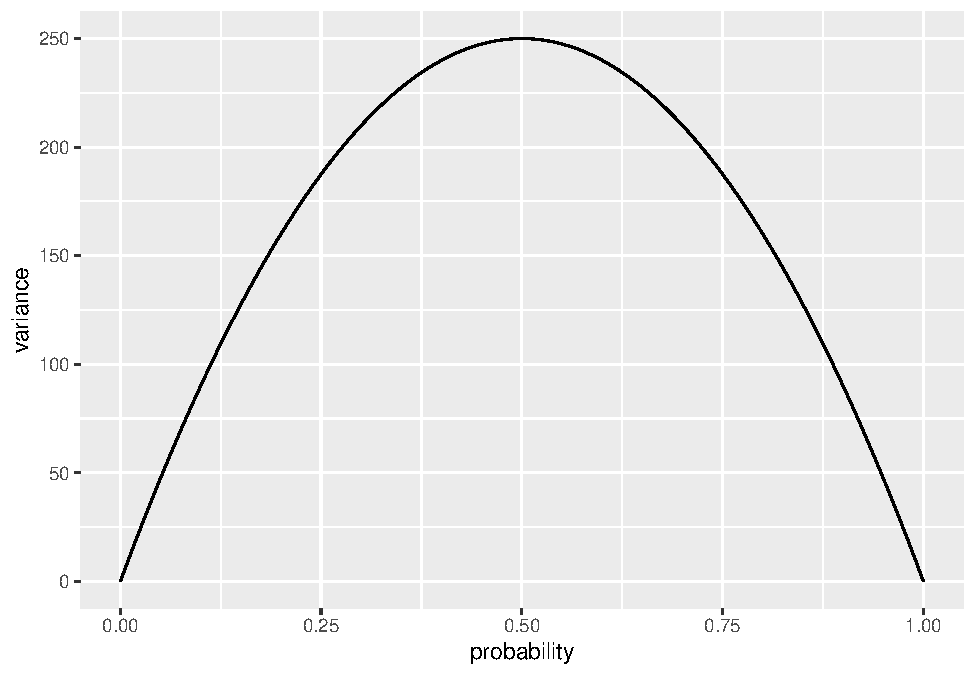
\includegraphics{08-广义线性混合效应模型_files/figure-latex/binomial-var-plot-1.pdf}
\caption{\label{fig:binomial-var-plot}方差与概率的关系图(\(n=1000\))}
\end{figure}

\hypertarget{ux5e7fux4e49ux7ebfux6027ux6a21ux578b}{%
\section{广义线性模型}\label{ux5e7fux4e49ux7ebfux6027ux6a21ux578b}}

广义线性模型{[}不要与一般线性模型(General Linear Models)混淆{]}的基本思想是指定一个\textbf{链接函数(link function)},将响应空间(response space)转换为建模空间(modeling space),这样我们可以执行常规线性回归,并通过\textbf{方差函数(variance function)}捕捉方差对均值的依赖性。模型的参数将在建模空间的尺度上表示,但我们总是可以使用\textbf{逆链接函数(inverse link function)}将其转换回原始的响应空间。

有很多不同类型的广义线性模型可以拟合不同类型的数据。在心理学中最常用的是\textbf{逻辑回归(logistic regression)}和\textbf{泊松回归(Poisson regression)},前者用于二分类数据(伯努利试验,Bernoulli trials),后者用于试验次数未明确规定计数数据。我们将重点关注逻辑回归。

\hypertarget{ux903bux8f91ux56deux5f52}{%
\section{逻辑回归}\label{ux903bux8f91ux56deux5f52}}

\hypertarget{ux672fux8bed}{%
\subsection{术语}\label{ux672fux8bed}}

\begin{tabular}{l|l}
\hline
Term & Definition\\
\hline
**伯努利试验** & 具有二元结果的事件,其中一个结果被认为是“成功”\\
\hline
**概率(proportion)** & 伯努利试验的成功次数与总次数之比\\
\hline
**发生比(odds)** & 成功对失败的比率\\
\hline
**对数发生比(log odds)** & 发生比的(自然)对数\\
\hline
\end{tabular}

注:odds也有人翻译为几率,考虑到几率表意并不直观,且易与概率(proportion)混淆,发生比又有些拗口,很多材料也不去翻译,所以本文之后直接使用odds和log odds。

在逻辑回归中,我们在log odds空间中建模响应变量与一组预测变量之间的关系。

逻辑回归用于个体结果是伯努利试验(具有二分类结果的事件)的情况。通常两种结果之一被称为``成功'',编码为1;另一种结果称为``失败'',编码为0。需要注意的是,``成功''和``失败''这两个术语是完全随意的,不应该认为更可取的类别总是编码为1。例如,当抛硬币时,我们可以同样选择``正面''为成功,``反面''为失败,反之亦然。

通常,伯努利试验序列的结果通过\textbf{概率}(成功次数与试验总次数的比率)来传达。例如,如果我们抛硬币100次,得到47次正面,那么我们的概率就是47/100或0.47,这也将是我们对事件可能性的估计。对于编码为1和0的事件,计算概率的便捷方法是使用\texttt{mean()}函数。

我们也可以谈论成功的odds,例如,正面与反面的odds是一比一,即1:1。格拉斯哥某天降雨的odds是170:195;分母是没有下雨的天数(365 - 170 = 195)。用小数表示,170/195约等于0.87,这被称为\textbf{natural odds}。natural odds的范围是0到\(+\infty\)。给定\(N\)次试验中成功\(Y\)次,我们可以将natural odds表示为\(\frac{Y}{N - Y}\)。或者,给定一个概率\(p\),我们可以将odds表示为\(\frac{p}{1-p}\)。

odds的自然对数,或\textbf{logit},是进行逻辑回归的尺度。回想一下,对某个值\(Y\)的对数给出在给定底数下使\(Y\)成立的指数。例如,16的\(log_2\)(以2为底的对数)是4,因为\(2^4 = 16\)。在逻辑回归中,通常使用的底数是\(e\)(也称为欧拉数,Euler's number)。例如,要从格拉斯哥降雨的odds中得到log odds,我们会使用\texttt{log(170/195)},其结果为-0.1372011;要从log odds中恢复natural odds,我们会使用逆运算\texttt{exp(-.137)},其结果约为0.872。

\hypertarget{log-oddsux7684ux6027ux8d28}{%
\subsection{log odds的性质}\label{log-oddsux7684ux6027ux8d28}}

log odds = \(\log \left(\frac{p}{1-p}\right)\)

log odds具有一些适用于线性建模的优秀性质。

首先,它是围绕0对称,且log odds等于0对应最大的不确定性,即概率为0.5。正的log odds意味着成功比失败更可能(成功的概率 \textgreater{} 0.5),负的log odds意味着失败比成功更可能(成功的概率 \textless{} 0.5)。log odds为2表示成功比失败可能性大的程度与-2表示失败比成功可能性大的程度相同。其尺度是无界的,范围从\(-\infty\)到\(+\infty\)。

\hypertarget{ux94feux63a5ux51fdux6570ux548cux65b9ux5deeux51fdux6570}{%
\subsection{链接函数和方差函数}\label{ux94feux63a5ux51fdux6570ux548cux65b9ux5deeux51fdux6570}}

逻辑回归的链接函数是:

\[\eta = \log \left(\frac{p}{1-p}\right)\]

而逆链接函数为:

\[p = \frac{1}{1 + e^{-\eta}}\]

其中\(e\)是欧拉数。在R中,In R, 你可以将逆链接函数写成:\texttt{1/(1\ +\ exp(-eta))}。

方差函数为二项分布的方差,即:

\[np(1 - p)\]

下面的app允许你在log odds空间中操控一条线的截距和斜率,并查看该线在响应空间中的投影。请注意该函数在响应空间中是S形(``sigmoidal'')。

\label{fig:logit-app}\textbf{逻辑回归网页app} \url{https://rstudio-connect.psy.gla.ac.uk/logit}

\hypertarget{ux5728rux4e2dux4f30ux8ba1ux903bux8f91ux56deux5f52ux6a21ux578b}{%
\subsection{在R中估计逻辑回归模型}\label{ux5728rux4e2dux4f30ux8ba1ux903bux8f91ux56deux5f52ux6a21ux578b}}

对于单层数据,可以使用\texttt{glm()}函数。请注意,这个函数与你已经熟悉的\texttt{lm()}函数非常相似。主要区别在于你需要为链接/方差函数指定一个\texttt{family}参数。对于逻辑回归,可以使用\texttt{family\ =\ binomial(link\ =\ "logit")}。二项分布的链接默认值是logit链接,因此只需输入\texttt{family\ =\ binomial}即可。

\texttt{glm(DV\ \textasciitilde{}\ IV1\ +\ IV2\ +\ ...,\ data,\ family\ =\ binomial)}

对于有随机效应的多层数据,可以使用\texttt{lme4}包中的\texttt{glmer}函数:

\texttt{glmer(DV\ \textasciitilde{}\ IV1\ +\ IV2\ +\ ...\ (1\ \textbar{}\ subject),\ data,\ family\ =\ binomial)}

  \bibliography{book.bib,packages.bib}

\end{document}
